\documentclass[11pt]{report}
\usepackage[utf8]{inputenc}
\usepackage[a4paper, total={6.5in, 9in}]{geometry}
\linespread{1.2}
\usepackage{amsmath}
\usepackage{amsthm}
%===== FONT ====%
\usepackage{palatino}
\usepackage{bm}
\usepackage{dsfont}
\usepackage{cancel}
\usepackage{amssymb}
\usepackage{commath}
\usepackage{mathtools}
\usepackage{float}
\usepackage{accents}
\usepackage{algorithm}


\usepackage[numbers]{natbib}
\bibliographystyle{abbrvnat}

\usepackage{subcaption}
\usepackage{graphicx}


\usepackage{color}
\usepackage{tcolorbox}
\usepackage{tikz}
\usetikzlibrary{matrix}
\newtcolorbox{mybox}[3][]
{
%   colframe = #2!25,
%   colback  = #2!10,
%   coltitle = #2!20!black,  
%   title    = {#3},
%   #1,
colframe = black,
  colback  = black,
  coltitle = white,  
  coltext = white,
  title    = {#3},
  #1,
}

\usepackage{xcolor}
\usepackage[colorlinks,linkcolor=blue,citecolor=blue,urlcolor = violet]{hyperref}

\usepackage[capitalise]{cleveref}%nameinlink,

% MATH OPERATOR
% Shortcuts
\def\be{\begin{equation}}
\def\ee{\end{equation}}

\def\bea{\begin{align}}
\def\eea{\end{align}}

\def\bea*{\begin{align*}}
\def\eea*{\end{align*}}
% Environments
% ------------
\theoremstyle{plain}
\newtheorem{theorem}{Theorem}[section]
\newtheorem{thm}[theorem]{Theorem}
\newtheorem{lemma}[theorem]{Lemma}
\newtheorem{corollary}[theorem]{Corollary}
\newtheorem{proposition}[theorem]{Proposition}
\newtheorem{asm}[theorem]{Assumption}
\theoremstyle{definition} % switch to 'definition' theorem style
\newtheorem{definition}[theorem]{Definition}
\newtheorem{example}{Example}%[theorem]
\newtheorem{remark}[theorem]{Remark}

\counterwithin{equation}{section}
\counterwithin{algorithm}{section}
\counterwithin{example}{section}

% Math Operator
\DeclareMathOperator{\A}{\mathbb{A}}
\DeclareMathOperator{\B}{\mathbb{B}}
\DeclareMathOperator{\C}{\mathbb{C}}
\DeclareMathOperator{\D}{\mathbb{D}}
\DeclareMathOperator{\E}{\mathbb{E}}
\DeclareMathOperator{\F}{\mathbb{F}}
\DeclareMathOperator{\G}{\mathbb{G}}
\DeclareMathOperator{\HH}{\mathbb{H}}
\DeclareMathOperator{\I}{\mathbb{I}}
\DeclareMathOperator{\J}{\mathbb{J}}
\DeclareMathOperator{\K}{\mathbb{K}}
\DeclareMathOperator{\LL}{\mathbb{L}}
\DeclareMathOperator{\M}{\mathbb{M}}
\DeclareMathOperator{\N}{\mathbb{N}}
\DeclareMathOperator{\OO}{\mathbb{O}}
\DeclareMathOperator{\Pb}{\mathbb{P}}
\DeclareMathOperator{\Q}{\mathbb{Q}}
\DeclareMathOperator{\R}{\mathbb{R}}
\DeclareMathOperator{\SSS}{\mathbb{S}}
\DeclareMathOperator{\T}{\mathbb{T}}
\DeclareMathOperator{\U}{\mathbb{U}}
\DeclareMathOperator{\V}{\mathbb{V}}
\DeclareMathOperator{\W}{\mathbb{W}}
\DeclareMathOperator{\X}{\mathbb{X}}
\DeclareMathOperator{\Y}{\mathbb{Y}}
\DeclareMathOperator{\Z}{\mathbb{Z}}
%======================================%
\DeclareMathOperator{\calA}{\mathcal{A}}
\DeclareMathOperator{\calB}{\mathcal{B}}
\DeclareMathOperator{\calC}{\mathcal{C}}
\DeclareMathOperator{\calD}{\mathcal{D}}
\DeclareMathOperator{\calE}{\mathcal{E}}
\DeclareMathOperator{\calF}{\mathcal{F}}
\DeclareMathOperator{\calG}{\mathcal{G}}
\DeclareMathOperator{\calH}{\mathcal{H}}
\DeclareMathOperator{\calI}{\mathcal{I}}
\DeclareMathOperator{\calJ}{\mathcal{J}}
\DeclareMathOperator{\calK}{\mathcal{K}}
\DeclareMathOperator{\calL}{\mathcal{L}}
\DeclareMathOperator{\calM}{\mathcal{M}}
\DeclareMathOperator{\calN}{\mathcal{N}}
\DeclareMathOperator{\calO}{\mathcal{O}}
\DeclareMathOperator{\calP}{\mathcal{P}}
\DeclareMathOperator{\calQ}{\mathcal{Q}}
\DeclareMathOperator{\calR}{\mathcal{R}}
\DeclareMathOperator{\calS}{\mathcal{S}}
\DeclareMathOperator{\calT}{\mathcal{T}}
\DeclareMathOperator{\calU}{\mathcal{U}}
\DeclareMathOperator{\calV}{\mathcal{V}}
\DeclareMathOperator{\calW}{\mathcal{W}}
\DeclareMathOperator{\calX}{\mathcal{X}}
\DeclareMathOperator{\calY}{\mathcal{Y}}
\DeclareMathOperator{\calZ}{\mathcal{Z}}
%======================================%
\DeclareMathOperator{\frakA}{\mathfrak{A}}
\DeclareMathOperator{\frakB}{\mathfrak{B}}
\DeclareMathOperator{\frakC}{\mathfrak{C}}
\DeclareMathOperator{\frakD}{\mathfrak{D}}
\DeclareMathOperator{\frakE}{\mathfrak{E}}
\DeclareMathOperator{\frakF}{\mathfrak{F}}
\DeclareMathOperator{\frakG}{\mathfrak{G}}
\DeclareMathOperator{\frakH}{\mathfrak{H}}
\DeclareMathOperator{\frakI}{\mathfrak{I}}
\DeclareMathOperator{\frakJ}{\mathfrak{J}}
\DeclareMathOperator{\frakK}{\mathfrak{K}}
\DeclareMathOperator{\frakL}{\mathfrak{L}}
\DeclareMathOperator{\frakM}{\mathfrak{M}}
\DeclareMathOperator{\frakN}{\mathfrak{N}}
\DeclareMathOperator{\frakO}{\mathfrak{O}}
\DeclareMathOperator{\frakP}{\mathfrak{P}}
\DeclareMathOperator{\frakQ}{\mathfrak{Q}}
\DeclareMathOperator{\frakR}{\mathfrak{R}}
\DeclareMathOperator{\frakS}{\mathfrak{S}}
\DeclareMathOperator{\frakT}{\mathfrak{T}}
\DeclareMathOperator{\frakU}{\mathfrak{U}}
\DeclareMathOperator{\frakV}{\mathfrak{V}}
\DeclareMathOperator{\frakW}{\mathfrak{W}}
\DeclareMathOperator{\frakX}{\mathfrak{X}}
\DeclareMathOperator{\frakY}{\mathfrak{Y}}
\DeclareMathOperator{\frakZ}{\mathfrak{Z}}



\newcommand{\rr}[1]{\textcolor{red}{#1}}
\newcommand{\bb}[1]{\textcolor{blue}{#1}}

% Keywords command
\providecommand{\keywords}[1]
{
  \small	
  \textbf{\textit{Keywords ---}} \textit{#1}
}

%========== Title ==========%
\usepackage{authblk}
\makeatletter
\renewcommand\AB@affilsepx{; \protect\Affilfont}
\makeatother
\renewcommand\Authfont{\large}
\renewcommand\Affilfont{\small}
\renewcommand\Authsep{, }


\usepackage[symbol]{footmisc}
\renewcommand{\thefootnote}{\fnsymbol{footnote}}

\usepackage{fancyhdr}
\pagestyle{fancy}

\fancyhf{}
\renewcommand{\headrulewidth}{0.2pt}

\fancyfoot[C]{\scriptsize\thepage}
\fancypagestyle{firststyle}
{
   \fancyhf{}
   \renewcommand{\headrulewidth}{0pt}
   \fancyfoot[C]{\scriptsize\thepage}
}

\date{\vspace{-1em}\normalsize{\today}}

\begin{document}
 
%=============================%
\begin{titlepage}

\phantom{h}
\vspace{1.5cm}

\centering{


\Large
Department of Operations Research and Financial Engineering\\
\vspace{0.6cm}
Princeton University \\ 
\vspace{1.2cm}
General Examination - Report\\
\vspace{1.2cm}
\huge
\textbf{Valuation of High-Dimensional and Path-Dependent Contingent Claims}\\

\vspace{1.2cm}
\LARGE
Valentin Tissot-Daguette\\
\Large
\vspace{1.2cm}
\Large
ORFE Adviser: Prof. H. Mete Soner
\\
Industry Mentor: Dr. Bruno Dupire
\\
\vspace{1cm}
\today\\
\vspace{3cm}

\includegraphics[scale=0.18]{Figures/Princeton Logo.png}
\hfill 

\includegraphics[scale=0.68]{Figures/small-orfe-logo.png}
}
\end{titlepage}
\renewcommand{\thefootnote}{\arabic{footnote}}
%=============================%
\cleardoublepage
\pagenumbering{roman}
\tableofcontents
%=============================%
%\listoffigures
%\listoftables
%=============================%
\cleardoublepage
\pagenumbering{arabic}
%\thispagestyle{firststyle}
\begin{center}
    \LARGE %\textbf{ High-dimensional American Options and Neural Parametrization of the Free Boundary}
    \textbf{Neural Parametrization of Free Boundaries in Optimal Stopping Problems}%Deep Stopping: The Free Boundary
    \\%\footnote[1]{Date: \today}} \\
    \vspace{0.5cm}
    \normalsize  A. Max Reppen\footnote[1]{Questrom School of Business, Boston University, Boston, MA, 02215, USA. } % Email: \texttt{\textbf{amreppen@bu.edu}}
    \quad H. Mete Soner\footnote[2]{Operations Research and Financial Engineering, Princeton University, Princeton, NJ 08540, USA.} % Department Email: \texttt{\textbf{soner@princeton.edu}}
    \quad  Valentin Tissot-Daguette\footnotemark[2]\\%{Operations Research and Financial Engineering   Department, Princeton University, Princeton, NJ 08540, USA. }\\ %Email: \texttt{\textbf{v.tissot-daguette@princeton.edu}}
\vspace{.2cm}
\today
\end{center}

\vspace{-2mm}
\begin{abstract}

\end{abstract}

\keywords{Free boundary problems, American derivatives, optimal stopping, deep learning }
\\

\textit{\textbf{MSC (2020) Classification —} 
\textnormal{91G20, %derivatives
91G60, %num. methods
68T07, %ANN
35R35. %Free Boundary Problem
}
}  

\renewcommand{\thefootnote}{\arabic{footnote}}
\chapter{Introduction}

Few words on option pricing (challenge etc)

Structure.




% \section{Framework and Notation}
% Let $\Lambda := \bigcup_{t\in[0,T]}\Lambda_t$,  with the Skorokhod spaces $\Lambda_t = \calD([0,t],\R^d)$ for some $T>0$ and $d\in \N$. Put another way, $\Lambda$ is the collection of all càdlàg paths  with various lengths.   In the financial applications, we will interpret $X$ as a vector of  stock prices or the random sources driving the latter.  Moreover, $T$ will usually seen as the maturity of a contingent claim.
% We adopt the following notation: Given $X_t\in \Lambda_t$, $X_s$ denotes the whole trajectory up to time $s\le t$, while $x_s= X_t(s)$ is the value at time $s$. We equip $\Lambda$ with a $\sigma-$algebra $\calF$, filtration $\F$ and probability measure $\Q$ %(e.g., the Wiener measure) 
% to form a stochastic basis $(\Lambda,\calF,\F, \Q)$. The price vector is therefore the coordinate process. 

%We therefore work with the canonical setting. 



\chapter{High-Dimensional Claims with Early Exercise}

%\section*{Introduction}
... 
Similar to \cite{Becker1,Becker2}, we solve the optimal stopping problem by employing the \textit{Deep Monte Carlo Optimization} method. This was  first introduced by \citet{HanJentzenE} to solve high-dimensional semilinear PDEs; see also \cite{Germain} for an error analysis and alternative schemes. The algorithm can be adapted to parametrize  stochastic controls \cite{HanE} (+Hure , Warin) yielding impressive results  in quadratic hedging  (Warin) and the  Merton portfolio problem  \cite{ReppenSoner}. See also \cite{ReppenSonerTissot} for a survey.     %, %together with continually improving computers, impressive approximation capabilities in recent years. 
 
 %showing impressive performance to approximate . \bb{...}
%========= Section 1 ==========%
\section{Optimal Stopping and Free Boundary Problems}


We fix throughout a time horizon $T>0$ and a probability space $(\Omega, \calF, \Q)$.  
Let us assume that the price vector $S = (S_t)_{t\in [0,T]}$, $S_t = (S_{t,1},...,S_{t,d}) \in \R_{+}^d$  is a c\`adl\`ag  process. 
We adopt the notation $\SSS_t = (S_u)_{u\in [0,t]}$ so that for 
$\Q-$almost every $\omega \in \Omega$,  $\SSS(\omega)$ belongs to $ \Lambda := \bigcup_{t\in [0,T]} \Lambda_t$ with the  Skorokhod spaces $\Lambda_t := \calD([0,t],\R^d_+).$ 

So far, it is not assumed that $S$ is a Markov process. Indeed, the dynamics of $S$ may depend on exogenous factors $\calV_t = (\calV_{t,1},...,\calV_{t,l}) \in \R^l$ (e.g. stochastic volatility, interest rate, volume, etc). However, we require that the enlargement $(S,\calV)$ is a c\`adl\`ag Markov  process with respect to its natural filtration, which we denote by $\F$. The probability space is henceforth filtered with $\F$. 

 
Moreover, let  $B=(B_t)_{t\in [0,T]}$ be the money market account and $D_{t,u} = \frac{B_t}{B_u}$ the 
discount factor over the interval $ [t,u]$. We  impose the mild restriction that $D_{t,u} \in [0,1]$ for all $0\le t \le u \le T$, i.e. $B$ is non-decreasing. This amounts to saying that interest rates are non-negative. 

\subsection{Optimal Stopping}
We  associate to any reward functional $\Phi: \Lambda \to \R$ and subset $\calT \subseteq [0,T]$ the \textit{optimal stopping problem}, 
\begin{equation}\label{eq:OS}
\underset{\tau \, \in \, \vartheta(\calT)}{\text{sup}} \ \E^{\Q}[D_{0,\tau}\, \Phi(\SSS_{\tau})],
\end{equation} 
where $\vartheta(\calT)$ is the set of $\F-$stopping times taking values in $\calT$. Notice that the factors $ (\calV_{\cdot,1},\ldots, \calV_{\cdot,l})$ (if any) do not appear in the payoff. We nevertheless observe $\calV$ (as $\F$ is the natural filtration of $\bar{S}$) which may influence our stopping decision. 

To make $\eqref{eq:OS}$ nontrivial,
it is often assumed that $\sup_{t \in \calT} \Phi(\SSS_{t}) \in L^1(\Q)$; see \cite{PeskirShiryaev}. Solving the optimal stopping problem without further assumptions on $\Phi$ proves hard as 
$(S,\Phi(\SSS),\calV)$ may fail to be a Markov process. 

To circumvent this issue, we impose the following condition on $\Phi$. 
\begin{asm}\label{asm:enlargement}
There exists $k\in \N$ and a vector-valued functional $\Upsilon: \Lambda \to \R^k$ such that
\begin{enumerate}
\item $Y := (\Upsilon(\SSS_t))_{t\in [0,T]}$ has c\`adl\`ag trajectories $\Q-$a.s. 
    \item $X := (S,Y,\calV)$ is a Markov process with state space $\calX \subseteq  \R^d_+ \times \R^{k} \times \R^{l}$.
    \item  $\Phi(\SSS_t) = \varphi(X_t)$ for some function $\varphi:\calX \to \R$ such that  $ \forall \ x=(s,y,\nu) \in \calX$,  $\varphi(x)$ does not depend on $\nu$.
\end{enumerate}
\end{asm}

When $\Phi$ is path-independent, the above assumptions are not needed and we simply set $k=0$ and $X=(S,\calV)$. With a slight abuse of notation, we may occasionally write $\varphi(x)=\varphi(z)$, where $x=(z,\nu)$ and  
\begin{equation} \label{eq:Z}
    z\in \calZ := \{(s,y) \in \R_+^d \times \R^k \ | \ (s,y,\nu) \in \calX \text{for some } \nu \in \R^k\}.
\end{equation} 
When $k=0$, we  may even use $\varphi(x)$ and $\varphi(s)$ interchangeably.  % and use $\Phi$ or $\varphi$ interchangeably. 
Problem $\eqref{eq:OS}$ can therefore be reformulated as follows:
\begin{equation}\label{eq:OS2}
\underset{\tau \, \in \, \vartheta(\calT)}{\text{sup}} \ \E^{\Q}[D_{0,\tau}\, \varphi(X_{\tau})].
\end{equation} 
Having now a Markovian framework, we can introduce the \textit{value function} associated to $\eqref{eq:OS2}$, that is
\begin{equation} \label{eq:valueFct}
v(t,x):= \underset{\tau \, \in\,  \vartheta(\calT_{\!t})}{\text{sup}} \
\E^{\Q}\! \left[ D_{t,\tau}\ \varphi(X^{t,x}_\tau)\ \right],\quad (t,x)\in [0,T]\times \calX,
\end{equation} %\underset{\tau \in \llbracket t,T \rrbracket}{\text{ess sup}}
with $\calT_{\!t} = \calT \cap \ [t,T]$ and $X^{t,x} = (X_u^{t,x})_{u\in [t,T]}$ denotes the forward-starting process such that $X^{t,x}_t= x \in \calX$.  We stress that  $\E^{\Q}\! \left[ D_{t,\tau}\ \varphi(X^{t,x}_\tau)\ \right]$ is understood as $\E^{\Q}\! \left[ D_{t,\tau}\ \varphi(X_\tau)\ | \ X_t= x\right]$.  %and the simplified notation $\E_{t,s}^{\Q}[\cdot]=\E^{\Q}[\cdot\,|\, S_t=s].$ 
The optimal stopping problem  $\eqref{eq:OS2}$ therefore consists of finding $v(0,\cdot)$.

When $\Q$ is a risk-neutral measure, $v$ is construed in finance as the price function of an \textit{option}  (or \textit{contingent claim}) with payoff $\varphi$ and exercise dates $\calT$. We will stick to this interpretation throughout this section and beyond.
Options are subdivided into roughly three families  characterized by their exercise style. More specifically, an option is called 
% \begin{itemize}
%     \item[(i)] \textit{European} if $\calT = \{T\}$,
%     \item[(ii)] \textit{Bermudan} if $\calT = \{t_1,\ldots,t_n\}$ where $0\le t_1 < \ldots < t_n \le T $, $n\in \N$,
%     \item[(iii)] \textit{American} if $\calT = [0,T]$.
% \end{itemize}
(i) \textit{European} if $\calT = \{T\}$, (ii) \textit{Bermudan} if $\calT = \{u_1,\ldots,u_n\}$, $0\le u_1 < \ldots < u_n \le T $, $n\in \N$, or (iii) \textit{American} if $\calT = [0,T]$. It is often assumed that any claim permits the holder to exercise at maturity, i.e. $T\in \calT$. In view of $\eqref{eq:valueFct}$, this ensures  that $v^{\text{European}} \le v^{\text{Bermudan}} \le v^{\text{American}} $, with the obvious notation.  Note that for European options, we simply have $v^{\text{European}}(t,x)= \E^{\Q}\! \left[ D_{t,T}\ \varphi(X^{t,x}_T)\ \right]$. We will therefore turn our attention to options of Bermudan or American type.

Although promising a continuum of exercise dates is idealistic, American options remain the most common product on derivatives markets and the most challenging from a mathematical standpoint. For options of American type, one is  forced to approximate the contract by a Bermudan option whose exercise dates cover $[0,T]$ (see \citet{Guyon}). The price is thereafter easily computed using Dynamic Programming. %Also observe that American contracts are idealistic as financial markets still operate in discrete time. However, American options present  great challenges and elegance from a mathematical standpoint.

%the function $\varphi$ is the \textit{payoff} of an option with early exercise and $v$ is its \textit{price}. 
It is clear that a rational agent would stop (or exercise) the contract at  $t\in \calT$ 
as soon as $v(t,x) \le \varphi(x)$. On such occasions, we in fact have $v(t,x) = \varphi(x)$ since $t$ is itself a stopping time and $\varphi(x) = \E^{\Q}\! \left[ D_{t,t}\ \varphi(X^{t,x}_t)\ \right] \le v(t,x)$. 
This brings us to the following definition. 
\begin{definition}
The \textit{stopping region} is defined as $\calS := \prod_{t\in \calT} \calS_t \subseteq \calT \times \calX$, with  the  $t-$sections 
\begin{equation}\label{eq:stopRegion}
    \calS_t:= \left\{ x \in \calX\ | \
v(t,x)=\varphi(x)\ \right\}, \quad t\in \calT\!.
\end{equation}
%When it is not optimal to stop, we are in 
Its complement 
is the 
the \textit{continuation region}, namely
$$\calC =\prod_{t\in \calT} \calC_t, \quad \calC_t:= \left\{ x \in \calX\ | \
v(t,x) > \varphi(x)\ \right\}. $$
\end{definition}

Notice in particular that $\calS_T=\R^d_+$ as the payoff and value function coincide at maturity.
\begin{remark}
The partition of $\calX$ into the stopping and continuation region is only made for dates at which the option can be exercised. Equivalently, one could have defined 
$\calS = \prod_{t\in [0,T]} \calS_t \subseteq [0,T]\times \calX$ ($\calC = \prod_{t\in [0,T]} \calC_t$) and set $\calS_t =\varnothing$ ($\calC_t =\calX$) whenever $t\notin \calT$. 
\end{remark}
As every Borel measurable subset $\calU \subseteq \calT \times \calX$ is paired with the hitting time $$\tau(\calU) := \inf\{t\in \calT \ | \ (t,X_t) \in \calU \}\wedge T,$$
it is easily seen that
\begin{equation}\label{eq:subset}
   v(0,X_0) =\underset{\calU \, \subseteq \, \calT \times \R^d_+}{\text{sup}} \, \E^{\Q}[D_{0,\tau(\calU)}\, \varphi(X_{\tau(\calU)})].  
\end{equation}
Indeed, $v(0,X_0)$ clearly dominates the right hand side of $\eqref{eq:subset}$, while  $\tau(\calS)= \inf\{t\in \calT \ | \ v(t,X_t)= \varphi(X_t) \} \wedge T$ is known to be the (smallest)   stopping time maximizing $\eqref{eq:OS}$; see, e.g., Theorem 2.2 in  \citet{PeskirShiryaev}. 

\subsection{Free Boundary}

The first connection between American options and free boundary problems is due to
\citet{mcKean}, a decade before the celebrated Black \& Scholes formula. We here state the result in a quite general framework. In what follows, we suppose that $X$ is in addition a Feller process. The infinitesimal generator of $S$ is denoted by $\calL: \calD_{\calL} \to \calC_0(\calX)$, where $\calD_{\calL}$ is its domain and $\calC_0(\calX) \subseteq \calC(\calX)$ the family of  continuous functions  vanishing at infinity.  
Moreover, we assume that the money market account is a deterministic process and write $$\hat{\varphi}(t,x):= D_{0,t}\ \varphi(x), \quad \hat{v}(t,x):= D_{0,t} \ v(t,x),$$
for the discounted reward and value function, respectively. As $D_{0,t}D_{t,u}=D_{0,u}$ for $0\le t \le u \le  T$, we simple have   $\hat{v}(t,x)= \sup_{\tau \, \in\,  \vartheta(\calT_{\!t})} \ \E^{\Q}\! \left[ \,  \hat{\varphi}(\tau, X^{t,x}_\tau)\ \right].$ We recall that the process 
$$\hat{v}(t,X_t)= \underset{\tau \, \in\,  \vartheta(\calT_{\!t})}{\text{ess sup}} \ \E^{\Q}\! \left[ \,  \hat{\varphi}(\tau, X^{t,x}_\tau)\ \right]\big |_{x=X_t}, \quad t \in [0,T],$$
is the \textit{Snell envelope} of $\hat{\varphi}(\cdot,X)$. % $ (\hat{\varphi}(t,X_t))_{t\in [0,T]}$. 
In other words, it is the smallest supermartingale dominating the discounted payoff process. We  now proceed to the main result of this section.  

\begin{theorem} Let $X$ be a Feller process with generator $\calL$. Then the discounted value function $\hat{v}$ associated to  $\eqref{eq:OS}$ solves the free boundary problem 
\begin{align}\label{eq:FB}
    \begin{cases}
    (\partial_t + \calL)\hat{v} \le 0 &  \text{on } [0,T] \times \calX,\\
    (\partial_t + \calL)\hat{v} = 0  & \text{on } \calC,\\
   \hat{v} \ge \hat{\varphi} & \text{on } [0,T] \times \calX,\\
    \hat{v}= \hat{\varphi}  & \text{on } \calS,
    \end{cases}
\end{align}
with  the terminal condition $\hat{v}(T,\cdot)= \hat{\varphi}$. Equivalently, $\eqref{eq:FB}$ can be expressed in variational form, namely 
$$ (\partial_t + \calL)\hat{v} \vee (\hat{\varphi} - \hat{v}) = 0.$$
\end{theorem}
Notice that a classical solution of the above free boundary problem  may not exist; see \citet{JLL} for a weak formulation \bb{(looking for an older reference in the PDE literature)}. 
The main difficulty of equation $\eqref{eq:FB}$ is that the stopping region $\calS$ (and in turn, $\calC$) is unknown and  part of the problem. 

In particular, the \textit{free boundary} $\partial \!  \calS$ is unknown. In this paper, 
 we propose to parametrize the latter. To be more accurate, we aim at finding the  reduced  boundary of each $t-$section $\calS_t$ in the interior of $\calX$, that is  
 $$\Gamma_t := \partial^*\! \calS_t \cap \, \mathring{\calX}.$$
 Focusing on the reduced boundary does not affect the value function and will simplify the parametrization. 
 \subsection{Motivation: A One-dimensional Example} \label{sec:1DExample}
 Let $d=1$ and consider an American call option, that is $\Phi(\SSS_t)=\varphi(S_t)=(S_t-K)^+$ where $K$ is the strike of the option. %\footnote{When no additional factor is needed, i.e. $X=S$, we rather use the letter $S$ to emphasize that it corresponds to the stock price.} 
 Furthermore, we choose the Black-Scholes model \cite{BS}, i.e. $S$ solves the SDE 
 $$\frac{dS_t}{S_t} = (r-\delta)dt + \sigma dW_t, \quad S_0\in \R_+,$$
 where $W$ is a $\Q-$Brownian motion and  $r\ge 0,\ \delta \ge 0 ,\ \sigma > 0$ represent the interest rate, dividend rate and volatility, respectively.  Clearly, no  state enlargement is needed so we can set $m=k=0$ and write $S$ instead of $X$.
We refer the interested reader to \citet{Karatzas} for a treatment of American contingent claims in the multi-asset Black-Scholes model. 
In a risk-neutral market, we must have $B_t=e^{rt}$, giving $D_{t,u} = e^{-r(u-t)}$. Moreover, the generator of $S$ reads $\calL = (r-\delta)s\,  \partial_s + \frac{1}{2}(\sigma s)^2\partial_{ss}$. 
The  stopping region is known to be of the form $$\calS = \prod_{t\in [0,T]} [f(t), \infty), $$
 %$\calS = \prod_{t\in [0,T]} [0,f(t)]$
 for some \textit{threshold function} $f:[0,T]\to [K,\infty)$  (see \cite{Merton,VB}).  The reduced boundary of $\calS_t$ is thus   the singleton $  \{f(t)\}$. %\Gamma_t =
 It is clear that $f$ is no less than the strike, as %otherwise the reward is nil and 
 $v$ is certainly positive prior to maturity.  %and holding the contract until maturity has positive value.  
% The smooth pasting condition $\eqref{eq:smoothPast}$ therefore reads
 %$$\partial_{s}v(t,f(t)) = \partial_{s}\varphi(f(t)) =  1, \quad t \in [0,T].$$
 
 Finding characteristics of the threshold function have been  the subject of many works. Among others, \citet{VB} showed the continuity of $f$ while \citet{Kim} proved that $f$ is non-increasing  with left limit %and satisfies 
 $f(T-) = K (1 \vee \frac{r}{\delta})$. %; to name a few. 
 If $r>0$,  the last property implies that $f(t) \uparrow \infty$ (hence $\calS_t \downarrow \varnothing$) as $\delta \downarrow 0$ for all $t<T$.  This is in line with the well-known fact that when interest rates are positive and the underlying doesn't issue dividends, the value of the American call coincide with its European counterpart; see \citet{Merton}. The exact expression  of $f$$-$if it exists$-$remains unknown to this day.
 %As negative interest rates were observed only recently, the bulk of the literature has focused on American put options. non dividend-paying
 %In addition, \citet{Barles} and \citet{Kuske} investigate the behaviour of the boundary near maturity. is in fact known \cite{Barles,Kuske} and given by $f(t) $

 In the same spirit of $\eqref{eq:subset}$, the initial price of the American call can be expressed as 
 \begin{equation*}
     v(0,S_0) = \underset{g\in \calG}{\text{sup}} \, \E^{\Q}[D_{0,\tau(g)}\, \varphi(S_{\tau(g)})],
 \end{equation*}
 where  $\calG = \calC([0,T], \R)$ and 
 $\tau(g) = \inf\{t\in [0,T] \ | \ S_t \ge g(t) \} \wedge T$. 
 Of course, maximizing over all functions in $\calG$ is computationally infeasible. Instead, we consider a family of (continuous) parametric functions $\calG_{p} = \{ G(\cdot, \theta) \ | \ \theta \in \Theta_p\} \subseteq \calG$ where $\Theta_p \subseteq \R^p$ is a compact parameter set. 
 Thus,   a lower bound of the initial price is given by
 \begin{equation}\label{eq:paramValue}
     v_0^p := \underset{\theta \in \Theta_p}{\text{max}} \calR(\theta)  ,
 \end{equation} 
 with the reward function
  \begin{equation}\label{eq:reward}
     \calR(\theta) =  \E^{\Q}[D_{0,\tau^{\theta}}\, \varphi(S_{\tau^{\theta}})], \quad   \tau^{\theta} = \tau(g^{\theta}).
 \end{equation} 
 Assuming that $\calG_p \to \calG$ when $p \to \infty$, we expect that $v_0^p \to v(0,\cdot)$ as well. %In this work, $\calG_p$ consists of \textit{feedforward neural networks}, presenting impressive approximation capabilities. 
 %This will be discussed in greater depth in \cref{sec:DMCO}.
   
 
 We close this section by illustrating the approach with a two-parameter family. Let
 %, and Bermudan put \cite{ Garcia}. % or of Bermudan type \cite{}.    %As the threshold function for \textit{perpetual} American options is known, it is
% For the American call, one can consider for instance the two-parameter family
 \begin{equation}\label{eq:twoParams}
     G(t,\theta) = K\left(1 \vee \frac{r}{\delta}+ \theta_1  \left(1-\frac{t}{T} \right)^{\theta_2} \right), \quad \theta = 
     (\theta_1,\theta_2) \in \Theta_2 = \R^2_+.
 \end{equation}
 %$$G(t,\theta) = K\left(1 \vee \frac{r}{\delta}\right)+ \theta_1  \left(1-\frac{t}{T} \right)^{\theta_2}, \quad (\theta_1,\theta_2) \in \Theta_2 = [0,1]\times \R_+.$$%=(\theta_1,\theta_2)^{\top}
 %\bb{Explanation + Figure showing different threshold functions (two-parameter family?) together with the optimal one. }
 Similar ansätze %involving few parameters %families with few parameters 
 have been 
 proposed %in the literature 
 for put options; see \cite{Garcia,Little}.  %\citet{Garcia} and  \citet{Little}. 
 Note that $G(\cdot,\theta)$ is non-decreasing with  $G(T-,\theta) = K(1 \vee \frac{r}{\delta})$ for all $\theta \in \Theta_2$. The initial level and curvature of the boundary is tuned with $\theta_1$ and $\theta_2$, respectively. % Barles, Kuske: focus on behaviour near maturity
 Figure \ref{fig:twoParams} shows the boundaries obtained from two parameter pairs for an out-of-the-money American call option ($s < K$) with $r\le \delta$. Notice how  lowering the boundary (right chart) significantly shifts the hitting times $\tau^{\theta}(\omega_1),\,\tau^{\theta}(\omega_2)$. % to the left. %The boundary in the right chart seem suboptimal as it forces the agent to exercise early.
 
 %The left chart seems more optimal than the right one.  although we won't pursue further numerical investigation at this stage.
 
 \begin{figure}
     \centering
     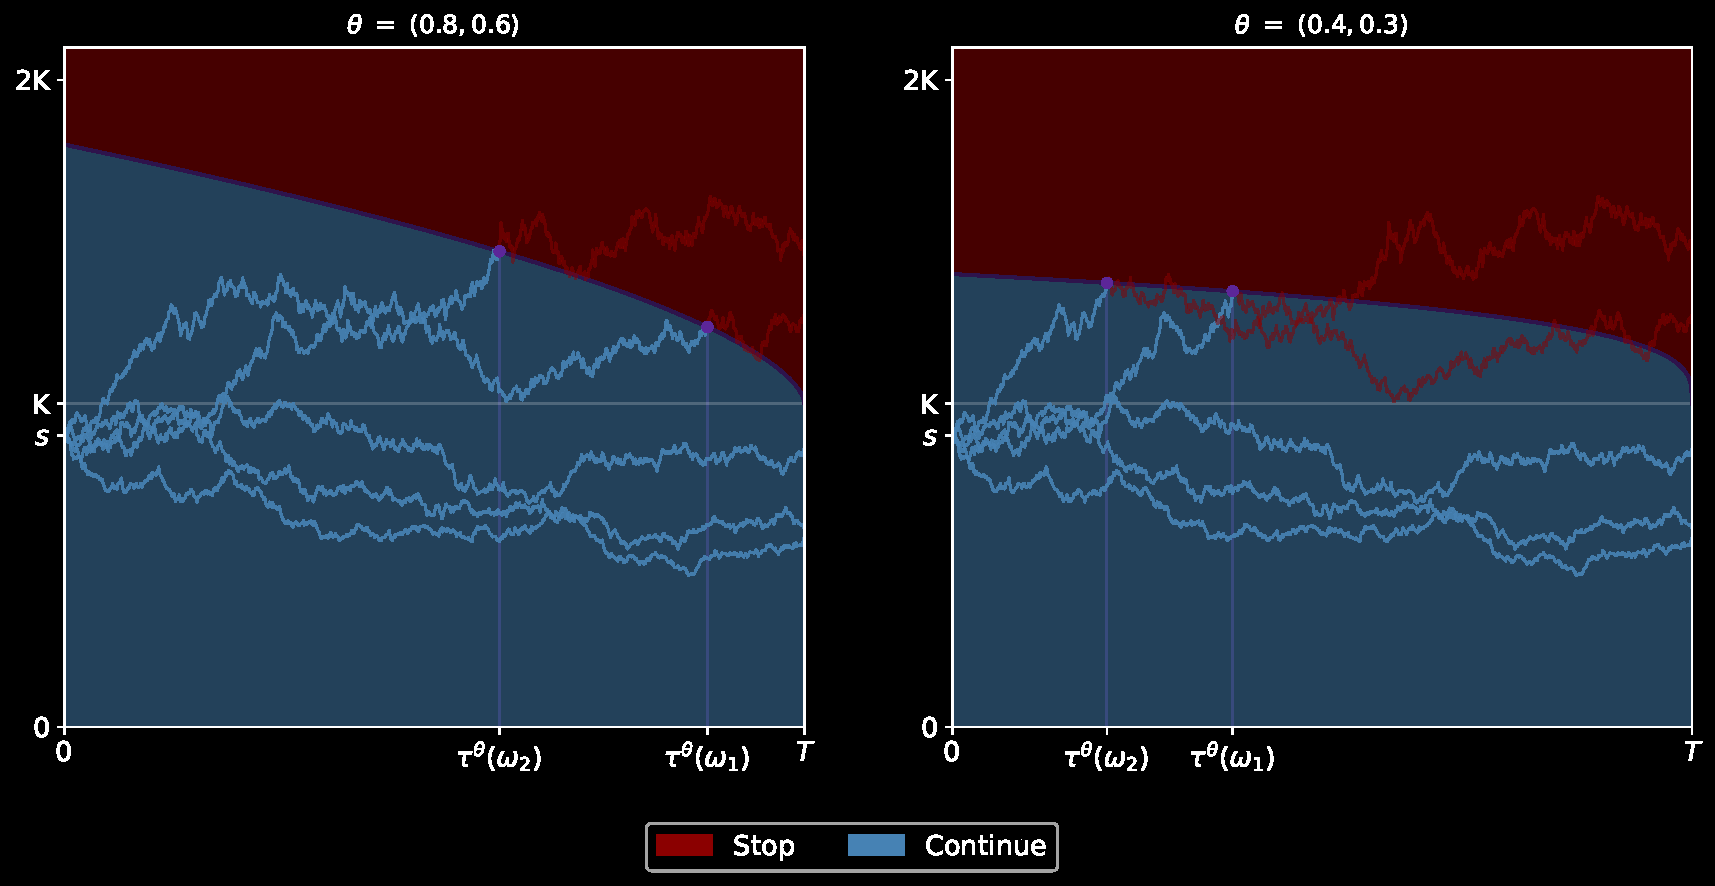
\includegraphics[scale=0.5]{FB/Figures/twoParams.pdf}
     \caption{Boundaries obtained from the two-parameter family $\eqref{eq:twoParams}$.}
     \label{fig:twoParams}
 \end{figure}
 
 

 
 
 
 %In the numerical examples, we will show how neural networks can be employed to parametrize the threshold function. 
 
 %\subsection{Motivation in the one-dimensional case}



%========= Section 2 ==========%
\section{Neural Parametrization}

\subsection{Representation of the Free Boundary}

In free boundary problems, %it is common to represent
the region sought can be represented locally, up to a rotation of axes, as the epigraph of a threshold function $f: [0,T]\times \calX \to \R$, namely
$$\calS_t = \{x\in \calX \,|\, x_{\bar{d}} \ge f(t,x_{-})\},$$
where $\bar{d}= \text{dim}(\calX)= d+m+k$,  $x_{-}=(x_1,...,x_{\bar{d}-1})$.
%See for instance \citet{Laurence}. 
The free boundary is thus formed by the points $x\in \calX$ satisfying  $x_{\bar{d}} = f(t,x_{-})$. We generalize this representation by considering other "separations" of $\calX$ as explained in the following assumption. %We make the following general assumption. 

\begin{asm}
\label{asm:star}
There exists a homeomorphism $A=(\alpha,\Xi) : \calX  \to \calA \times \calE$, $\calA = \alpha(\calX) \subseteq \R$, $\calE = \Xi(\calX)$  
% \begin{equation}\label{eq:homeo}
% A:=(\alpha,\Xi) : \calX  \to \calA \times \calE \subseteq \R \times \calX,  
% \end{equation}
%i.e. $\calA = \alpha(\calX), \ \calE = \Xi(\calX)$,  
satisfying the following property: If $x,x' \in \calX$ such that  $\Xi(x')=\Xi(x)$, then for $t\in [0,T]$,% and $s \in \calS_t$ for some $t \in [0,T]$, 
%we have 
\begin{equation*}
   x \in \calS_t \ \textnormal{ and } \ \ \alpha(x') \ge \alpha(x)  \; \Longrightarrow  \;
x' \in \calS_t.
\end{equation*}
\end{asm} 

In light of \cref{asm:star},  we define the \textit{threshold function} $
f: [0,T]\times \calE \to \R$  by 
% \begin{equation}\label{eq:threshold}
%   f(t,\xi) =
% \sup \calA_{t,\xi}, \quad  \calA_{t,\xi}=\{a \ge 0 \ | \ (a,\xi) \in \calZ \text{ and } A^{-1}(a,\xi)\in \calS_t\}. 
% \end{equation}

\begin{equation}\label{eq:thres}
   f(t,\xi) =
\inf \calA_{t,\xi}, \quad \calA_{t,\xi} = \{a \in \calA \ | \  A^{-1}(a,\xi)\in \calS_t\}. 
\end{equation}
The following result explains how the threshold function relates to the stopping region. 
%$The motivation of our approach is reinforced by the following lemma. 
\begin{proposition}\label{prop:thresStop}
Let $f$ as in $\eqref{eq:thres}$ and consider the subset $\frakS_t = \{x\in \calX \ | \ \alpha(x)  \ge f(t,\Xi(x)) \}.$
Then  for each $t\in [0,T]$, the following inclusions hold,
$$\mathring{\frakS}_t \subseteq \calS_t  \subseteq \frakS_t. $$ 
Moreover, if  $v$ is continuous, then $\calS_t = \frakS_t$ and 
$\partial \! \calS_t = \{x\in \calX \ | \ \alpha(x) = f(t,\Xi(x))\}$.
\end{proposition}
\begin{proof}
 First, assume that $x \notin \calS_t$. Then $\alpha(x) \notin \calA_{t,\xi}$ with $\xi := \Xi(x)$. Since $a\in \calA_{t,\xi}$ implies  $a'\in \calA_{t,\xi}$ for all $a' \ge a$, we conclude that  $\alpha(x) \le  \inf \calA_{t,\xi} = f(t,\xi)$ and
 $\mathring{\frakS}_t \subseteq \calS_t$ follows. For the second inclusion, suppose that $x\in \calS_t$. Then $\alpha(x) \in \calA_{t,\Xi(x)}$,  which immediately gives $\alpha(x) \ge f(t,\Xi(x))$. Thus $\calS_t \subseteq \frakS_t$ as well. Finally, when $v$ is continuous, then $\calS_t$ is a closed subset of $\frakS_t$ that contains $\mathring{\frakS}_t$, hence $\calS_t = \frakS_t$.
\end{proof}

We recall that under mild assumptions on $X$,  %(namely that  $X$ is stationary), 
the stopping region expands over time, i.e. $\calS_t \subseteq \calS_{t'}$ whenever $t\le t'$; see \cref{prop:monot}. 
It follows from \cref{prop:thresStop}  that   $t\mapsto f(t,\xi)$ must be non-increasing for all $\xi\in \calE$.  %; see \cref{prop:monot} and \cref{cor:monot}. 

To solve the optimal stopping problem, the above construction suggests to parametrize the threshold function, namely 
\begin{equation}
    f(t,\xi) \approx G(t,\xi; \theta), \quad G(\cdot,\cdot; \theta) \in \calG_p, 
\end{equation}
with $\calG_p = \{G(\cdot,\cdot; \theta) \ | \ \theta \in \Theta_p \}$ and compact parameter subset $\Theta_p \subseteq \R^p$, $p\in \N$. This gives, in turn, the parametrized free boundary 
$\Gamma_t^{\theta} = \{x \in \mathring{\calX} \ | \ \alpha(x) = G(t,\Xi(x); \theta)\}. $ 
The stopping time associated to $\theta \in \Theta_d$ is therefore
\begin{equation}\label{eq:stopTime}
    \tau^{\theta} = \inf\{t \in [0,T] \ | \ \alpha(X_t) \ge G(t,\Xi(X_t); \theta) \} \wedge T,
\end{equation}
with associated reward  $\calR(\theta)$ as defined  in $\eqref{eq:reward}$.

% \begin{example}\label{ex:1DExample2}
% Consider the standard American call option example discussed in \cref{sec:1DExample}. Then \cref{asm:star} is fulfilled with the homeomorphism $A = (\alpha,\Xi)$ given by $\alpha(s) = s$ and $\Xi \equiv 0$. Indeed, we have seen in \cref{sec:1DExample} that $\calS_t$ is a right-unbounded interval, hence $s\in \calS_t$ and  $s' = \alpha(s') \ge \alpha(s) =s$ implies that $s'\in \calS_t$ as well.  As $\Xi$ is constant, the threshold function $G(\cdot;\theta)$ depends solely on time for fixed $\theta$. Therefore, the stopping time in $\eqref{eq:stopTime}$ simply reads $$\tau^{\theta} = \inf\{t \in [0,T] \ | \ S_t \ge G(t; \theta) \} \wedge T.$$
% %$$v(t,s') $$  %$\calS = \prod_{t\in [0,T]} [f(t), \infty), $ for some threshold function $f:[0,T]\to [K,\infty)$.  

% %Indeed, if $s\in \calS_t$ and $s' = \alpha(s') \ge \alpha(s) =s$, then 
% %$$v(t,s') $$

% \end{example}

\subsection{Deep Monte Carlo Optimization} \label{sec:DMCO}
We adapt the \textit{Deep Monte Carlo Optimization} algorithm \cite{HanJentzenE} to our framework. Let $\calG_p$ be a family of feedforward neural networks  with a total of $p$ parameters. If the optimal threshold function $f$ is continuous, then the universal approximation property of neural networks  \cite{Cybenko,Hornik} guarantees the existence of $p\in \N$ and parameter $\theta \in \Theta_p$ such that $G(\cdot,\cdot;\theta)$ is arbitrarily close to $f$.  %In particular, if $v_0^p$ is the value function as in $\eqref{eq:paramValue}$, we expect that  $v_0^p \to v(0,\cdot)$ as $p \to \infty$. 

To find a near-optimal parameter vector, we employ  \textit{stochastic gradient ascent} (SGA), which we explain now. First, we discretize time along a partition $\Pi_N = \{0 = t_0 < \ldots < t_N=T\}$, $N\in \N$. Therefore, the stopping times $\tau^{\theta}$ in $\eqref{eq:stopTime}$ take value in   $\calT_N = \calT \cap \ \Pi_N$. %\calT_N := 
If there are finitely many exercise date, we simply set $\Pi_N = \calT$, i.e. $\calT_N = \calT$. 
Second, the reward function $\calR$ in $\eqref{eq:reward}$ is replaced by its empirical counterpart, namely
\begin{equation}\label{eq:empReward1}
    \hat{\calR}_B(\theta) = \frac{1}{B}\sum_{j=1}^B   D_{0,\tau^{\theta,j}}  \ \varphi(X_{\tau^{\theta,j}}^j),
\end{equation}
where $B\in \N$ is the \textit{batch size} and  $\tau^{\theta,j}$ denotes the realized  stopping time as in $\eqref{eq:stopTime}$ for the $j-$th trajectory. Next, 
starting with initial weights  $\theta^{(0)}\in \Theta_p$ (e.g. generated randomly), we iteratively update the parameter vector  according to 
\begin{equation}\label{eq:SGA}
\theta^{(m)} = \theta^{(m-1)} + \zeta_m \nabla \hat{\calR}(\theta^{(m-1)}), \quad m=1,\ldots, M,  
\end{equation}
with \textit{learning rates} $(\zeta_m)$. 
%The number of training iterations $M\in \N$ is either fixed or 
However, applying the stochastic gradient method as in $\eqref{eq:SGA}$ will not work because the stopping time relies on a binary decision.  Indeed, assuming that the distribution of $X_t$ is atomless and $\alpha$ is nowhere constant, then an infinitesimal shift of the boundary will not alter the sign of  $\alpha(X^{j}_{t_n}) - G(t_n,\Xi(X^{j}_{t_n}); \theta)$. In turn, the corresponding stopping time and  reward will remain unchanged. 
Hence, $\nabla \hat{\calR}$ vanishes and the SGA method fails to  converge to a (local) maximum. 
The remedy is to relax the stopping decision, as  explained in the next section. % by considering \textit{fuzzy boundaries}

\subsection{Fuzzy Boundary and Relaxed Stopping}

\begin{algorithm}[t]
\label{alg:FBTrain}
\caption{Free Boundary Training}\label{alg:cap} 
\begin{enumerate}
\setlength \itemsep{0.05ex}
\vspace{-3mm}

\item \textbf{Initialize} $\theta^{0} \in \Theta_p$
%\textbf{Given} $\theta^{(0)} \in \Theta$, $\epsilon >0$, $M \in \N$
\item \textbf{For} $m = 0,\ldots, M-1$
    \begin{itemize}
    \setlength \itemsep{0.4ex}
    \vspace{-2mm}
        \item \textbf{Simulate} trajectories $(X_{t_n}^j)_{n=0}^N$, $\ j=1,\ldots,B$.
        \item %\textbf{For} $j = 1,\ldots, B$  
        \textbf{Compute} the
        \vspace{-3mm}
\begin{align*}
-&\text{ signed distances:} \quad &\delta^{\theta^{m}, j}_n &=  G(t_n,\Xi(X^j_{t_n}),\theta^{m}) \ - \ \alpha(X^j_{t_n}) \\[1em]
-&\text{ stopping factors:}\quad &p^{\theta^{m},\epsilon,j}_{n} &= h(\delta^{\theta^{m}, j}_n/\epsilon) \\[1em]
 -&\text{ stopping probabilities:}\quad &P^{\theta^{m},\epsilon,j}_{n} &= p^{\theta^{m},\epsilon,j}_{n}(1-q^{\theta^{m},\epsilon,j}_{n}) \quad  \text{($q^{\theta^{m},\epsilon,j}_{n}$ as in $\eqref{eq:recStop}$)}\\[0.2em]
    -&\text{ reward function:}\quad &\hat{\calR}_B^{\epsilon}(\theta^{m}) &=  \frac{1}{B}\sum_{j=1}^B  \sum_{n=0}^N D_{0,t_n}   P^{\theta^{m},\epsilon,j}_{n}\ \varphi(X_{t_n}^j)
    \end{align*}
%       \begin{itemize}
%       \setlength \itemsep{2ex}
% \item Signed distances: $\delta^{\theta^{m}, j}_n =  G(t_n,\Xi(X^j_{t_n}),\theta^{m}) \ - \ \alpha(X^j_{t_n}) $

% \item Stopping factors: $p^{\theta^{m},\epsilon}_{n} = h(\delta^{\theta^{m}, j}_n/\epsilon) $

%         \item Stopping probabilities: $P^{\theta^{m},\epsilon,j}_{n} = p^{\theta^{m},\epsilon,j}_{n}(1-q^{\theta^{m},\epsilon,j}_{n}) $, with $q^{\theta^{m},\epsilon,j}_{n}$ as in $\eqref{eq:recStop}$
%         \item Reward function: $\hat{\calR}_B^{\epsilon}(\theta^{m}) =  \frac{1}{B}\sum\limits_{j=1}^B  \sum\limits_{n=0}^N D_{0,t_n}   P^{\theta^{m},\epsilon,j}_{n}\ \varphi(X_{t_n}^j)$
%     \end{itemize}
          \vspace{-4mm}
          
        \item \textbf{Update:} $\theta^{m+1} = \theta^{m} + \zeta_m \nabla \hat{\calR}_B^{\epsilon}(\theta^{m})$
    \end{itemize}
\item \textbf{Return} $\theta^{M}$
\vspace{-3mm}

\end{enumerate}
\end{algorithm}

Instead of a sharp interface, we introduce a region,  called the \textit{fuzzy boundary}, where the binary decision ($1:$  stop, $0:$ continue) is replaced by a value in $(0,1)$. %agent chooses to stop with a certain probability. 
To this end,  we compute the signed distances to the boundary, namely
 \begin{equation}
     \delta^{\theta}_n =  G(t_n,\Xi(X_{t_n}),\theta) \ - \ \alpha(X_{t_n}), \quad n=0,\ldots ,N-1. 
 \end{equation}
 These are converted into \textit{stopping factors}  
$p^{\theta,\epsilon}_n := h(\delta^{\theta}_n /\epsilon), $ $\epsilon \ge 0$, where $h:\R \to [0,1]$ is a continuous function such that $h \equiv 1$ on $(-\infty,-1]$,  $h \equiv 0$ on $[1,\infty)$ and decreasing in $(-1,1)$. One can take for instance $h(\delta) = \frac{(1-\delta)^+ }{2} \wedge 1$. This gives the following  relaxed stopping decision for each $n\in\{0,\ldots,N-1\}$, 
$$ \begin{cases}
p^{\theta,\epsilon}_n = 1, & \text{ if } \  \delta^j_n \le -\epsilon,  \quad \text{(stopping region)}\\%ping region
p^{\theta,\epsilon}_n \in (0,1), & \text{ if } \   |\delta_n^{j}| < \epsilon, \hspace{0.4 mm} \quad \text{(fuzzy boundary)}\\
p^{\theta,\epsilon}_n = 0, & \text{ if } \  \delta^j_n \ge \epsilon. 
\hspace{3.5 mm} \quad \text{(continuation region)}%ation region
\end{cases} $$
At maturity, i.e.  $n=N$, we can simply set $p^{\theta,\epsilon}_N \equiv 1$. % as the option has to be exercised. 
The hyperparameter $\epsilon$ thus determines the "width" of the fuzzy boundary. %Moreover, the sharp interface is recovered by letting $\epsilon \downarrow 0$. 

Thereafter, let $q^{\theta,\epsilon}_{n} \in [0,1]$ be the probability that the option has been exercised before time $t_n$, i.e. $\tau^{\theta} < t_n$. Then the values of $q^{\theta,\epsilon}_{n}$  are obtained thanks to the recursive formula, 
\begin{align}\label{eq:recStop}
     q^{\theta,\epsilon}_{0} = 0, \quad 
     q^{\theta,\epsilon}_{n+1}
     = \underbrace{q^{\theta,\epsilon}_{n}}_{ \tau^{\theta} < t_n} + \underbrace{p^{\theta,\epsilon}_{n}(1-q^{\theta,\epsilon}_{n})}_{\tau^{\theta} = t_n}, \quad n = 0, \ldots, N-1. 
\end{align}
Clearly, $n \mapsto q^{\theta,\epsilon}_{n}$ is non-decreasing and equal to $1$ if $X$ strictly enters the stopping region, i.e.  $\delta^j_n \le -\epsilon$.   
The probability of stopping at time $t_n \in \calT_{\!N}$  is thus $P^{\theta,\epsilon}_{n} := p^{\theta,\epsilon}_{n}(1-q^{\theta,\epsilon}_{n})$. Finally,  the  reward obtained with the  fuzzy boundary is given by 
% \begin{enumerate}
% \item $h$ is continuous and non-decreasing,
%     \item $h(\delta) = 0 $ for $\delta \le -1$,
%     \item $h(\delta) = 1 $ for $\delta \ge 1$.
% \end{enumerate}

\begin{equation}\label{eq:empReward2}
\hat{\calR}_B^{\epsilon}(\theta) =  \frac{1}{B}\sum_{j=1}^B  \sum_{n=0}^N D_{0,t_n}   P^{\theta,\epsilon,j}_{n}\ \varphi(X_{t_n}^j),
\end{equation}
and $\eqref{eq:empReward1}$ is recovered by letting $\epsilon  \downarrow 0$. 
The training phase is summarized in \cref{alg:cap}. To compute the initial value of the optimal stopping problem, we choose a large number of simulations $J\in \N$ and use the sharp boundary formulation $\eqref{eq:empReward1}$, i.e.   
$ \hat{v}_0 = \hat{\calR}_J(\theta^{(M)}) .$ 
%If one is interest in the whole  value function, %—that is, the price of the American option over time—
 %we simply set $\hat{v}(t,s) := \E^{\Q}[D_{t,\tau^{\theta^*}}\, \varphi(S^{t,s}_{\tau^{\theta^*}})]$ where $\theta^*$ is the "trained" parameter from $\eqref{eq:paramValue}$. 
 \begin{remark}
 Note that the value function is also  available at any intermediate time $t\in \calT_{\!N}$ once the threshold function has been trained. Indeed, one  can set 
 $\hat{v}(t,s) = \frac{1}{J}\sum_{j=1}^J   D_{t,\tau_t^{\theta,j}}  \ \varphi(X_{\tau_t^{\theta,j}}^j),$ 
 with $$\tau_t^{\theta,j} = \inf\{u \in \calT_{N} \cap \, [t,T]\ | \ \alpha(X_u) \ge G(u,\Xi(X_u); \theta) \} \wedge T.$$
 \end{remark}
 
%  \begin{equation}\label{eq:stopTime}
%     \tau_t^{\theta,j} = \inf\{u \in \calT_t \ | \ \alpha(X_u) \ge G(u,\Xi(X_u); \theta) \} \wedge T.
% \end{equation}


%   \begin{remark}
%  If one is interest in the whole  value function, %—that is, the price of the American option over time—
%  we can simply set $v^p(t,s) := \E^{\Q}[D_{t,\tau^{\theta^*}}\, \varphi(S^{t,s}_{\tau^{\theta^*}})]$ where $\theta^*$ is the "trained" parameter from $\eqref{eq:paramValue}$. 
%  \end{remark}
 
\subsection{Importance Sampling}
%As the training of the treshold function is made by exploring the reward obtained when hitting the boundary 

%As the training phase relies on the reward obtained when hitting the boundary, it is crucial that the simulated paths explore the state space frequently enough. 

%\label{eq:empReward2}

% Note that 

% As the training phase relies on the reward obtained when stopping, 

%Otherwise, the threshold function may not be trained properly. 
To properly train the threshold function in \cref{alg:cap}, 
%In light of \cref{alg:cap},
it is  crucial  that the simulated paths $\alpha(X^{j})$ hit the (fuzzy) boundary frequently enough and  across exercise dates. 
% Indeed, the reward 
% As the empirical reward $\eqref{eq:empReward2}$ , Moreover,  and across the exercise dates. Otherwise, 
This can be achieved using importance sampling, as explained below.  %technique, as explained below. %by changing the drift of the stock prices adequately, as explained below. 

Let $W$ be a $d-$dimensional Brownian motion under $\Q$ and suppose that $S$ evolves according to the stochastic differential equation, 
% \begin{align*}
%     dS_t = \mu(t,S_t) dt + \sigma(t,S_t) dW_t, \quad S_0 \in \R,
% \end{align*}
\begin{align}\label{eq:stockSDE}
    dS_t = \mu_t dt + \sigma_t dW_t, \quad S_0 \in \R,
\end{align}
where $\mu$ (resp. $\sigma$) is a  $d-$dimensional  (resp. $\R^{d\times d}-$valued) process that may depend on $t,S_t$ and other exogenous factors. 
Then consider the Girsanov transformation 
\begin{equation}\label{eq:Girsanov}
\frac{d\Q^{\lambda}}{d\Q} = \calE_T(- \lambda \bullet W), \quad \lambda  \text{ predictable},\quad   \E^{\Q}\left[\exp\left(\frac{1}{2}\lVert \lambda\rVert^2_{L^2([0,T];\R^d)}\right)\right] <\infty, 
\end{equation}%\E^{\Q}\left[e^{\frac{1}{2}\int_0^T \lVert \lambda_t\rVert^2 dt}\right] <\infty,  $$
so that 
$W_t^{\lambda} :=  \int_0^{t}\lambda_s ds + W_t$ is Brownian motion under $\Q^{\lambda}$. Therefore, $S$ has $\Q^{\lambda}-$dynamics
\begin{equation}
    dS_t = \mu^{\lambda}_t dt + \sigma_t dW^{\lambda}_t,\quad \mu^{\lambda}_t = \mu_t - \sigma_t \lambda_t. 
\end{equation}
If we define $Z^{\lambda}_t = \frac{d\Q}{d\Q^{\lambda}} \big |_{\calF_t}  = \calE_t(\lambda \bullet W^{\lambda})$, then the expected reward associated to some $\tau \in \vartheta(\calT)$ reads  $\E^{\Q}[D_{0,\tau}\, \varphi(X_{\tau})] =  \E^{\Q^{\lambda}}[Z^{\lambda}_{\tau}D_{0,\tau}\, \varphi(X_{\tau})]. $ %In turn, 
% \begin{equation*}\label{eq:OS}
%  \E^{\Q}[D_{0,\tau}\, \varphi(X_{\tau})] =  \E^{\Q^{\lambda}}[Z^{\lambda}_{\tau}D_{0,\tau}\, \varphi(X_{\tau})]. 
% \end{equation*}
%This produces only a minor change in 
In turn, 
the empirical reward $\eqref{eq:empReward2}$ becomes 
\begin{equation}\label{eq:empReward3}
\hat{\calR}_B^{\epsilon,\lambda}(\theta) =  \frac{1}{B}\sum_{j=1}^B  \sum_{n=0}^N Z^{\lambda,j}_{t_n} D_{0,t_n}   P^{\theta,\epsilon,j}_{n}\ \varphi(X_{t_n}^j).
\end{equation}
The process $\lambda$ can be chosen so as to increase the probability of crossing the boundary before maturity. In the numerical experiments, the process $\lambda$ is assumed to be constant for simplicity; see for instance  \cref{sec:putBS,sec:maxCallSym}. Therefore, $\lambda$ is in this case seen as a hyperparameter vector. %at some specific date %$t\in \calT$ 
%or 
%within a given time interval. We illustrate the use of importance sampling with a one-dimensional example.   %Also, we may wish to ensure that the 
%in some time interval $B \in \calB([0,T])$, i.e. $\Q^{\lambda}(\tau \in B)$ % or simply before maturity. 

% \begin{example}  Let $d=1$ and consider a standard call option  in the Black-Scholes model as in \cref{sec:1DExample}, i.e.  $\varphi(s)=(s-K)^{+}$ and choose  $\mu_t = (r-\delta)S_t$,  $\sigma_t = \sigma S_t$ in $\eqref{eq:stockSDE}$ . We recall from  \cref{ex:1DExample2} that  
% the threshold function does not depend on $S$ and the associated stopping time is   $\tau^{\theta} = \inf\{t\in [0,T] \ | \ S_t \ge G(t;\theta)\}$.

% We here show how importance sampling permits to control the probability of hitting the boundary strictly before maturity. That is, for a target probability $q\in [0,1]$, we would like to find $\lambda \in \R$ such that 
% \begin{equation}\label{eq:target}
% \Q^{\lambda}(\tau^{\theta} \leq T) = q, 
% \end{equation}
% with $\Q^{\lambda}$ given in $\eqref{eq:Girsanov}$. Of course, this cannot be guaranteed for all parameter vector $\theta$ simultaneously, so we instead require that $\eqref{eq:target}$ holds approximately. To this end, we employ an initial guess from the two parameter family given in $\eqref{eq:twoParams}$. Assuming that $\delta \ge r$, then we choose 
%  \begin{equation*}
%      f_0(t) = K\left(1  + \theta_1  \left(\frac{t}{T} \right)^{\theta_2} \right), \quad \theta = 
%      (\theta_1,\theta_2) \in \Theta_2 = \R^2_+.
%  \end{equation*}
 
 
% $X^{\lambda}_t = e^{Y^\lambda_t}$, with the log price given by $$Y^{\lambda}_t = \log x_0 +  (r-\sigma^2/2 - \lambda\sigma ) t  + \sigma W^\lambda_t. \qquad (W^\lambda: \, \Q^\lambda-\text{Brownian motion})$$


% Assume the initial exercise boundary to be of the form 
% $$f(t) = f_0^{\,1-t/T}\,K^{t/T} \; \Longrightarrow \; \log f(t) = \log f_0 + \frac{t}{T} \log \frac{K}{f_0}, $$
% so that $f(0)=f_0<x_0$ and $f(T)=K$. If $q \in [0,1]$ denotes the target probability of crossing the boundary before $T$, find $\lambda = \lambda(x_0)$ s.t.
% $\Q^{\lambda}(\tau \leq T) = q,$
% with $$ \tau = \inf\{t\in [0,T] \,|\, X_t^\lambda \leq f(t)\}. \quad (\inf\,  \emptyset = \infty)$$ Observe that 
% $$
% X_t^\lambda \leq  f(t) \; \Longleftrightarrow \;  Y_t^\lambda \leq \log f(t)
% \; \Longleftrightarrow \;  W^\lambda_t + \tilde{\xi} t \leq \tilde{\alpha},
% $$
% where \vspace{-3mm}
% \begin{align*}
%     \tilde{\xi}&=\xi/\sigma, \quad \xi = r-\sigma^2/2 - \lambda \sigma - \frac{1}{ T} \log \frac{K}{f_0},\\\vspace{-3mm}
%     \tilde{\alpha}&=\alpha/\sigma, \quad \alpha =  \log \frac{f_0}{x_0} <0.
% \end{align*}
%  Girsanov implies that $W^ {\tilde{\xi}} := (W^\lambda_t +  \tilde{\xi} t)_{t\in [0,T]}$ is a standard BM under
% $$\Q^{\tilde{\xi}} (d\omega) = \mathring{Z}_T \Q^\lambda(d\omega), \quad  \mathring{Z}_{\cdot} = \calE_{\cdot}(-\tilde{\xi} \bullet W^\lambda).$$
% Therefore, using the distribution of passage times for BMs with drift (\citealp{KaratzasShreve}, section 3.5 C),
% \begin{align*}
%     \Q^{\lambda}(\tau \leq T) &= \E^{\Q^{\tilde{\xi}} }[\mathring{Z}^{-1}_T\, \mathds{1}_{\{\tau \leq T\}}]
%     = \E^{\Q^{\tilde{\xi}} }[\mathring{Z}^{-1}_{\tau }\, \mathds{1}_{\{\tau \leq T\}}]
%     = \int_0^T \frac{|\alpha|}{\sqrt{2 \pi t^3\sigma^2}}\exp\left\{- \frac{(\alpha - \xi t)^2}{2 t \sigma^2}\right\} dt.
% \end{align*}
% %We can solve numerically for $\lambda$ (located in $\xi$)  by setting the above expression equal to our target $q$. Figure \ref{fig:Girsanov} displays the function $x_0 \mapsto \lambda(x_0)\cdot \sigma$ for $q \in \{0.75,0.90\}$.
% \end{example}



%\subsubsection{Regularity}
%\citet{Laurence}, \citet{Costantini}


%\subsection{Convergence}
%========= Section 3 ==========%
\section{Applications in Finance}

%\subsection{Level Set Representation}
Let us present how our method applies to common contracts traded on options exchanges or over-the-counter. % (OTC). 
Throughout this section,  the payoff function is assumed to be  of the form%\footnote{With a slight abuse of notation, we may also write $\varphi(z), \ \alpha(z), \, \beta(z)$ with $x=(z,\nu)$.   } 
\begin{equation}\label{eq:payoff}
    \varphi(x) = \left( \eta  (\alpha(x) - \beta(x)-K)\right)^+, \quad x = (z,\nu), 
\end{equation}
where $\alpha, \beta: \calX \to \R_+$ 
are nonnegative projection maps independent of $\nu$. Recall that we may regard $\varphi$ as a function of $z$ only and the same holds for $\alpha$ and $\beta$.  %Again, we assume that 
The function $\beta$ is used to encompass spread options (\cref{ex:spread}) and  floating strike options (\cref{ex:Asian,ex:lookback}). Moreover, the parameter  $\eta \in \{\pm 1\}$ determines the option type (call  if $\eta=1$ and  put  if $\eta=-1$).
%This class of payoffs encompasses vanilla and most of the exotic options. 

%\subsection{Complete Markets}
%options and the most common exotic derivatives.  %\bb{(We may impose this structure later but this covers already many payoffs, including exotic ones as shown in the examples below)} 
  With little assumptions on $\alpha,\beta$, we can derive a useful geometric property of the stopping region, termed \textit{ray-connectedness} by  \citet{BroadieDetemple}. %
We first need a scaling property on the  process  $Z_t = (S_t,Y_t) \in \calZ$, $t\in[0,T]$,  with $\calZ$ defined in $\eqref{eq:Z}$. 

% \begin{asm} \label{asm:scale}
%     Given $0\le t \le u \le T$, the stochastic flow $z \mapsto Z_u^{t,z}$  scales  linearly, i.e. %in the sense that 
%     $Z_u^{t,\gamma z} = \gamma Z_u^{t,z}$ $\ \forall \ \gamma \ge 0$.
% \end{asm}

\begin{asm} \label{asm:scale}
    Given $0\le t \le u \le T$ and $\calV_t = \nu$, the stochastic flow $z \mapsto Z_u^{t,(z,\nu)}$  scales  linearly, i.e. 
    $Z_u^{t,(\gamma z,\nu)} = \gamma Z_u^{t,(z,\nu)}$ $\ \forall \ \gamma \ge 0$.
\end{asm}

% \begin{asm} \label{asm:scale}
%     Given $0\le t \le u \le T$ and $\nu \in \calV$, the stochastic flow $z \mapsto X_u^{t,(z,\nu)}$  scales  linearly, i.e. 
%     $X_u^{t,(\gamma z,\nu)} = \gamma X_u^{t,(z,\nu)}$ $\ \forall \ \gamma \ge 0$.
% \end{asm}

The next result is an adaptation of  Proposition A.5 in  \cite{BroadieDetemple}. 

\begin{proposition}
\label{prop:star}
Let $\eta =1$ and assume that $\alpha,\beta$ are homogeneous in $z$, i.e. $\pi(\gamma z)=\gamma \pi(z)$  for all $\gamma>0$,  $\pi \in \{\alpha,\beta\}$. Then \cref{asm:star} holds with the homeomorphism
%If  $\alpha$ is also continuous and positive on $\calX \setminus \{\boldsymbol{0}\}$, 
%then the map 
\begin{equation}\label{eq:homeo}
A=(\alpha,\Xi): \calX  \mapsto \calA \times \calE, \quad 
\Xi(x) = \left(\frac{z}{\alpha(z)},\nu\right), \quad x = (z,\nu). 
\end{equation}
%where $\calA \subseteq \R_+$ and $\calE \subseteq $
% : \calX  \mapsto \calA \times \calE
%with $x = (z,\nu)$, $z = (s,\nu)$. 
%defines a homeomorphism 
%with the following property: If $x,x' \in \calX$ such that  $\Xi(x')=\Xi(x)$, then for $t\in [0,T]$,% and $s \in \calS_t$ for some $t \in [0,T]$, 
%we have 
% \begin{equation*}
%   x \in \calS_t \ \textnormal{ and } \ \ \eta(\alpha(x') - \alpha(x)) \ge 0  \; \Longrightarrow  \;
% x' \in \calS_t.
% \end{equation*} 
 Put differently,  $(z,\nu)\in \calS_t$ implies that $(\gamma z,\nu) \in \calS_t$ for all $\gamma > 1$.
%$$x\in \calS_t \Longrightarrow \gamma x \in \calS_t$$ for any $\gamma > 1$
% \begin{enumerate}
%     \item For a call payoff ($\eta =1$) then $x\in \calS_t \Longrightarrow \gamma x \in \calS_t$ for any $\gamma > 1$.
%     \item For a put payoff ($\eta =-1$) then $x\in \calS_t \Longrightarrow \gamma x \in \calS_t$ for any $\gamma \in (0,1)$.
% \end{enumerate}
\end{proposition} 
\begin{proof}
First, the map $A$ given in $\eqref{eq:homeo}$ is clearly a homeomorphism. Indeed, its inverse $A^{-1}(a,\xi) = (a \xi_z,\xi_\nu)$, $\xi = (\xi_z,\xi_\nu) \in \calE$ is well-defined and continuous. Now let  $x = (z,\nu)$, $x' =(z',\nu')$  such that $\Xi(x')=\Xi(x)$ and $\alpha(z') \le \alpha(z)$. Consequently,   $z'= \gamma z$ with $\gamma := \frac{\alpha(z')}{\alpha(z)} \ge 1$ and $\nu = \nu'$. 

Next, assume that $x\in \calS_t$ for some $t\in [0,T]$. For any  stopping time $\tau \in \calT_{\!t}$, observe for $\pi \in \{\alpha,\beta\}$ that 
$$\pi(X^{t,x'}_{\tau})=\pi(Z^{t,(z',\nu)}_{\tau})=\pi(\gamma Z^{t,(z,\nu)}_{\tau})=\gamma \pi(X^{t,x}_{\tau}), $$ 
using Assumption \ref{asm:scale} and the homogeneity of $\pi$.
Therefore, we obtain
\begin{align*}
    \E^{\Q}\left[ D_{0,\tau} \varphi(X^{t,x'}_{\tau})\right] &= \E^{\Q}\left[ D_{0,\tau} \left(\alpha(X^{t,x'}_{\tau}) -\beta(X^{t,x'}_{\tau}) -K\right)^+ \right]\\
    &= \E^{\Q}\left[ D_{0,\tau} \left(\gamma \alpha(X^{t,x}_{\tau}) -\gamma \beta(X^{t,x}_{\tau}) -K\right)^+ \right]\\
   &\le \gamma \E^{\Q}\left[ D_{0,\tau} \varphi(X^{t,x}_{\tau}) \right] + (\gamma  - 1)K\\
   &\le \gamma \ \varphi(x) + (\gamma  - 1)K\\
   &= \varphi(x').
\end{align*}
In the first inequality, we used  $D_{t,u} \le 1$ and the subadditivity of $x \to x^+$. In the last equality, we noticed that the positive part  in $\varphi$ can be dropped as $x$ belongs to the  stopping region. %Hence $x'\in \calS_t$ and 
%The proof is complete.

\end{proof}

\begin{remark}
For put payoffs, i.e. $\eta =-1$,  \cref{prop:star} applies with the same homeomorphism but different conclusion, namely  $(z,\nu)\in \calS_t \Longrightarrow (\gamma z,\nu) \in \calS_t$ for all $\gamma \in (0,1)$. Moreover, the threshold function $\eqref{eq:thres}$ is given instead by 
$f(t,\xi) = \sup \calA_{t,\xi}$ and is  non-decreasing in $t$  thanks to the time  monotonicity of $\calS$ with respect to  $\subseteq$ (\cref{prop:monot}). 
\end{remark}


\begin{remark}
We recall that the optimal stopping decision is also achieved by comparing %the \textit{intrinsic value}, namely
$\varphi(x)$, oftentimes called the \textit{intrinsic value}, to the \textit{continuation value}
\begin{equation} \label{eq:contValue}
c(t,x) := \underset{\tau \, \in\,  \vartheta(\calT_{t+})}{\text{sup}} \
\E^{\Q}\! \left[ D_{t,\tau}\ \varphi(X^{t,x}_\tau)\ \right],\quad  \calT_{t+} = \calT_t \setminus\{t\}, \quad (t,x)\in [0,T]\times \calX.
\end{equation}
Using $\eqref{eq:payoff}$ and the fact that $\varphi(x)>0$ when $x\in \calS_t$, $t<T$, we obtain for call options that  
$$x \in \calS_t \ \Longleftrightarrow \ \varphi(x) \ge c(t,x) \ \Longleftrightarrow \ \alpha(x) \ge K + \beta(x) + c(t,x).$$
Thus, $f(t,\Xi(x)) = K+ \beta(x)  +  c(t,x)$. The knowledge of the threshold function is therefore equivalent to the knowledge of the continuation value.  Parametrizing  the latter
 has given rise to efficient pricing algorithms as demonstrated by \citet{LSMC} using least square regression and 
 \citet{Kohler} using neural networks.
%Among other methods, the continuation value is at the core of the \citet{LSMC} algorithm, where it is estimated using least square regression. %how our approach differs. 
The key advantage of our  approach  is the guarantee of producing  rational decisions$-$in the sense of Proposition \ref{prop:star}$-$as we exploit the geometric structure of the problem. %thanks the exploitation of the geometric structure of the problem which   %for any given parameter vector $\theta$.  
\end{remark}

%This rather obscure condition will be illustrated with several examples.
%We now 
%discuss several examples. 
%\subsection{Examples}\label{sec:examples}

\subsubsection*{Path-independent Payoffs}
Let us now present important families of path-independent payoffs. Unless stated otherwise,  we assume that no exogenous factors are needed  and write $X=S$. %and Assumption \ref{}. 

\begin{example}\label{ex:vanilla}

Consider vanilla  options of American type.  %example discussed in \cref{sec:1DExample} in an arbitrary model.
Then \cref{asm:star} is fulfilled with the homeomorphism $A = (\alpha,\Xi)$ given by $\alpha(s) = s$, $\beta \equiv 0$ and $\Xi(s) \equiv 1$. %Indeed, we have seen in \cref{sec:1DExample} that $\calS_t$ is a right-unbounded interval, hence $s\in \calS_t$ and  $s' = \alpha(s') \ge \alpha(s) =s$ implies that $s'\in \calS_t$ as well. 
As $\Xi$ is constant, the threshold function $f$ depends solely on time, as we shall see in  \cref{sec:putHeston}.   In a factor model, i.e. $x = (s,\nu)$, we have instead $\alpha(x)=s$, and $\Xi(x) \equiv (1,\nu)$. For a put option, this implies that $(s,\nu) \in \calS_t$ if and only if $s\le f(t,\nu)$; see \cref{sec:putHeston}.   

% and the stopping time in $\eqref{eq:stopTime}$ simply reads  $\tau^{\theta} = \inf\{t \in [0,T] \ | \ S_t \ge G(t; \theta) \} \wedge T.$ 
%As $\Xi$ is constant, the threshold function $G(\cdot;\theta)$ depends solely on time for fixed $\theta$. Therefore, the stopping time in $\eqref{eq:stopTime}$ simply reads $$\tau^{\theta} = \inf\{t \in [0,T] \ | \ S_t \ge G(t; \theta) \} \wedge T.$$
\end{example}

%For the following high-dimensional examples, we assume for simplicity that no exogenous factors are needed (i.e. $l=0$) and write $X=S$. 
%For simplicity, we assume that no exogenous factors are needed (i.e. $l=0$) and write $X=S$. %and Assumption \ref{}. 

\begin{example}\label{ex:bskt}
Consider the class of \textit{basket} options,
$$
\varphi(s)= \left( \eta \left( w^{\top} s - K \right) \right)^{+},
$$
with  weight vector $w$  belonging to the simplex $\Delta_{d} := \{w \in [0,1]^d \ | \ w^\top \mathds{1}=1\} $.
A generalization is given by \textit{index options} where the weights are allowed to vary over time. An example would be a vanilla option written on the S\&P $500$. % where the loadings are proportional to the market capitalization of the underlying stocks. 
In light of $\eqref{eq:payoff}$, we thus choose $\alpha(s) =  w^{\top} s$ and $\beta \equiv 0$. %Furthermore, as $w^\top \Xi(s) = \frac{w^\top s}{\alpha(s)}=1$ for all $s\in \R_+^d$,  
Notice that the image of  $\Xi$ is given by 
$\calE = \{ \xi \in \R_+^d \ | \ w^{\top} \xi =1 \}.$ 
When the weights are uniform, i.e. $\alpha(s) = \frac{1}{d}\sum_{i=1}^d s_i$, the payoff is symmetric in the underlying assets and satisfy interesting properties as outlined in . 

\end{example}

\begin{example}\label{ex:max}
\textit{Max-options} are call options  on the best-performing stock, that is
$$
\varphi(s)= \left(  \max_{i=1,...,d} s_i - K  \right)^{+}.
$$
This gives $\alpha(s)=\max_{i=1,...,d} s_i$ and $\beta\equiv 0$.  
%The subspace $\calE = \{\frac{s}{\alpha(s)} \ | \ s\in \R_+^d\}$ consists of the faces of the $d-$dimensional hypercube not containing the origin. %with at least one coordinate equal to $1$. 
%Hence, 
Moreover, observe that 
$\calE$  is formed by the faces of the  hypercube $[0,1]^d $ not containing the origin. %= \{\xi \in  [0,1]^d \ | \ \max_{i=1,...,d}\xi_i =1 \}

This seemingly innocent family of payoffs reveals many counterintuitive results, as beautifully articulated by \citet{BroadieDetemple}. Among other things, the authors showed that it is never optimal to prematurely exercise a max-call option when more than one asset attains the maximum. In the case $d=2$, this means that the diagonal $\{s \in \R^2_+ \ | \  s_1 = s_2\}$ is entirely contained in the continuation region prior to maturity. As we shall see in \cref{sec:maxCallSym},  the stopping region consists of one connected
component on each side of the diagonal. 

%As the payoff is symmetric, we therefore expect that $\calS_t$, if non-empty,  must be  disconnected for all $t<T$. 
Max-options have become a standard for numerical methods of high-dimensional options; see \cite{Becker1,Becker2} and references therein. 
%We will investigate this contract in further depth in the subsequent sections. 
In contrasts, \textit{put} options on the maximum of $d$ assets are less popular in the literature due to their low premium and are not discussed here. 
Also, one can imagine an option on the \textit{minimum} of several underlyings; see \cite[Chapter 6]{DetempleBook} and \cite{DetempleMin} for a thorough treatment in the two-dimensional case. %of min-call options on two assets.
% illustrate this fact and investigate other propthe 
\end{example}

\begin{example}\label{ex:spread}
Consider the family of \textit{spread options} \cite{Carmona},  that is 
$$
\varphi(s)= \left( \eta  \left ( s_1 - \sum_{i=2}^{d}\gamma_i s_i - K \right) \right)^{+},
$$
where  $(\gamma_{i})_{i=2}^d \in \R^{d-1}_+$ are conversion factors. We naturally set $\alpha(s)=s_1$, $\beta(s)=\sum_{i=2}^{d}\gamma_i s_i$. The corresponding homeomorphism is therefore given by 
$A=(\alpha,\Xi)$ with  $\Xi(s)=\frac{s}{s_1}.$ The threshold function thus depends on all stock prices expressed in terms of $s_1$. 
Choosing an asset as numéraire %(here $s_1$)  
was originated by \citet{Margrabe} for exchange options (i.e. the case $d=2$  and $\gamma_2=1$). 
\end{example}

% Let us verify
% that Assumption \ref{asm: homeomorph} holds with $\alpha$ defined above. As in the proof of Proposition \ref{prop:star}, take $s\in \calS_t$ for some $t\in [0,T]$ and $s'\in \R^d_+$ such that  $\frac{s}{s_1}=\frac{s'}{s'_1}$ and $s_1' \ge s_1$. For any stopping time $\tau \in \calT_{t}$, we obtain similarly
% \begin{align*}
%     \E^{\Q}\left[ D_{0,\tau} \varphi(S^{t,s'}_{\tau})\right] &= \E^{\Q}\left[ D_{0,\tau} \left(\psi_1\,  S^{t,s'}_{\tau,1} - \sum_{i=2}^{d}\psi_i S^{t,s'}_{\tau,i} -K\right)^+ \right]\\
%      &= s'_1\E^{\Q}\left[ D_{0,\tau} \left(\psi_1\,  S^{t,\Xi(s')}_{\tau,1} - \sum_{i=2}^{d}\psi_i S^{t,\Xi(s')}_{\tau,i} -\frac{K}{s_1'}\right)^+ \right]\\
%     &\le \E^{\Q}\left[ D_{0,\tau} \left(\gamma \pi(X^{t,x}_{\tau}) -K\right)^+ \right]\\
%   &\le \gamma \E^{\Q}\left[ D_{0,\tau} \left( \pi(X^{t,x}_{\tau}) -K\right)^+ \right] + (\gamma  - 1)K\\
%   &\le \gamma \left( \pi(x) -K\right) + (\gamma  - 1)K\\
%   &= \varphi(x').
% \end{align*}

% \begin{align*}
%     \E_t\left[ \varphi(t,S_{\tau}^{t,s})\right] &= s_1 \E_t\left[e^{-r\tau} \left(\frac{K}{s_1}+   \frac{\psi_2}{d-1}\sum_{i=2}^{d} S^{i,t,\Xi(s)}_{\tau} - \psi_1 S^{1,t,\Xi(s)}_{\tau} \right)^+ \right]\\
%     &\leq  s_1 \E_t\left[e^{-r\tau} \left(\frac{K}{s'_1}+   \frac{\psi_2}{d-1}\sum_{i=2}^{d} S^{i,t,\Xi(s')}_{\tau} - \psi_1 S^{1,t,\Xi(s')}_{\tau} \right)^+ \right] + K e^{-rt}\left(1- \frac{s_1}{s_1'}\right)^+\\
%     &=  \frac{s_1}{s_1'} \E_t\left[e^{-r\tau} \left(K+   \frac{\psi_2}{d-1}\sum_{i=2}^{d} S^{i,t,s'}_{\tau} - \psi_1 S^{1,t,s'}_{\tau} \right)^+ \right]+ K e^{-rt}\left(1- \frac{s_1}{s_1'}\right) \quad (s_1\leq s_1' )\\
%     &\leq \frac{s_1}{s_1'} \varphi(t,s')+ K e^{-rt} \left(1- \frac{s_1}{s_1'}\right)\\
%     &= e^{-rt}\left(K + \frac{\psi_2}{d-1}\sum_{i=2}^{d} \frac{s'_{i}}{s_1'}s_1 - \psi_1 s_1 \right)\\
%     &= e^{-rt}\left(K + \frac{\psi_2}{d-1}\sum_{i=2}^{d} s_{i} - \psi_1 s_1 \right) \quad (\text{since } \Xi(s)=\Xi(s'))\\
%     &= \varphi(t,s),
% \end{align*}
% %This is inspired from the Margrabe's technique for exchange options \cite{Margrabe} to set a stock as numéraire. % and express all assets  in terms of the latter. 
 

% \end{example}

%\subsubsection*{Path-dependent Payoffs}

\subsubsection*{Path-dependent Claims}

%We finish this 
%section with path-dependent claims. 
We assume throughout that $d=1$, although multi-asset path-dependent options may exist (see  Example \ref{ex:Asian}). % (e.g. an American Asian call on an equity index). 
%We now have to specify path-dependent variable

\begin{example}\label{ex:Asian}
\textit{Asian options} %(see \citet{Hull}, Section 25.12) 
are %vanilla 
derivatives with payoff involving the running average of the  underlying asset(s).  With this in mind, it is therefore natural to set $Y_t=\Upsilon(\SSS_t) = \frac{1}{t} \int_0^t S_u du$. It is easily seen that $X=(S,Y)$ is a Markov process.
There are two types of Asian payoffs, namely (i) Fixed strike: $\varphi(x) = \left(\eta (y - K)\right)^{+}$ and (ii) Floating strike:  $\varphi(x) = \left(\eta (s - \gamma y)\right)^{+}$ ($\gamma$: scaling factor).
% \begin{enumerate}
%     \item Fixed strike: $\varphi(x) = \left(\eta (y - K)\right)^{+}$.
%     \item Floating strike:  $\varphi(x) = \left(\eta (s - \gamma y)\right)^{+}$, where $\gamma$ is a scaling factor.
% \end{enumerate}

The projection functions are therefore $\alpha(x)=y$, $\beta \equiv 0$ and  $\alpha(x)=s$, $\beta(x) = \gamma y$ for fixed and floating strike options, respectively. %Although not covered in the numerical experiments, 
A multi-dimensional extension  could be obtained for instance by replacing the underlying by a stock index, e.g.
$$ \Phi(\SSS_t) = \left( \frac{1}{t} \int_0^t w_u^{\top} S_u du - K\right)^{+}, \quad S_u\in \R^d, \quad w_u\in \Delta_{d},\quad d\ge 2.$$

%Proposition \ref{prop:star} clearly applies, giving the homeomorphism
%$A=(\alpha,\Xi)$, with $\alpha = \pi$ and $\Xi(x) = (\frac{s}{y},1)$. 
%The threshold function will therefore depend on the ratio $\frac{S_t}{Y_t}$, which is used characterized the trend of the stock in path-dependent volatility models (cite Guyon)

%The first coordinate of the process $\Xi(X_t)=\frac{x}{y}$ is the ratio $\frac{S_t}{Y_t}$, 
% which is used characterized the trend of the stock in path-dependent volatility models (cite Guyon)?
\end{example}


\begin{example}\label{ex:lookback}
\textit{Lookback options} %(see \citet{Hull}, Section 25.10) %allows its holder to get
provides exposure to the minimum or maximum values attained by the stock so far. This suggests to choose $$Y_t=\Upsilon(\SSS_t) = \left(\max_{u\in[0,t]} S_u,\min_{u\in[0,t]} S_u\right).$$
It is easily seen that $X=(S,Y)$ is a  Markov process with state space $\calX = \{x=(s,y_1,y_2) \in \R_+^3 \ | \ y_2 \le s \le y_1\}$. Both fixed and floating contracts exist as in Example \ref{ex:Asian}. The most common contracts with their corresponding projection functions are listed in Table \ref{tab:lkbk}. The scaling factor $\gamma$ appearing in the payoff of floating strike options is introduced to reduce the price of these otherwise expensive contracts. We therefore choose $\gamma \in [1,\infty)$ and $\gamma \in (0,1]$ for call and put options, respectively.  
When $\gamma=1$, the payoff of a floating strike lookback call (put) option is precisely the %time $t$ 
drawdown (drawup) of the stock. See \citet{DaiKwok} for a thorough treatment of American lookback claims.  

%Note that the stopping decision relies on the size of the relative drawdown or drawup. 

\begin{table}[H]
    \centering
    \begin{tabular}{r|c|c|c}
        Option & $\Phi(\SSS_t)$ & $\alpha(x)$ & $\beta(x)$ \\ \hline \hline
         Fixed Strike Call & $(\max_{u\in[0,t]} S_u - K)^{+} $ & $y_1$ & $0$ \\[0.2em] \hline
       Fixed Strike Put & $(K - \min_{u\in[0,t]}S_u )^{+} $ & $y_2$ & $0$ \\[0.2em] \hline
        Floating Strike Call & $S_t - \gamma\min_{u\in[0,t]} S_u$  & $s$ & $\gamma  y_2$ \\[0.2em] \hline
        Floating Strike Put & $\gamma\max_{u\in[0,t]} S_u - S_t$ & $\gamma y_1$ & $s$ \\[0.2em] \hline \hline
    \end{tabular}
    \caption{Lookback Options, $x=(s,y_1,y_2)$.}
    \label{tab:lkbk}
\end{table}

%In addition, the projection functions are the same.
\end{example}


% \begin{remark}
% Floating strike options. The general form is
% $$
% \Phi(\SSS_t):= \left( \eta  \left [ S_t - k\Psi(\SSS_t) \ \right] \right)^{+},
% $$
% where $\Psi$ is typically the running maximum (floating lookback) or the average (floating Asian) and $k$ is a scaling factor. 
% We therefore set $Y_t=\Upsilon(\SSS_t) = \Psi(\SSS_t)$, $\alpha(x) = s$ and $\beta(y)=ky$. 

% \end{remark}

% \begin{example}
% \bb{\textit{Barrier options}}. Given in Table \ref{tab:barrier}. We can  set  $Y_t=\Upsilon(\SSS_t) = (\max_{u\in[0,t]} S_u,\min_{u\in[0,t]} S_u)$, $\beta \equiv 0$ and $\alpha$ as in the right column of Table \ref{tab:barrier}. As $\alpha$ is not homogeneous (and often $0$ for calls) we cannot apply Proposition \ref{prop:star}. Moreover, the stopping region is ray-connected for some payoffs (e.g. Up & and In Call) but not all (e.g. Up \& Out Call). \bb{Is it worth mentioning this class? }
% \end{example}

% \begin{table}[H]
%     \centering
%     \begin{tabular}{r|c|c}
%         Option & $\Phi(\SSS_t)$ & $\alpha(s,y_1,y_2)$  \\ \hline \hline
%          Up \& In Call & $(S_t - K)^{+} \mathds{1}_{\left\{\max_{u\in[0,t]} S_u \ge B\right\}}$ & $s \mathds{1}_{\{y_1 \ge B\}}$ \\ \hline
%         Up \& Out Call & $(S_t - K)^{+} \mathds{1}_{\left\{\max_{u\in[0,t]} S_u \le B\right\}}$ & $s \mathds{1}_{\{y_1 \le B\}}$ \\ \hline
%       Down \& In Call & $(S_t - K)^{+} \mathds{1}_{\left\{\min_{u\in[0,t]} S_u \le B\right\}}$ & $s \mathds{1}_{\{y_2 \le B\}}$ \\ \hline
%         Down \& Out Call & $(S_t - K)^{+} \mathds{1}_{\left\{\min_{u\in[0,t]} S_u \ge B\right\}}$ & $s \mathds{1}_{\{y_2 \ge B\}}$ \\ \hline \hline
%         Up \& In Put & $( K-S_t)^{+} \mathds{1}_{\left\{\max_{u\in[0,t]} S_u \ge B\right\}}$ & $\max(s, K \mathds{1}_{\{y_1 < B\}})$ \\ \hline
%         Up \& Out Put & $( K-S_t)^{+} \mathds{1}_{\left\{\max_{u\in[0,t]} S_u \le B\right\}}$ & $\max(s, K \mathds{1}_{\{y_1 > B\}})$ \\ \hline 
%       Down \& In Put & $( K-S_t)^{+} \mathds{1}_{\left\{\min_{u\in[0,t]} S_u \le B\right\}}$ & $\max(s, K \mathds{1}_{\{y_2 > B\}})$ \\ \hline
%         Down \& Out Put & $( K-S_t)^{+} \mathds{1}_{\left\{\min_{u\in[0,t]} S_u \ge B\right\}}$ & $\max(s, K \mathds{1}_{\{y_2 < B\}})$ \\ \hline
%     \end{tabular}
%     \caption{Barrier Options}
%     \label{tab:barrier}
% \end{table}

%\subsubsection{Convexity}
Knowing topological properties of the unknown stopping region can help to characterize it more efficiently. We here focus on convexity. As the stopping region may not be connected (see \cref{ex:max}), we aim at determining when each connected component is convex.  We start off with some assumptions. 

\begin{asm}\label{asm:convlin}
$x \mapsto \varphi(x)$ is convex on $\calX$ and affine within each connected component of  $\calS_t$. 
\end{asm}

% Note that Assumption \ref{asm: convlin} is fulfilled by all payoffs from Section \ref{sec:examples}. Indeed, this is immediate when the functions $\alpha,  \beta$ in $\eqref{eq:payoff}$ are affine and for the max-option, the payoff is the positive part of a non-decreasing convex function, hence convex.   
We also need the following condition on $X$, which holds for instance for arithmetic and geometric Brownian motions. 
\begin{asm} \label{asm:affine}
    Given $0\le t \le u \le T$, the stochastic flow $x \mapsto X_u^{t,x}$  is an affine function.
\end{asm}

If both \cref{asm:scale} and  \ref{asm:affine}  hold, then necessarily $X_u^{t,x} = x \odot X_u^{t,\mathds{1}}$ so  the process is of "geometric" type. This leads us to the following result. 

\begin{proposition}
Under \cref{asm:convlin} and \ref{asm:affine}, $\calS_t$ is convex within each connected component.
\end{proposition}

\begin{proof}
Let $x,x'\in \calS_t$ belonging to the same connected component and  $\tilde{x}=\gamma x + (1-\gamma)x'$ for $\gamma \in [0,1]$. Then for all $\tau \in \calT_t$,
\begin{align*}
\E^{\Q}[D_{t,\tau}\varphi(X^{t,\tilde{x}}_\tau)] &=%\overset{\ref{asm:affine}}{=} 
\E^{\Q}[D_{t,\tau} \varphi(\gamma X^{t,x}_\tau + (1-\gamma) X^{t,x'}_\tau)]\\
    &\leq%\overset{\ref{asm:convlin}}{\leq}
    \gamma \E^{\Q}[D_{t,\tau}\varphi(X^{t,x}_\tau)]
    +
    (1-\gamma)\E^{\Q}[D_{t,\tau}\varphi(X^{t,x'}_\tau)]\\
    &\leq \gamma \varphi(x) + (1-\gamma) \varphi(x')\\
    &= %\overset{\ref{asm:convlin}}{=}
    \varphi(\tilde{x}).
\end{align*}
\end{proof}
Working with convex stopping regions is convenient as a continuum of stopping points can be deduced solely based on a few elements of $\calS_t$. Indeed, if we identify $x^{1},...,x^{J}$ as belonging to  $\calS_t$ %using the neural net $\Phi(\cdot;\theta)$,
, then   $\text{conv}(\{x^{1},...,x^{J}\}) \subseteq \calS_t$ as well.
%\subsection{Symmetry}\label{sec:symmetry}

Many multi-asset, path-independent derivatives  present a type of symmetry in their payoff; see  \cref{ex:bskt} and \ref{ex:max}. Under certain conditions, this will carry over to the  stopping region. 
We assume $X=S$ throughout and  first recall the definition of symmetric functions. 

\begin{definition}
  A  function $\varphi: \R_+^d \to \R$ is called  \textit{symmetric} if it is invariant under permutation of its argument. Put differently, it must satisfy
    $$\varphi \circ \varsigma = \varphi, \quad \forall \ \varsigma \in \calP_{\! d} :=  \{\varsigma: \R^d_+ \mapsto \R^d_+ \, |\, \{s'_1,\ldots,s'_d\}=\{s_1,\ldots,s_d\}, \ s' = \varsigma(s) \}.$$%\{\varsigma: \R^d_+ \mapsto \R^d_+ \, |\, \varsigma(s)=(s_{i_1},...,s_{i_d}), \{i_1,...,i_d\} = \{1,...,d\} \}
   %with the group of permutations  $\calP_{\! d} =  \{\varsigma: \R^d_+ \mapsto \R^d_+ \, |\, \varsigma(s)=(s_{i_1},...,s_{i_d}), \{i_1,...,i_d\} = \{1,...,d\} \}.$
    %where $\calP_{\! d}$ is the group of permutations, 
    %$$\calP_d = \{\varsigma: \R^d_+ \mapsto \R^d_+ \, |\, \varsigma(s)=(s_{i_1},...,s_{i_d}), \{i_1,...,i_d\} = \{1,...,d\} \}.$$
\end{definition}

We also make the following distributional assumption on the stock prices.

\begin{asm}\label{asm: id} For all $(t,s)\in [0,T]\times \R_+^d$, the law of the forward-starting process $S^{t,s}$  is invariant under permutation, that is
    \begin{equation}\label{eq:id}
        \varsigma(S^{t,s}) \circ \Q = S^{t,\varsigma(s)} \circ  \Q, \quad \forall \ \varsigma \in \calP_{\!d}.
    \end{equation}
    % \begin{equation}
    %     \Q \circ (S^{t,s})^{-1} \circ \varsigma^{-1}  = \Q \circ (S^{t,\varsigma(s)})^{-1},
    % \end{equation}

    %The stock prices are identically distributed when starting at the same point, i.e. 
    %$$ \sigma(S^{t,\mathds{1}})  \circ \Pb = S^{t,\mathds{1}}  \circ \Pb \quad \forall \,\sigma \in \calP_d.$$
\end{asm}

Note that when Assumption \ref{asm: id} fails to hold,  the stopping region is in general not symmetric, regardless of the symmetry of $\varphi$; see \cref{sec:maxCallAsym}. 
The following result is now immediate.
\begin{proposition}
\label{prop:sym} Let $\varphi$
 be a symmetric payoff. If Assumption \ref{asm: id} holds, then the $t-$sections of the stopping region associated to $\varphi$ satisfy
$\varsigma(\calS_t)= \calS_t$ whatever $ \varsigma \in \calP_{\!d}$.
\end{proposition}
\begin{proof} Fix $t \in [0,T]$ and an arbitrary permutation $\varsigma \in \calP_d$. As $\varphi$ is symmetric, we show equivalently that $v(t,\cdot) \circ \varsigma =v(t,\cdot)$ with $v$ the associated value function. 
Given $\tau \in \calT_{\!t}$, we have
\begin{align*}\label{eq:proofSym}
    \E^{\Q}[\varphi(\tau,S^{t,s}_\tau)] =  \E^{\Q}[\varphi(\tau,\varsigma(S^{t,s}_\tau))] \
    \overset{\eqref{eq:id}}{=} \ \E^{\Q}[\varphi(\tau,S^{t,\varsigma(s)}_\tau)].
\end{align*}
Taking the supremum over all stopping times %on both sides %of $\eqref{eq:proofSym}$ 
yields the claim.
\end{proof}
Under the hypotheses of Proposition \ref{prop:sym}, it is sufficient to characterize the $t-$sections,  
$$\calV_t= \calS_t \cap \calO, \quad t \in [0,T], $$ where $\calO = \{s\in \R_+^d \,|\, s_1 \geq \ldots \geq s_d\}$ denotes the \textit{cone of ordered stocks}. The stopping region can be recovered by shuffling coordinates, namely $\calS_t = \bigcup_{\varsigma \in \calP_{\!d}} \varsigma(\calV_t)$ for $t\in[0,T]$.\footnote{Indeed, if $s\in  \bigcup_{\varsigma \in \calP_{\!d}} \varsigma(\calV_t)$, then $s=\varsigma(s')$ for some pair $(\varsigma,s') \in \calP_d \times \calV_t$. Hence 
$s \in \calS_t$ thanks to Proposition \ref{prop:sym}. Conversely for $s\in \calS_t$, there exists $\bar{\varsigma} \in \calP_d $ s.t. $s':=\bar{\varsigma}(s) \in \calO$ ($\bar{\varsigma}$ simply sorts  $s$ in non-increasing order). Proposition \ref{prop:sym} implies that $s' \in \calS_t$, which in turn gives   $ s' \in \calV_t$ and $s = \bar{\varsigma}^{\ -1}(s') \in \bigcup_{\varsigma \in \calP_d} \varsigma(\calV_t)$.} 
This fragmentation present benefits from a computational standpoint; see \cref{sec:maxCallSym}. 

 %Indeed, consider a max-call option on $d=2$ assets in the Black-Scholes model with same volatility but different dividend rates. Then \bb{...}

% \subsection{Incomplete Markets}
% We now allow the presence of  non-tradable factors  $\calV=(\calV_{\cdot,1},\ldots,\calV_{\cdot,m})$. which makes the market incomplete. 
% Obviously, characterizing the stopping region is hopeless for a general process $\calV$. We therefore need to narrow down the scope and specify the nature of each factor. 
% %Note that Assumption \ref{asm: scale2} might not hold for a general process $\calV$ and is therefore too restrictive.   

% We here focus on stochastic volatility models of the form 
% \begin{equation}\label{eq:SVM}
%     \frac{dS_{t,i}}{S_{t,i}} = (r-\delta_i)dt + \sqrt{\calV_{t,i}} \, dW_{t,i}, \quad S_{0,i} \in \R_+, \quad i=1,\ldots,d, 
% \end{equation}
% where $W$ is Brownian motion in $\R^d$. In other words, we have $m=d$ and $\calV_{i,1}$ is the stochastic variance of the stock $S_{t,i}$. When each $\calV_{i,1}$ is a CIR process, that is 
% $$ d\calV_{t,i} = (\kappa_i(\bar{\calV}_i-\calV_{t,i}) - \gamma_i^{\Q}\calV_{t,i})dt + \sigma_i \sqrt{\calV_{t,i}}\  d\tilde{W}_{t,i},$$
%  then this boils down to a multi-dimensional Heston model. The parameters $\kappa_i$, $\bar{\calV}_i$, $\gamma_i^{\Q}$ are respectively the  mean reversion speed, long-term average and the market price of volatility risk. 

% When $d=1$ and $\varphi$ is a bounded, convex function,  \citet{LambertonHeston} showed that the value function $v(t,x)$, $x=(s,\nu)$, is  non-decreasing in $\nu$ for all $t\in [0,T]$. %\bb{(+ Touzi's paper for SDEs with Lipschitz coefficients)}.
% Consequently, the  segment $\{s\} \times [0,\nu]$ %\{(s,\gamma \nu) \ | \ \gamma \in [0,1]\}$ 
% is contained in $\calS_t$ whenever $(s,\nu) \in \calS_t$.

% This suggests to write 
% \begin{equation}\label{eq:ThresholdS}
% \calS_t = \{x=(s,\nu)\in \calX \ | \ \nu \le f(t,s)\},
% \end{equation}
% for a threshold function $f:[0,T] \times \R_+ \to \R_+$. 
% Conversely, for call and put options, we can also take the homeomorphism  $A(x) =(\alpha(x),\Xi(x)) =  (s,\nu)$ ($=x$), which gives 
% \begin{equation}\label{eq:ThresholdNu}
%     \calS_t = \{x=(s,\nu)\in \calX \ | \ \eta (s - f(t,\nu))\ge 0 \},
% \end{equation}
% with $f:[0,T] \times \R_+ \to \R_+$ such that $f(t,\nu) \to K$ as $\nu \downarrow 0$ or $t\uparrow T$. \bb{The formulation $\eqref{eq:ThresholdS}$ is the same for puts and calls, while $\eqref{eq:ThresholdNu}$ may be more intuitive. We can see which one works better numerically!}
% \begin{remark}
% As it is never optimal to exercise  a max call option when two stocks attains the maximum, we expect that 
% $$\lim_{x_2 \to 1} f(t,x) = \infty, \quad x_1 = \alpha(s). $$
% Therefore $f(t,[0,1]) = [f_1(t),\infty]$ where $f_1$ is the optimal one-dimensional boundary.
% \end{remark}
% ... 

% When $\varphi$ is also non-increasing (e.g. a put payoff), this suggests to consider $\alpha(x)=s$, $\Xi(x) = \nu$, giving the representation 
% \begin{equation}\label{eq:ThresholdNu}
%     \calS_t = \{x=(s,\nu)\in \calX \ | \ s \le f(t,\nu)) \},
% \end{equation}
% with $f:[0,T] \times \R_+ \to \R_+$ such that $f(t,\nu) \to K$ as $\nu \downarrow 0$ or $t\uparrow T$. This implies that the rectangle $[0,s] \times [0,\nu]$ is contained in $\calS_t$ as soon as $(s,\nu)$. 







%========= Section 4 ==========%
\section{Numerical Experiments}

%The \textit{learning rates} $(\kappa_m)$ play an important role with regards to convergence speed. 
We now provide numerical evidence of the efficiency of our method. All the  experiments have been carried out  with Tensorflow 2.7  on a 2021 Macbook pro with 64GB unified memory and Apple M1 Max chip. The code is implemented in Python and run on CPU (10-core) only. %The implementation  Python 3.9.9.% (10-core CPU,32-core GPU, 16-core Neural Engine). 
Throughout the examples, we use the same neural network architecture and training parameters,  given  below:
\begin{enumerate}
\item The feedforward neural network consists of $2$ hidden layers, each having $20 + \text{dim}(\calE)$  nodes  with leaky rectified linear unit (Leaky ReLU) activation function. The output layer uses the standard rectified linear unit (ReLU)  activation. The  bias in the output layer can be used to set  an initial threshold level $\theta_0 \in \R_+$.     In other words, the  threshold function reads
$$G(t,\xi; \theta) = \left(\theta_0 + \theta_1^{\top} G_{-1}(t,\xi; \theta_{-1})\right)^+, \quad (\theta_{-1}, \theta_{0}, \theta_1) = \theta, $$ %, \quad \theta_1 \in \R^{50+\bar{d}}
where  $G_{-1}(t,\xi; \theta_{-1}) \in \R^{20+\bar{d}}$ is the value of the neural network before entering the output layer. From our observations, the algorithm is not sensitive to the initial bias, as long as it is set to a reasonable value.  For example, if the payoff is of the form   $\eqref{eq:payoff}$, we  choose $\theta_0=\frac{3K}{2}$,  $\theta_0=\frac{K}{2}$ for  calls %($\eta=1$) 
and puts %($\eta=-1$)
,  respectively. 
%The total number of parameters is therefore $....$%p = 2\bar{d}^{\, 2} + 154 \bar{d} + 3201$. 
\item The number of training iterations is set to $M=3,000$ and batch size to $B = 512$. 
    \item The learning rates $(\zeta_m)$ are obtained from the widely accepted Adam optimizer \cite{Kingma}.
    
    \item %As all payoffs considered below will be 
    If the payoff function is of the form
    $\eqref{eq:payoff}$ (which is the case in all the examples below), the fuzzy boundary width is chosen to be % assumed to be of the form    
    $\epsilon_n = K \sqrt{\V^{\Q}[ \alpha(X^{t_{n-1},1}_{t_n})]}$, $t_n \in \calT_N$. 
     %$\epsilon = K \sqrt{\V^{\Q}[ \alpha(S^{0,1}_{T/N})]}$. 
     The strike $K$ takes account the scale of the payoff$-$and in turn, the threshold function$-$while  the second in $\epsilon_n$ reflects the typical variation %standard deviation 
     of the  process $\alpha(X)$ between exercise dates.  %When $d=1$ and $\alpha()$ 
     %$ \epsilon = Kc\sqrt{\frac{T}{N}}$. The constant $c$ reflects the volatility of $\alpha(S^{0,1}_1)$,  $K$ takes account the scale of the payoff $\eqref{eq:payoff}$ and $\sqrt{\frac{T}{N}}$ accounts for the expected deviation of a geometric Brownian motion: $ \frac{e^{c\sqrt{T/N}}-e^{-c\sqrt{T/N}}}{2} \approx c\sqrt{T/N}$. Alternatively, one can set $\epsilon = K \sqrt{\V^{\Q}[ \alpha(S^{0,1}_{T/N})]}$.  
    % OR 
    % $\epsilon_n = K \sqrt{\V^{\Q}[\log \alpha(S^{0,1}_{t_n})/\alpha(S^{0,1}_{t_{n-1}}) ]}$ OR $\epsilon_n = K \sqrt{\V^{\Q}[ \alpha(S^{0,1}_{t_n})-\alpha(S^{0,1}_{t_{n-1}}) ]}$

\end{enumerate}
The initial price is computed using the sharp boundary and $J= 2^{22} = 4,194,304$ Monte Carlo simulations. 
%Moreover, the learning rates $(\kappa_m)$ are given by the widely accepted Adam optimizer \cite{Kingma}.

\subsection{Put Option in the Black-Scholes Model} \label{sec:putBS}
Consider an ATM Bermudan put option ($\varphi(s) = (K-s)^+$) in the Black Scholes model. We take the same parameters as in  Section 4.3.1.2 of \cite{Becker2}, namely
$S_0=K=40$, $r = 6\%$, $\delta = 0\%$, $\sigma = 40\%$, with maturity $T=1$ and  $N=50$ exercise dates. %Note that the stock price has a positive drift, while it 
As the stock price must reach low values to cross the boundary, we can use importance sampling to make the drift of $S-$which is positive under $\Q-$negative under an equivalent measure. We can for instance set $\lambda \equiv \frac{r-\delta + 0.05}{\sigma}  = 0.275$ so $S$ becomes a submartingale under $\Q^{\lambda}$ with $5\%$ negative drift. Notice that the fuzzy boundary width is approximately equal to $\epsilon = K\sigma \sqrt{T/N}$.  \cref{tab:resultPutBS} summarizes the result, in comparison with the value found by \citet{Becker1}. 

\begin{table}[ht]
  \centering
  \caption{Bermudan Put Option ($N=50$), Black-Scholes model.  
 }
  \begin{tabular}{|c| c| c| c| c|}
 \hline
     Price&  Std& Runtime  & Price in \cite{Becker2}\\
  \hline 
  5.308 & 0.003 &  57.5 & 5.311 \\
  \hline
\end{tabular}
\vspace{2mm}

\scriptsize{
\textit{Notes: The first and second column show the average and standard deviation of ten experiments, respectively. The third column is the average runtime (in seconds) per experiment for the training phase. }}
\label{tab:resultPutBS}
  \end{table}

Figure \ref{fig:putBS} displays the initial boundary (left chart) with the trained one (right chart) compared with the optimal boundary. The latter is obtained using a finite-difference scheme.  
%while the boundary is crossed when the stock price reach. Therefore, to hit the boundary  more often 

% \begin{figure}
%     \centering
%     \caption{Standard Bermudan put option, $N=50$, $\lambda = 0.3$.}
%     \includegraphics[scale=0.5]{FB/Figures/Bdry, lbda = 0.30.pdf}
    
%     \label{fig:put1D}
% \end{figure}

% \begin{figure}
%     \centering
%     \caption{Bermudan put option  ($N=50$),  Black-Scholes model.}
%     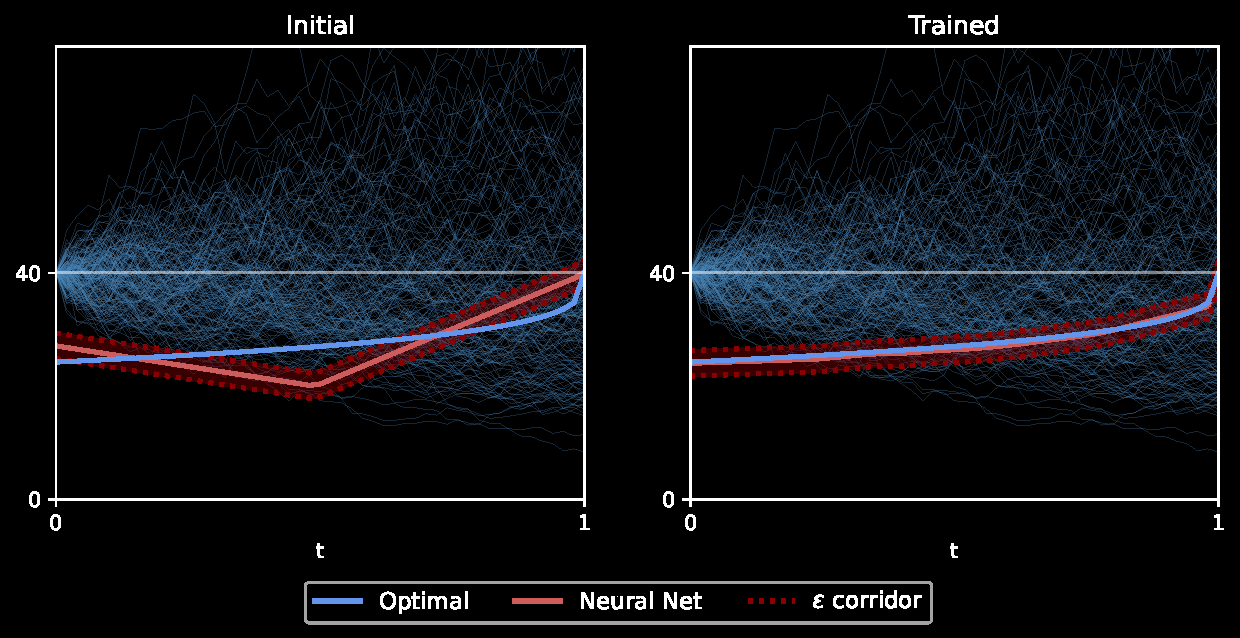
\includegraphics[scale=0.5]{FB/Figures/Bdry, lbda = 0.275.pdf}
    
%     \label{fig:putBS}
% \end{figure}

% \begin{figure}
%     \centering
%     \caption{Bermudan put option  ($N=50$),  Black-Scholes model.}
%     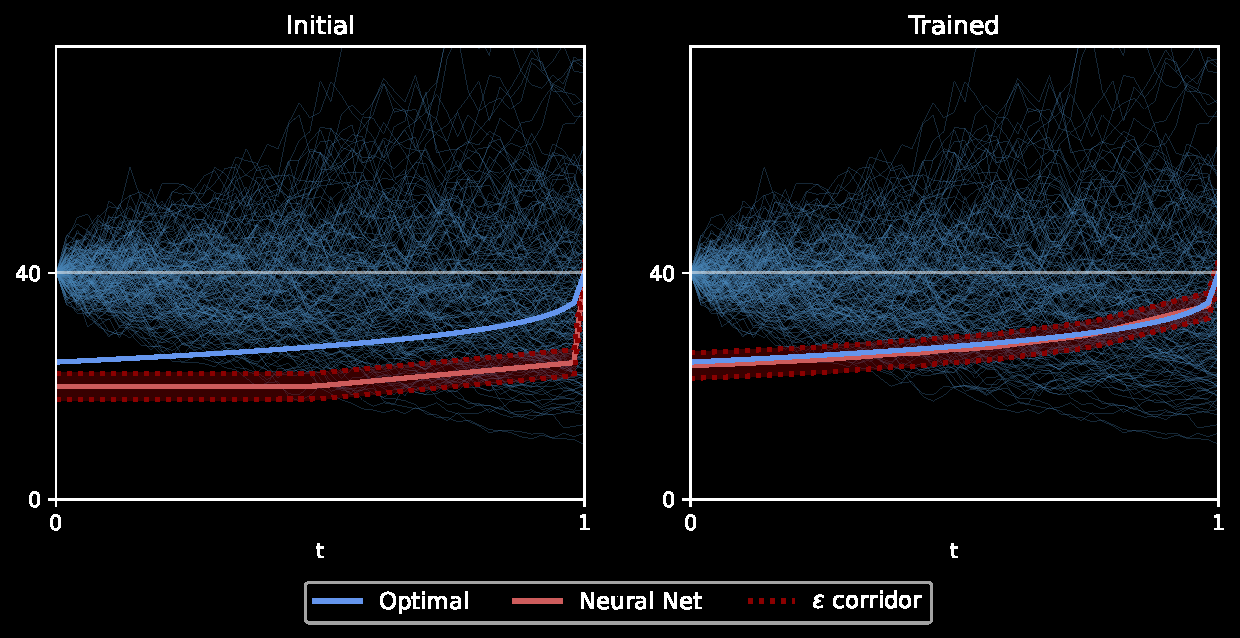
\includegraphics[scale=0.5]{FB/Figures/Bdry, lbda=0.275, mu=0.050, N=50.pdf}
    
%     \label{fig:putBS}
% \end{figure}

\begin{figure}
    \centering
    \caption{Exercise boundary (Bermudan put,  Black-Scholes model).}
    \includegraphics[scale=0.5]{FB/Figures/Bdry 2, lbda=0.275, mu=0.050, N=50.pdf}
    
    \label{fig:putBS}
\end{figure}

% \begin{figure}
%     \centering
%     \caption{Standard Bermudan put option, $N=50$, $\lambda = 0.15$.}
%     \includegraphics[scale=0.5]{FB/Figures/Bdry, lbda = 0.15.pdf}
    
%     \label{fig:put1D}
% \end{figure}
%$$v(t,s') $$  %$\calS = \prod_{t\in [0,T]} [f(t), \infty), $ for some threshold function $f:[0,T]\to [K,\infty)$.  

%Indeed, if $s\in \calS_t$ and $s' = \alpha(s') \ge \alpha(s) =s$, then 
%$$v(t,s') $$

\subsection{Put Option in the Heston Model}\label{sec:putHeston}

Consider the Bermudan put option from the previous section ($S_0 =K=40$, $T=1$, $N=50$) in the Heston model. Our goal is to see how stochastic volatility impacts the exercise boundary and  corresponding  price.   
 Let $m=1, \ k=0$ and assume the stock and factor dynamics
\begin{align*}
   \frac{dS_t}{S_t} &= (r-\delta)dt + \sqrt{\calV_t}\  dW_t, \\
   d\calV_t &= (\kappa(\bar{\nu}-\calV_t) - \gamma^{\Q}\calV_t)dt + \sigma_{\calV} \sqrt{\calV_t}\  d\tilde{W}_t, 
\end{align*}
with $\calV_0 = \nu_0 \in \R^2_+$ and $\frac{d\langle W, \tilde{W} \rangle_t}{dt} = \rho  \in  (-1,1)$. 
%Apart from the volatility, the parameters for $S$ are the same as in the previous section, that is $(S_0,K,r,\delta,T) = (40,40,6\%,0\%,40\%,1)$ and $N=50$. 
We choose the parameters
 $r = 6\%$, $\delta = 0\%$, $\kappa = 1$, $\nu_0 = \bar{\nu} = (40\%)^2$, $\gamma^{\Q} =0$, $\sigma_{\calV} =10\%$, and $\rho =-0.5$. In particular, 
the Feller condition $\kappa \,  \bar{\nu} \ge  \frac{\sigma_{\calV}^2}{2}$ is satisfied.  
%$(\kappa,\bar{\calV},\sigma_{\calV}) $ satisfies the Feller condition, i.e. $\kappa \bar{\calV}\ge  \frac{\sigma_{\calV}^2}{2}$. 
For a fair comparison,  we set the initial value and long term mean of $\calV$ equal to the Black-Scholes variance $\sigma^2$ from \cref{sec:putBS}.   Moreover, we use importance sampling with same Girsanov parameter, i.e. $\lambda \equiv \frac{r-\delta + 0.05}{\sigma}  = 0.275$.

As seen in \cref{ex:vanilla}, the threshold function 
depends on time $t$ and the spot variance $\calV_t =\nu$.  
When $\varphi$ is convex and bounded (which is the case here)   \citet{LambertonHeston} showed that the value function $v(t,x)$, $x=(s,\nu)$, is  non-decreasing in $\nu$ for all $t\in [0,T]$. Consequently, the map $\nu \mapsto f(t,\nu)$ is non-increasing. In figure..., it turns out that the same holds for the trained neural network $G(\cdot,\cdot;\theta^M)$. %Moreover, by construction of $f$,  we expect that the  segment $\{s\} \times [0,\nu]$ %\{(s,\gamma \nu) \ | \ \gamma \in [0,1]\}$ 
%is contained in $\calS_t$ whenever $(s,\nu) \in \calS_t$. 
Moreover, as $s \to v(t,s,\nu)$ is non-increasing for fixed $(t,\nu)$,  we expect that the  rectangle $[0,s]\times [0,\nu]$ %\{(s,\gamma \nu) \ | \ \gamma \in [0,1]\}$ 
is contained in $\calS_t$ whenever $(s,\nu) \in \calS_t$. This is confirmed in Figure. 

Table ... compares the price of the claim when the stopping decision exploit the spot variance and when it does not. We observe that the price obtained with the "blind" strategy is significantly lower. Interestingly, the neural network converges to the optimal boundary in the Black-Scholes model, as shown in Figure.... %obtained boundary $G(t;\theta)$ is the same as in the Black-Scholes model, as shown in Figure....  %As can be seen, the blind strategy is suboptimal. 

%For a sufficiently wide range $[\underline{\nu},\bar{\nu}]$ such that $\calV_t \in [\underline{\nu},\bar{\nu}]$ with high probability, we expect that the threshold process $f(t,\calV_t)$ lies between $f_{BS,\underline{\nu}}$. 

Figure .. displays a trajectory for $(X,\calV)$ together with the threshold process $G(\cdot,\calV;\theta^M)$. As can be seen, the threshold is typically above the Black-Scholes boundary when $\calV_t$ is below its mean ($0.16$) and vice versa. 
%The red curves $f_{BS,\underline{\nu}}$, $f_{BS,\bar{\nu}}$ are the exercize boundaries of the put option in the Black-Scholes model with volatility parameter and  $\sqrt{\underline{\nu}}$ , $\sqrt{\bar{\nu}}$, respectively. 

\begin{table}[ht]
  \centering
  \caption{Bermudan Put Option ($N=50$), Heston model.  
 }
  \begin{tabular}{|c| c| c| c| }
 \hline
  Threshold function &  Price&  Std& Runtime  \\
  \hline 
    $f(t,\nu)$ & 5.301 & 0.003 &  57.5 \\
  $f(t)$ & 5.281 & 0.003 &  57.5  \\
  \hline
\end{tabular}
\vspace{2mm}

\scriptsize{
\textit{Notes: The second and third column show the average and standard deviation of ten experiments, respectively.  }}
\label{tab:resultPutBS}
  \end{table}
  
\begin{figure}
    \centering
     \caption{Stopping and continuation regions (Bermudan put, Heston model).}
    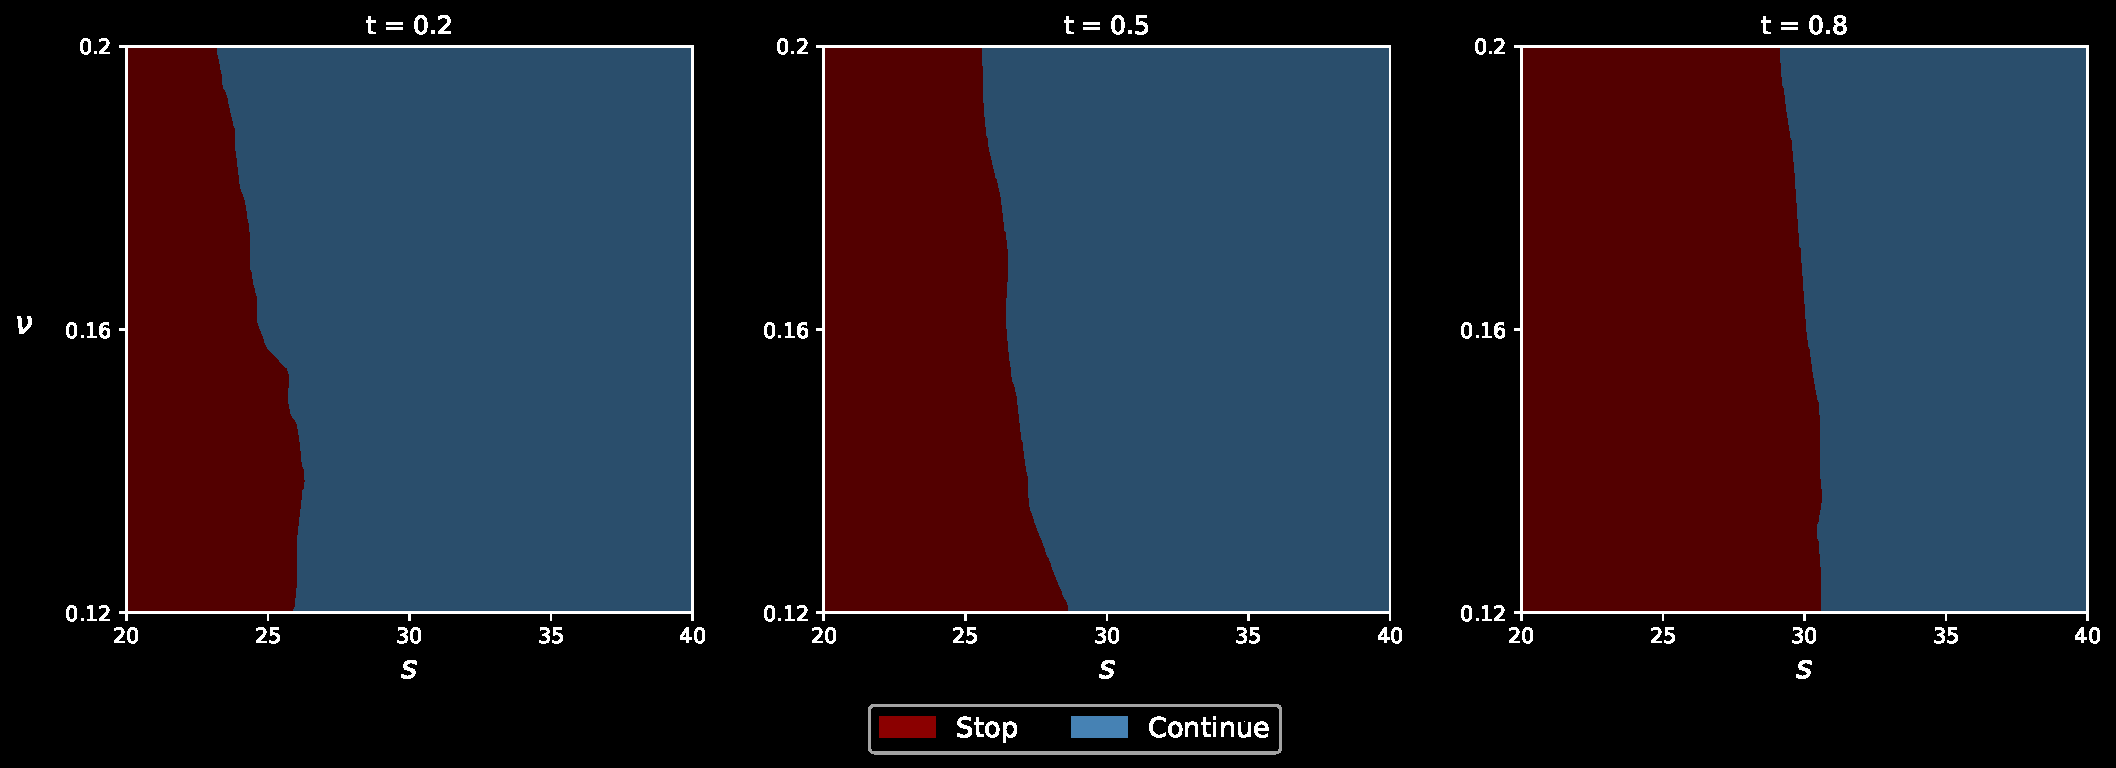
\includegraphics[scale = 0.42]{FB/Figures/2DPlotHeston.pdf}
    \label{fig:asymCall}
\end{figure}


%\bb{(+ Touzi's paper for SDEs with Lipschitz coefficients)}.




%The purpose of this section is to better understand the effect of stochastic volatility on the stopping region.  

%\subsection{Basket %Option}\label{sec:bskt}
%\subsection{Max Option}%\label{sec:maxCallSym}

\subsection{High-dimensional Max Option on Symmetric Assets}\label{sec:maxCallSym}
Let $\alpha(s) = \max_{i=1,...,d}s_i$, $\beta\equiv 0$, $\eta=1$ and consider the multi-dimensional Black-Scholes model with independent and symmetric assets, i.e. 
\begin{align}\label{eq:BSAsym}
    d S_t = \text{diag}(S_t) \left[ (r\mathds{1} - \delta)dt + \sigma dW_t\right],
\end{align}
where $W$ is Brownian motion in $\R^d$, $r \in \R ,\sigma > 0$ and $\delta \in \R_+^d$. We employ the parameters from Section of \cite{Becker2}, which are $s_0 =100 $, $r=5\%$, $\delta =10\%$ and $\sigma = 20 \%$. 

As both the payoff and assets are symmetric, it is easily shown that  $\calS_t$ is symmetric as well; see \cref{sec:symmetry}. This property can be exploited to reduce the dimension of our problem. Indeed, observe that it suffices to characterize the $t-$sections of the stopping region in the \textit{cone of ordered stocks}  
 $\calO = \{s\in \R_+^d \,|\, s_1 \geq \ldots \geq s_d\}$. We can therefore arrange $\Xi(S_t) = \frac{S_t}{\alpha(S_t)}\in [0,1]^d$ in decreasing order and give the outcome to $G(t,\cdot; \theta)$. If $\bar{S}_t \in \calO$ denotes the ordered version of $S_t$, then the last component of $\bar{S}_t$ are of little relevance to our stopping decision. 
 Indeed, over a short horizon, the maximum is  likely to be attained by the current best performing assets. %a stock having a high value today. 
 We can therefore set a cutoff $2 \le d' \ll d$ and feed the neural network with $(\frac{\bar{S}_{t,2}}{\alpha(S_t)},\ldots,\frac{\bar{S}_{t,d'}}{\alpha(S_t)})$ only.\footnote{Note that $\frac{\bar{S}_{t,1}}{\alpha(S_t)} \equiv 1$ is also removed from the neural network input as it doesn't carry any information.} Although one still needs to simulate $d$ assets, the size of the neural network can be significantly reduced, which in turn accelerates the training phase.  
 
 We illustrate this %In fact,  $\frac{\bar{S}_{t,1}}{\alpha(S_t)}$ is always equal to $1$ so it can be removed from the neural network input as well.} 
 
  %$-$ in decreasing order %The stopping region can be recovered by shuffling coordinates, namely $\calS_t = \bigcup_{\varsigma \in \calP_{\!d}} \varsigma(\calV_t)$ for $t\in[0,T]$. 

%$d=100$, cut-off:  $d \wedge 10$. 

\subsection{Max Option on $d=2$ Asymmetric Assets}\label{sec:maxCallAsym}
Consider the multi-dimensional Black-Scholes model, i.e. 
\begin{align}\label{eq:BSAsym}
    d S_t = \text{diag}(S_t) \left[ (r\mathds{1} - \delta)dt + \sigma dW_t\right],
\end{align}
where $W$ is Brownian motion in $\R^d$, $r \in \R ,\sigma > 0$ and $\delta \in \R_+^d$. 

Define the connected components $\calS^{(i)}_t = \calS_t \cap \{\alpha(s) = s_i\}$, $i=1,2$ and the involution   $\varsigma(s_1,s_2) := (s_2,s_1)$.  

\begin{proposition} Consider a max option on $d=2$ assets with $S$ having dynamics as in $\eqref{eq:BSAsym}$. IF $\delta_1 \ge \delta_2$, then $\varsigma(\calS^{(1)}_t) \subseteq \calS^{(2)}_t$. \rr{(to be verified numerically...)}
\end{proposition}

\begin{proof}
Let $t\in [0,T)$ and take any $\tau \in \calT_t$. Then, defining the event $B = \{S^{t,s_1}_{\tau,1} \ge  S^{t,s_2}_{\tau,2}\}$, this gives
\begin{align*}
    \E^{\Q}[D_{t,\tau} \varphi(S^{t,s}_{\tau}) ] &= \E^{\Q}[D_{t,\tau} (S^{t,s_1}_{\tau,1}-K)^+ \ \mathds{1}_{B} ] + \E^{\Q}[D_{t,\tau} (S^{t,s_2}_{\tau,2}-K)^+ \ \mathds{1}_{B^c} ]. 
\end{align*}
Since $\gamma := e^{(\delta_1-\delta_2)(\tau-t)} \le 1$, then  $\{\gamma S^{t,s_1}_{\tau,1} \ge  \gamma^{-1} S^{t,s_2}_{\tau,2}\} \subseteq B$. Moreover, note that $(\gamma S^{t,s_1}_{\tau,1},\gamma^{-1} S^{t,s_2}_{\tau,2}) \overset{d}{=} \varsigma(S^{t,\varsigma(s)}_{\tau})$. 
\begin{equation*}
    \E^{\Q}[D_{t,\tau} (S^{t,s_1}_{\tau,1}-K)^+ \ \mathds{1}_{B} ] \ge  \E^{\Q}\left[D_{t,\tau} (\gamma S^{t,s_1}_{\tau,1}-K)^+ \ \mathds{1}_{\{\gamma S^{t,s_1}_{\tau,1} \ge  \gamma^{-1} S^{t,s_2}_{\tau,2}\}} \right ] = \E^{\Q}[D_{t,\tau} ( S^{t,s_1}_{\tau,2}-K)^+ \ \mathds{1}_{B'} ],
\end{equation*}
with $B':= \{ S^{t,s_1}_{\tau,2} \ge  S^{t,s_2}_{\tau,1}\}$. On the other hand, note that $S^{t,s_2}_{\tau,2} \ge S^{t,s_1}_{\tau,1} \ge S^{t,s_2}_{\tau,1} $ on $B^c$. Hence, 
\begin{align*}
    \E^{\Q}[D_{t,\tau} (S^{t,s_2}_{\tau,2}-K)^+ \ \mathds{1}_{B^c} ] &\ge  \E^{\Q}[D_{t,\tau} (S^{t,s_2}_{\tau,1}-K)^+ \ \mathds{1}_{B^c} ]\\
    &\rr{\ge} \E^{\Q}[D_{t,\tau} (S^{t,s_2}_{\tau,1}-K)^+ \ \mathds{1}_{(B')^c} ].
\end{align*}
But $B^c \subseteq B$!

We would conclude: 
\begin{align*}
    \E^{\Q}[D_{t,\tau} \varphi(S^{t,s}_{\tau}) ] &\ge \E^{\Q}[D_{t,\tau} ( S^{t,s_1}_{\tau,2}-K)^+ \ \mathds{1}_{B'} ] + \E^{\Q}[D_{t,\tau} (S^{t,s_2}_{\tau,1}-K)^+ \ \mathds{1}_{(B')^c} ]\\ 
    &= \E^{\Q}[D_{t,\tau} \varphi(S^{t,\varsigma(s)}_{\tau}) ]. 
\end{align*}

...

To show: 
$$\E^{\Q}[ \varphi(S^{t,s}_{u}) ] \ge \E^{\Q}[ \varphi(S^{t,\varsigma(s)}_{u}) ], \quad \forall \ u \in [t,T].  $$
And multiply by $D_{t,u}$. 

E.g., use stochastic dominance $\alpha(S^{t,s}_{u}) \succ \alpha(S^{t,\varsigma(s)}_{u})$. And therefore, if $\varphi = \psi \circ \alpha$ with $\psi(a) \to 0$ as $a\to \infty$
\begin{align*}
    \E^{\Q}[\varphi(S^{t,s}_{u}) ] &= \int_0^{\infty} \psi(a) d\Q(\alpha(S^{t,s}_{u}) \le a) \\ 
    &=  - \int_0^{\infty} \Q(\alpha(S^{t,s}_{u}) \le a) d \psi(a) \\ 
    &\ge  - \int_0^{\infty} \Q(\alpha(S^{t,\varsigma(s)}_{u}) \le a) d \psi(a) \\ 
     &\ge  \E^{\Q}[\varphi(S^{t,\varsigma(s)}_{u}) ].
\end{align*}
 If needed,  use $\psi^N \uparrow \psi$  and the monotone convergence theorem.  
%$M^{t,s}_{u} \succ M^{t,\varsigma(s)}_{u} $, where $M^{t,s}_{u} = \alpha(S^{t,s}_{u})$. 
\end{proof}

\begin{figure}
    \centering
    \caption{Stopping and continuation regions (max option, $d=2$ assets, $T=3$).}
    \includegraphics[scale = 0.42]{FB/Figures/AsymMaxCall.pdf}
    \label{fig:asymCall}
    
    \scriptsize{
\textit{Notes: The light red region is the reflected image of $\calS_t^{(1)}$ through the diagonal, i.e. $\varsigma(\calS_t^{(1)})$.}} %This is to  illustrate that $\varsigma(\calS_t^{(1)}) \subseteq \calS_t^{(2)}$.  }}
\end{figure}

%\subsection{Spread Option}
%\subsection{Floating Strike Asian Option} \label{sec:Asian}
\subsection{Fixed Strike  Lookback Option} \label{sec:Lkbk}



%========= Section 5 ==========%
%\section{Numerical Experiments}

We now provide numerical evidence of the efficiency of our method. All the  experiments have been carried out  with Tensorflow 2.7  on a 2021 Macbook pro with 64GB unified memory and Apple M1 Max chip. The code is implemented in Python and run on CPU (10-core) only.  
Throughout the examples, we use the same neural network architecture and training parameters,  given  below:
\begin{enumerate}
\item The feedforward neural network consists of $2$ hidden layers, each having $20 + \text{dim}(\calE)$  nodes  with leaky rectified linear unit (Leaky ReLU) activation function. The output layer uses the standard rectified linear unit (ReLU)  activation. The  bias in the output layer can be used to set  an initial threshold level $\theta_0 \in \R_+$.     In other words, the  threshold function reads
$$G(t,\xi; \theta) = \left(\theta_0 + \theta_1^{\top} G_{-1}(t,\xi; \theta_{-1})\right)^+, \quad (\theta_{-1}, \theta_{0}, \theta_1) = \theta, $$ %, \quad \theta_1 \in \R^{50+\bar{d}}
where  $G_{-1}(t,\xi; \theta_{-1}) \in \R^{20+\bar{d}}$ is the value of the neural network before entering the output layer. From our observations, the algorithm is not sensitive to the initial bias, as long as it is set to a reasonable value.  For example, if the payoff is of the form   $\eqref{eq:payoff}$, we  choose $\theta_0=\frac{3K}{2}$,  $\theta_0=\frac{K}{2}$ for  calls 
and puts
,  respectively. 

\item The number of training iterations is set to $M=3,000$ and batch size to $B = 512$. 
    \item The learning rates $(\zeta_m)$ are obtained from the widely accepted Adam optimizer \cite{Kingma}.
    
    \item  
    If the payoff function is of the form
    $\eqref{eq:payoff}$ (which is the case in all the examples below), the fuzzy boundary width is chosen to be    
    $\epsilon_n = K \sqrt{\V^{\Q}[ \alpha(X^{t_{n-1},1}_{t_n})]}$, $t_n \in \calT_N$. 

     The strike $K$ takes account the scale of the payoff$-$and in turn, the threshold function$-$while  the second in $\epsilon_n$ reflects the typical variation 
     of the  process $\alpha(X)$ between exercise dates.  
\end{enumerate}
The initial price is computed using the sharp boundary and $J= 2^{22} = 4,194,304$ Monte Carlo simulations. 

\subsection{Put Option in the Black-Scholes Model} \label{sec:putBS}
Consider an ATM Bermudan put option ($\varphi(s) = (K-s)^+$) in the Black Scholes model. We take the same parameters as in  Section 4.3.1.2 of \cite{Becker2}, namely
$S_0=K=40$, $r = 6\%$, $\delta = 0\%$, $\sigma = 40\%$, with maturity $T=1$ and  $N=50$ exercise dates.  
As the stock price must reach low values to cross the boundary, we can use importance sampling to make the drift of $S-$which is positive under $\Q-$negative under an equivalent measure. We can for instance set $\lambda \equiv \frac{r-\delta + 0.05}{\sigma}  = 0.275$ so $S$ becomes a submartingale under $\Q^{\lambda}$ with $5\%$ negative drift. Notice that the fuzzy boundary width is approximately equal to $\epsilon = K\sigma \sqrt{T/N}$.  \cref{tab:resultPutBS} summarizes the result, in comparison with the value found by \citet{Becker1}. 

\begin{table}[ht]
  \centering
  \caption{Bermudan Put Option ($N=50$), Black-Scholes model.  
 }
  \begin{tabular}{|c| c| c| c| c|}
 \hline
     Price&  Std& Runtime  & Price in \cite{Becker2}\\
  \hline 
  5.308 & 0.003 &  57.5 & 5.311 \\
  \hline
\end{tabular}
\vspace{2mm}

\scriptsize{
\textit{Notes: The first and second column show the average and standard deviation of ten experiments, respectively. The third column is the average runtime (in seconds) per experiment for the training phase. }}
\label{tab:resultPutBS}
  \end{table}

Figure \ref{fig:putBS} displays the initial boundary (left chart) with the trained one (right chart) compared with the optimal boundary. The latter is obtained using a finite-difference scheme.  

\begin{figure}
    \centering
    \caption{Exercise boundary (Bermudan put,  Black-Scholes model).}
    \includegraphics[scale=0.5]{Figures/Bdry 2, lbda=0.275, mu=0.050, N=50.pdf}
    
    \label{fig:putBS}
\end{figure}

\subsection{Put Option in the Heston Model}\label{sec:putHeston}

Consider the Bermudan put option from the previous section ($S_0 =K=40$, $T=1$, $N=50$) in the Heston model. Our goal is to see how stochastic volatility impacts the exercise boundary and  corresponding  price.   
 Let $m=1, \ k=0$ and assume the stock and factor dynamics
\begin{align*}
   \frac{dS_t}{S_t} &= (r-\delta)dt + \sqrt{\calV_t}\  dW_t, \\
   d\calV_t &= (\kappa(\bar{\nu}-\calV_t) - \gamma^{\Q}\calV_t)dt + \sigma_{\calV} \sqrt{\calV_t}\  d\tilde{W}_t, 
\end{align*}
with $\calV_0 = \nu_0 \in \R^2_+$ and $\frac{d\langle W, \tilde{W} \rangle_t}{dt} = \rho  \in  (-1,1)$. 
We choose the parameters
 $r = 6\%$, $\delta = 0\%$, $\kappa = 1$, $\nu_0 = \bar{\nu} = (40\%)^2$, $\gamma^{\Q} =0$, $\sigma_{\calV} =10\%$, and $\rho =-0.5$. In particular, 
the Feller condition $\kappa \,  \bar{\nu} \ge  \frac{\sigma_{\calV}^2}{2}$ is satisfied.  
For a fair comparison,  we set the initial value and long term mean of $\calV$ equal to the Black-Scholes variance $\sigma^2$ from \cref{sec:putBS}.   Moreover, we use importance sampling with same Girsanov parameter, i.e. $\lambda \equiv \frac{r-\delta + 0.05}{\sigma}  = 0.275$.

As seen in \cref{ex:vanilla}, the threshold function 
depends on time $t$ and the spot variance $\calV_t =\nu$.  
When $\varphi$ is convex and bounded (which is the case here)   \citet{LambertonHeston} showed that the value function $v(t,x)$, $x=(s,\nu)$, is  non-decreasing in $\nu$ for all $t\in [0,T]$. Consequently, the map $\nu \mapsto f(t,\nu)$ is non-increasing. As can be seen in  \cref{fig:heston1}, it turns out that the same holds for the trained neural network $G(\cdot,\cdot;\theta^M)$.
Notice also that $\nu \mapsto f(t,\nu)$ becomes less steep as $t$ approaches maturity. This is line with the fact that the Vega  decreases over time until the option is exercised.  
As $s \to v(t,s,\nu)$ is non-increasing for fixed $(t,\nu)$,  we therefore expect that the  rectangle $[0,s]\times [0,\nu]$ 
is contained in $\calS_t$ whenever $(s,\nu) \in \calS_t$. This is confirmed in  \cref{fig:heston1}. 

 \cref{tab:resultPutHeston} compares the price of the claim when the stopping decision exploit the spot variance ($f = f(t,\nu)$) and when it does not ($f = f(t)$). We observe that the price obtained with the "blind" strategy is significantly lower. Interestingly, the neural network coincides with the optimal boundary in the Black-Scholes model. %, as shown in Figure \cref{fig:heston1}
 Finally, \cref{fig:heston2} displays a trajectory for $(X,\calV)$ together with the threshold process $G(\cdot,\calV;\theta^M)$. As can be seen, the threshold is typically below the Black-Scholes boundary when $\calV_t$ is above its mean $\bar{\nu} = 0.16$ and vice versa. 

\begin{table}[ht]
  \centering
  \caption{Price of a Bermudan Put Option in the Heston model. \bb{(std to be reduced)}  
 }
  \begin{tabular}{c c c c }
 \hline  \hline
  Threshold function &  Price&  Std& Runtime  \\
  \hline  \hline
    $f(t,\nu)$ & 5.295 & 0.005 &  57.5 \\
  $f(t)$ & 5.281 & 0.006 &  57.5  \\
  \hline
\end{tabular}
\vspace{2mm}

\scriptsize{
\textit{Notes: The second and third column show the average and standard deviation of ten experiments, respectively.  }}
\label{tab:resultPutHeston}
  \end{table}
  
\begin{figure}[t]
    \centering
     \caption{Stopping and continuation regions (Bermudan put, Heston model).}
    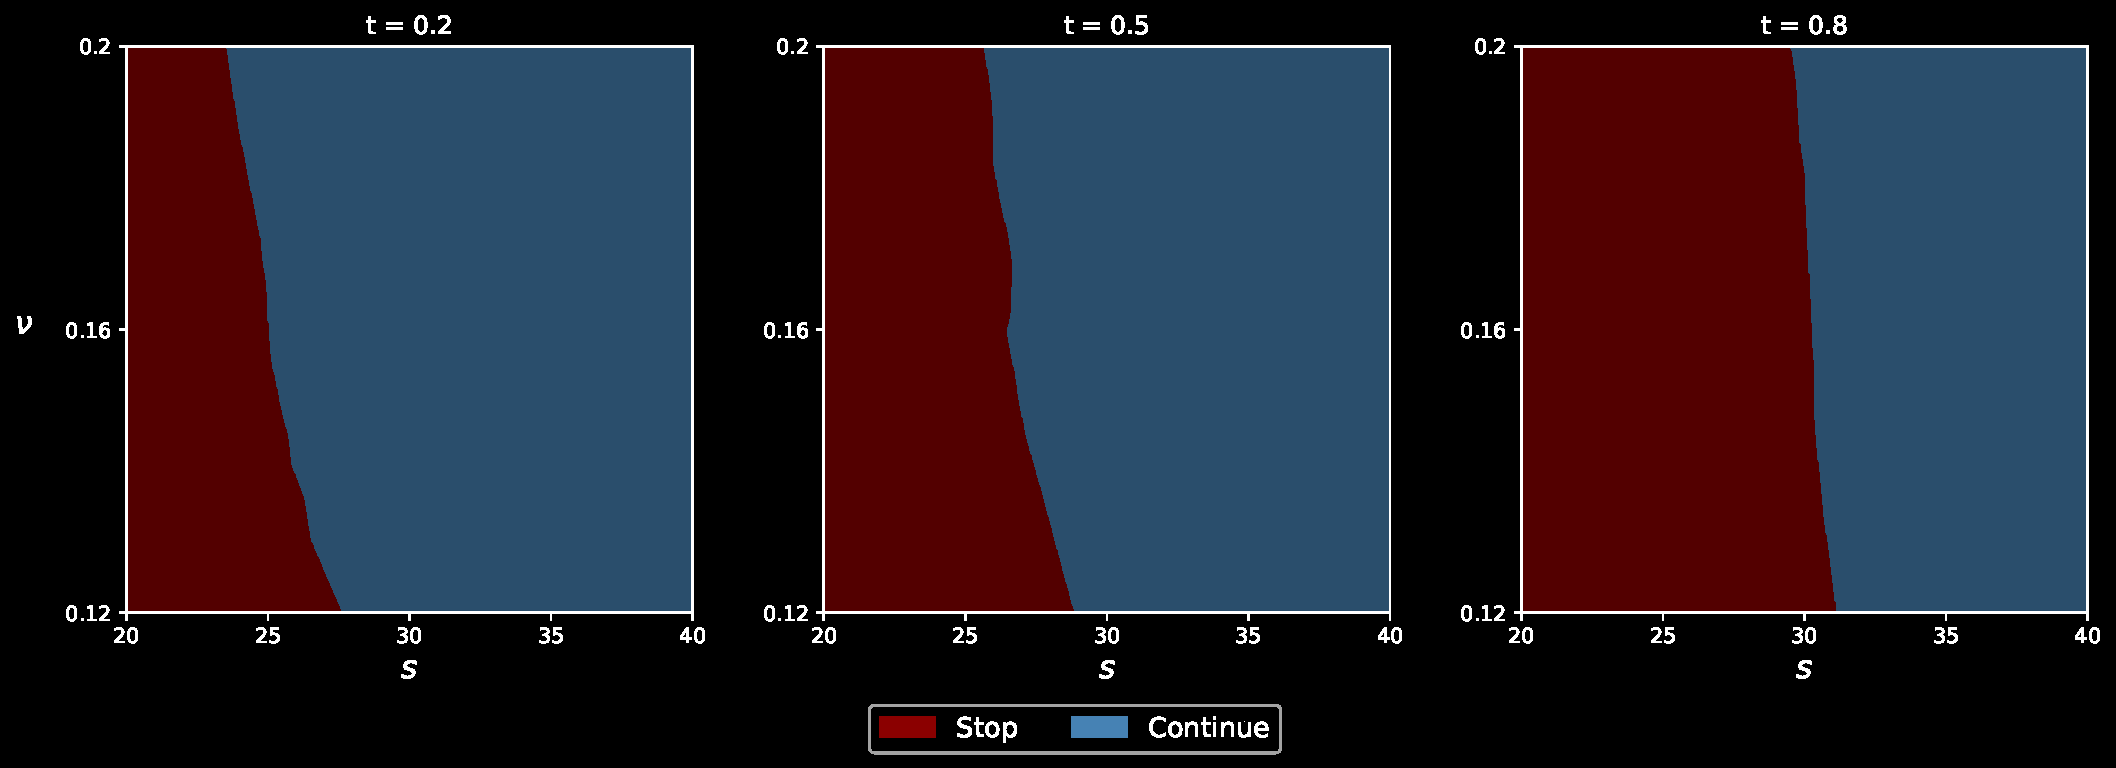
\includegraphics[scale = 0.42]{Figures/2DPlotHestonWide.pdf}
    \label{fig:heston1}
\end{figure}


\begin{figure}[t]
    \centering
     \caption{Stock price, variance and threshold process (Bermudan put, Heston model).}
    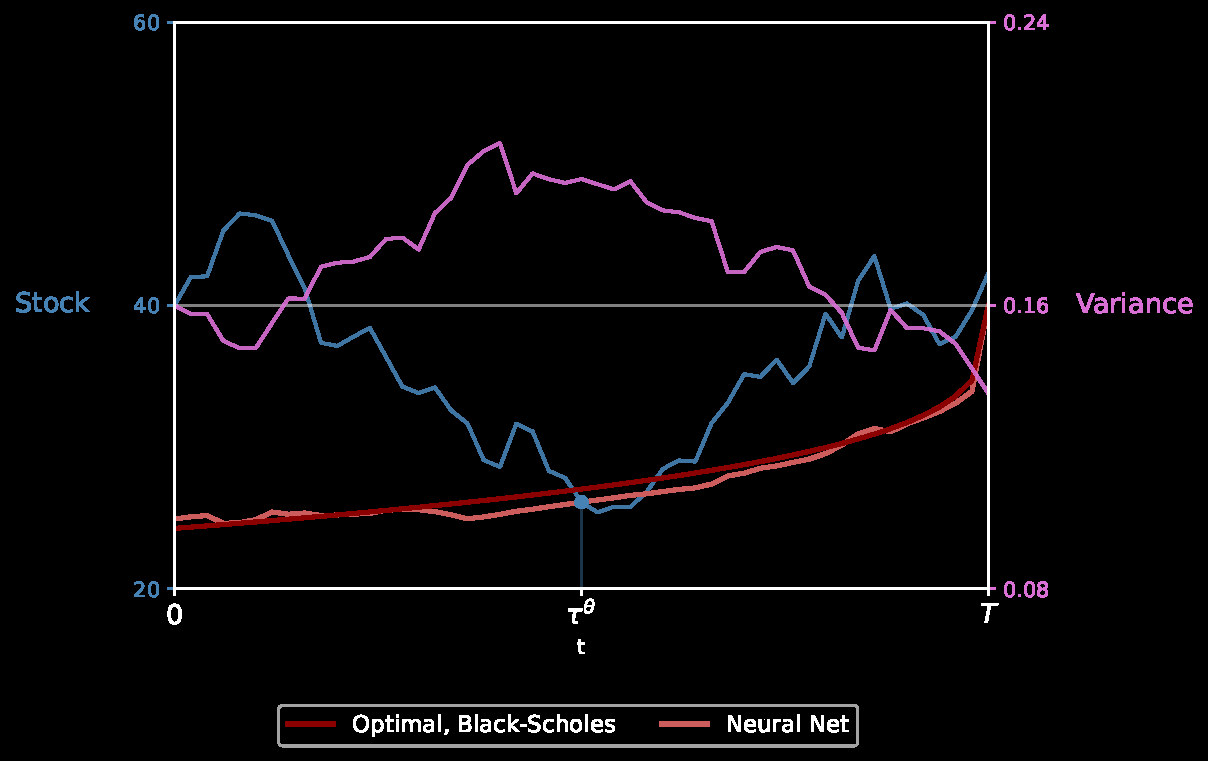
\includegraphics[scale = 0.42]{Figures/BdryHeston2.pdf}
    \label{fig:heston2}
\end{figure}


\subsection{High-dimensional Max Option on Symmetric Assets}\label{sec:maxCallSym}
Let $\alpha(s) = \max_{i=1,...,d}s_i$, $\beta\equiv 0$, $\eta=1$ and consider the multi-dimensional Black-Scholes model with independent and symmetric assets, i.e. 
\begin{align}\label{eq:BSAsym}
    d S_t = \text{diag}(S_t) \left[ (r\mathds{1} - \delta)dt + \sigma dW_t\right],
\end{align}
where $W$ is Brownian motion in $\R^d$, $r \in \R ,\sigma > 0$ and $\delta \in \R_+^d$. We employ the parameters from Section 4.4.1 in \cite{Becker2}, which are $s_0 =100 $, $r=5\%$, $\delta =10\%$ and $\sigma = 20 \%$. 

As both the payoff and assets are symmetric, it is easily shown that  $\calS_t$ is symmetric as well; see \cref{sec:symmetry}. This property can be exploited to reduce the dimension of our problem. Indeed, observe that it suffices to characterize the $t-$sections of the stopping region in the \textit{cone of ordered stocks}  
 $\calO = \{s\in \R_+^d \,|\, s_1 \geq \ldots \geq s_d\}$. We can therefore arrange $\Xi(S_t) = \frac{S_t}{\alpha(S_t)}\in [0,1]^d$ in decreasing order and give the outcome to $G(t,\cdot; \theta)$. If $\bar{S}_t \in \calO$ denotes the ordered version of $S_t$, then the last component of $\bar{S}_t$ are of little relevance to our stopping decision. 
 Indeed, over a short horizon, the maximum is  likely to be attained by the current best performing assets. %a stock having a high value today. 
 We can therefore set a cutoff $2 \le d' \ll d$ and feed the neural network with $(\frac{\bar{S}_{t,2}}{\alpha(S_t)},\ldots,\frac{\bar{S}_{t,d'}}{\alpha(S_t)})$ only.\footnote{Note that $\frac{\bar{S}_{t,1}}{\alpha(S_t)} \equiv 1$ is also removed from the neural network input as it doesn't carry any information.} Although one still needs to simulate $d$ assets, the size of the neural network can be significantly reduced, which in turn accelerates the training phase.  
 
 We illustrate this argument with $d=20$ assets and a cutoff of $d'=5$. 



\begin{table}[ht]
\caption{Max Option on $d \in\{5,10,20,50\}$ symmetric assetes}
\label{lab:symMaxOpt}
  \centering
  \begin{tabular}{ c c c c c c}
 \hline  \hline
   $d$ &  {\bf{Price}}&  {\bf{Std}}&  {\bf{Price in \cite{Becker2}}}&
    {\bf{Max Price}} & {\bf{Its Std}}\\
  \hline \hline
  5   & 26.1295 &  0.0095 & 26.147 &26.1506 &  0.0094 \\
 %\hline
  10   & 38.2735 &  0.0538 & 38.272 & 38.3351 &  0.0089  \\
    20   &  &   & 51.572 &  &    \\
 %\hline
  50  &  &   & 69.572  &  &   \\
 \hline
\end{tabular}

\vspace{2mm
}
 \scriptsize{
\textit{Notes: The second and third column show the average and standard deviation of ten experiments, respectively.  }}
  \end{table}
  
\subsection{Max Option on $d=2$ Asymmetric Assets}\label{sec:maxCallAsym}
Consider the multi-dimensional Black-Scholes model, i.e. 
\begin{align}\label{eq:BSAsym}
    d S_t = \text{diag}(S_t) \left[ (r\mathds{1} - \delta)dt + \sigma dW_t\right],
\end{align}
where $W$ is Brownian motion in $\R^d$, $r \in \R ,\sigma > 0$ and $\delta \in \R_+^d$. 
Define the connected components $\calS^{(i)}_t = \calS_t \cap \{\alpha(s) = s_i\}$, $i=1,2$ and the involution   $\varsigma(s_1,s_2) := (s_2,s_1)$.  

\begin{proposition} Consider a max option on $d=2$ assets with $S$ having dynamics as in $\eqref{eq:BSAsym}$. If $\delta_1 \le \delta_2$, then $\varsigma(\calS^{(1)}_t) \subseteq \calS^{(2)}_t$. \rr{(to be verified numerically...)}
\end{proposition}

\begin{proof} (\bb{attempts...})
Let $t\in [0,T)$ and take any $\tau \in \calT_t$. Then, defining the event $B = \{S^{t,s_1}_{\tau,1} \ge  S^{t,s_2}_{\tau,2}\}$, this gives
\begin{align*}
    \E^{\Q}[D_{t,\tau} \varphi(S^{t,s}_{\tau}) ] &= \E^{\Q}[D_{t,\tau} (S^{t,s_1}_{\tau,1}-K)^+ \ \mathds{1}_{B} ] + \E^{\Q}[D_{t,\tau} (S^{t,s_2}_{\tau,2}-K)^+ \ \mathds{1}_{B^c} ]. 
\end{align*}
Since $\gamma := e^{(\delta_1-\delta_2)(\tau-t)} \le 1$, then  $\{\gamma S^{t,s_1}_{\tau,1} \ge  \gamma^{-1} S^{t,s_2}_{\tau,2}\} \subseteq B$. Moreover, note that $(\gamma S^{t,s_1}_{\tau,1},\gamma^{-1} S^{t,s_2}_{\tau,2}) \overset{d}{=} \varsigma(S^{t,\varsigma(s)}_{\tau})$. 
\begin{equation*}
    \E^{\Q}[D_{t,\tau} (S^{t,s_1}_{\tau,1}-K)^+ \ \mathds{1}_{B} ] \ge  \E^{\Q}\left[D_{t,\tau} (\gamma S^{t,s_1}_{\tau,1}-K)^+ \ \mathds{1}_{\{\gamma S^{t,s_1}_{\tau,1} \ge  \gamma^{-1} S^{t,s_2}_{\tau,2}\}} \right ] = \E^{\Q}[D_{t,\tau} ( S^{t,s_1}_{\tau,2}-K)^+ \ \mathds{1}_{B'} ],
\end{equation*}
with $B':= \{ S^{t,s_1}_{\tau,2} \ge  S^{t,s_2}_{\tau,1}\}$. On the other hand, note that $S^{t,s_2}_{\tau,2} \ge S^{t,s_1}_{\tau,1} \ge S^{t,s_2}_{\tau,1} $ on $B^c$. Hence, 
\begin{align*}
    \E^{\Q}[D_{t,\tau} (S^{t,s_2}_{\tau,2}-K)^+ \ \mathds{1}_{B^c} ] &\ge  \E^{\Q}[D_{t,\tau} (S^{t,s_2}_{\tau,1}-K)^+ \ \mathds{1}_{B^c} ]\\
    &\rr{\ge} \E^{\Q}[D_{t,\tau} (S^{t,s_2}_{\tau,1}-K)^+ \ \mathds{1}_{(B')^c} ].
\end{align*}
But $B^c \subseteq B$!

We would conclude: 
\begin{align*}
    \E^{\Q}[D_{t,\tau} \varphi(S^{t,s}_{\tau}) ] &\ge \E^{\Q}[D_{t,\tau} ( S^{t,s_1}_{\tau,2}-K)^+ \ \mathds{1}_{B'} ] + \E^{\Q}[D_{t,\tau} (S^{t,s_2}_{\tau,1}-K)^+ \ \mathds{1}_{(B')^c} ]\\ 
    &= \E^{\Q}[D_{t,\tau} \varphi(S^{t,\varsigma(s)}_{\tau}) ]. 
\end{align*}

...

To show: 
$$\E^{\Q}[ \varphi(S^{t,s}_{u}) ] \ge \E^{\Q}[ \varphi(S^{t,\varsigma(s)}_{u}) ], \quad \forall \ u \in [t,T].  $$
And multiply by $D_{t,u}$. 

E.g., use stochastic dominance $\alpha(S^{t,s}_{u}) \succ \alpha(S^{t,\varsigma(s)}_{u})$. And therefore, if $\varphi = \psi \circ \alpha$ with $\psi(a) \to 0$ as $a\to \infty$
\begin{align*}
    \E^{\Q}[\varphi(S^{t,s}_{u}) ] &= \int_0^{\infty} \psi(a) d\Q(\alpha(S^{t,s}_{u}) \le a) \\ 
    &=  - \int_0^{\infty} \Q(\alpha(S^{t,s}_{u}) \le a) d \psi(a) \\ 
    &\ge  - \int_0^{\infty} \Q(\alpha(S^{t,\varsigma(s)}_{u}) \le a) d \psi(a) \\ 
     &\ge  \E^{\Q}[\varphi(S^{t,\varsigma(s)}_{u}) ].
\end{align*}
 If needed,  use $\psi^N \uparrow \psi$  and the monotone convergence theorem.  
%$M^{t,s}_{u} \succ M^{t,\varsigma(s)}_{u} $, where $M^{t,s}_{u} = \alpha(S^{t,s}_{u})$. 
\end{proof}

\begin{figure}
    \centering
    \caption{Stopping and continuation regions (max option, $d=2$ assets, $T=3$).}
    \includegraphics[scale = 0.42]{Figures/AsymMaxCall.pdf}
    \label{fig:asymCall}
    
    \scriptsize{
\textit{Notes: The light red region is the reflected image of $\calS_t^{(1)}$ through the diagonal, i.e. $\varsigma(\calS_t^{(1)})$.}} %This is to  illustrate that $\varsigma(\calS_t^{(1)}) \subseteq \calS_t^{(2)}$.  }}
\end{figure}

%\subsection{Spread Option}
%\subsection{Floating Strike Asian Option} \label{sec:Asian}
\subsection{Fixed Strike  Lookback Option} \label{sec:Lkbk}



%======= Conclusion ===========%
\section*{Conclusion}

%\appendix 
\setcounter{section}{0}
\renewcommand*{\thesection}{\arabic{chapter}.\Alph{section}}

\section{Some Properties of the Stopping Region}
We briefly discuss some properties of the $t-$sections $\calS_t$ which can be relevant for the parametrization of the free boundary. 

\subsubsection{Symmetry}\label{sec:symmetry}

Many multi-asset, path-independent derivatives  present a type of symmetry in their payoff; see  \cref{ex:bskt} and \ref{ex:max}. Under certain conditions, this will carry over to the  stopping region. 
We assume $X=S$ throughout and  first recall the definition of symmetric functions. 

\begin{definition}
  A  function $\varphi: \R_+^d \to \R$ is called  \textit{symmetric} if it is invariant under permutation of its argument. Put differently, it must satisfy
    $$\varphi \circ \varsigma = \varphi, \quad \forall \ \varsigma \in \calP_{\! d} :=  \{\varsigma: \R^d_+ \mapsto \R^d_+ \, |\, \{s'_1,\ldots,s'_d\}=\{s_1,\ldots,s_d\}, \ s' = \varsigma(s) \}.$$%\{\varsigma: \R^d_+ \mapsto \R^d_+ \, |\, \varsigma(s)=(s_{i_1},...,s_{i_d}), \{i_1,...,i_d\} = \{1,...,d\} \}
   %with the group of permutations  $\calP_{\! d} =  \{\varsigma: \R^d_+ \mapsto \R^d_+ \, |\, \varsigma(s)=(s_{i_1},...,s_{i_d}), \{i_1,...,i_d\} = \{1,...,d\} \}.$
    %where $\calP_{\! d}$ is the group of permutations, 
    %$$\calP_d = \{\varsigma: \R^d_+ \mapsto \R^d_+ \, |\, \varsigma(s)=(s_{i_1},...,s_{i_d}), \{i_1,...,i_d\} = \{1,...,d\} \}.$$
\end{definition}

We also make the following distributional assumption on the stock prices.

\begin{asm}\label{asm: id} For all $(t,s)\in [0,T]\times \R_+^d$, the law of the forward-starting process $S^{t,s}$  is invariant under permutation, that is
    \begin{equation}\label{eq:id}
        \varsigma(S^{t,s}) \circ \Q = S^{t,\varsigma(s)} \circ  \Q, \quad \forall \ \varsigma \in \calP_{\!d}.
    \end{equation}
    % \begin{equation}
    %     \Q \circ (S^{t,s})^{-1} \circ \varsigma^{-1}  = \Q \circ (S^{t,\varsigma(s)})^{-1},
    % \end{equation}

    %The stock prices are identically distributed when starting at the same point, i.e. 
    %$$ \sigma(S^{t,\mathds{1}})  \circ \Pb = S^{t,\mathds{1}}  \circ \Pb \quad \forall \,\sigma \in \calP_d.$$
\end{asm}

Note that when Assumption \ref{asm: id} fails to hold,  the stopping region is in general not symmetric, regardless of the symmetry of $\varphi$; see \cref{sec:maxCallAsym}. 
The following result is now immediate.
\begin{proposition}
\label{prop:sym} Let $\varphi$
 be a symmetric payoff. If Assumption \ref{asm: id} holds, then the $t-$sections of the stopping region associated to $\varphi$ satisfy
$\varsigma(\calS_t)= \calS_t$ whatever $ \varsigma \in \calP_{\!d}$.
\end{proposition}
\begin{proof} Fix $t \in [0,T]$ and an arbitrary permutation $\varsigma \in \calP_d$. As $\varphi$ is symmetric, we show equivalently that $v(t,\cdot) \circ \varsigma =v(t,\cdot)$ with $v$ the associated value function. 
Given $\tau \in \calT_{\!t}$, we have
\begin{align*}\label{eq:proofSym}
    \E^{\Q}[\varphi(\tau,S^{t,s}_\tau)] =  \E^{\Q}[\varphi(\tau,\varsigma(S^{t,s}_\tau))] \
    \overset{\eqref{eq:id}}{=} \ \E^{\Q}[\varphi(\tau,S^{t,\varsigma(s)}_\tau)].
\end{align*}
Taking the supremum over all stopping times %on both sides %of $\eqref{eq:proofSym}$ 
yields the claim.
\end{proof}
Under the hypotheses of Proposition \ref{prop:sym}, it is sufficient to characterize the $t-$sections,  
$$\calV_t= \calS_t \cap \calO, \quad t \in [0,T], $$ where $\calO = \{s\in \R_+^d \,|\, s_1 \geq \ldots \geq s_d\}$ denotes the \textit{cone of ordered stocks}. The stopping region can be recovered by shuffling coordinates, namely $\calS_t = \bigcup_{\varsigma \in \calP_{\!d}} \varsigma(\calV_t)$ for $t\in[0,T]$.\footnote{Indeed, if $s\in  \bigcup_{\varsigma \in \calP_{\!d}} \varsigma(\calV_t)$, then $s=\varsigma(s')$ for some pair $(\varsigma,s') \in \calP_d \times \calV_t$. Hence 
$s \in \calS_t$ thanks to Proposition \ref{prop:sym}. Conversely for $s\in \calS_t$, there exists $\bar{\varsigma} \in \calP_d $ s.t. $s':=\bar{\varsigma}(s) \in \calO$ ($\bar{\varsigma}$ simply sorts  $s$ in non-increasing order). Proposition \ref{prop:sym} implies that $s' \in \calS_t$, which in turn gives   $ s' \in \calV_t$ and $s = \bar{\varsigma}^{\ -1}(s') \in \bigcup_{\varsigma \in \calP_d} \varsigma(\calV_t)$.} 
This fragmentation present benefits from a computational standpoint; see \cref{sec:maxCallSym}. 

 %Indeed, consider a max-call option on $d=2$ assets in the Black-Scholes model with same volatility but different dividend rates. Then \bb{...}
\subsubsection{Convexity}
Knowing topological properties of the unknown stopping region can help to characterize it more efficiently. We here focus on convexity. As the stopping region may not be connected (see \cref{ex:max}), we aim at determining when each connected component is convex.  We start off with some assumptions. 

\begin{asm}\label{asm:convlin}
$x \mapsto \varphi(x)$ is convex on $\calX$ and affine within each connected component of  $\calS_t$. 
\end{asm}

% Note that Assumption \ref{asm: convlin} is fulfilled by all payoffs from Section \ref{sec:examples}. Indeed, this is immediate when the functions $\alpha,  \beta$ in $\eqref{eq:payoff}$ are affine and for the max-option, the payoff is the positive part of a non-decreasing convex function, hence convex.   
We also need the following condition on $X$, which holds for instance for arithmetic and geometric Brownian motions. 
\begin{asm} \label{asm:affine}
    Given $0\le t \le u \le T$, the stochastic flow $x \mapsto X_u^{t,x}$  is an affine function.
\end{asm}

If both \cref{asm:scale} and  \ref{asm:affine}  hold, then necessarily $X_u^{t,x} = x \odot X_u^{t,\mathds{1}}$ so  the process is of "geometric" type. This leads us to the following result. 

\begin{proposition}
Under \cref{asm:convlin} and \ref{asm:affine}, $\calS_t$ is convex within each connected component.
\end{proposition}

\begin{proof}
Let $x,x'\in \calS_t$ belonging to the same connected component and  $\tilde{x}=\gamma x + (1-\gamma)x'$ for $\gamma \in [0,1]$. Then for all $\tau \in \calT_t$,
\begin{align*}
\E^{\Q}[D_{t,\tau}\varphi(X^{t,\tilde{x}}_\tau)] &=%\overset{\ref{asm:affine}}{=} 
\E^{\Q}[D_{t,\tau} \varphi(\gamma X^{t,x}_\tau + (1-\gamma) X^{t,x'}_\tau)]\\
    &\leq%\overset{\ref{asm:convlin}}{\leq}
    \gamma \E^{\Q}[D_{t,\tau}\varphi(X^{t,x}_\tau)]
    +
    (1-\gamma)\E^{\Q}[D_{t,\tau}\varphi(X^{t,x'}_\tau)]\\
    &\leq \gamma \varphi(x) + (1-\gamma) \varphi(x')\\
    &= %\overset{\ref{asm:convlin}}{=}
    \varphi(\tilde{x}).
\end{align*}
\end{proof}
Working with convex stopping regions is convenient as a continuum of stopping points can be deduced solely based on a few elements of $\calS_t$. Indeed, if we identify $x^{1},...,x^{J}$ as belonging to  $\calS_t$ %using the neural net $\Phi(\cdot;\theta)$,
, then   $\text{conv}(\{x^{1},...,x^{J}\}) \subseteq \calS_t$ as well.
%\subsection{Other properties of $\calS_t$}
\subsubsection{Monotonicity in Time}

%This property is valid for path-dedenpendent payoffs as well. 

\begin{proposition}\label{prop:monot}
Suppose that  $X$ and $D$ are stationary, that is $   
        X_u^{t,x} \circ \Q = X_{u-t}^{0,x} \circ  \Q \ $  and $D_{t,u} = D_{0,t-u}$ for every $t \le u $. 
Then the exercise boundary  expands over time, i.e. 
$ \calS_t \subseteq \calS_{t'}$ for all $t \le  t' $.

\end{proposition}
\begin{proof}
Take $t,t'\in [0,T]$ such that $\delta t := t'-t \ge 0$. %\footnote{The shift operator can be used, too.} 
 For  $\tau \in \calT_{t'}$, we have
\begin{align*}
    \E^{\Q}[D_{t',\tau}\varphi(X^{t',x}_{\tau})] &= \E^{\Q}[D_{t,\tau - \delta t }\varphi(X^{t,x}_{\tau - \delta t})] \le v(t,x), 
\end{align*}
as $\tau - \delta t \in \calT_t \cap \ [t,T-\delta t] \subseteq \calT_t$. If  $x\in \calS_t$, this gives   
$\E^{\Q}[D_{t',\tau}\varphi(X^{t',x}_{\tau})] \le  \varphi(x)$ for all $ \tau \in \calT_{t'} $ so  $x \in \calS_{t'}$ as claimed. 
\end{proof}

% \begin{corollary}
% \label{cor:monot} Let $\xi \in \calE$ and $f$  as  in $\eqref{eq:thres}$. Then $t \mapsto f(t,\xi)$  is non-increasing.
% \end{corollary}
% \begin{proof}  Fix $\xi \in \calE$ and suppose that $a \in \calA_{t,\xi}$, i.e. $A^{-1}(a,\xi) \in \calS_t$. If $t' \ge t$, then $A^{-1}(a,\xi) \in \calS_{t'}$ as well from which we conclude that $\calA_{t,\xi} \subseteq \calA_{t',\xi}$. Thus $f(t',\xi) = \inf \calA_{t',\xi} \le \inf \calA_{t,\xi} = f(t,\xi)$. 
% \end{proof}

% \begin{remark}
% If we  assume instead that the homeomorphism satisfies
% $$\left [ s\in \calS_t,\,  \Xi(s)=\Xi(s'), \,  \alpha(s')\geq \alpha(s) \right]  \Longrightarrow s'\in \calS_t,$$ (e.g. for a call-type payoff), then 
% $$f(t,x)= \inf \{a \in \R \, |\, A^{-1}(a,x) \in \calS_t\},$$
% and Corollary \ref{cor:monot} implies  that $t\mapsto f(t,x)$ is non-increasing.
% \end{remark}

\subsubsection{Scale Invariance}

Suppose that the payoff involves a parameter $K>0$, e.g. the strike of a vanilla option.  We write $\varphi_K$, $v_K$, $\calS_{t,K}$ and $f_K$ with the obvious notations. 
\begin{asm} \label{asm:homo}
The payoff is homogeneous in the sense that $\varphi_{K\gamma}(\gamma x)=\gamma \varphi_{K}(x)$, $\forall \  \gamma>0$. 
\end{asm}

\begin{proposition}\label{lem:homogen}
If  \cref{asm:scale} and \ref{asm:homo} hold,
then 
$\calS_{t,K}=K\calS_{t,1}:= \{Ks \,|\, s \in \calS_{t,1}\}.$
\end{proposition}
\begin{proof}
If $\varphi_K$ is homogeneous, then for all $t\in [0,T]$ and $\tau \in \calT_t$,
$$ \E[D_{t,\tau}\varphi_K(X^{t,x}_{\tau})] = \E[D_{t,\tau}\varphi_K(K X^{t,x/K}_{\tau})] =  K \E[D_{t,\tau} \varphi_1(X^{t,x/K}_{\tau})].$$
Thus $v_K(t,x) = K v(t,x/K)$, which finally gives 
\begin{align*}
    x \in \calS_{t,K} \Longleftrightarrow \varphi_K(x) = v_K(t,x)
    \Longleftrightarrow \varphi_1(x/K) = v_1(t,x/K)
    \Longleftrightarrow x \in K\calS_{t,1}.
\end{align*}
\end{proof}

% \begin{corollary}
% Suppose that the inverse function $A^{-1}: \R \times \calR \mapsto \R_+^d$ is homogeneous of degree $1$, i.e. $A^{-1}(a\gamma,x\gamma) = \gamma A^{-1}(a,x)$, $\gamma>0$. Then the exercise boundary satisfies
% $$f_K(t,x)= K \, f_1(t,x/K), \quad x \in \calR.$$
% \end{corollary}

% \begin{proof}
% Lemma \ref{lem:homogen} and the definition of $f_K$ directly give
% \begin{align*}
%     f_K(t,x) &= \sup \{a \in \R \,|\, A^{-1}(a,x) \in \calS_{t,K} \}\\
% &= \sup \{a \in \R \,|\, A^{-1}(a,x) \in K\calS_{t,1} \}\\
% &= \sup \left \{a \in \R \,|\, A^{-1}(a/K,x/K) \in \calS_{t,1}\right \}\\
% &= K f_1(t,x/K).
% \end{align*}

% \end{proof}

% \begin{example}
% Consider a basket
% option. A valid homeomorphism is  $A=(\alpha,\Xi)$ with  $$\alpha(s) = \frac{1}{d} \sum_{i=1}^d s_i, \quad \Xi(s) = s - \alpha(s).$$
% Then the inverse map $A^{-1}(a,x)=a+x$ is clearly homogeneous and the same therefore holds for $f_K$.
% \end{example}

% \begin{corollary}
% If the inverse map satisfies $A^{-1}(a\gamma,x) = \gamma A^{-1}(a,x)$, $\gamma>0$, then 
% $$f_K(t,x)= K \, f_1(t,x), \quad x \in \calR.$$
% \end{corollary}

% \begin{proof}
% Same argument as in the previous Corollary.
% \end{proof}

% \begin{example}
% For a max option, take $A=(\alpha,\Xi)$ with  $$\alpha(s) = s_1, \quad \Xi(s) = \frac{s}{s_1}.$$
% Then  $A^{-1}(a,x)=a x$ clearly verifies $A^{-1}(a\gamma,x) = \gamma A^{-1}(a,x)$ and thus $f_K(t,x)= K \, f_1(t,x) \; \forall  x \in \calR.$ Notice that this also holds for spread options.
% \end{example}

% \begin{corollary}
% The exercise boundary of American, single asset, vanilla options is homogeneous, i.e.
% $$f_K(t)= K \, f_1(t).$$
% \end{corollary}
% \begin{proof} It is clear that vanilla payoffs fulfill assumption \ref{asm:homo}.
% For  American puts, we get
% $$f_K(t) = \sup  \calS_{t,K} = \sup  K  \calS_{t,1} = K \sup \calS_{t,1} = K \, f_1(t).$$
% For  American calls, use infima instead.

\renewcommand*{\thesection}{\arabic{chapter}.\arabic{section}}

%\bibliography{FB/ref.bib}


%\chapter{Path-Dependent Claims: Projection and Fast Pricing}

The pricing of exotic 
options remains a difficult task in quantitative finance. The main challenge is to find an adequate trade-off between pricing accuracy and fast computation. Efficient techniques such as finite difference \cite{Schwartz} or the fast Fourier transform \cite{Carr} are in general not applicable to path-dependent payoffs. Practitioners are often forced to turn to  standard Monte Carlo methods, despite being  slow. 
Therefore, researchers have come up with novel ideas over the years to tackle this issue.   
Recently, \citet{Hull} have employed deep learning to price vanilla and exotic options in a non-parametric manner while \citet{Szpruch,LyonsNum}
showed the benefits of the path signature  to project exotic payoffs in a nonlinear way. 

In this chapter, we move away from  prevailing machine learning methods and bring a classical tool  back into play: the Karhunen-Loève (KL) expansion \cite{Karhunen, Loeve}. The latter provides an  orthogonal decomposition of stochastic processes that is optimal in the $L^2(\Q \otimes dt)$ sense. %Many applications have been promising to approximate Gaussian process 
The theory has been widely applied to Gaussian processes \cite{Ghanem,Solin}  and  recently for the Brownian Bridge in a weighted Hilbert space \cite{Foster}. 
In this paper, the KL expansion takes on a newfound importance when it is applied to the projection of path functionals. We propose a simple simulation-based procedure, which we call the Karhunen-Loève Monte Carlo (KLMC) algorithm, to  compute the price  of exotic options.\footnote{See \href{https://github.com/valentintissot/KLMC.git}{https://github.com/valentintissot/KLMC} for an implementation.}
The superiority of KL-based Monte Carlo methods compared to the ordinary one was shown numerically in \cite{Acworth} for  the Brownian case. Our goal is here to further support these findings and 
extend this approach. We also discuss alternative methods employing the path signature as basis of the space of functionals. 

% and apply the KL expansion on the functional directly. 
%with few random variates per simulated path. 

%we propose a fast and  efficient procedure, called  Karhunen-Loève Monte Carlo (KLMC) algorithm computation of the price surface of path-dependent options. 


%We show how the KL expansion allows fast simulations of the transformed path through the functional and in turn efficient computation of  exotic option prices. 

The remainder of this chapter is structured as follows. In \Cref{sec:pathApprox}, we gather standard results from approximation theory and draw a %new 
parallel between Hilbert projection and the à la mode path signature. 
\Cref{sec:funcApprox} is devoted to the approximation of functionals, where two routes are contrasted as well as a short discussion on the use of the signature for this task. %as basis in the space of functionals.
We  apply the developed tools and finally present the KLMC algorithm with accompanying numerical evidence in \Cref{sec:application}.

\section{Notations}

For fixed horizon $T>0$, let $\Lambda_t = \calC([0,t],\R)$ and $\Lambda := \bigcup_{t\in[0,T]}\Lambda_t$.   For $X \in \Lambda_t$ and $s \le t$, $X_s$ denotes the  trajectory up to time $s$, while $x_s= X(s)$ is the value at time $s$. 
We equip $\Lambda$ with a $\sigma-$algebra $\calF$, filtration $\F$ and probability measure $\Q$ to form a stochastic basis $(\Lambda,\calF,\F, \Q)$. 

%The collection  $\Lambda$
%is used  to introduce \textit{running functionals} $f:\Lambda \to \R$  that map paths of different lengths.
The goal of this paper is to price exotic options with payoff of the form $\varphi = h\circ f$, where  $f:\Lambda \to \R$ is a  \textit{functional} and  $h$ a real function. 
 For instance, an Asian call option is obtained with $f(X_t) = \frac{1}{t}\int_{0}^t x_s ds$ and $h(y) = (y-K)^+$. If $\Q$ is a risk-neutral measure and assuming zero interest rate, then 
 $$p = \E^{\Q}[\varphi(X_\tau)],$$ is the value of the  option with payoff $\varphi$ and maturity $\tau \in [0,T]$.  
To compute $p$ using Monte Carlo, we  typically simulate an approximated version of $X \in \Lambda_\tau$, e.g. using time discretization. Alternatively, we can approximate the  \textit{transformed path},
$$Y = f(X), \quad y_t = f(X_t), \quad  t\in [0,\tau],$$ and  write $p = \E^{\Q}[h(y_\tau)]$. We favor the second option, as shown throughout the paper and in the numerical experiments. 

 \section{Path Approximation}
\label{sec:pathApprox}

 
 A natural way to approximate  $X$ (or $Y$) is to project it onto a Hilbert space. For simplicity, we focus on paths defined on the whole interval $[0,T]$, so working on $\Lambda_T$ is enough. Also, $f$ is assumed to preserve continuity, so $f(X)\in \Lambda_T$ as well.  We now  present the theory  for the original path, although the same would hold for the transformed one; see \cref{sec:funcApprox}.  
Let $\calH $ be a separable Hilbert space with inner product $(\cdot,\cdot)_{\calH}$. Then any  $X \in  \Lambda_T \cap \,  \calH $ admits the representation
\begin{equation}\label{eq:proj}
    x_t = \sum_{k} \xi_k F_k(t), \quad \xi_k = (X,F_k)_{\calH}, \quad t\in [0,T], 
\end{equation}
\vspace{-4mm}

where $\mathfrak{F} := (F_k)$ is an orthonormal basis (ONB) of $\calH$.\footnote{
The enumeration of $\mathfrak{F}$ will depend on its construction and
common notations. For instance, $\mathfrak{F}$ may or may not include an initial element $F_0$. For fairness sake, however, we always compare projections involving the same number of basis functions.} An  approximation of $X$ is obtained by truncating the  series in $\eqref{eq:proj}$, that is
$x^{K,\frakF}_t = \sum_{k\, \le\, K} \xi_k F_k(t).$ 
Each pair $(K,\frakF)$ thus induces a 
 projection map $\pi^{K,\frakF}:\calH \to \calH$ given by $\pi^{K,\frakF}(X)  = X^{K,\frakF}$. Although paths are assumed to be  one-dimensional for simplicity, the present framework is  easily generalized. Indeed, if $x_t = (x^1_t,\ldots,x^d_t) \in \R^d$,  it suffices to project each component separately, i.e. $x_t^{i,K,\frakF^i} =\sum_{k\, \le\, K} \xi^i_k F^i_k(t)$ with $\xi^i_k = (X^i,F^i_k)_{\calH}$ and $(\frakF^i)_{i=1}^{d}$ ONB's of $\calH$.
 
\subsection{Karhunen-Loève Expansion}\label{ssec:KL}
Let $\calH$ be the Lebesgue space $L^2([0,T])$ of square-integrable functions, where  we write 
$(\cdot,\cdot) = (\cdot,\cdot)_{L^2([0,T])} $ for brevity. 
Among the myriad of bases available, which one should be picked? The answer will depend upon the optimality criterion. One possibility is to minimize the square of the $L^2(\Q \otimes \, dt)-$norm (denoted by $\lVert \cdot \rVert_{*}$) between a path and its $K-$order  truncation, i.e. 
$$\epsilon^{K,\frakF} := \lVert X - X^{K,\frakF}\rVert^2_{*} = \E^{\Q} \int_0^T |
x_t - x^{K,\frakF}_t|^2 dt,$$
for $X \in \Lambda_T \cap L^2([0,T])$. 
Thanks to the orthogonality of $\frakF$,  we have 
\begin{equation}\label{eq:err}
   \epsilon^{K,\frakF} = \sum_{k,l \, > \, K}(\xi_k,\xi_l)_{L^2(\mathbb{Q})} \;(F_k,F_l)_{L^2([0,T])}  = \sum_{k \, > \, K} \lambda^{\frakF}_k , \quad \lambda^{\frakF}_k :=  \lVert  \xi_k\rVert^2_{L^2(\Q)}. 
\end{equation}
As  the mapping 
$\frakF \mapsto \sum_{k} \lambda^{\frakF}_k  $ is  constant and equal to the total variance $\lVert X\rVert^2_{L^2(\Q \otimes \, dt)}$, the projection error is solely determined by the speed of decay of  $(\lambda^{\frakF }_k)$. Inversely, the optimal basis will maximize the cumulative sum of  variance $\sum_{k \, \le \, K} \lambda^{\frakF}_k$.
This leads us to the \textit{Karhunen-Loève expansion} \cite{Karhunen,Loeve}, the continuous analogue of Principal Component Analysis. 
In what follows, assume  $\E^{\Q}[x_t]=0$ $\forall \, t \in [0,T]$ and define the symmetric kernel $\kappa_X(s,t) = (x_s, x_t)_{L^2(\Q)}.$ 
As $\kappa_X$ is also continuous and non-negative definite, Mercer's representation theorem \cite{FB/Mercer} ensures the existence of  an ONB $\frakF=(F_k)$ of $L^2([0,T])$ and scalars $\lambda_1^{\frakF} \ge \lambda_2^{\frakF} \ge \ldots \ge 0$ such that 
\begin{equation}\label{eq:mercer}
    \kappa_X(s,t)= \sum_{k=1}^{\infty} \lambda^{\frakF}_k F_k(s) F_k(t).
\end{equation}
Then $\frakF$ is the \textit{Karhunen-Loève (KL) basis} associated to $X$ under $\Q$. 
From $\eqref{eq:mercer}$, it is immediate  that   $F_k$ solves the Fredholm integral equation
 $$(\kappa_X(t,\cdot),F_k) = \lambda_k^{\frakF}\,  F_k(t), \quad  t\in [0,T].$$ Accordingly, 
 $\frakF$ and $(\lambda_k^{\frakF})$ are  termed \textit{eigenfunctions} and \textit{eigenvalues} of $\kappa_X$, respectively.  
Observe that the squared $L^2(\Q)$ norm of the KL coefficient $\xi_k=(X,F_k)$ is precisely $\lambda_k^{\frakF}$, whence comes the notation in $\eqref{eq:err}$. 
The next result reflects the relevance of the KL expansion; see \cite[Theorem 2.1.2.]{Ghanem} for a proof.

\begin{theorem}
\label{thm:KL}
The Karhunen-Loève basis
is the unique ONB of $L^2([0,T])$ minimizing $\epsilon^{K,\frakF}$  for all  $K \ge 1$. 
\end{theorem}

\begin{remark}\label{rem:center}
For non-centered trajectories,  it suffices to characterize the Karhunen-Loève basis of $x_t-\E^{\Q}[x_t]$. The projected path is then obtained by  adding the mean function back to the expansion. 
\end{remark}

\begin{example} \label{ex:KLBM} Let $T=1$ and $\Q$ be the Wiener measure, i.e. the coordinate process $X$ is Brownian motion on $[0,1]$. 
The covariance kernel is  $\kappa_X(s,t) = s \wedge t$, leading  to the eigenfunctions $F_k(t) = \sqrt{2} \sin((k-1/2)\pi t)$ and eigenvalues $\lambda_k^{\frakF} = \frac{1}{\pi^2(k-1/2)^2}$, $k \ge 1.$  
%$$F_k(t) = \sqrt{2} \sin((k-1/2)\pi t),\quad \lambda_k^{\frakF} = \frac{1}{\pi^2(k-1/2)^2}, \quad k \ge 1.$$
For $K$ large enough, the projection error is approximately equal to 
\begin{align*}
    \epsilon^{K,\frakF}
    = \frac{1}{\pi^2}\sum_{k\,>\,K} \frac{1}{(k-1/2)^2}
    \approx \frac{1}{\pi^2} \int_K^{\infty} \frac{dk}{(k-1/2)^2} = 
    \frac{1}{\pi^2(K-1/2)}.
\end{align*}
It is easily seen that $\xi_k = (X,F_k) \sim \calN(0,\lambda_k^{\frakF})$ so that $\xi_k, \xi_l$ are independent for $k\ne l$.  Therefore, "smooth" Brownian motions can be simulated  by setting
$x^{K,\frakF}_t = \sum_{k =1}^K \sqrt{\lambda_k^{\frakF}}\, z_k \, F_k(t)$ with  $(z_k)_{k=1}^K \overset{\textnormal{i.i.d.}}{\sim} \calN(0,1)$, $K\ge 1.$
\end{example}

\subsection{Lévy-Cieselski Construction}\label{ssec:LC}
Another Hilbert space  is the \textit{Cameron–Martin space}, 
$\calR = \{F \in \Lambda_T \, | \, dF \ll dt, \, \dot{F} \in L^2([0,T]) \} $ 
where $\dot{F}$ denotes the time derivative of $F$. The inner product is  $(F,G)_{\mathcal{R}} = (\dot{F}, \dot{G})$, from which 
$(F_k)$  is an ONB of  $\calR \; \Longleftrightarrow \; (\dot{F}_k)$  is an ONB of  $L^2([0,T])$
is immediate.
If $X^{K,\frakF}$ is a projected path with respect to an ONB $\frakF$ of $\calR$, then taking derivative gives
$$\dot{x}_t^{K,\frakF} = \sum_{k \, \le \, K} (\dot{X},\dot{F}_k)\dot{F}_k(t) = \sum_{k \, \le \, K} (X,F_k)_{\calR}\, \dot{F}_k(t). $$
 We gather that the projection of a path onto $\calR$ corresponds to an  $L^2([0,T])$ projection of its (possibly generalized)  derivative 
 followed by a time integration.
When $\Q$ is the Wiener measure, this procedure  is often called the \textit{Lévy-Cieselski construction}.  
With regards to accuracy, we recall the expression for the  $L^2(\Q \otimes \, dt)-$error,
$$\epsilon^{K,\frakF} = \lVert X - X^{K,\frakF}\rVert^2_{*} = \sum_{k,l \, > \, K}(\xi_k,\xi_l)_{L^2(\mathbb{Q})} \;(F_k,F_l)_{L^2([0,T])}.\vspace{-2mm}$$
As orthogonal functions in $\calR$ need not be orthogonal in $L^2([0,T])$, we cannot in general get rid of the double sum above. 
However, if $\Q$ is the Wiener measure and $\dot{X}$ the white noise process, then Fubini's theorem gives 
$$(\xi_k,\xi_l)_{L^2(\mathbb{Q})} = \int_{[0,T]^2}  \underbrace{\E^{\Q}[\dot{x}_s \dot{x}_t]}_{=\, \delta(t-s)}\dot{F}_k(s) \dot{F}_l(t) ds dt = \int_0^1 \dot{F}_k(t) \dot{F}_l(t) dt = (F_k,F_l)_{\calR}= \delta_{kl} .$$
Thus, 
$\epsilon^{K,\frakF} = \sum_{k\, >\, K} \lVert F_k \rVert^2 $.
The optimal Cameron-Martin basis would therefore have the fastest decay of its squared norms $(\lVert F_k \rVert^2)$, assuming the latter are sorted in non-increasing order.
We illustrate the Lévy-Cieselski construction with two examples, taking $T=1$.

 \begin{figure}%[H]
    \centering
     \caption{Basis functions and derivatives in the Cameron-Martin space.}
     \vspace{-2mm}
    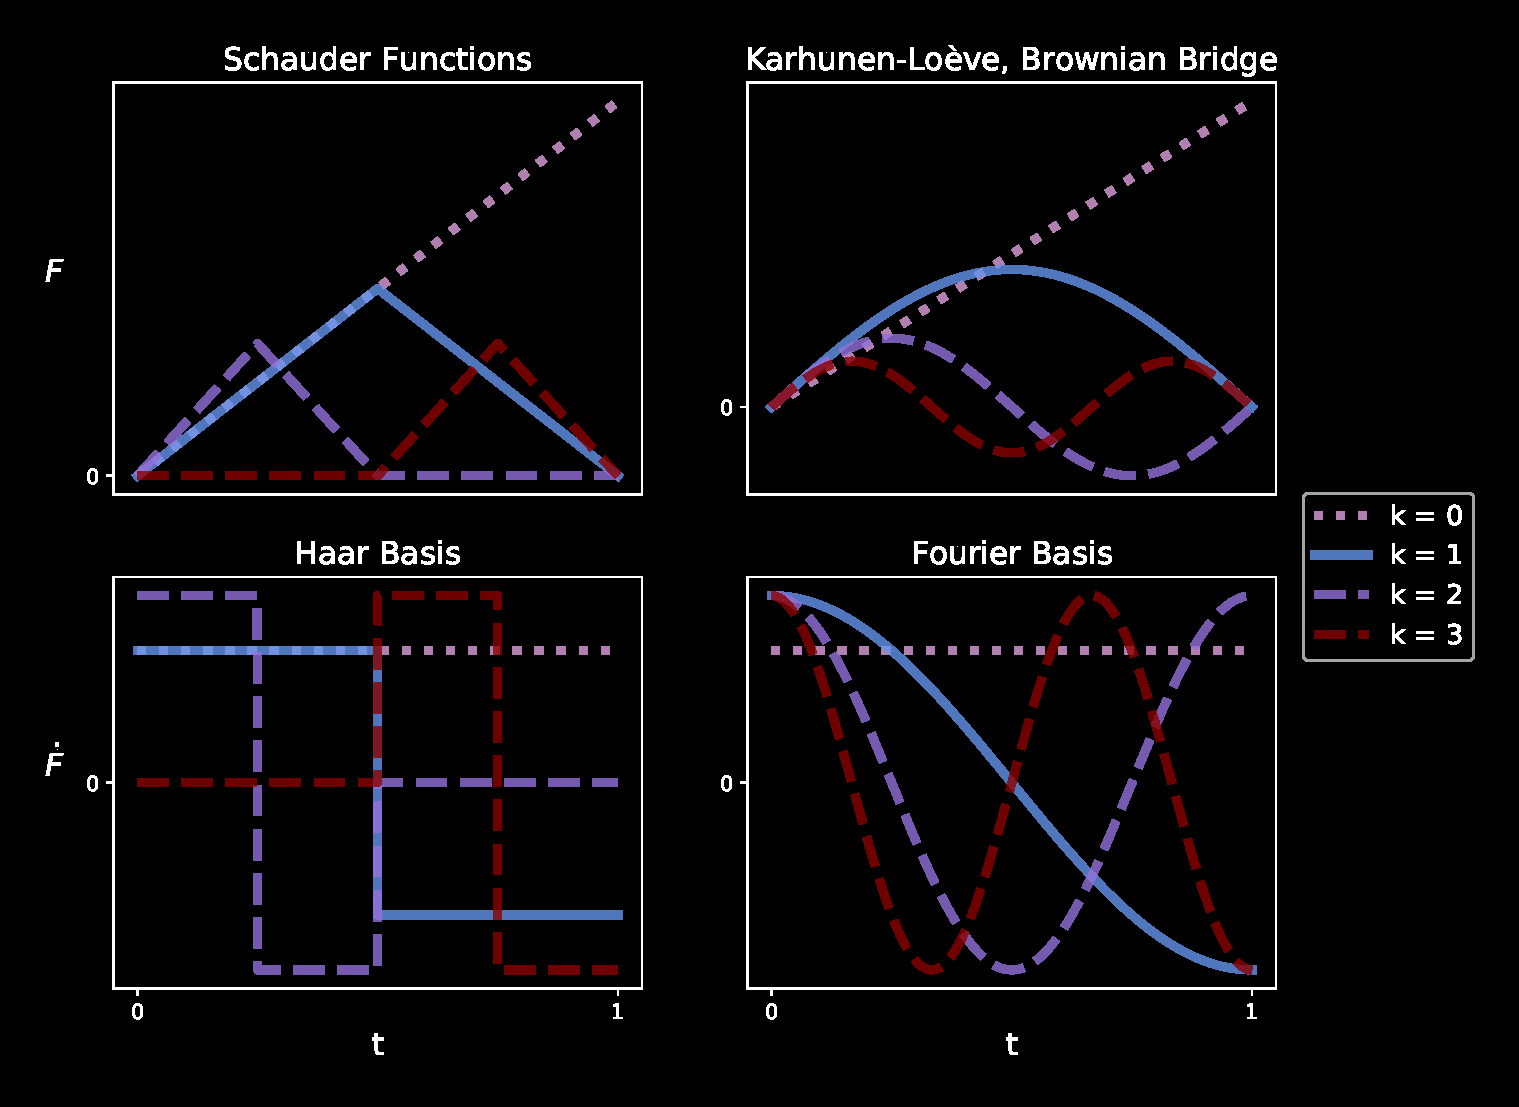
\includegraphics[scale = 0.35]{KL/Figures/LevyCieselski2.pdf}
    \label{fig:CMS}
\end{figure}

\begin{example}\label{ex:BBC}

A standard method to prove the existence of Brownian motion follows from the \text{Brownian bridge construction}. In short, it consists of a random superposition of triangular functions$-$the Schauder functions$-$obtained by integrating the Haar basis on $[0,1]$,
$$\dot{F}_{k,l}(t)=2^{k/2} \, \psi \left(2^{k}t-l\right),\quad 0 \le l \le 2^k,\quad t\in [0,1],$$
with the wavelet $\psi= (-1)^{ \mathds{1}_{[1/2, 1)}}$,  $\textnormal{supp}(\psi) = [0,1]$. It is easily seen that $\dot{F}_{k,l}$ as well as $F_{k,l}$ have support  
$[l/2^k,(l+1)/2^k]$, the $l-$th subinterval of the dyadic partition $\Pi_{k} = \{l/2^k\,|\, l = 0,\ldots,2^k\}$. 
The Schauder and Haar functions are illustrated on the left side of  \Cref{fig:CMS}.  Note that the total number of basis functions employed is $K = |\{(k,l) \,|\, 0 \le l \le 2^k , \, k=0,\ldots, \bar{K} \}| = 2^{\bar{K}+1}-1$ when considering all functions up to the $\bar{K}-$th dyadic partition. 
For Brownian motion, the approximation error is known \cite{Brown} and equal to  $\epsilon^{K,\frakF} = \frac{1}{6K}.$


\end{example}

\begin{example}\label{ex:cosine}
Let $(\dot{F})$ be the \text{cosine Fourier ONB}, i.e.
$\dot{F}_k(t) = \sqrt{2}\cos(\pi k t)$, $t \in [0,1]$. The anti-derivatives $F_k(t) = \sqrt{2}\,\frac{\sin(\pi k t)}{\pi k}$ turns out to correspond$-$up to a factor$-$to the Karhunen-Lo\`eve basis of the \text{Brownian bridge}. Indeed, recalling that $\kappa_X(s,t) = s\wedge t - st$ if $X$ is a Brownian bridge, we have for the ONB $\, \tilde{\frakF} = (\tilde{F}_k) = (\pi k \, F_k)$, 
\begin{align*}
    (\kappa_X(\cdot,t),\tilde{F}_k) 
    = \sqrt{2}\left[(1-t)\int_0^t s\, \sin(\pi k s) ds + t \int_t^1 (1-s)\sin(\pi k s) ds\right]
    = \sqrt{2}\, \frac{\sin(\pi k t)}{\pi^2 k^2},
\end{align*}
using integration by parts in the last equality. 
The eigenvalues  are therefore $(\lambda_k^{\tilde{\frakF}}) = (\frac{1}{\pi^2 k^2})$. 
The first elements of $\tilde{\frakF}$ and the Fourier cosine ONB are displayed on the right charts of  \Cref{fig:CMS}.
Following the same argument as in  \cref{ex:KLBM}, the (minimal) projection error onto $K$ basis functions is approximately equal to $\frac{1}{\pi^2 K}$. This is less than Brownian motion, as little more is known about a Brownian bridge; $\Q-$almost all trajectories return to the origin.

\end{example}

% \begin{figure}[H]
%     \centering
%     \includegraphics[scale = 0.4]{Figures/LevyCieselski.pdf}
%     \caption{Bases in the Cameron-Martin space. }
%     \label{fig:CMS}
% \end{figure}
 
 
 
 
 
 
 
\subsection{Signature and Legendre Polynomials}\label{sec:sigLegendre}
An alternative characterization of a path is available through the so-called \textit{signature}  \cite{Lyons}.  Roughly speaking, the signature extract  from a path an infinite-dimensional skeleton, where  each "bone" contains inherent information. 
We start off with a few definitions. 
A \textit{word} is a sequence  $\alpha = \alpha_1 ... \alpha_k$ of letters from the alphabet $\{0,1\}$. The length of $\alpha$ is denoted  by $l(\alpha)$. 
Moreover, we augment a path $X \in \Lambda$ with the time itself $t \mapsto t$  and   write 
$x^0_{t} = t$, $x^1_{t} = x_t$.  The words $0,1$ are therefore identified with the time $t$ and path $x$, respectively. 
The \textit{signature} in $\Lambda$ is here seen as  a collection  of functionals $\calS= \{\calS_{\alpha}: \Lambda \to \R\}$ such that $\calS_{\emptyset}(X_t) \equiv 1$ and 
$$\calS_{\alpha}(X_t) =
\int_{0}^{t} \int_{0}^{t_k} \cdots \int_{0}^{t_2} \circ \, dx^{\alpha_1}_{t_1} \cdots \circ dx^{\alpha_k}_{t_k}, \qquad l(\alpha)=k \ge 1,$$
     where  $\circ$ indicates Stratonovich integration.\footnote{When either the integrand or  integrator has bounded variation, the integral is in the  Riemann-Stieljes sense  and the symbol $\circ$ can be omitted. \vspace{2mm}} When referring to a specific path $X$, we shall call the sequence $(\calS_{\alpha}(X))$  the \textit{signature of $X$}. If $x_t\in \R^d$ with $d\ge 2$, then the alphabet becomes $\{0,1,\ldots,d\}$ and  the signature is  defined  analogously.  
The first signature functionals read
\begin{align*}
    \calS_{0}(X_t) &= \int_0^t d t_1 = t, &&\calS_{1}(X_t) = \int_0^t \circ \,d x_{t_1} = x_t - x_0,\\
  \calS_{00}(X_t) &= \int_0^t \int_0^{t_2} d t_1 d t_2 =\frac{t^2}{2}, &&\calS_{11}(X_t) = \int_0^t \int_0^{t_2}\circ \, d x_{t_1} \circ d x_{t_2}=\frac{(x_t-x_0)^2}{2},\\
  \calS_{10}(X_t) &= \int_0^t \int_0^{t_2} dx_{t_1}  d t_2 =\int_0^t (x_{s} - x_0) ds, &&\calS_{01}(X_t) = \int_0^t \int_0^{t_2} d t_1 d x_{t_2} =\int_0^t s \,dx_s.
\end{align*}
Keeping track of the passage of time  is crucial, as the signature would otherwise barely carry  information about the path. Indeed, notice that
$\calS_{\alpha}(X_t) = \frac{(x_t-x_0)^{k}}{k!}$ for  $\alpha =  1...1$, $l(\alpha)=k$ 
(as seen above for $k=1,2$) thus only the increment $x_t-x_0$ is known with the alphabet $\{1\}$. 
 
A property of the signature is that it uniquely characterizes a path, up to a  equivalence relation: two paths having same signature differ at most by a \textit{tree-like path} \cite{Hambly}, a specific type of loop.  
Hence, extending a path with time 
not only enriches the  signature  but also
ensures  injectivity  as $t\to x^0_t =t$ is increasing. 
This gives hope to reconstruct the (unique) path associated to a  signature sequence. This was investigated 
 by \citet{Geng}, where the author shows a 
geometric reconstruction using polygonal approximations for Brownian paths. 
We propose a simple algorithm, in connection with our discussion on Hilbert projections.\footnote{I thank Bruno Dupire for suggesting this interesting parallel.} 
For ease of presentation, assume $x_0=0$ and $T=1$. We first make the following observation. 

\begin{lemma}\label{lem:Legendre}
Let $\overleftarrow{X}$ denote the \textit{time reversed path}, i.e. $\overleftarrow{\ x_t} = x_{1-t}$ and 
introduce the words $\alpha^{(k)} :=10\ldots0\,$, $l(\alpha^{(k)})=k+2$, $k \ge 0$. 
Then $\calS_{\alpha^{(k)}} (\overleftarrow{X}_{\! 1})  = \frac{1}{k!}(X, m_k) $ where $m_k(t)=t^k$.
\end{lemma}
\begin{proof} First, observe that 
\begin{equation}\label{eq:100}
    \calS_{\alpha^{(k)}}(X_{t}) = \int_0^{t} x_s \frac{(t -s)^{k}}{k!}ds,\quad \forall \, t \in [0,1]. 
\end{equation}
Indeed for fixed $t\in [0,1]$ and  $k=0$, then $\calS_{\alpha^{(0)}}(X_t)=\calS_{10}(X_t) = \int_0^t x_sds$, which is $\eqref{eq:100}$. Now by induction on $k\ge 1$, uniformly on $[0,t]$,
\begin{align*}
  \calS_{\alpha^{(k)}}(X_t) = \int_0^t \calS_{\alpha^{(k-1)}}(X_u)du 
    = \int_0^t \int_0^u x_s \frac{(u -s)^{k-1}}{(k-1)!}ds\, du 
    = \int_0^t x_s \frac{(t -s)^{k}}{k!} ds.
\end{align*}
Now taking $t=1$ and $\overleftarrow{X}$ instead of $X$, we get
$
    \calS_{\alpha^{(k)}}(\overleftarrow{X}_{\! 1}) = \int_0^1 \overleftarrow{\ x_t}\frac{(1 -t)^{k}}{k!}dt =  \frac{1}{k!}(x,m_k).
$
\end{proof}

Essentially,  \Cref{lem:Legendre} states that the knowledge of $(\calS_{\alpha^{(k)}}(\overleftarrow{X}_{\! 1}))_{k\ge 0}$ is equivalent to the knowledge of the inner products of the path with the monomials. Since  also 
\begin{align*}
    \calS_{\alpha^{(k)}}(\overleftarrow{X}_{\! 1})
    &= (-1)^{k}\int_0^1 x_t \frac{((1-t)-1)^{k}}{k!}dt 
    %= (-1)^{k} \sum_{j=0}^k {k \choose j} \int_0^1 x_t \frac{(1-t)^{j}(-1)^{k-j}}{k!}dt \\
    = \sum_{j=0}^{k} \calS_{\alpha^{(j)}}(X_1) \frac{(-1)^{j}}{(k-j)!},
\end{align*}
the coefficients $(X,m_k)_{k\ge 0}$ can be retrieved from $(\calS_{\alpha^{(k)}}(X_1))_{k\ge 0}$ as well. 
To fall within the context of orthonormal projection, we transform the monomials into the (unique) polynomial ONB of $L^2([0,1])$. 
Let $(p_k)$ be the Legendre polynomials \cite{Szego}, forming an orthogonal basis of $L^2([-1,1])$. Then  consider the \textit{shifted Legendre polynomials},  $q_k(t) = p_k(2t-1),$  $t\in [0,1].$ 
We write 
$$q_k(t)= \sum_{j\le k} a_{k,j}t^j, \quad a_{k,j} = (-1)^{k+j} {k \choose j} {k + j \choose j},$$ with coefficients  derived for instance from  \textit{Rodrigues' formula} \cite[Section 4.3]{Szego}. The standardization $F_k :=  \frac{q_k}{\lVert q_k\rVert} = \sqrt{2k+1}q_k$ makes $\frakF = (F_k)$ an ONB of $L^2([0,1])$. This leads us to the following result. 
\begin{proposition}
If  $b_{k,j} := \sqrt{2k+1} j!\, a_{k,j}$ and $G_j(t) := \sum_{k= j}^K b_{k,j}\,  F_k(t)$, then 
\begin{equation}\label{eq:sigLeg}
    x^{K,\frakF}_t 
    = \sum_{k\le K} \xi_k F_k(t)
    =  \sum_{j \le K} \calS_{\alpha^{(j)}}(\overleftarrow{X_1})  G_j(t).
\end{equation}
\end{proposition}

\begin{proof}
 First, note that $(X,F_k) = \sum_{j\le k} a_{k,j}\, (X,m_j)$.   Using \cref{lem:Legendre}, we obtain 
$\xi_k = \sum_{j \le k} b_{k,j}\, \calS_{\alpha^{(j)}}(\overleftarrow{X_1})$. Hence,   $ x^{K,\frakF}_t   = \sum_{j \le K} \calS_{\alpha^{(j)}}(\overleftarrow{X_1})  G_j(t)$ with $(G_j)$ as in the statement.
\end{proof}
In summary, the signature elements $(\calS_{\alpha^{(k)}})_{k\le K}$ generate the $L^2([0,1])$ products of the path with the monomials$-$and in turn, with the Legendre polynomials$-$from which the projected path $X^{K,\frakF} $ becomes available. 
We can therefore retrieve $X$ by letting $K\to \infty$. Note that this reconstruction  works for multidimensional paths as well, as we can apply the procedure to each component  $i=1,\ldots,d$ with the words
$\alpha^{(i,k)} :=i 0\ldots0$, $l(\alpha^{(i,k)}) = k+2$, $k \ge 0$.  
We finish this section by computing the projection error of $\eqref{eq:sigLeg}$ when $X$ is Brownian motion. Recalling that $\kappa_X(s,t) = s \wedge t$,  a  simple calculation gives 
$$\lambda_k^{\frakF} = \E^{\Q}[\xi_k^2] = 2 \int_{0}^1 \int_{0}^t s  F_k(s)dsF_k(t)dt = 2 (2k+1)\sum_{i,j \le k} \frac{a_{k,j}\ a_{k,i}}{(j+2)(i+j+3)}.
%(-1)^{k+j} {k \choose j} {k + j \choose j}
$$
 
The first values are given by $(\lambda^{\frakF}_k)_{k=0}^3 = (\frac{1}{3},\frac{1}{10}, \frac{1}{42}, \frac{1}{90})$ from which we  conjecture that $\lambda^{\frakF}_k = \frac{1}{(2k+3)(4k-2)}$ for all $k\ge 1$. This is supported by the fact that $\lambda^{\frakF}_k$ must be  rational numbers as $a_{k,j}\in \Z$ for all $k,j$ and 
$$\sum_{k=0}^K  \lambda^{\frakF}_k = \frac{1}{3} + \frac{1}{8} \sum_{k=1}^K  \left( \frac{1}{2k-1}-\frac{1}{2k+3} \right) = \frac{1}{2} - \frac{K+1}{(2K+3)(4K+2)} \xrightarrow{K \uparrow \infty} \frac{1}{2},$$ coinciding with the total variance of Brownian motion on $[0,1]$.  
Thus, the approximation error reads  $\epsilon^{K, \frakF} =\frac{K+1}{(2K+3)(4K+2)} = \calO(\frac{1}{8K})$, which is of course larger than the Karhunen-Loève basis but smaller than the Brownian Bridge construction (\cref{ex:BBC}). Note that polynomial ONB's may well be optimal if the approximation criterion is modified. In \cite{Foster}, the authors show that in the weighted Hilbert space $L^2([0,1],\mu)$, $\mu(dt) = \frac{dt}{t(1-t)}$, the Karhunen-Loève basis of the Brownian bridge is formed by the anti-derivatives of the Legendre polynomials. Although the construction is different, it  is also curiously related to the signature elements $(\calS_{\alpha^{(k)}})$; see  Theorem 2.3 and  2.4 in \cite{Foster}.

%In \cite{Foster}, the authors show that representation of Brownian motion with polynomials arising from the Karhunen-Loève expansion of the Brownian bridge in the weighted Hilbert space $L^2([0,1],\mu)$, $\mu(dt) = \frac{dt}{t(1-t)}$ is .  Therefore, a polynomial ONB may well be optimal if the approximation criterion is modified. Although the polynomial expansion is different, the same signature elements appear;  in \cite{Foster}; .

\begin{remark}
Note that the approximation in $\eqref{eq:sigLeg}$ may be improved by adding other elements of the  signature, especially those that are \textit{nonlinear} in $X$, e.g. $\calS_{110}(X_t) = \frac{1}{2}\int_0^t x^2_s ds $.  We postpone this discussion to  \Cref{sec:sigFunc} when projecting  running functionals.
\end{remark} 
 
 \begin{figure}[t]
    \centering
    \caption{Projected paths with $K=8\,$ basis elements. }
    \vspace{-2mm}
    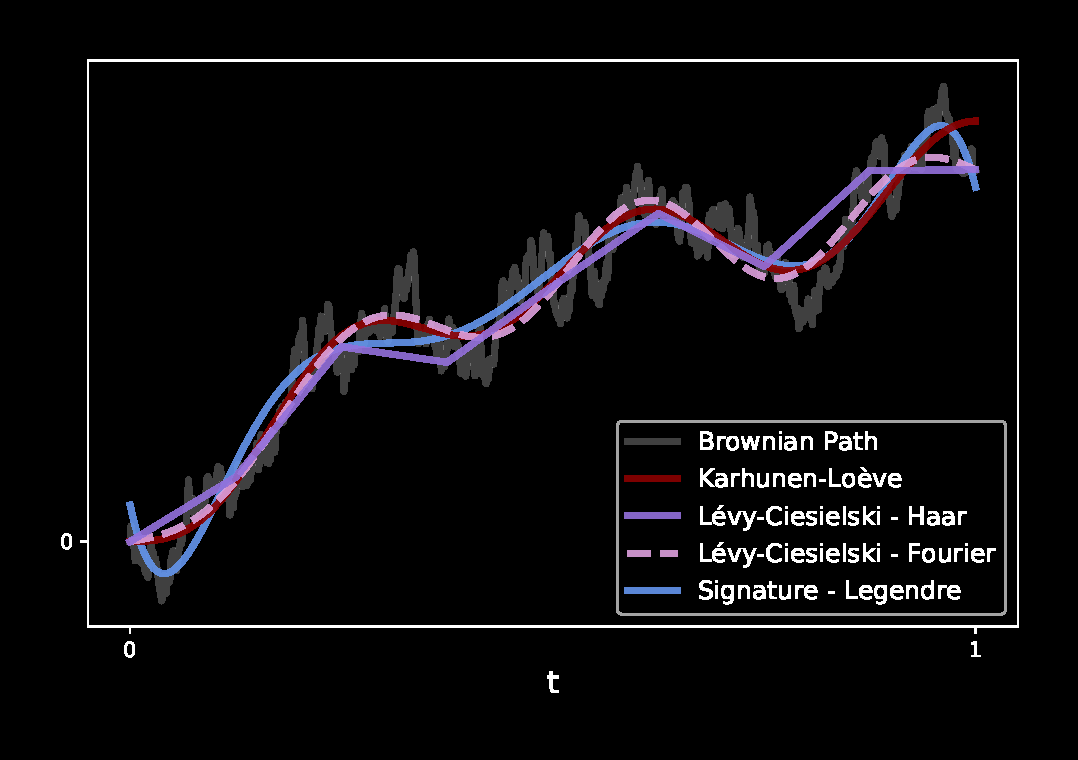
\includegraphics[scale = 0.45
    ]{KL/Figures/ProjPath.pdf}
    \label{fig:projPath}
\end{figure}
 \subsection{Numerical Results}\label{sec:numResultX}

We concentrate our experiments on Brownian trajectories.  
First, we illustrate %visualize and compare 
the  path  approximations seen earlier (Karhuhen-Loève, L\'evy-Cieselski, Signature).
Figure \ref{fig:projPath} displays the projections using $K=8$ basis elements. We naturally notice similarities between the Karhunen-Loève transform and the L\'evy-Cieselski construction with Fourier cosines, both 
obtained by superposing trigonometric functions.

Let us gauge the accuracy of the above approximations for Brownian trajectories, in terms of (i) 
    $\epsilon^{K,\frakF}$ and (ii) variance explained 
    $ \vartheta^{K,\frakF} := \frac{\lVert X^{K,\frakF}  \rVert^2_{*}}{\left \lVert X \right \rVert^2_{*}}.$ 
To compute (i), (ii) and the coefficients $(X,F_k)_{\calH}$, we discretize the interval $[0,1]$ a regular partition made of $N = 10^4$ subintervals. 
\Cref{fig:Error_VarExp} displays the evolution of $\epsilon^{K,\frakF}$, $\vartheta^{K,\frakF}$ for $K\in \{1,\ldots,128\}$. The Karhunen-Lo\`eve expansion clearly dominates the other projections, although being asymptotically equivalent to the L\'evy-Cieselski construction with Fourier cosine basis. Besides, the $L^2(\mathbb{Q} \, \otimes \, dt)$ convergence of the Brownian bridge construction (L\'evy-Cieselski with Haar basis) is non-monotonic. Indeed, a bump appears until a full cycle of the dyadic partition is completed. 
Lastly, the slopes in the log-log convergence plot  (left chart of \Cref{fig:Error_VarExp}) 
are roughly equal to $-1$. Put differently,  the squared approximation error is of order $\calO(\frac{1}{K})$, confirming our findings from the  above examples.

\begin{figure}[t]
    \centering
    \caption{$L^2(\mathbb{Q} \, \otimes \, dt)$ error and variance explained.}
    \vspace{-2mm}
    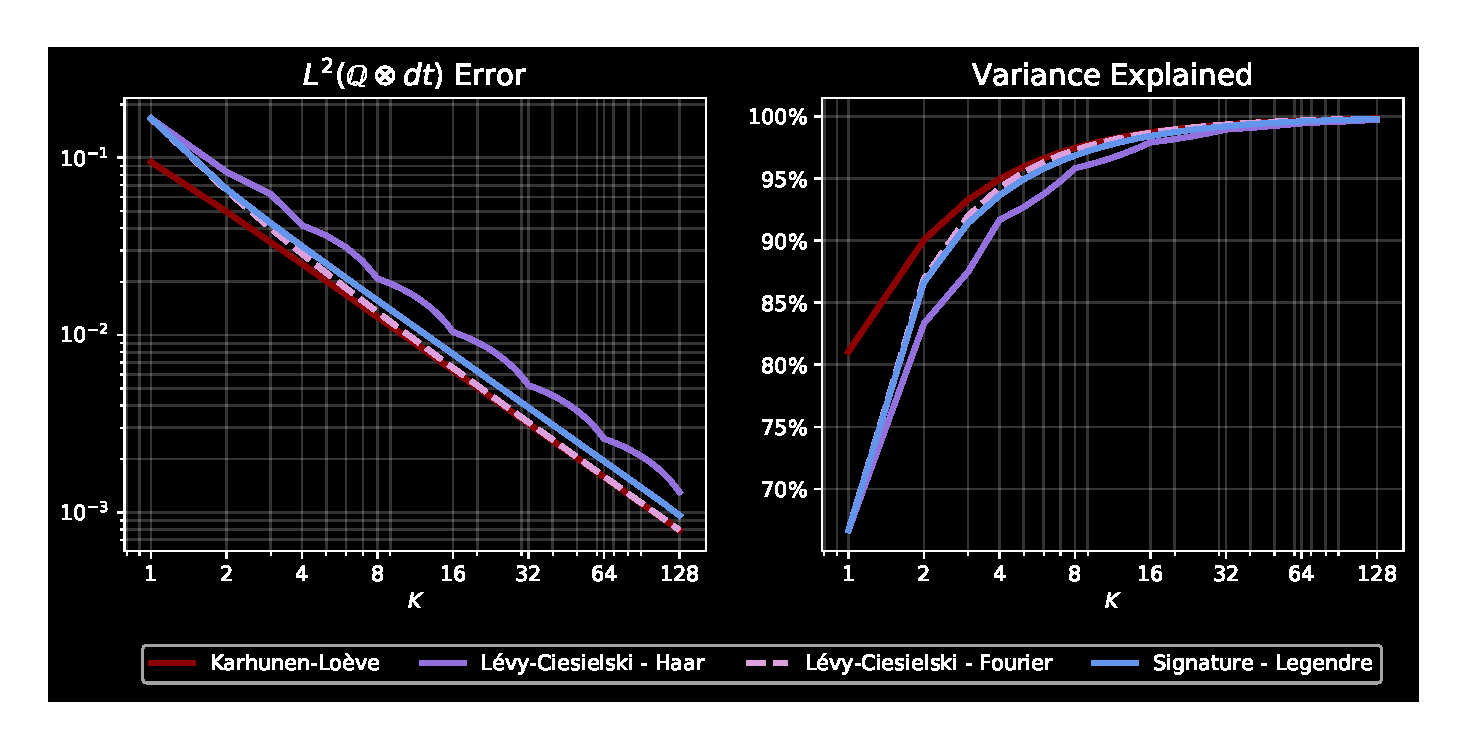
\includegraphics[scale = 0.45]{KL/Figures/Err_VarExp.pdf}
    \label{fig:Error_VarExp}
\end{figure}
 
\section{Projection of Functionals}
\label{sec:funcApprox}
In  \Cref{sec:pathApprox}, we unveiled two ways to approximate exotic payoffs $\varphi = h\circ f$, namely by projecting the original path $X$ or $Y = f(X)$ directly.  If $\pi^{K,\frakF}$ denotes as before the projection map onto a Hilbert space $\calH$, we can therefore write $\varphi^{K,\frakF} := h\circ f^{K,\frakF}$, where either $f^{K,\frakF} = f \circ \pi^{K,\frakF}$ (functional of projected path)
or $f^{K,\frakF} = \pi^{K,\frakF} \circ f$ (projected functional). 
% This implies that the transformed path is projected  we can either take the image of the projected path  $(Y^{K,\frakF} = (\pi^{K,\frakF} \circ f)(X))$ or project $f(X)$ directly  $(Y^{K,\frakF} = (\pi^{K,\frakF} \circ f)(X))$. 
% This consists of taking the image of a projected path through the functional, namely $Y^{K,\frakF} =  f(X^{K,\frakF})$. 
We shall see in  \Cref{ssec: numResult} that the former is suboptimal. 
Although not so problematic for functionals capturing global features of a path, local path characteristics (e.g. running maximum) will typically be grossly estimated. Indeed, projecting a path first erases most of its microstructure. 
We thus favor the second option ($f^{K,\frakF} = \pi^{K,\frakF} \circ f$), which consists of replacing $X$ by $Y$ in $\eqref{eq:proj}$. Let us now focus on $\calH = L^2([0,T])$ and demonstrate how to compute the Karhunen-Loève basis of $Y$. 



\subsection{Karhunen-Loève Expansion of Functionals}



Assume that $Y \in L^2([0,T]) \cap \Lambda_T$ has  zero mean (otherwise, see \cref{rem:center}).   \cref{thm:KL} suggests to set  $\frakF$  equal to the eigenfunctions of  $\kappa_Y(s,t) = (y_s,y_t)_{L^2(\Q)}$. Optimality comes, however,  at the cost of explicitizing $\frakF$. We proceed as follows: take a regular partition $\Pi_N = \{t_n = n\, \delta t\, |\, n=0,\ldots,N\}$, $ \delta t =\frac{T}{N}$ and compute the kernel matrix $\kappa^{N}_Y = (\kappa_Y(t_n,t_m))_{0 \le n,m \le N}$. When $\kappa_Y$ does not admit a  closed-form expression, $\kappa^{N}_Y$ is replaced by the sample covariance matrix using simulated paths for $Y$. The eigenfunctions thus become eigenvectors and solve the systems\footnote{In  $\eqref{eq:eigendecomp}$,  $\sum"$ means that the first and last summand are halved, i.e. the trapezoidal rule is used to compute  $(\kappa_Y(\cdot,t), F_k)$. Another approach, known as Nyström's method  \cite{reinhardt} consists of   employing a Gaussian quadrature scheme instead.  
However, for large $N$,  we haven't observed any improvement 
and thus favor the more convenient discretization in  $\eqref{eq:eigendecomp}$.}
\vspace{-1mm}
\begin{equation}\label{eq:eigendecomp}
        \sum_{t_n\in  \Pi_N}\!\!" \, \kappa^{N}_{Y}(t_n,t_m) F_{k}(t_n)  \delta t = \lambda^{\frakF}_{k}\,  F_{k}(t_m), \quad t_m\in \Pi_N, \quad k=0,...,N.
\end{equation}
\vspace{-3mm}

 This is a simple eigenvalue problem so  all pairs $(F_k,\lambda_k^{\frakF})$ can be  computed in one go. Let us proceed with two examples where  $T=1$ and $\Q=$ Wiener measure throughout.

\begin{figure}[t]
    \centering
    \caption{Running maximum functional for two trajectories.}
    \vspace{-2mm}
    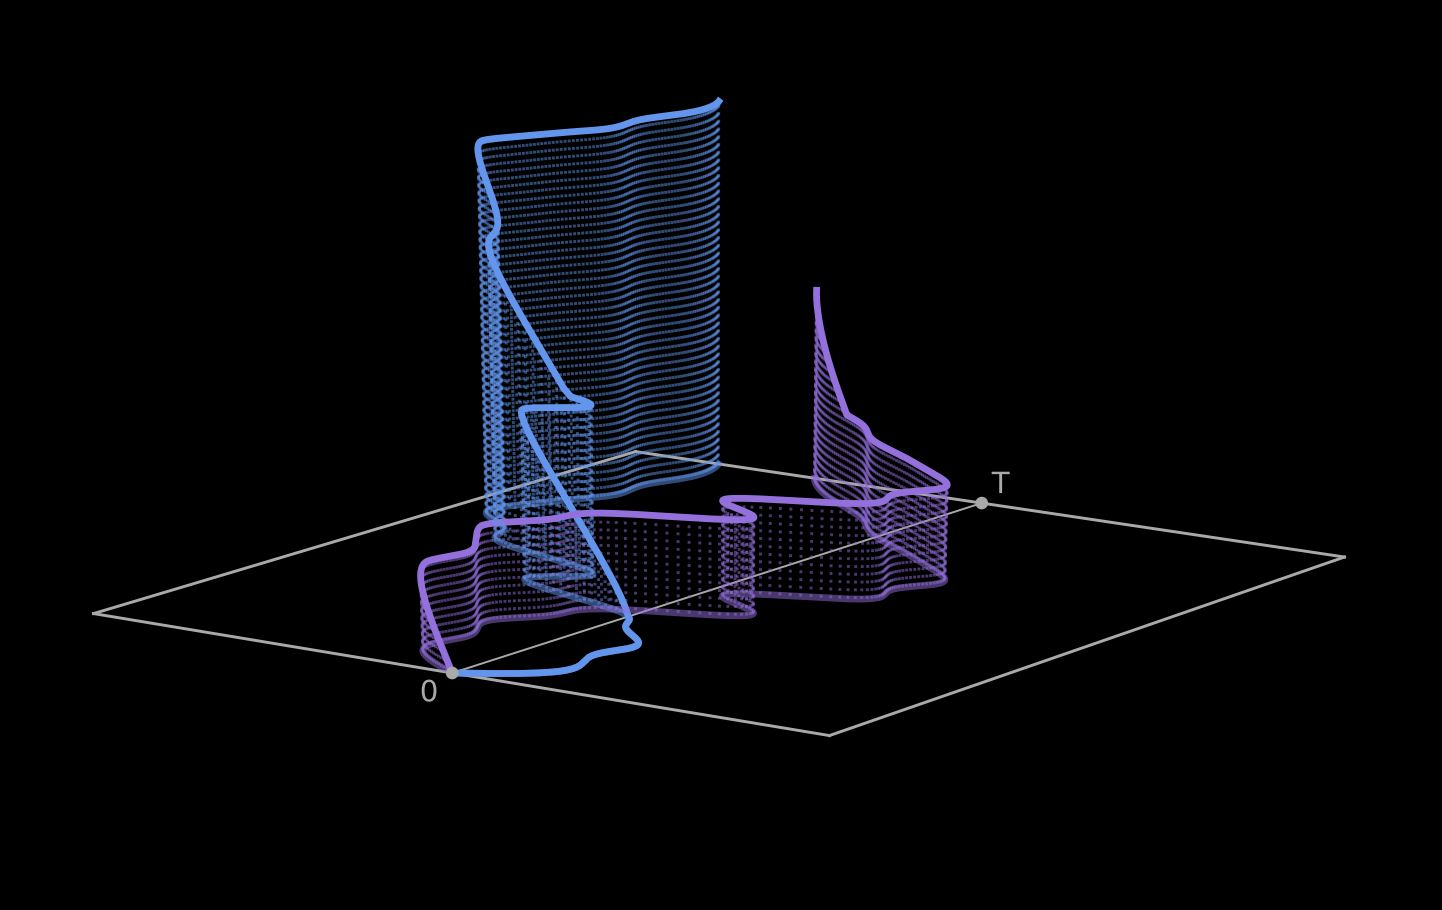
\includegraphics[scale =0.22]{KL/Figures/MaxDouble.JPG}
    %
    \label{fig:max3D}
\end{figure}



%========== Time Average and Integral ===========%
\begin{example} \label{ex:timeIntAvg}
 Consider  the time integral and average of a Brownian path, 
$y_t = 
f(X_t) = \int_0^t x_s\, ds, \ \bar{y}_{t}= 
\bar{f}(X_t) = \frac{1}{t}f(X_t). $
These are clearly centered processes and their covariance kernels of can be found explicitly. Starting with $Y$, 
$$\kappa_{Y}(s,t) =  \left(\int_0^s x_r dr,\int_0^t x_u du \right)_{L^2(\Q)} \overset{\textnormal{Fubini}}{=} \int_0^s\int_0^t \kappa_X(r,u) dr du.$$
A straightforward calculation gives
$\kappa_{Y}(s,t)  = \frac{s^2 t}{2} - \frac{s^3}{6}, \, s\le t.$
%\textbf{Moreover, it is straightforward to show that the eigenvalues are the square of the eigenvalues of Brownian (see Example \ref{ex:KLBM}).}
The covariance function of the time average follows immediately, namely
$\kappa_{\bar{Y}}(s,t)   = \frac{s}{2} -\frac{s^2}{6t}.$
We display in  \Cref{fig:AvgK,fig:IntK} the covariance kernel (top) and first eigenfunctions (bottom) of $f$ and $\bar{f}$, respectively.
The dashed lines in the top panels  are the eigenfunctions of the original (Brownian) path. Note the wider range in the eigenfunctions $F_1,F_2$ for $\bar{f}(X)$ compared to the integrated path for small $t$.  This might come from the greater fluctuations of the time average at inception. 

\end{example}
%========== Maximum ===========%
\begin{example} Consider the running maximum  functional $y_t= 
f(X_t) = \max_{0 \le s \le t} x_s$.  \Cref{fig:max3D} provides an illustration in the $(t,X,Y)$ plane. The mean function is in this case non-zero and$-$using, e.g., the reflection principle$-$given by $\E^{\Q}[y_t] = \sqrt{\frac{2}{\pi} t}$. The covariance kernel admits an explicit yet complicated expression \cite{Benichou}, 
$$\kappa_Y(s,t) = \frac{s}{2} + \frac{\sqrt{s(t-s)}-2\sqrt{st} + t \arcsin(\sqrt{s/t})}{\pi}, \quad s \le t.$$
\Cref{fig:MaxK} displays the covariance kernel (top) and first eigenfunctions (bottom). The latter turns out to be quite close to the eigenfunctions of Brownian motion. 

\end{example}



\begin{figure}[t]%[H]
%\centering
\caption{Covariance kernels (top) and eigenfunctions (bottom).}
\vspace{-4mm}
\begin{subfigure}[b]{0.32\textwidth}
    \centering
    \caption{Time average}
    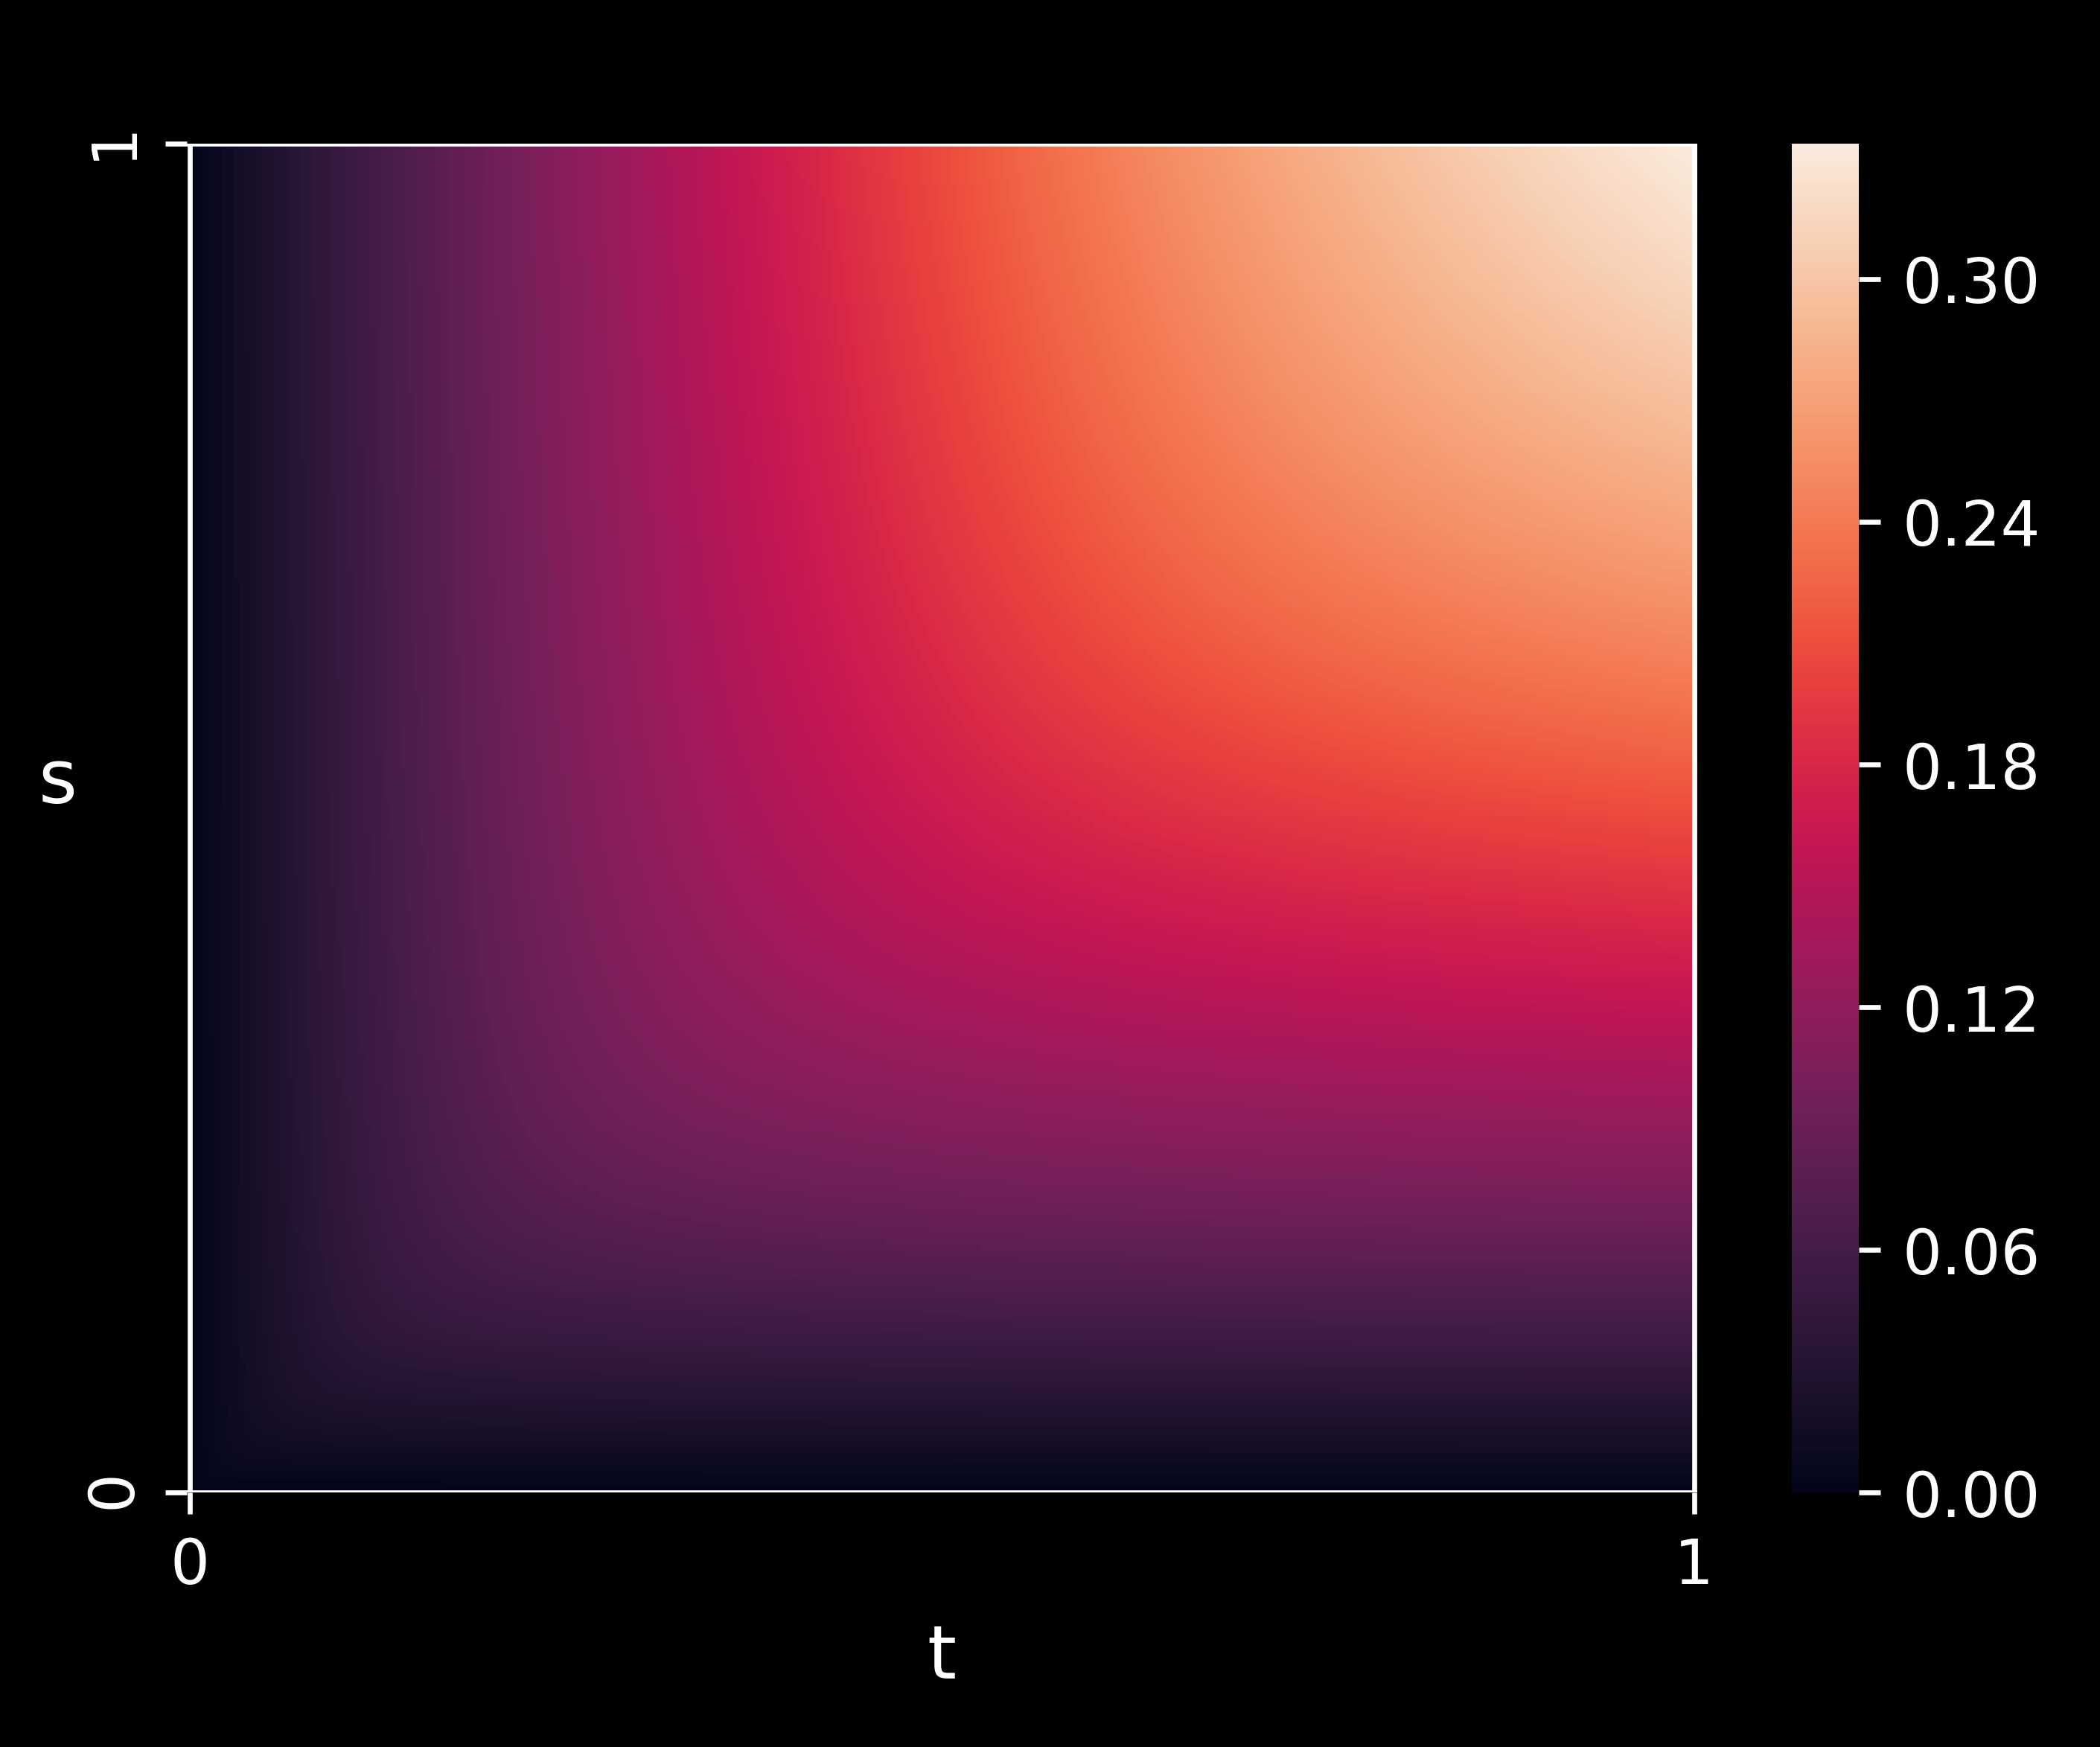
\includegraphics[scale =0.38]{KL/Figures/KLAverageKernel.png}
    \label{fig:AvgK}
\end{subfigure}
\begin{subfigure}[b]{0.32\textwidth}
    \centering
    \caption{Time integral}
    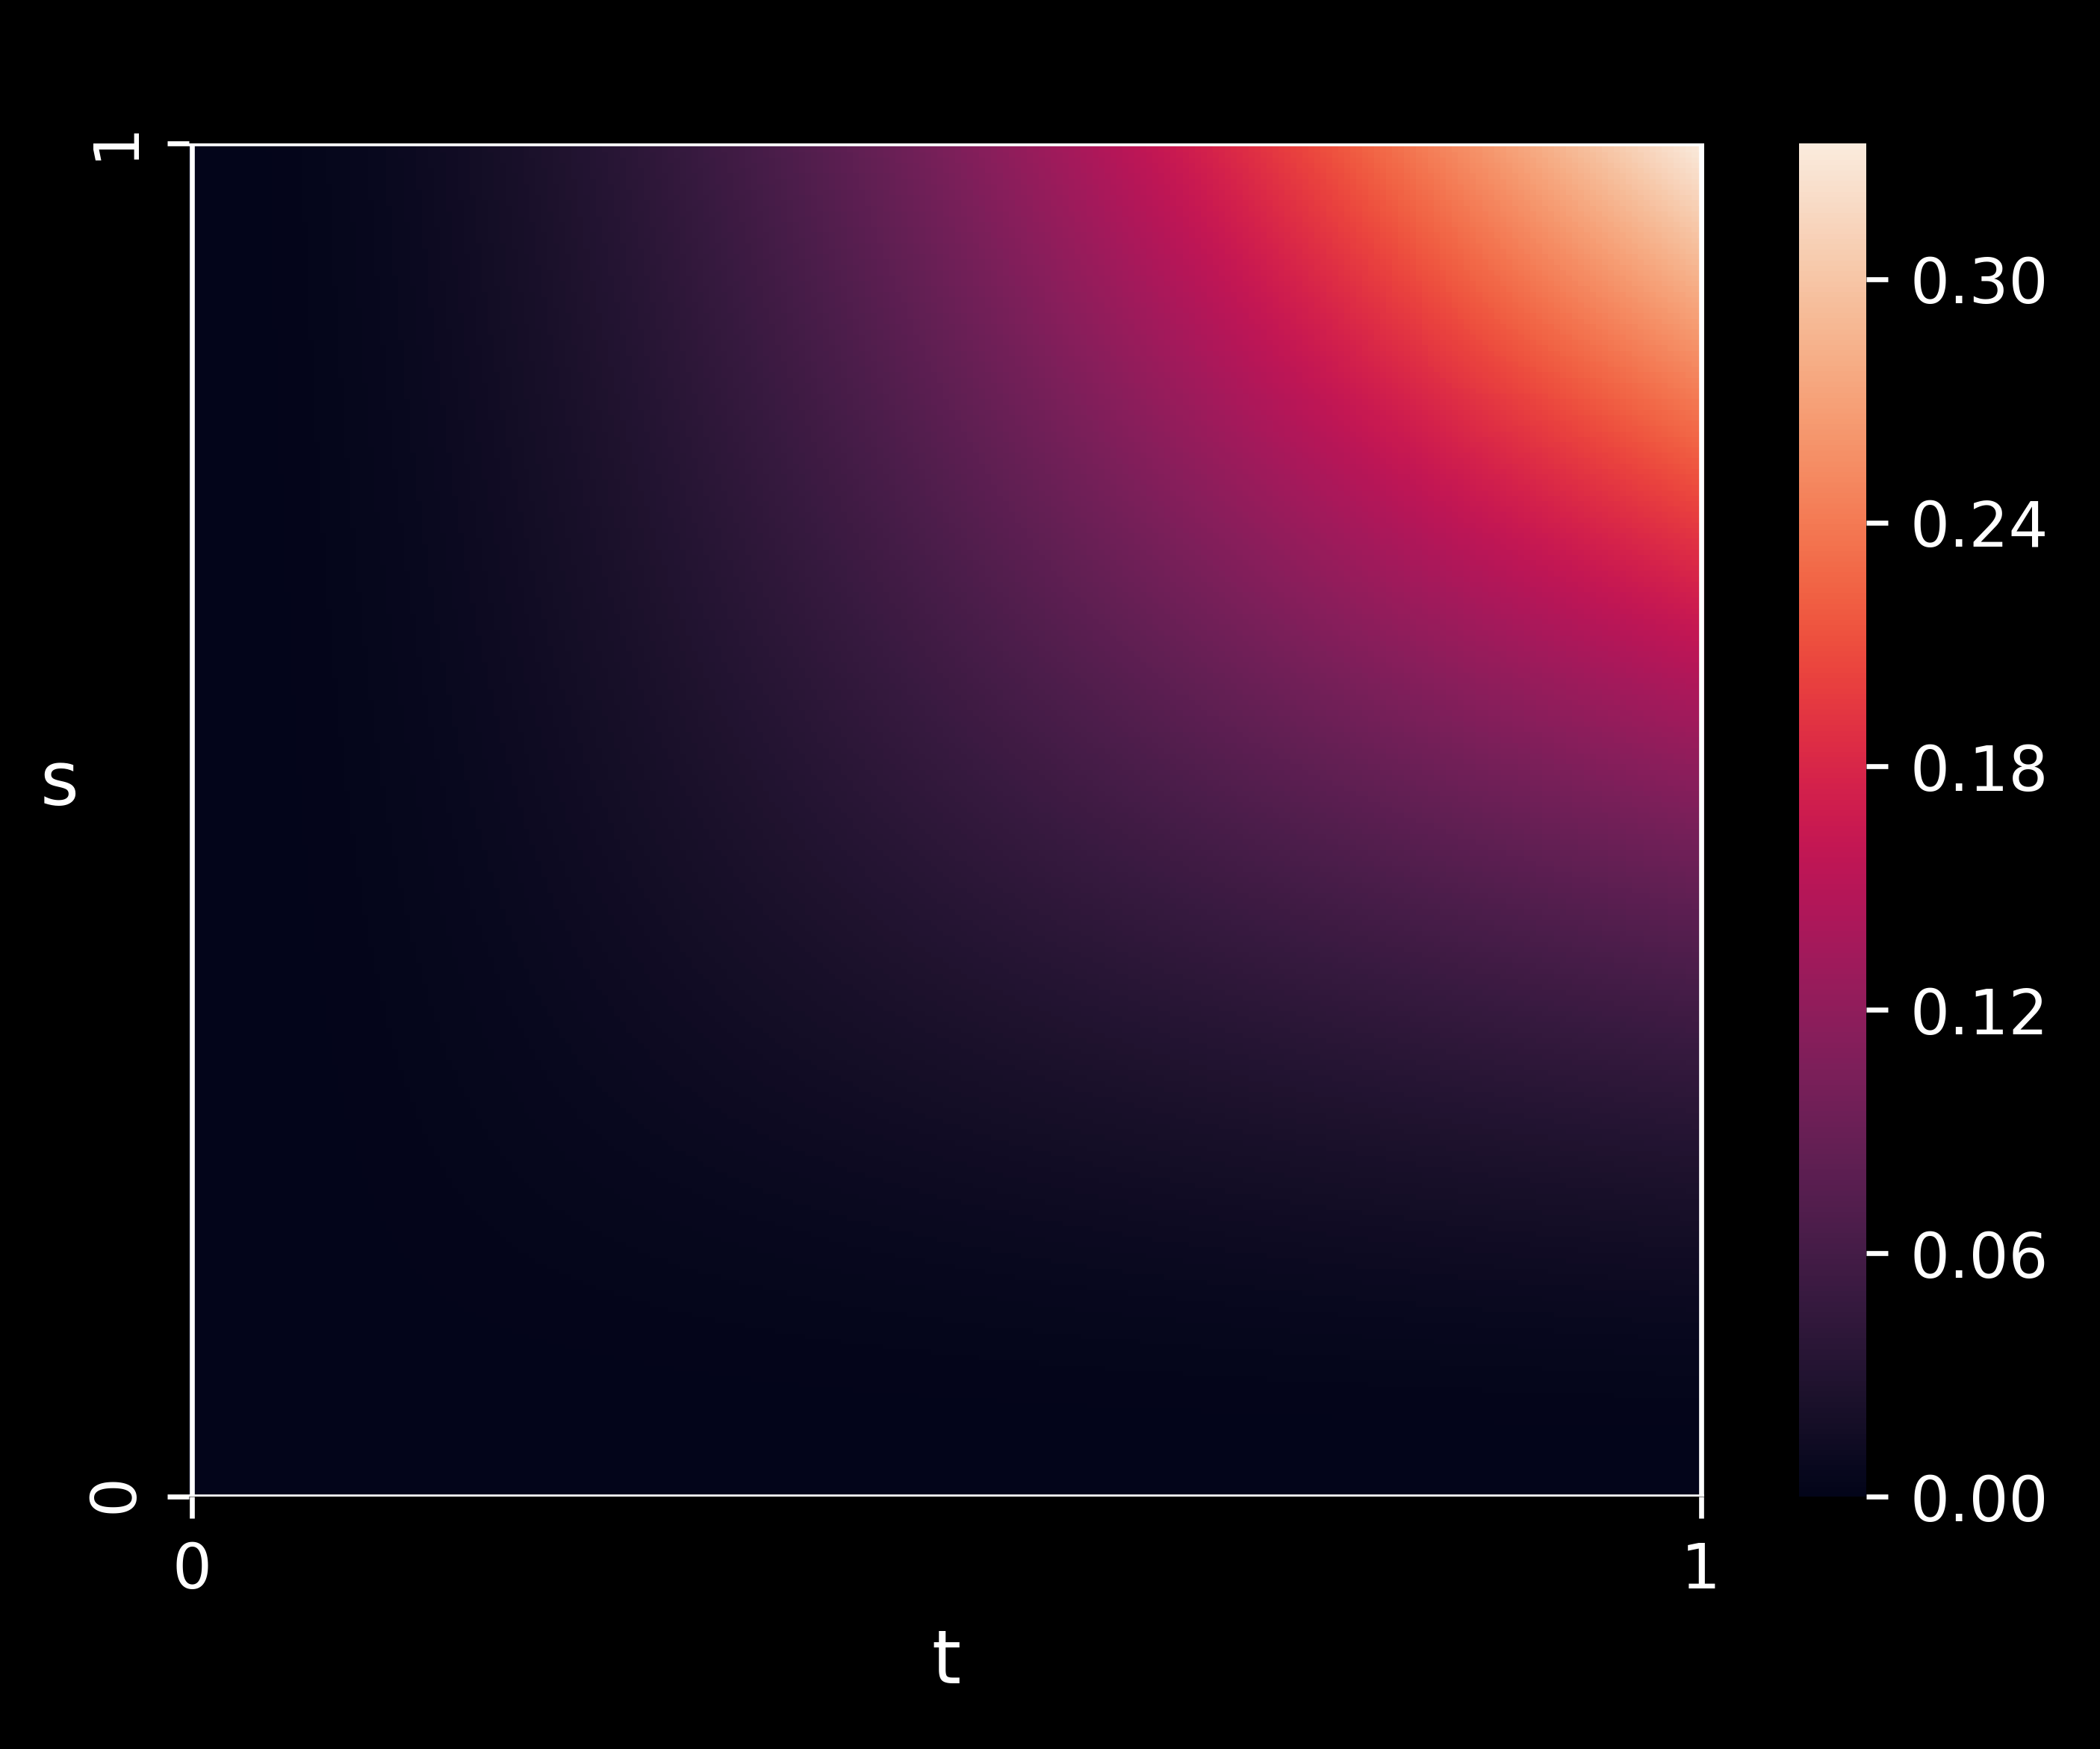
\includegraphics[scale =0.38]{KL/Figures/KLIntegralKernel.png}
    \label{fig:IntK}
\end{subfigure}
\begin{subfigure}[b]{0.32\textwidth}
    \centering
    \caption{Running maximum}
    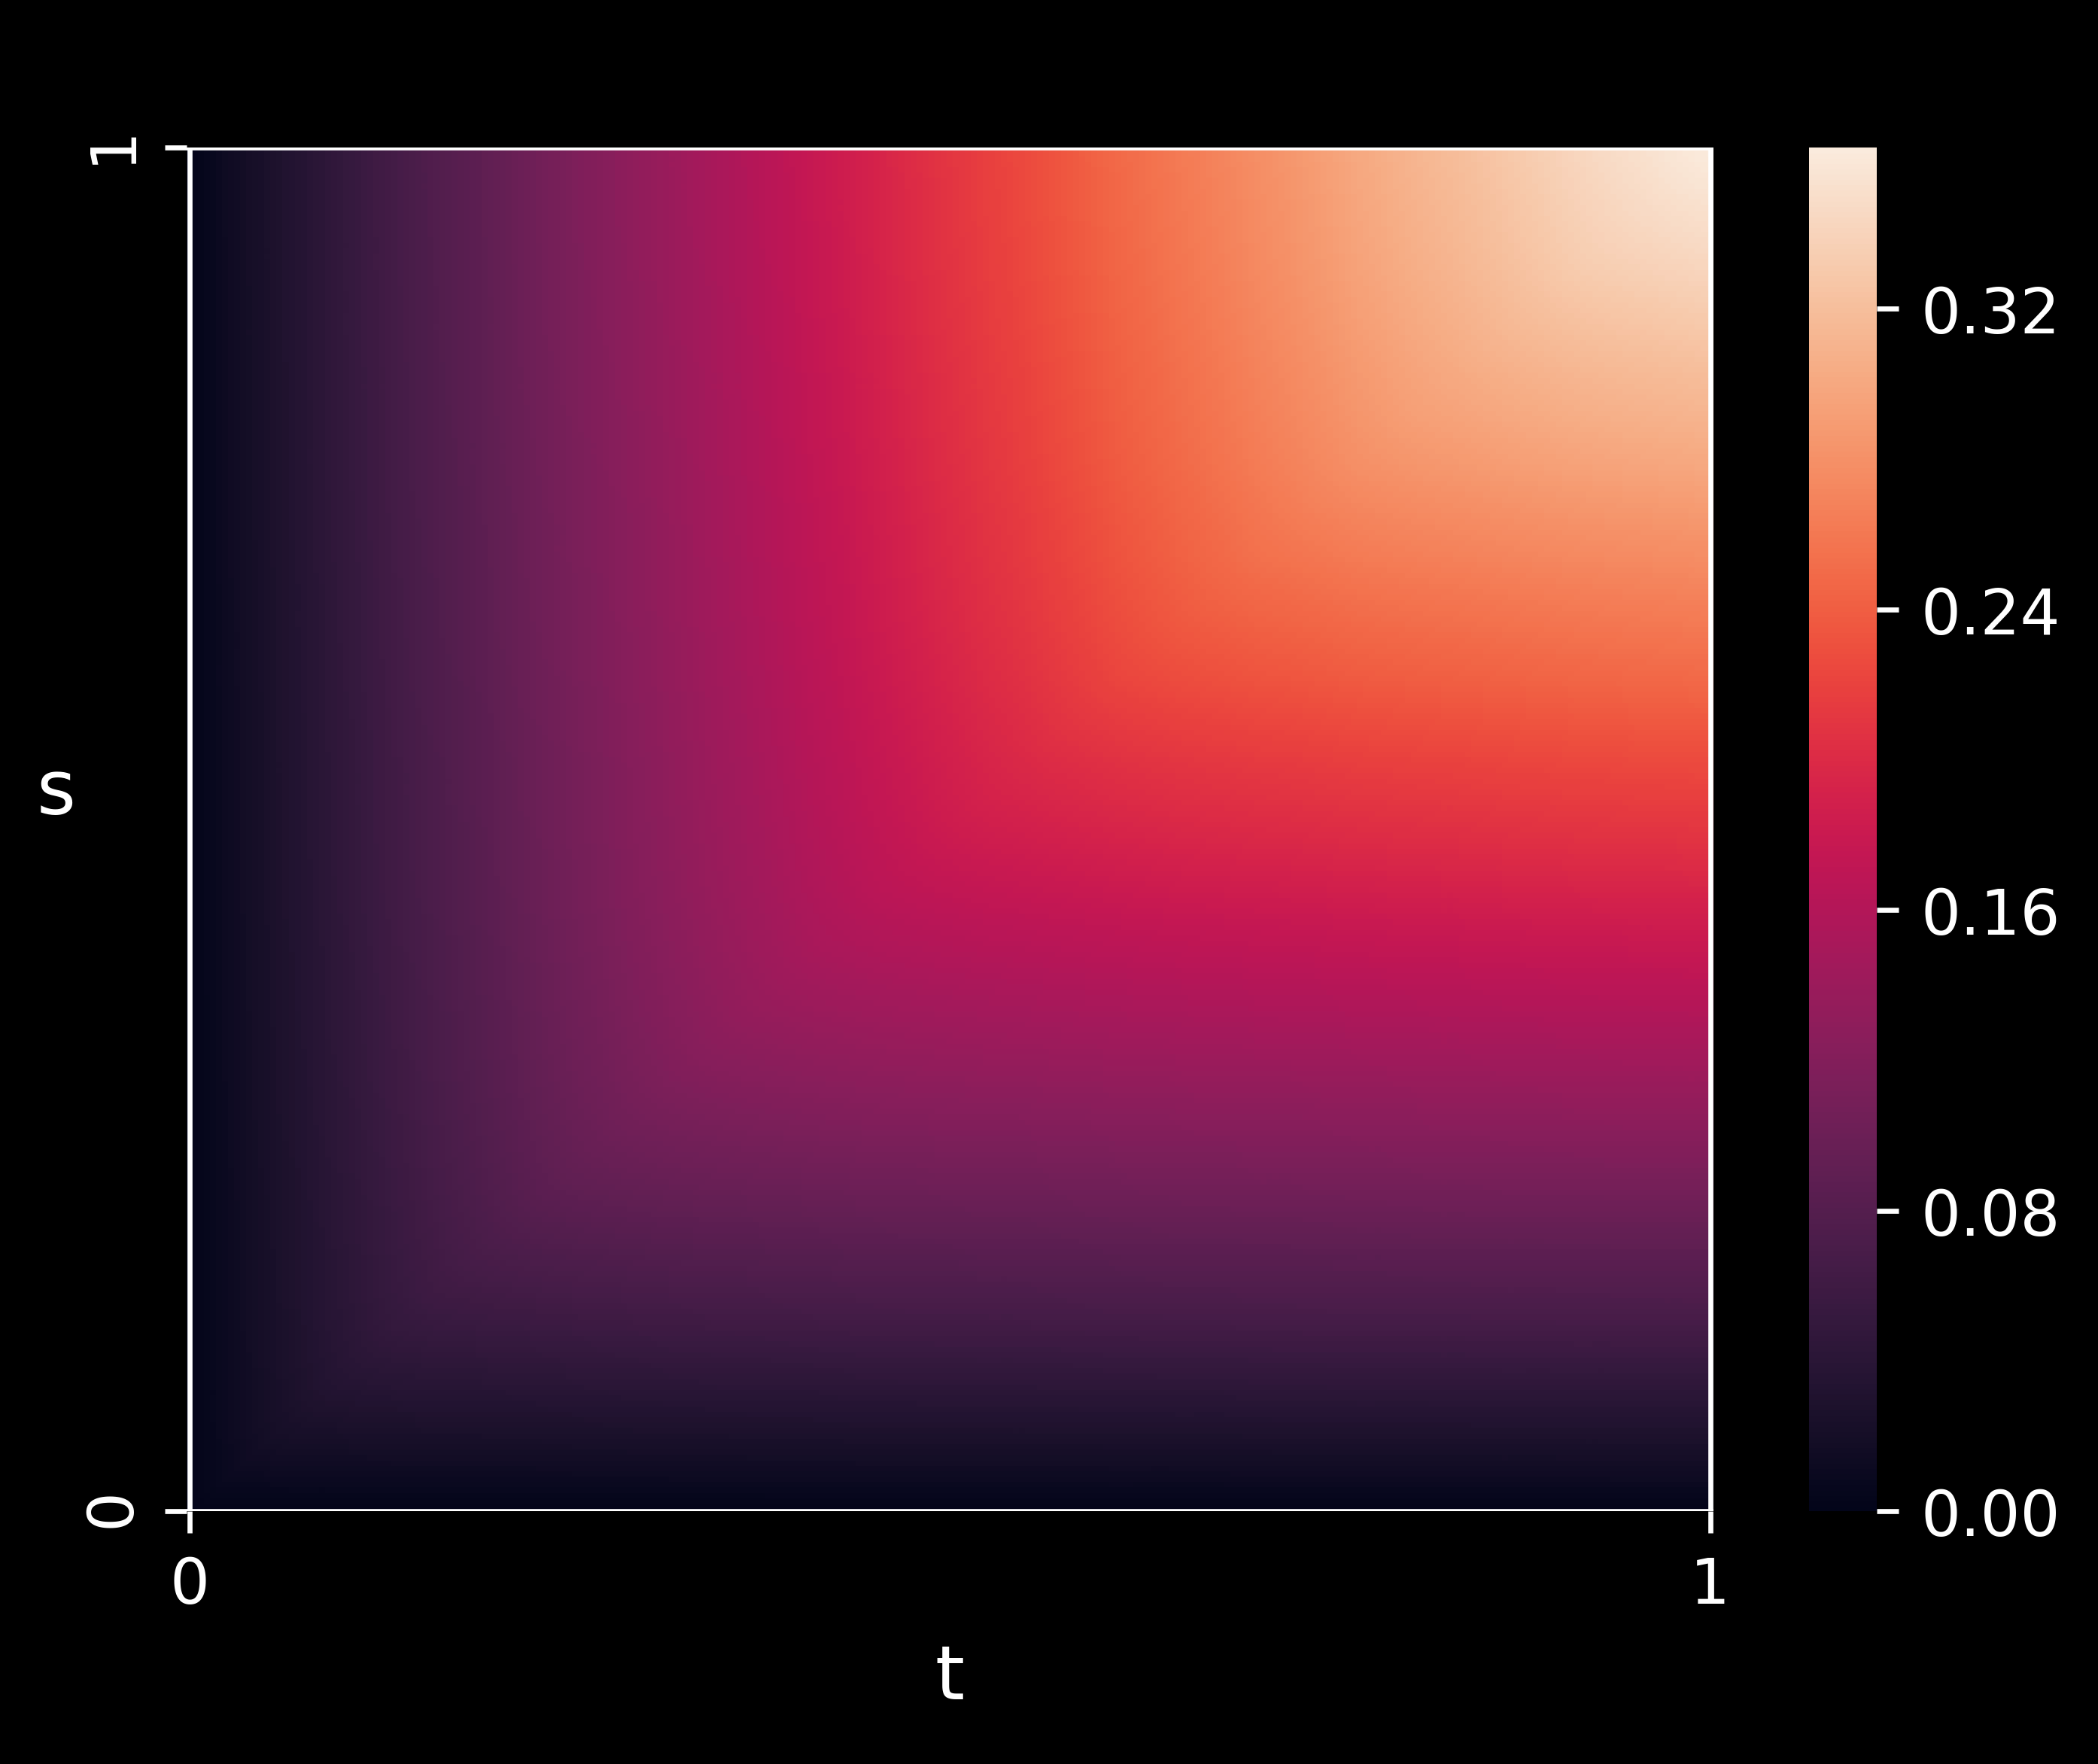
\includegraphics[scale =0.38]{KL/Figures/KLMaximumKernel.png}
    \label{fig:MaxK}
\end{subfigure}
\vspace{2mm}

%\centering
\begin{subfigure}[b]{0.32\textwidth}
    \centering
    %\caption{Time average}
    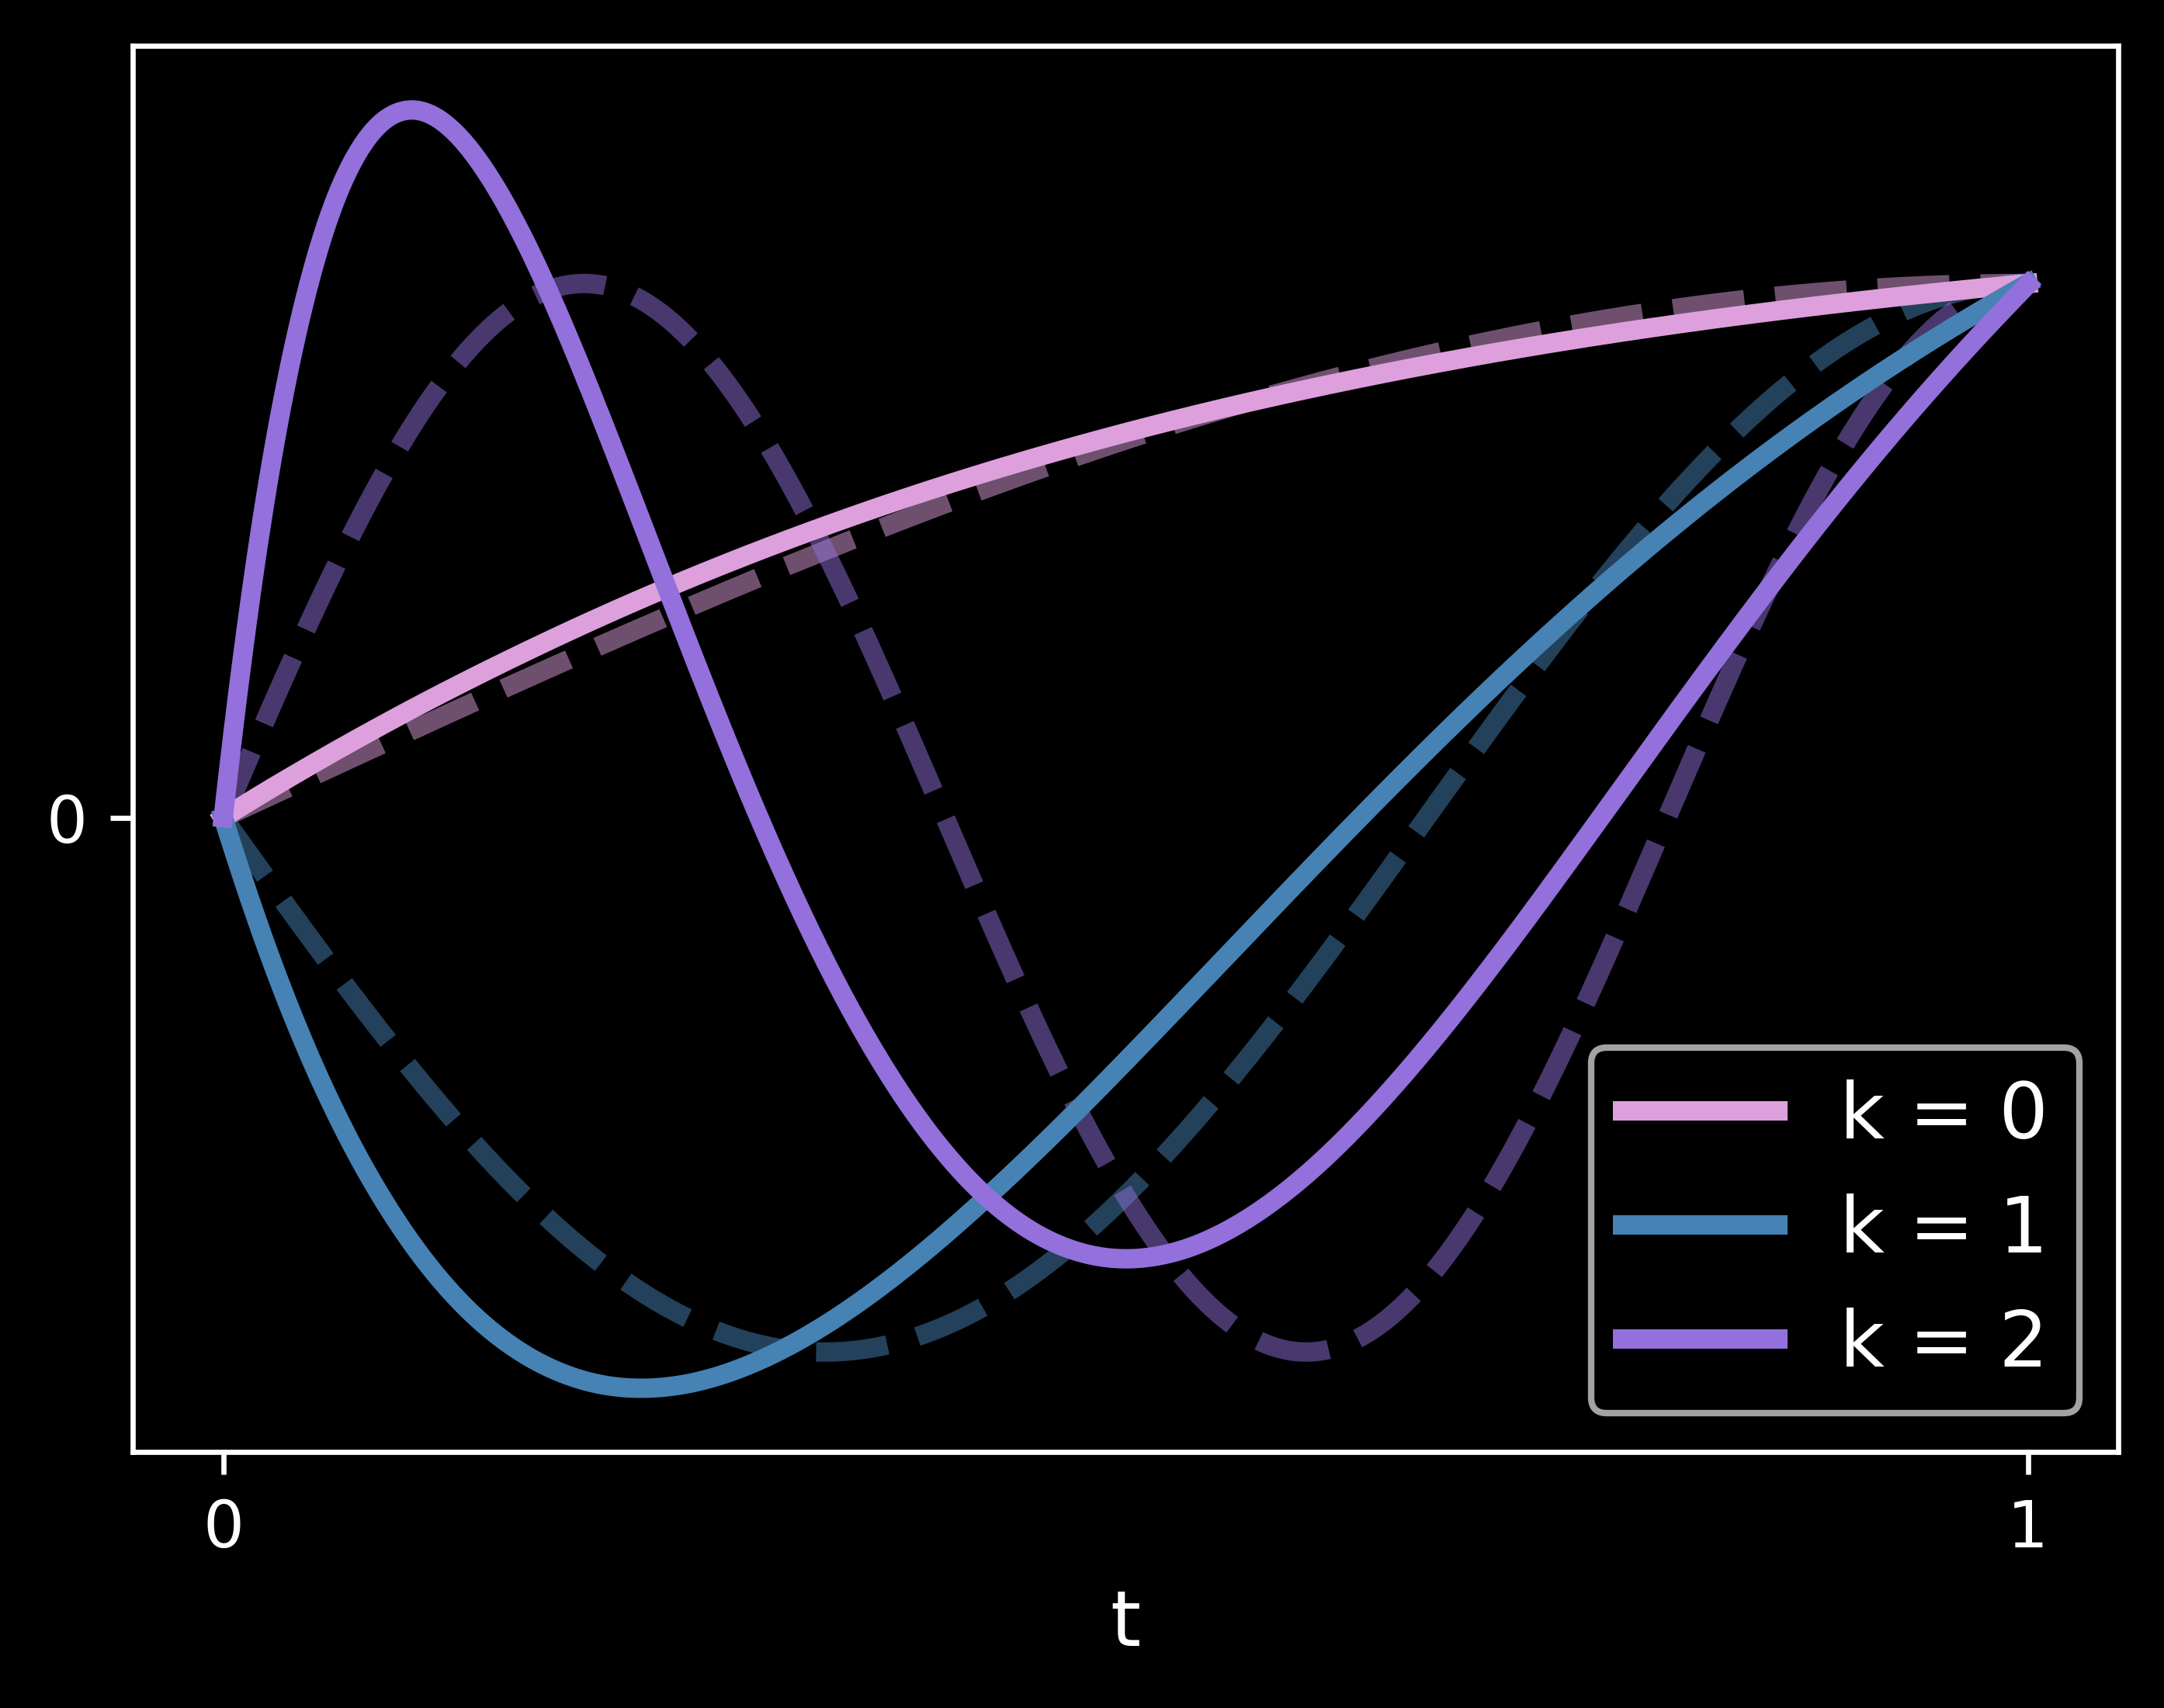
\includegraphics[scale =0.385]{KL/Figures/KLAsian.png}
\end{subfigure}
\begin{subfigure}[b]{0.32\textwidth}
    \centering
    %\caption{Time integral}
    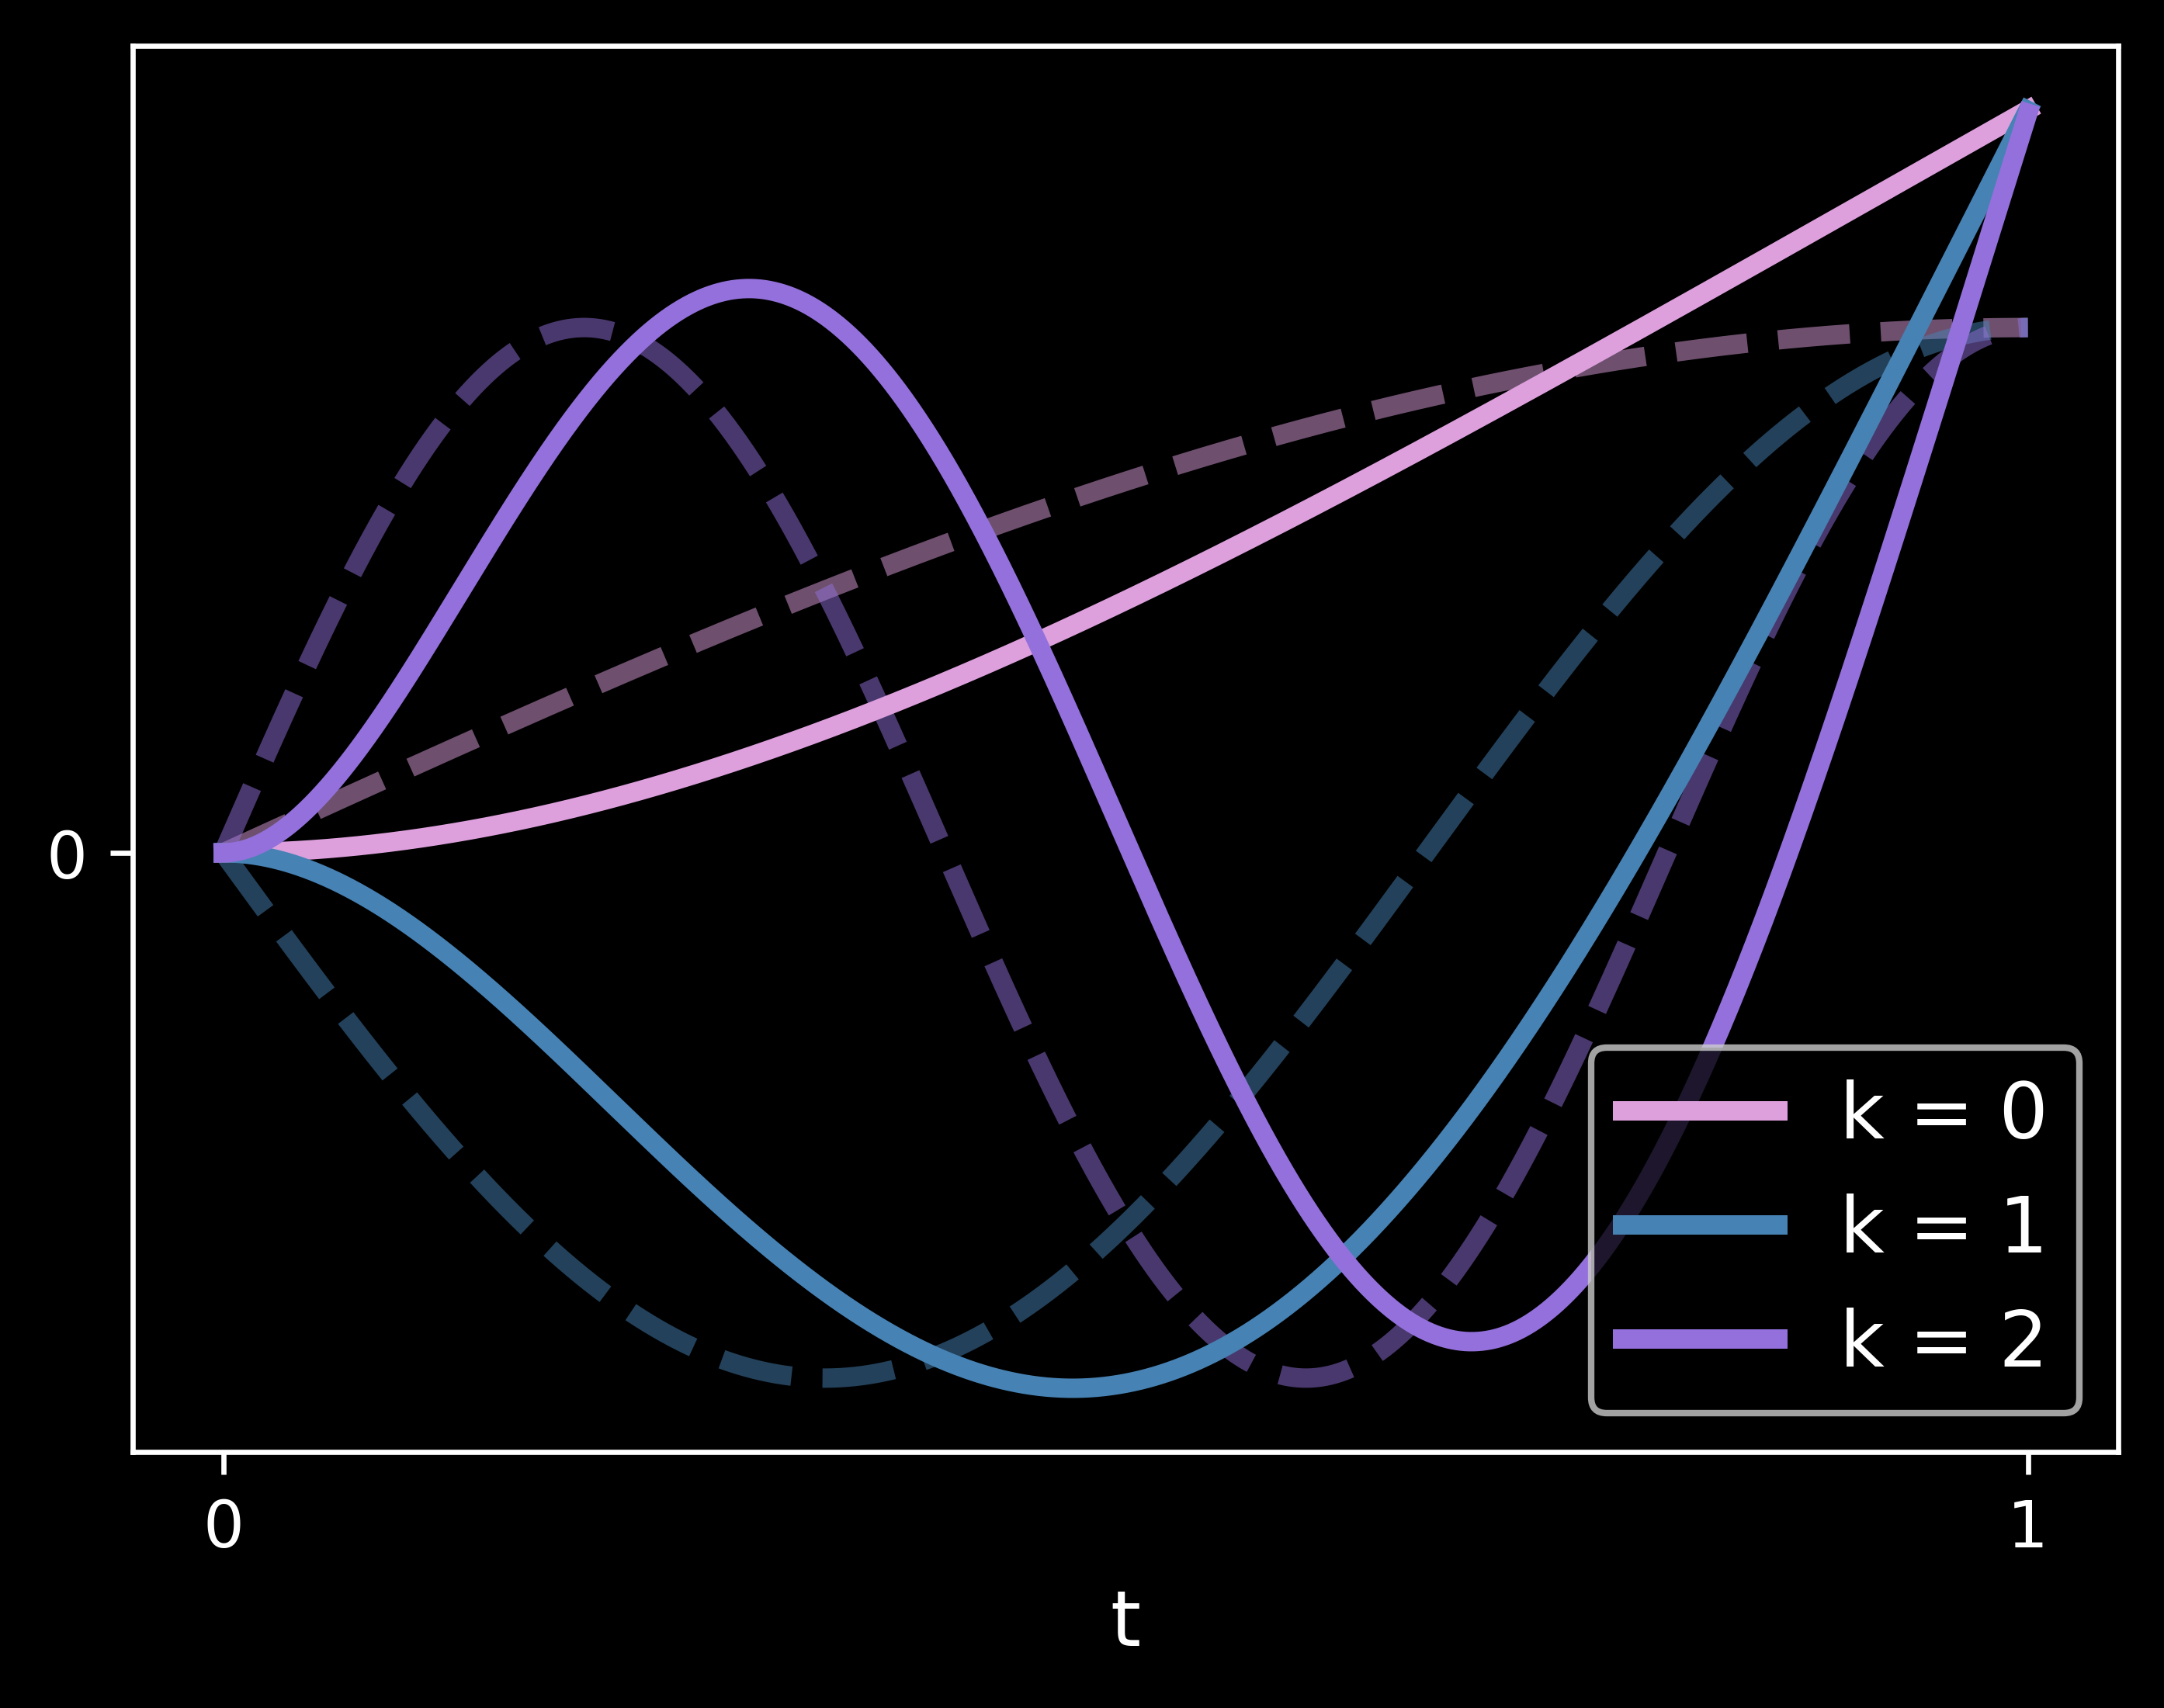
\includegraphics[scale =0.385]{KL/Figures/KLIntegral.png}
\end{subfigure}
\begin{subfigure}[b]{0.32\textwidth}
    \centering
    %\caption{Time integral}
    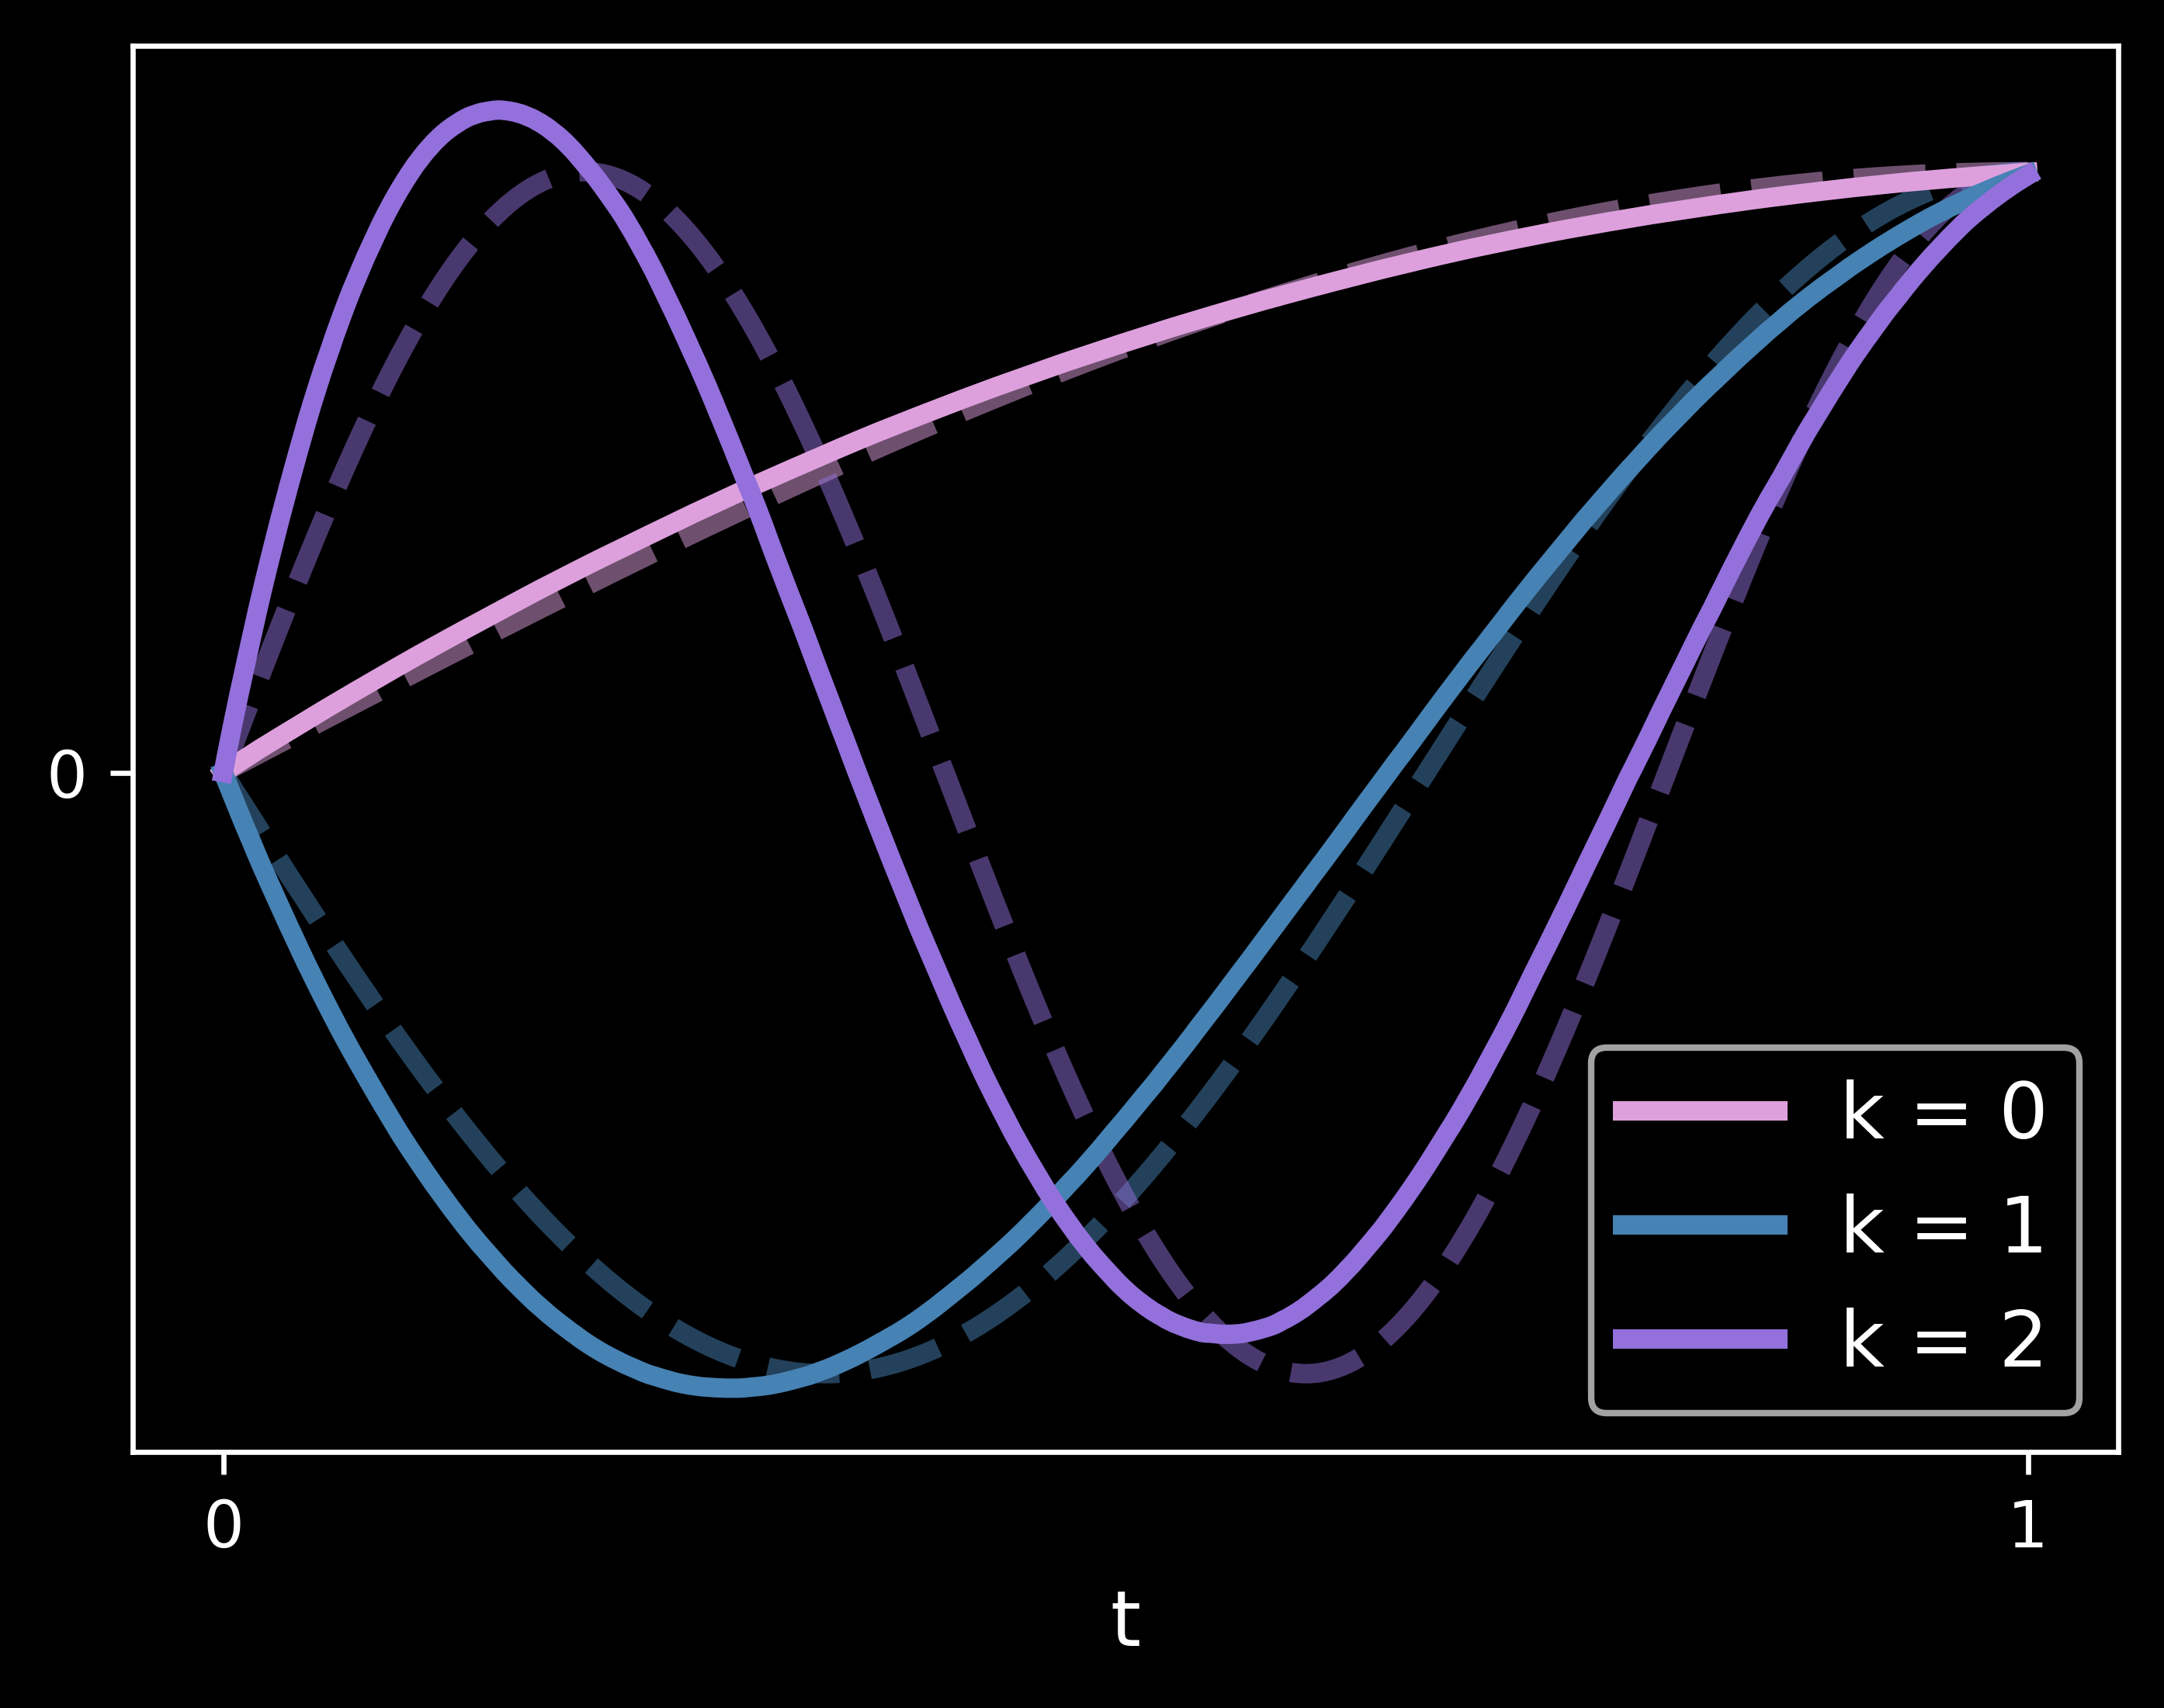
\includegraphics[scale =0.38]{KL/Figures/KLLookback.png}
\end{subfigure}
\vspace{1mm}
\begin{center}
    \footnotesize{
    \textit{Solid lines: transformed
     path.  Dashed lines: Brownian motion.}}
\end{center}
\vspace{-3mm}
\end{figure}

\subsection{Numerical Results} \label{ssec: numResult}
Let us compare the $L^2(\Q \otimes \, dt)$ error  
$\lVert Y^{K,\frakF} - Y \rVert^2_{*} $ in the Brownian case for the two avenues discussed at the beginning of this section. When $Y^{K,\frakF} = (f \circ \pi^{K,\frakF})(X) $, the error is calculated using Monte Carlo simulations. As in  \Cref{sec:numResultX}, we choose $T=1$, $N=10^4$ and $K\in \{1,\ldots,128\}$.  
\Cref{fig:L2Error} displays the result for the running maximum, integral and average functionals. We also add the Brownian motion itself, corresponding to the identity functional $f(X)=X$. We observe a clear improvement when projecting the transformed path. Moreover, it comes as no surprise that smooth functionals (integral, average) exhibits a faster rate of convergence than the running maximum, highly sensitive to local behaviours of a path. 

\begin{figure}%[H]
    \centering
    \caption{$L^2(\Q \otimes dt)$ approximation errors. }
    \vspace{-2mm}
    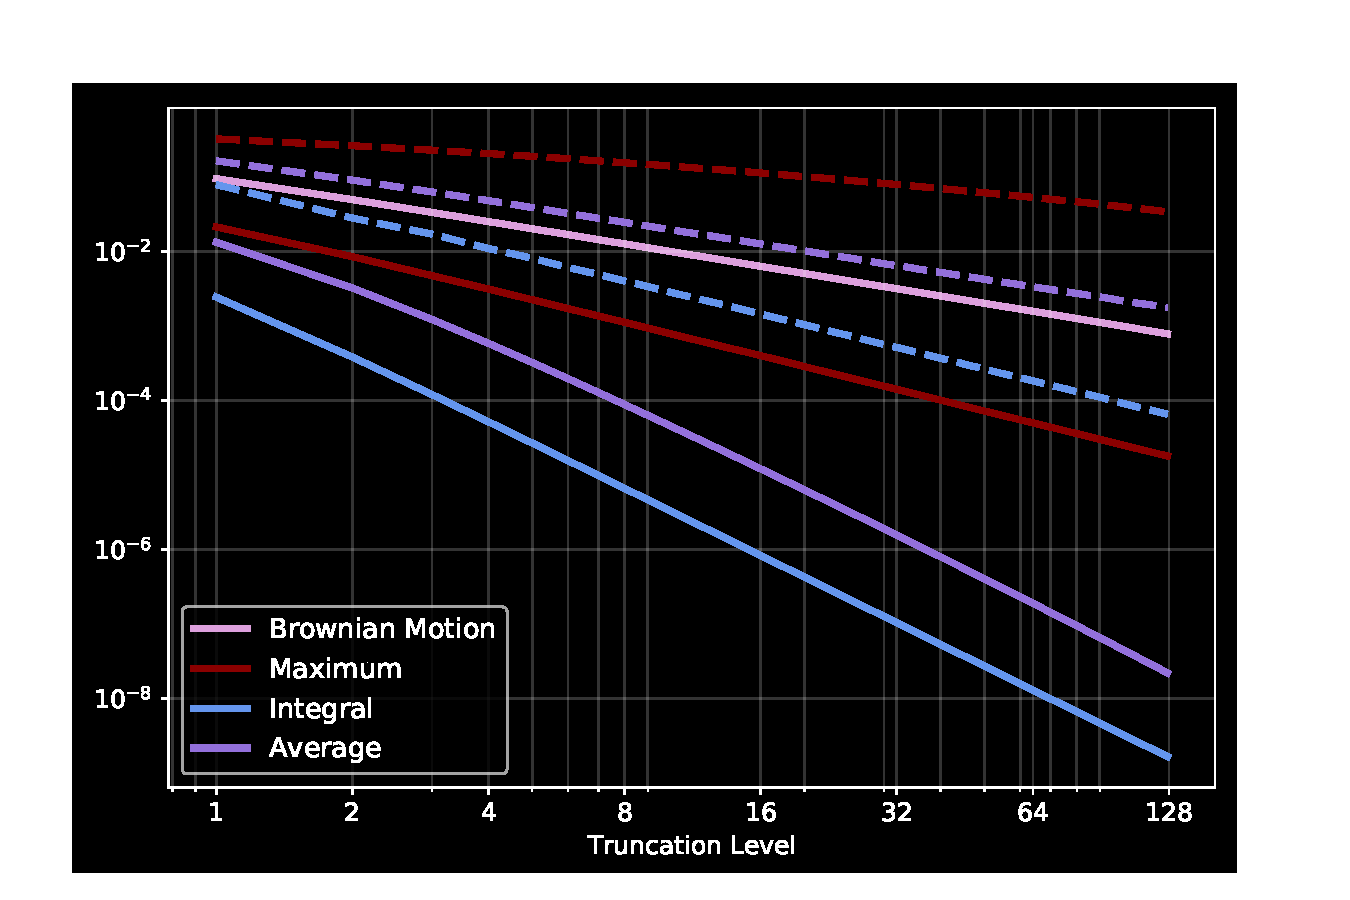
\includegraphics[scale =0.38]{KL/Figures/Error_nSim5000_N1000.pdf}
    \label{fig:L2Error}
    \\
    
    \vspace{1mm}
    
    \footnotesize{
    \textit{Dashed lines: functionals of projected paths. \\Solid lines: projected functionals.}}
\end{figure}

% \subsection{Monotone Convergence}
% When do we have $f_K \nearrow f$? This would ensure, in particular, that 
% $$\lim_{K\to \infty} \E^{\Q}[f_K(X_T)] = \E^{\Q}[f(X_T)].$$ 

% \begin{example}
% (\textbf{Running maximum}) Take 
% $f_K = f \circ \pi^{K,\frakF}$, where $\frakF$ are the Schauder functions and $\calH = \calR$. Then increasing the order $K$ adds new vertices on the graph of $x^{K,F}$ while keeping the ones already there. Hence the maximum, attained on a vertex can only increase. In other words, 
% $$f_K(X_t) = \max_{s\, \le t} x_s^{K,\frakF} = \max_{t_n\, \in \, \Pi_K} x_{t_n}^{K,\frakF} \le \max_{t_n\, \in \, \Pi_{K'}} x_{t_n}^{K',\frakF} = f_{K'}(X_t),
% $$
% if $\Pi_K$ denotes the $K-$th dyadic partition. 

% \end{example}



\subsection{Discussion: Projection of Functionals using the Signature} \label{sec:sigFunc}

Another approximation of $Y=f(X)$ can be obtained by combining  signature functionals in a linear fashion. For instance, one can consider all the words of length less than $\bar{K} \in \N$, giving the approximation
  \begin{equation}\label{eq:sigPayoff}
      y^{K,\calS}_t := \sum_{l(\alpha)\, \le \, \bar{K}} \xi^f_{\alpha} \calS_{\alpha}(X_t), 
  \end{equation}
  \vspace{-3mm}
  
  with $K = |\{\alpha \, | \, l(\alpha)\le \bar{K}\}|=2^{\bar{K}+1}-1.$
  The coefficients $\xi^f_{\alpha}$ may depend on  $X_0$  only and can be  calculated by either regressing  $Y$ against the signature elements or using a Taylor formula for functionals; see \cref{chap:Taylor}.  %\cite{LittererOberhauser} when $f$ is smooth (in the Dupire sense) and $X$ is a diffusion. 
    % In the literature,   $\eqref{eq:sigPayoff}$ is referred to  as  \textit{polynomial functional}  \cite{LittererOberhauser} or \textit{signature payoff} \cite{Szpruch,LyonsNum} in finance. 
     
     The appeal of such projection comes from the fact that polynomial functionals are dense in the space of continuous functionals restricted to  paths of bounded variation; see Theorem 5 in  \cite{LittererOberhauser}.  
     On the other hand, despite the existence of   packages to calculate the signature of discrete time paths (e.g., \texttt{iisignature} and \texttt{esig} in Python), the projection in $\eqref{eq:sigPayoff}$ is still  challenging from a computational perspective. 
     Indeed, contrary to the reconstruction in  \Cref{sec:sigLegendre}, the signature functionals have to be known at \textit{every} intermediate time. Also, as there is a priori no recipe to select words up to a given length,  we must retain all of them so the number of elements doubles every time a layer is added. 



\section{Applications} \label{sec:application}
We now illustrate the benefits of the Karhunen-Loève expansion on functionals for the pricing of exotic derivatives. % written on a single asset. 
We slightly change notations and write $W$ for the coordinate process. The path $X$ now represents the stock price where for simplicity, we employ the Black-Scholes model with zero interest rate. That is,  $\Q$ is the Wiener measure and $x_t = x_0 \calE_t(\sigma  W)$, where $x_0>0$ is fixed and  $\calE$ denotes the stochastic exponential.
Notice, however, that our method applies to any dynamics of the underlying.  

%$\varphi_m(X_t) = (f(X_t)-m\, x_0)^{+}, \, f: \Lambda \to \R,$
%where $m$ is the moneyness of the option. 
%In other words, we restrict ourselves to call options written on a path-dependent quantity of the underlying stock price.  
Let $\calM \subseteq \R$, $\calT \subseteq [0,T]$ be a finite set of option parameters and maturities, respectively. 
We seek to approximate the price surface
$p: \calM \times \calT \to \R$,  $p(m,\tau) = \E^{\Q}[ \varphi_m(X_\tau)]$, where the payoffs  $\varphi_m(X_{\tau}) = (h_m \circ  f)(X_{\tau})$ depends on a parameter $m \in \calM$.  For example, a call option on $Y=f(X)$  is obtained with $h^{\text{Call}}_m(y) := (y-m x_0)^{+}$ and $m$ is the \textit{moneyness} of the option.

The standard Monte Carlo  approach (MC) consists of simulating the underlying path  on a partition  $\Pi_{N} = \{0=t_0 < t_1 < ... < t_N=T \}$  that contains $\calT$ and compute the price as $p^{N,J}(m,\tau) = \frac{1}{J}\sum_{j=1}^J \varphi_m(X^{N,j}_\tau)$, $J\in \N$. 
In contrast, the \textit{Karhunen-Loève Monte Carlo method} (KLMC) samples $Y=f(X)$ directly and computes the price surface  using  the representation $p(m,\tau) = \E^{\Q}[ h_m(y_\tau)]$.  
We now describe the method in more depth. 
\subsection{The KLMC Algorithm}
We assume for simplicity that $Y$ has zero mean, otherwise minor changes  must be made for the KL expansion; see \cref{rem:center}. 
First, we simulate trajectories
$Y^j=(f(X_{t_n}^j))_{t_n \in \Pi_{N_{\text{off}}}}$, $j=1,...,J_{\text{off}}$ with  $J_{\text{off}}, N_{\text{off}} \in \N$,  and compute the eigenfunctions of $\kappa^{N_{\text{off}}}_Y$ as in  $\eqref{eq:eigendecomp}$. Next, for $k=1,...,K$,   we estimate the sample quantile function $\Phi_k^{-1}:[0,1]\to \R$ of $\xi_k = (Y,F_k)$ by employing method N\textsuperscript{o} $\! 7$ in \cite{HyndmanFan}.  
The coefficients $(\xi_k )$ can thereafter be simulated using inverse transform sampling \cite{Devroye}. 
  Notice that these steps can be done in an offline phase so $(\Phi_k^{-1})$ can be reused for other options contingent upon the functional $f$; see \Cref{sec:numResultX}. 
  

In the online phase, we simulate $J \in \N$ transformed paths using inverse transform sampling for $\xi_k$. This gives $y_{\tau}^{K,\frakF,j}= \sum_{k\le K}\xi_k^{j} F_k(\tau)$.  
Finally, the price surface is calculated using Monte Carlo.  The procedure is summarized in \Cref{alg:klmc}. 
It should be noted that although the coefficients $(\xi_k)$ are orthogonal in $L^2(\Q)$, they may well be \textit{dependent} when $Y$ is non-Gaussian. While the marginals of $(\xi_k)_{k\le K}$ are fitted properly, 
the dependence is omitted as generating dependent random vectors with unknown joint distribution is highly non-trivial. Nevertheless, this simplification doesn't induce a bias in the obtained prices as we shall see in the numerical experiments.  


\begin{algorithm}[t]
\caption{(KLMC) }\label{alg:klmc}
\begin{itemize}
\vspace{-2mm}
\item \textbf{Offline}: Given $f$, $K$,  $J_{\text{off}}$, $N_{\text{off}}$ 
\begin{enumerate}
\setlength \itemsep{0.2ex}
\vspace{-2mm}
\item Simulate trajectories $Y^j=(f(X_{t_n}^j))_{t_n \in \Pi_{N_{\text{off}}}}$, $j=1,...,J_{\text{off}}$
\item Compute $\kappa^{N_{\text{off}}}_Y$ (closed-form or from the sample  $(Y^j)$)
\item Solve the eigenvalue problem $\eqref{eq:eigendecomp}$ to obtain  $(\lambda^{\frakF}_k,F_k)$
\item Using $(Y^j)$, estimate the quantile functions  $\Phi_k^{-1}$, $k\le K$ 
\end{enumerate}
\vspace{-2mm}

\item \textbf{Online}: Given $J, \ \calM, \ \calT$ 
\begin{enumerate}
\setlength \itemsep{0.2ex}
\vspace{-2mm}
\item Simulate $\xi^j_k = \Phi^{-1}_k(u_k^j)$, $(u_k^j) \overset{i.i.d.}{\sim} U(0,1)$, $j \le J$, $k\le K$
\item Compute $y_\tau^{K,\frakF,j} =\sum_{k=1}^K  \xi^j_k    F_k(\tau)$, $\tau \in \calT$, $j\le J$ 
\item Estimate the price surface $p^{K,\frakF,J}(m,\tau) := \frac{1}{J}\sum_{j=1}^{J} h_m(y_\tau^{K,\frakF,j}).$
\end{enumerate}
\end{itemize}
\vspace{-3mm}
\end{algorithm}

\subsection{Numerical Results} \label{sec:numResultPrice}
First, we build the price surface for  Asian and lookback call options, i.e. by choosing $h_m = h^{\text{Call}}_m$ and the running maximum and time average as underlying functional, respectively. Of course, the put option price surface can  be retrieved thanks to  put-call parity. We also consider Up \& Out digital options, that is $f(X_t)=\max_{0\le s \le t}x_s$  and   $h^{\text{UO}}_m(y):=\mathds{1}_{\{y \ \le \ m x_0\}}$. The parameter $m\ge 1$ thus represents the barrier of the option relative to the spot price. 
We can therefore reuse the quantile functions computed for the lookback call options.

The parameters are $(x_0,\sigma,N_{\text{off}},J_{\text{off}},J) = (100, 0.2, 10^3, 2^{17}, 2^{19})$, 
 $T=1$ year and $\calT =  \{\frac{1}{52},\frac{2}{52},\ldots,1\}$ (weekly maturities). 
The moneyness and barrier levels are respectively $\calM^{\text{Call}} = \{0.75,0.80,\ldots,1.25\}$ and $\calM^{\text{UO}} = \{1.05,1.10,\ldots,1.50\}$. 
We assess  accuracy  in the mean square sense, namely by computing 
$$
\text{MSE} =  \frac{1}{|\calM|\ |\calT|}\sum_{(m,\tau) \in \calM \times \calT} |p^{\text{(B)}}(m,\tau) - \hat{p}(m,\tau)|^2. 
$$ The function $\hat{p}$ is the approximated price and $p^{\text{(B)}}$ a benchmark obtained using a standard Monte Carlo with $40 \cdot |\calT| = 2080$ time steps and same number of simulations. 
\interfootnotelinepenalty=10000 
  \cref{tab:results} displays the MSE, runtime (online phase) and number of variates per simulated path ($K$ and $N$ for the KLMC and MC method, respectively).\footnote{The experiments have been made on a personal computer; see \href{https://github.com/valentintissot/KLMC.git}{https://github.com/valentintissot/KLMC} for an implementation. The offline phase takes about 10 seconds per  functional.}  Notice that we increase $K,N$  for the lookback call and Up \& Out digital option as the running maximum has a slower rate of $L^2(\Q\otimes dt)$ convergence  as seen in \Cref{fig:L2Error} for the Brownian case.  The KLMC method constantly yields a lower MSE and runtime.  For the Asian call option, note that the number of variates per path is less than the number of maturity points and KLMC method, which couldn't be done with the MC method. 
  
 \vspace{-1mm}

\begin{table}[H]
    \centering
\caption{Mean squared errors and runtime (seconds)}
\vspace{-3mm}
\begin{tabular}{ccccccc} 
\hline  & \multicolumn{3}{c}{KLMC}  & \multicolumn{3}{c}{MC} \\  \hline
Option & K & MSE  & Time & N & MSE & Time \\
\hline  
 Asian Call & $40$ & 1.50e-04 & 2.26 & $ 52$ & 3.10e-04 & 2.40\\ 
Lookback Call   & $100$ & 1.15e-02 & 4.47& $4\cdot 52$ & 1.92e-01 & 7.05 \\ 
Up \& Out Digital   & $100$ & 1.80e-04 & 4.40 & $4\cdot 52$ & 1.90e-04 & 6.88\\ \hline
\end{tabular}
\label{tab:results}
\end{table}

\section*{Conclusion}
We shed further light on the approximation of path functionals. After a  review of Hilbert projections and a connection with the path signature, we show the power of the Karhunen-Loève expansion to parsimoniously simulate path-dependent payoffs. 
Further work would include the use of copulas in the  KLMC algorithm to capture the dependence between the $L^2([0,T])$ coefficients of the Karhunen-Loève expansion and a performance comparison with signature-based methods. 

%\bibliography{KL/ref.bib}

%\chapter{Path-Dependent Claims: The Functional Taylor Expansion}\label{chap:Taylor}

%========= Intro ==========%
%\section*{Introduction}


The stochastic Taylor expansion  \cite{KP} %[Chapter~5] 
 lies at the core of numerical 
 integration of 
 stochastic differential equations.
It provides explicit weak/strong 
error bounds for discretization
schemes, which is of great relevance for the valuation of European derivatives. %, e.g. Euler-Maruyama, Milstein-Platen, to name a few.
 %It permits the construction of numerical schemes where the approximation error (weak or strong) can be made explicit. 
 %It seems therefore natural to extend this tool to the framework of path-dependent functionals. 
% For instance, the Monte Carlo pricing error with trajectories from the Euler schemes  is controlled by the step size of the discretization in a linear fashion.
% In the valuation of European options, the Euler-Maruyama scheme yields a pricing (or weak) error proportional to the step size of the discretization. For path-dependent payoffs, one is rather interested in the hedging (or strong) error of a numerical method.
%For instance, the Euler-Maruyama method (\cite{Maruyama}) yields a pricing/weak error for power options that is proportional to the discretization step size.
For instance, the Euler-Maruyama method \cite{Maruyama} yields a weak error for the expectation of monomials %—or in financial terms, the price of European power options—
that is proportional to the time step.  %discretization step size. %In financial terms, this means that power options are priced 
By extension, it seems natural to seek %look for 
test functionals akin to monomials which characterize weak convergence for path-dependent payoffs. 

A good candidate is the family of \textit{signature functionals}. The path signature has gained much attention in recent years, due in particular %to its  ability to compress a path efficiently and 
to its universal approximation property \cite{LyonsNum,Szpruch}. In fact, a density result à la Stone-Weierstrass exists \cite{Hao}. %for these functionals,
In light of this, the signature functionals
plays therefore the role of monomials in the path space. %therefore 
This parallel is further reinforced %also
%apparent
in cubature methods \cite{LyonsVictoir,Crisan}   generalizing Gaussian quadrature rules to the Wiener space; %orthogonal polynomials %whose integral must match under a discrete measure 
%are replaced by signature elements.
the exact integration of orthogonal polynomials 
turns into a perfect fit of expectated signature elements. \bb{+ \ldots}
%under a discrete measure 
% boils down to matching expectation of signature elements. turns into a perfect fit of expectated signature elements.

%becomes a moment matching condition for signature elements. %whose integral must match under a discrete measure 
%are replaced by signature elements.

%The matching of integrals 
%  matching the expectation of signature elements under the Wiener measure. 
 
%In this paper
In response to this appeal, % these challenges, 
we shed further light on the stochastic Taylor expansion for  path-dependent payoffs, which we call the \textit{functional Taylor expansion}. %Without much surprise, 
This is made possible by 
tools from the functional Itô calculus \cite{Dupire}. To the best of our knowledge, this generalization has been first proposed by \cite{LittererOberhauser} %where the underyling path is 
in the diffusion case.    
In this is work, we intend to bring  clarity to this deep result and establish a parallel with the Wiener-chaos expansion \cite{DiNunno,Nualart}. 
%\bb{+\ldots}


%Fréchet (Hille-Phillips) vs Functional Itô expansion? 

%We believe that this connection will help the reader 
%to further gain intuition into this beautiful yet technical result.
% in a natural framework.
%Due to their density property, the signature functionals play the role of the monomials in the space of functionals.

%The remainder of this work is organized as follows. \bb{...}

 
   
 
%  \bb{Cubature:} Lyons-Victoir, Crisan, Filipovic et al. (towards American options).
%========= Section 1 ==========%
\section{The Functional Taylor Expansion}

%\subsection{Functional It\^o Calculus}
We fix throughout a horizon $T>0$, which can be interpreted as the maturity of a financial derivative. Let $\Lambda_t = \calD([0,t],\R)$ be the Skorokhod space of c\`adl\`ag paths of length $t\in [0,T]$. 
Given $X_t\in \Lambda_t$, $X_s$ denotes the whole trajectory up to time $s\le t$, while $x_s= X_t(s)$ is the value at time $s$. 
Moreover, write $\Lambda := \bigcup_{t\in[0,T]}\Lambda_t$ for the collection of all c\`adl\`ag paths. The distance between elements of $\Lambda$ is measured according to %can  and define the metric
$$d_{\Lambda}( X_t, Y_s) =t-s + \sup_{0 \le u \le t} |x_u - y_{u\wedge s} | , \quad 0 \le s \le t \le T. $$ %\lVert X_t - Y_{s,t-s} \rVert_{\infty}
%the flat extension $X_{t,\delta t}(s) = x_{s \wedge t}$, $s\in [0,t+\delta t ]$. 
See \cite{Dupire} for other topological considerations. % on the topology of $\Lambda$.  
We adorn $\Lambda$  %with a $\sigma-$algebra $\calF$, filtration $\F$ and probability measure $\Q$ %(e.g., the Wiener measure) 
%to form 
with a stochastic basis
$(\Lambda,\calF,\F, \Q)$. %With a slight abuse of notation, w
We interpret $X \in \Lambda$ both as a path and the coordinate process. To disambiguate the notations, we will often use the letter $X$ when referring to a  specific path and $Y$ when taking (conditional) expectation under $\Q$. %for the (random) coordinate process% where $\calF$ is the natural filtration of the coordinate process $X_t(\omega)=\omega_t$

A \textit{functional} transforms a path into a scalar, i.e. it is a map $f:\Lambda \to \R$. We make the distinction between functionals defined on $\Lambda$ and those restricted to trajectories of maximal length, i.e. $g:\Lambda_T \to \R$. The latter are called \textit{$T-$functionals}.  
%Lastly, we introduce important classes of functionals. 
For $p\in [1,\infty]$ and $t\in [0,T]$, 
let $L^p(\Lambda_t)$ be the subspace of functionals $f$ restricted to $\Lambda_t$ such that  
\begin{equation}\label{eq:L(Lambda_t)}
    \lVert f \rVert_{L^p(\Lambda_t)} :=  \lVert f(Y_t) \rVert_{L^p(\Q)} < \infty.
\end{equation}
Furthermore, we define 
\begin{equation}\label{eq:L(Lambda)}
    L^p(\Lambda) = \left \{ f: \Lambda\to \R \ \Big | \ \lVert f \rVert_{L^p(\Lambda)} := \sup_{t \in [0,T]} \lVert f \rVert_{L^p(\Lambda_t)} < \infty \right\}
\end{equation}
 Clearly, $f\in L^p(\Lambda) $ implies that $f|_{\Lambda_t} \in L^p(\Lambda_t)$ for all $ t \in [0,T]$. The converse is  false in general, as shown by the deterministic functional $f|_{\Lambda_t}  \equiv \frac{1}{t}\mathds{1}_{\{t>0\}}$. The interested reader may verify that $\lVert \cdot \rVert_{L^p(\Lambda)}$ is a norm and $L^p(\Lambda)$ a Banach space. % \bb{(?)}.

%In essence, the functional Taylor expansion separates the idiosyncratic

%\subsection{Path Signature}

%We now recall the concept of path \textit{signature}.

\subsection{Path Signature} 
We briefly recall the definition of the signature (see \cref{sec:sigLegendre})  which is here defined for  c\`adl\`ag  paths.%  which is central in the functional Taylor expansion. 
%The expansion of functionals entails a collection of objects that characterizes the underlying path in its entirety. This is given by the \textit{signature}, which can be seen as the infinite
%skeleton of a path. %, where  each "bone" contains inherent information.  
% A key ingredient in the expansion of functionals is the \textit{path signature}. In essence, the signature extract  from a path an infinite-dimensional skeleton, where  each "bone" contains inherent information about a trajectory. 
%We start off with a few definitions. 
A \textit{word} is a sequence  $\alpha = \alpha_1 \ldots \alpha_k$ of letters %(or indexes) 
from the alphabet $\{0,1\}$.  The number of $0$'s and $1$'s contained in $\alpha$ is denoted by $|\alpha|_0$, $|\alpha|_1$, respectively. The \textit{length} of $\alpha$ is therefore $|\alpha| := |\alpha|_0 + |\alpha|_1$. We will often use the special words $\boldsymbol{0}_k := \underbrace{0\ldots 0}_{k}$ and $\mathds{1}_k := \underbrace{1\ldots 1}_{k}$.
%When $|\alpha|_0 = |\alpha| = k$ ($|\alpha|_1 = |\alpha| = k$), we simply write $\alpha = \boldsymbol{0}_k$).  % and define $\calA_k = \{\alpha \, | \, l(\alpha) = k\}$ ($\calA_0 = \emptyset$). 

%For reasons explained later, 
We enlarge a path $X \in \Lambda$ with the time itself %$t \mapsto t$  
and henceforth set %, with a slight abuse of notation,
$x^0_{t} = t$, $x^1_{t} = x_t$.  The indexes $0,1$ are therefore identified with the time $t$ and path $x$, respectively.  
% If   $f: \Lambda \to \R$ is an $\Q-a.s.$ integrable functional and $B$ a Borel set of $[0,t]^k$, we employ the compact notation 
% $$\int_{B} f(X_{t_1}) \circ \, dx^{\alpha} = \int_{[0,t]^k} f(X_{t_1}) \mathds{1}_{B}(t_1,\ldots,t_k)\circ \, dx^{\alpha_1}_{t_1} \cdots \circ dx^{\alpha_k}_{t_k}.$$
%  The symbol $\circ$ indicates that when $X$ is a  semimartingale, the integral is in the sense of Stratonovich. For trajectories with finite variation $\Q-a.s.$, the latter boils down to a Riemann-Stieltjes integral. 
 
 \begin{definition}\label{def:Sig}
     The \textit{signature in $\Lambda$} is a collection  of functionals $\calS = \{\calS_{\alpha}: \Lambda \to \R\}$ such that
     \begin{align*}
     \calS_{\emptyset}(X_t) &= 1, \\
         \calS_{\alpha}(X_t) &= \int_{\triangle_{k,t}} \circ \, dx^{\alpha} =\int_{0}^{t} \int_{0}^{t_k} \cdots \int_{0}^{t_2} \circ \, dx^{\alpha_1}_{t_1} \cdots \circ dx^{\alpha_k}_{t_k}, \quad |\alpha|=k,
     \end{align*}
     for  the simplexes $\triangle_{k,t}= \{(t_1,\ldots,t_k)\in [0,t]^k\,|\, t_1 \le \ldots \le t_k\}$, $\, k\ge 1$.  The circle $\circ$ denotes Stratonovich integration. 
 \end{definition}
% Observe that integrals in  \Cref{def:Sig} are in the Riemann-Stieltjes sense when either the integrand or integrator is of bounded variation. In such situation, the symbol $\circ$ is omitted. 
% The first signature functionals read
% \begin{align*}
%     \calS_{0}(X_t) &= \int_0^t d t_1 = t, &&\calS_{1}(X_t) = \int_0^t \circ \,d x_{t_1} = x_t - x_0,\\
%   \calS_{00}(X_t) &= \int_0^t \int_0^{t_2} d t_1 d t_2 =\frac{t^2}{2}, &&\calS_{01}(X_t) = \int_0^t \int_0^{t_2} d t_1 d x_{t_2} =\int_0^t (x_{t} - x_s) ds, \\
%   \calS_{10}(X_t) &= \int_0^t \int_0^{t_2} dx_{t_1}  d t_2 =\int_0^t (x_{s} - x_0) ds, &&\calS_{11}(X_t) = \int_0^t \int_0^{t_2}\circ \, d x_{t_1} \circ d x_{t_2}=\frac{(x_t-x_0)^2}{2},
% \end{align*}
% or hierarchically,% representation,
% % A hierarchical representation of the signature is given by the following infinite tree, 
% \begin{align}\label{eq:tree}
%   \begin{pmatrix} 
% & &  \calS_{\emptyset}& &  \\
% &  \calS_{0} & &   \calS_{1} &\\
% \calS_{00} &    \calS_{01} & &  \calS_{10}  & \calS_{11}\\
% \vdots & \vdots & &\vdots & \vdots
%  \end{pmatrix} \;=\; \begin{pmatrix} 
% & &  {1} & &  \\
% &  {t} & &  {x_t} &\\
% {\frac{t^2}{2}} &  
% {\int_0^t s \, dx_s} & & {\int_0^t x_s ds} & {\frac{x_t^2}{2}}
%  \\
% \vdots & \vdots & &\vdots & \vdots
%  \end{pmatrix}.
%  \end{align} 
% As can be seen, 
% each entry %in the above infinite pyramid 
% generates two descendants by either integrating the former with respect to $t \sim 0$ or $x \sim 1$. 
It is important to note that  $\calS_{\alpha}$ may not be well-defined for all paths in $\Lambda$. We can thus define the \textit{domain} $\calD_{\alpha} \subseteq \Lambda$ of the signature functional associated to $\alpha$. The stochastic basis  naturally plays a role here. For instance, $\calD_{11}$ is the topological support of all $(\Q,\F)-$semimartingales so that the Stratonovich integral is well defined. 
%For instance % time or the path. %($0$) or the path ($1$).

% The signature is a fascinating object with many questions still to be adressed: Are the signature functionals linearly independent? Do they form a basis? If yes, in which sense? We easily see that for  fixed time point, say $t\in [0,T]$, the signature elements are linearly dependent. For instance, using integration by parts,
% $$\calS_{10} + \calS_{01}= \int_0^t x_s ds + \int_0^t s dx_s  = t \, x_t= \calS_{0}\calS_{1}.$$
% With $t$ known, it can be treated as a coefficient, implying that $\calS_1, \calS_{01}, \calS_{10}$ are linearly dependent. However, when the signature elements are seen as  (running) functionals, they become linearly independent. 

%Another interesting 

% The signature can also be represented as an infinite tree, where each node generates two leaves by either integrating it w.r.t. time or the path itself:

% \begin{align*}
%  \begin{pmatrix} 
% & &  \calS_{\emptyset} & &  \\
% &  \calS_{0} & &  \calS_{1} &\\
%  \calS_{00} &   \calS_{01} & & \calS_{10} & \calS_{11}\\
% \vdots & \vdots & &\vdots & \vdots
%  \end{pmatrix}
% \end{align*} 

% Keeping track of the passage of time  is crucial. Otherwise, the signature would bear barely any information about the path. Indeed, notice that
% $\calS_{\alpha}(X_t) = \frac{(x_t-x_0)^{k}}{k!}$ for  $\alpha =  1...1$ %\underbrace{1...1}_{k}$
% , $|\alpha| = k$. In the alphabet $\{1\}$, the signature would therefore only characterizes the ditribution of $x_T$, or in financial  terms, the volatility smile.
\subsection{Functional Itô Calculus}
  The concepts of spatial and temporal derivative for functionals (\citet{Dupire}) are now recalled. 

\begin{definition}
Let $X \in \Lambda$ and $f:\Lambda \to \R$ be a functional. Assuming existence of the following quantities, we define
\begin{itemize}
    \item The \textit{spatial derivative},
    $$\Delta_x f(X_t) = \lim_{\delta x\to 0} \, \frac{f(X^{\delta x}_t)-f(X_t)}{\delta x}, $$
    with the bumped path $X^{\delta x}_t(s) =  x_s + \delta x\,\mathds{1}_{\{s\,=\,t\}}$, $s\in [0,t]$.
     \item The \textit{temporal derivative},
    $$\Delta_t f(X_t) = \lim_{\delta t\downarrow 0} \, \frac{f(X_{t,\delta t})-f(X_t)}{\delta t},$$
    with the flat extension $X_{t,\delta t}(s) = x_{s \wedge t}$, $s\in [0,t+\delta t ]$. %$X_{t,\delta t}|_{[0,t]} = X_{t}$, $X_{t,\delta t}|_{[t,t+\delta t]} \equiv x_{t}$.
\end{itemize}
\end{definition}
Multiple derivatives are denoted by  $\Delta_{\alpha} = \Delta_{\alpha_1} \cdots \Delta_{\alpha_k}$. For instance, 
$\Delta_{101}f = \Delta_{x} (\Delta_t(\Delta_x f))$, where we stress again that  $0,1$ is identified with $t,x$, respectively. Besides if $\alpha = \emptyset$, then $\Delta_{\alpha}$ is the identity operator.

A crucial remark is that $\Delta_x$ and $\Delta_t$ do not commute. Put another way, the \textit{Lie bracket},
$[\Delta_x,\Delta_t]f := \Delta_{xt}f- \Delta_{tx}f$ is in general non-trivial. See Example \ref{ex:QV}. The Lie bracket provides an instantaneous path-dependence gauge, as explained in  \cite{Jazaerli}. 
%In particular, a functional $f$ that satisfies $[\Delta_x,\Delta_t]f=0$ is called \textit{locally weakly path-dependent}.  

\begin{example}\label{ex:IntDev}
We compute the functional derivatives of the time integral $f(X_t) = \int_0^t \varphi(X_s) ds$.
Since $\{ s\in [0,t] \, | \, X_t(s) \ne X^{\delta x}_t(s)\} = \{ t \}$ has Lebesgue measure zero, we conclude $\Delta_xf \equiv 0$. For the time derivative, we simply obtain  
    \begin{align*}
        \Delta_t f(X_t) &= \lim_{\delta t\downarrow 0} \,  \frac{1}{\delta t}\int_t^{t+\delta t} \underbrace{X_{t,\delta t}(s)}_{= \, x_t}  ds = x_t.
    \end{align*}
\end{example}

\begin{example}\label{ex:QV} Consider the quadratic variation functional, namely
$$\langle X \rangle_t =  \lim_{N \to \infty} \sum_{t_i\, \in \, \Pi_{N}} (x_{t_i}-x_{t_{i-1}})^2,$$
where $(\Pi_N) = (\{0 = t_0 < \ldots < t_N = t\})$ is a sequence of refining partitions of $[0,t]$.
First, the time derivative of $f$ is nil as a flat-extension  does not provide additional variation. On the other hand, the space derivative reads
\begin{align*}
    \Delta_x \langle X \rangle_t &= \lim_{\delta x \to 0} \frac{\langle X^{\delta x} \rangle_t-\langle X \rangle_t}{\delta x} = \lim_{\delta x \to 0} \lim_{N \to \,\infty} \frac{(x_t + \delta x - x_{t_{N-1}})^2 - (x_t - x_{t_{N-1}})^2}{\delta x} = 2(x_t-x_{t-}).
\end{align*}
Indeed, bumping a path alters only  the last (infinitesimal)   increment. %its last increment along any partition.
% Theorem \ref{thm:FSF} yields the representation
% $$\langle X \rangle_t =  \int_0^t 2\,(x_s-x_{s-}) \circ dx_s.$$
Looking at the mixed derivatives, we have respectively $\Delta_{xt}\langle X \rangle_t = 0 $ and 
$$\Delta_{tx}\langle X \rangle_t = -2\lim_{\delta t \downarrow 0} \frac{x_{t} - x_{t-}}{\delta t} =   \begin{cases} \infty, & x_{t} - x_{t-} < 0, \\
- \infty, & x_{t} - x_{t-} > 0,\\
 0, & x_{t} = x_{t-}.
 \end{cases}
$$
%- \text{sign}(x_{t} - x_{t-}) \infty,$$
%where we assume that $\text{sign}(0)=0$. 
Therefore, the Lie bracket of $f$ differs from $0$ when $X$ jumps at $t$.
% \bb{From the relationship between It\^o and Stratonovich integrals, we obtain alternatively
% $$\langle X \rangle_t = 2 \left[ \int_0^t x_s\circ dx_s - \int_0^t  x_s dx_s \right], $$ 
% from which we must have 
% $$  \int_0^t x_{s-} \circ dx_s = \int_0^t  x_s dx_s \; \Longrightarrow \langle X_{-}, X \rangle = 0 \qquad (?)$$}
\end{example}



As is customary,  regularity conditions are required on the function to expand. More specifically, we consider the classes 
$$\C^{K,L} = \{f:\Lambda \to \R \, |\, \Delta_{\alpha}f \text{ exists and is $\Lambda-$continuous } \, \forall \, 
\alpha \text{ s.t. }\, |\alpha|_0 \le K, \,  |\alpha|_1 \le L\}, \quad K,L \ge 0.$$ 

We adapt the Functional It\^o formula  \cite{Dupire} to Stratonovich integrals. %; see \cite{LittererOberhauser} for a proof. 

\begin{theorem}\textnormal{(\textbf{Functional Stratonovich formula})}\label{thm:FSF} Let $X$ be a semimartingale. Then for any  $f\in \C^{1,1}$, 
\begin{align*}
    f(X_t) &= f(X_0) + \int_0^t \Delta_t f(X_s)  ds + \int_0^t\Delta_x f(X_s) \circ dx_s. 
\end{align*}
%If the trajectories have finite variation $\Q-a.s.$, the last term  boils down to a Riemann-Stieltjes integral. 
\end{theorem}
\begin{proof}
This is an immediate consequence of the Functional It\^o formula  \cite{Dupire}.
\end{proof}


\begin{example}\label{ex:StratDev}
We  repeat the same exercise as in \cref{ex:IntDev} for a semimartingale $X$ and the Statonovich integral $f(X_t) = \int_0^t \varphi(X_s) \circ dx_s$. Since $f(X_0)=0$,  \cref{thm:FSF} gives
$$\int_0^t \varphi(X_s) \circ dx_s =  \int_0^t \Delta_t f(X_s) ds + \int_0^t \Delta_x f(X_s) \circ dx_s.  $$
We thus conclude that $\Delta_t f =0$ and  $\Delta_x f =\varphi$. 
This rather expected result holds as the Stratonovich integral gives a first order calculus. 
However, if $\Q$ is the Wiener and we consider the It\^o integral $f(X_t) = \int_0^t \varphi(X_s)  dx_s$ instead, then the temporal derivative may be non-zero. Indeed, taking $\varphi(X_t)=x_t$ for concreteness, the functional It\^o formula gives 
$$\frac{x_t^2}{2} - \frac{t}{2}  = \int_0^t x_s dx_s =  \int_0^t (\Delta_t + \frac{1}{2}\Delta_{xx}) f(X_s) ds + \int_0^t \Delta_x f(X_s) dx_s,  $$
hence $\Delta_x f(X_t)= x_t$  and  $\Delta_t f(X_t) = -\frac{1}{2} \Delta_{xx} f(X_t) = -\frac{1}{2}$. 
% with $\alpha \in \{0,1\}$. 
%First, note that the integrand $\varphi(X_s)$ is understood as $\varphi(X_{s-})$ when $X$ is not left continuous.  As the Stratonovich integral generates a first order calculus, we necessarily have 
%$$f(X_t) =  f(X_0) + \int{0}^t \Delta_x $$
    % \begin{equation*}% \label{eq:prop}
    %     \Delta_x f(X_t) = \frac{\varphi(X_{t-})  +\varphi(X_{t}) }{2} + \frac{x_t - x_{t-}}{2} \Delta_x \varphi(X_{t}). 
    %  \end{equation*}

% \rr{First, the horizontal derivative is clearly zero. On the other hand,  
%   it is easily verified from the construction of the Stratotonich integral that
%     \begin{equation*}% \label{eq:prop}
%         \Delta_x f(X_t) = \frac{\varphi(X_{t-})  +\varphi(X_{t}) }{2} + \frac{x_t - x_{t-}}{2} \Delta_x \varphi(X_{t}). 
%     \end{equation*}
% %the vertical derivative is given by
%   When $X$ is  continuous at $t$, the spatial derivative reads $\Delta_x f(X_t)=\varphi(X_{t})$. }
\end{example}


\subsection{Main Results}

We first show how to expand a functional around the initial value of the path. Borrowing the terminology from differential calculus, we call such a series a  \textit{Functional  Maclaurin expansion}.  

\begin{theorem}\textnormal{(\textbf{Functional  Maclaurin expansion})} \label{thm:FME}
Let $f$ be a functional in $\C^{K,K}$. Then for any $t\in [0,T]$, the following expansion holds,
\begin{align}\label{eq:FSTE}
    f(X_t) = \sum_{|\alpha|< K}  \Delta_{\alpha}f(X_0) \calS_{\alpha}(X_t) + r_{K}(X_t),
\end{align}
with the  remainder functional
\begin{equation}\label{eq:remainder}
    r_{K}(X_t) = \sum_{|\alpha| = K} \int_{\triangle_{K,t}} \Delta_{\alpha}f(X_{t_1}) \circ \, dx^{\alpha}.
\end{equation}
\end{theorem}

\begin{proof}
See \cref{app:FME}.
\end{proof}

The functional Taylor expansion presents obvious benefits to approximate functionals.
 Indeed, a projection for $f \in \C^{K,K}$ is obtained by cutting off the functional series, namely%\footnote{Contrary to  \Cref{thm:FSF},  the initial $k-$th order derivatives are added as the remainder$-$necessitating $f\in \C^{K+1}-$is  ignored.}  
\begin{equation*}
     f^{K,\calS}(X_t) := \sum_{|\alpha|\, \le \, K} \Delta_{\alpha}f (X_0) \calS_{\alpha}(X_t).
\end{equation*}
    In other words, $ f^{K,\calS}(X)$ approximates the transformed path $ f(X)$ by a linear combination of signature elements. %In quantitative finance, %the context of option pricing, 
    The latter is referred to  as a \textit{polynomial functional}  \cite{LittererOberhauser} or \textit{signature payoff} \cite{LyonsNum}. %, often written as 
    % $$\langle \xi, \calS(X_t) \rangle =  \sum_{\alpha } \xi_{\alpha} \calS_{\alpha}(X_t), $$ %\varphi_{\xi,K}(X_t) 
%for some deterministic coefficients $(\xi_{\alpha})$. 
As shown in \cite{LittererOberhauser} using the Stone–Weierstrass theorem, the class of signature payoffs is dense in the space of functionals  when restricted to paths of bounded variation.  
%In other words, the signature elements play the same role as the polynomials in the Stone–Weierstrass theorem. 
However, this only guarantees the existence of a signature payoff arbitrarily close to a functional. The functional Maclaurin  series, on the other hand, makes the approximation explicit.

% It is a priori unclear whether the functional Taylor expansion provides an optimal procedure, in some suitable sense, to approximate functionals. Indeed, alternative methods exists, based notably on the Wiener-Itô chaos expansion (see \Cref{sec:chaos}) or the Karhunen-Loève transform \cite{Tissot}. A %thorough 
% performance comparison of these approaches goes, however, beyond the scope of this work. 
We now relax \Cref{thm:FTE} by allowing expansions around a piece of the path. In fact, the expansion can be also done backward in time  as we shall see below. 
Let $\oplus: \Lambda^2 \to \Lambda$ be the noncommutative binary operation that concatenate paths in a continuous fashion. In other words,   if $X\in \Lambda_{s}$, $ Y \in \Lambda_{u}$ then $W = X \oplus Y \in \Lambda_{s+u}$ is given by 
$$ w_r  = x_{r \wedge s} + y_{(r- s)^+}- y_0, \quad  r \in [0,s+u].$$
If the horizon $T$ is finite and $s+u > T$, we define instead $X \oplus Y = X \oplus Y_{T-s} \in \Lambda_T$. %Note that the \textit{null path} $\boldsymbol{0} \in \Lambda_0$ the neural element associated to $\oplus$.
Moreover, if  $X\in \Lambda_T$ and $ s \le t $, then $X_s = X |_{[s,t]} \in \Lambda_{t-s}$ is  the restriction of $X$  to $[s,t]$, i.e.  $X |_{[s,t]}(u) = x_{s+u}$, $u \in [0,t-s]$. %This implies that if $X$ has independent increments, then  $X_s$ and $X |_{[s,t]}$ are independent. 
Also, we  can define $X |_{[t,s]}$ as $\overleftarrow{X |_{[s,t]}}$,  the time-reversed version of $X |_{[s,t]}$, 
$$X |_{[t,s]}(u) = \overleftarrow{X |_{[s,t]}}(u)  =  x_{t-u} , \quad  u \in [0,t-s]. $$
  %Note also that  $X |_{[s,t]}=\overleftarrow{X}|_{[T-t,T-s]}$. 
We adopt the convention that $X_t \oplus X|_{[t,s]} = X_s$ so concatenating a time-reversed path makes the resulting path shorter. %reduces the length. 
Let us  now revisit  \Cref{thm:FME}. 
%Moreover, let $X^{-1}$ be the right inverse of $X$ with respect to $\oplus$, namely $X \oplus X^{-1} = \boldsymbol{0}$. 
%$$Y = X_t\ominus X_s \ \Longleftrightarrow \   X_s\oplus Y = X_t, \quad t,s \in [0,T].  $$

%For  $0\le s\le t \le T$,  define the section let $X|_{[s,t]} \in \Lambda_{t-s}$ denote the path $X$ restricted to  the interval $[s,t]$, i.e. $X_{s,t}(u)=x_{u+s}$, $u\in [0,t-s]$.  
% \begin{corollary}
%  Let $f$ be a functional in $\C^{K,K}$. Then for $0\le s\le t \le T$, the following expansion holds,
% \begin{align}\label{eq:FSTE}
%     f(X_t) = \sum_{|\alpha|< K}  \Delta_{\alpha}f(X_s) \calS_{\alpha}(X_{s,t}) + r_{K}(X_{s,t}),
% \end{align}
% with  $
%     r_{K}(Y) = \sum_{|\alpha| = K} \int_{\triangle_{K,t-s}} \Delta_{\alpha}f(Y_{t_1}) \circ \, dy^{\alpha}.
% $, $Y\in \Lambda_{t-s}$. 
% \end{corollary}

\begin{theorem}\textnormal{(\textbf{Functional  Taylor expansion})}
\label{thm:FTE}
 Let $f\in \C^{K,K}$ and $ s, t \in [0,T]$. Moreover, write ,  $Y_{u} = X |_{[s,t]} \in \Lambda_u$ with $u=|t-s|$. Then, 
\begin{align}
    f(X_{t}) &= \sum_{|\alpha|< K}  \Delta_{\alpha}f(X_s) \calS_{\alpha}(Y_u) + \tilde{r}_{K}(X_s,Y_u), \label{eq:CorFTE1}\\
        \tilde{r}_{K}(X_s,Y_u) &= \sum_{|\alpha| = K} \int_{\triangle_{K,u}} \Delta_{\alpha}f(X_{s}\oplus Y_{t_1}) \circ \, dy^{\alpha}. \label{eq:CorFTE2}
\end{align}
where we  identify $X_{s}\oplus Y_{t_1}$ with $X_{s-t_1}$ when $s>t$ and $X_{s+t_1}$ otherwise.
\end{theorem}

\begin{proof}
See \cref{app:FTE}.
\end{proof}

Formula $\eqref{eq:CorFTE1}$ can be used to price (or hedge) forward-starting options when $t\ge s$; \bb{see Example ...}
When $t< s$, we obtain an \textit{anticipative functional series}. 
We now establish an estimate of the remainder when the derivatives of the associated functional are uniformly bounded. 

\begin{proposition}
Assume that $X$ is continuous and  $f \in \C^{K,K}$ with $\Delta_{\alpha}f \in L^{1}(\Lambda)$. Then there exists a constant $C$ depending on $K$ and $\Q$ such that the remainder given in \Cref{thm:FTE} satisfies %, i.e. $\lVert \Delta_{\alpha}f \rVert_{L^{1}(\Lambda)}:= \sup_{0\le t \le T} \lVert \Delta_{\alpha}f \rVert_{L^{1}(\Lambda_t)} < \infty$. Then 
$$\lVert r_K \rVert_{L^{1}(\Lambda)} \le C \frac{2^K}{K!} \max_{|\alpha|=K}\,  \lVert \Delta_{\alpha}f \rVert_{L^{1}(\Lambda)}.$$

\begin{proof}
Let $t\in [0,T]$. First, the definition of $r_K$ gives
$$\E^{\Q}[|r_K(X_t)|] \le \max_{|\alpha|=K}\,  \lVert \Delta_{\alpha}f \rVert_{L^{1}(\Lambda)} \sum_{|\alpha|=K} \E^{\Q}[|\calS_{\alpha}(X_t)|].$$ Second, for continuous paths, we have  $\sup_{0\le t \le T}\E^{\Q}[|\calS_{\alpha}(X_t)|] \leq \frac{C_{\alpha}}{K!}$ for some $C_{\alpha}$ depending only on $\alpha$ and $\Q$. The above bound follows immediately from the  $\Q-a.s.$ boundedness of $X$ on the compact interval $[0,T]$ and the fact that the simplex $\triangle_{K,t}$ represents a fraction  $\frac{1}{K!}$ of the hypercube $[0,t]^K$. Setting $C= \max_{|\alpha|=K} \,C_{\alpha}$ finishes the proof.

\end{proof}
\end{proposition}
 

 


\subsection{Examples}
 We now illustrate \Cref{thm:FTE,thm:FME} with several examples. 
\begin{example}
%     
%Since $\{ s\in [0,t] \, | \, X_t(s) \ne X^h_t(s)\} = \{ t \}$ has Lebesgue measure zero, we conclude $\Delta_xf \equiv 0$. The only non-zero derivatives are  
%     \begin{align*}
%         \Delta_t f(X_t) &= \lim_{\delta t\downarrow 0} \,  \frac{1}{\delta t}\int_t^{t+\delta t} \underbrace{X_{t,\delta t}(s)}_{= \, x_t}  ds = x_t, \\
%     \Delta_{xt} f(X_t) &= \Delta_x (\Delta_t f(X_t)) = \Delta_x x_t = 1.
%     \end{align*}
  Let $f(X_t) = \int_0^t x_s ds$. Thanks to \Cref{ex:IntDev}, we obtain $\Delta_x f =0$, $\Delta_t f = x_t$. The only nonzero derivative of higher order is therefore $\Delta_{xt}f=1$.
 \Cref{thm:FME} gives the trivial expansion
    $$f(X_t) = f(X_0) \calS_{\emptyset} + \Delta_t f(X_0) \calS_{0} + \Delta_{xt} f(X_0) \calS_{10} = x_0 \, t + \int_0^t (x_s - x_0)ds. $$
    This implies that Asian forward contracts$-$entailing the integrated price $f(X_T)$ in a linear fashion$-$can be statically replicated by signature elements of order at most $2$.
\end{example}

\begin{example}
Let $h:\R\to \R$ be an analytic European payoff.
%consider  an analytic European payoff function $h\in \calC^{w}(\R)$. 
Going back to the fundamentals, Taylor's theorem gives %grounding of calculus
\begin{equation}\label{eq:stdTaylor}
    h(x_t)= \sum_{k=0}^{K-1} h^{(k)}(x_0) \frac{(x_t-x_0)^k}{k!} + r_K(x_t), \quad r_K(x_t)= o(|x_t-x_0|^{K-1}).
\end{equation}
 It is often overlooked that the scaled monomials appearing in the expansion are in fact iterated integrals. Indeed, 
$$\frac{(x_t-x_0)^k}{k!} = \int_0^t \cdots \int_0^{t_2} \circ \, dx_{t_1}\ldots \circ dx_{t_k} = \calS_{\mathds{1}_k}(X_t). $$ 
Moreover, the integral form of the remainder allows us to write
\begin{align*}
    r_K(x_t) = \int_{x_0}^{x_t} h^{(K)}(z) \frac{(z-x_0)^{K-1}}{(K-1)!} dz 
    = \int_{\triangle_{K,t}} h^{(K)}(x_{t_1}) \circ \, dx^{\mathds{1}_k}.
\end{align*}

%On the other hand, one can define the functional
On the other hand, we can embed $h$ into the space of functionals by defining
$f(X_t) = h(x_t)$. Of course, $\Delta_x f = \partial_x h$ and $\Delta_t f = \partial_t h = 0$. Hence $f\in \C^{K,K}$ and  \Cref{thm:FME} yields
\begin{align*}
    f(X_t)  %\sum_{|\alpha|< K} \Delta_{\alpha} f(X_0)\calS_{\alpha}(X_t) + r_K(X_t)\\
    &= \sum_{k=0}^{K-1} \Delta_{\mathds{1}_k} f(X_0)\calS_{\mathds{1}_k}(X_t) +  \int_{\triangle_{K,t}} \Delta_{\mathds{1}_k} f(X_{t_1}) \circ \, dx^{\mathds{1}_k},
\end{align*}
which is consistent with $\eqref{eq:stdTaylor}$. We conclude that the elements $\{\calS_{\emptyset}, \calS_{1},\calS_{11},\calS_{111}, \ldots\}-$the rightmost diagonal of the signature tree; see $\eqref{eq:tree}-$suffices to replicate European payoffs. Equivalently, they allow to  recover the volatility surface. 

\end{example} 
%\bb{Stone Weierstrass (calibration) vs explicit (here) and incremental construction. }
    %Observe that the image $\pi^{K,\calS}(\C^K) $ lies in the vector space of \textit{Stratonovich polynomials} of degree less than $K$,
    %$$\calP^{\circ}_K = \left \{\sum_{|\alpha|_0 \, \le \, K} \xi_{\alpha} \calS_{\alpha}, \quad \xi \in \R^{2^{K+1}-1} \right\}, $$
    %also referred to as \textit{signature payoffs} in the context of option pricing. 
    
%     \begin{definition}
% A functional $f$ is a \textbf{signature payoff}  if it is a  linear  function of the signature, i.e.
% $$f(X_t) = \langle \xi ,\calS(X_t) \rangle  =  \sum_{\alpha } \xi_{\alpha} \calS_{\alpha}(X_t), $$
% for some deterministic coefficients $\xi \in \calT((\R^2)) := \bigoplus_{k=0}^\infty (\R^2)^{\otimes k}$.
% %In other words, it is a linear combination of entries of the signature process of $X$ with coefficients $a \in \R^{\N}$.
% \end{definition}


\begin{example} \label{ex:classicTaylor}
We verify that \Cref{thm:FTE} is a generalization of %consistent with 
the classical Stratonovich-Taylor expansion \cite[Theorem~5.6.1.]{KP}. For simplicity, we stick to the one-dimensional case. Let $X$ be Brownian motion and consider the Stratonovich stochastic differential equation, 
\begin{equation}\label{eq:SDE}
    dy_t = a(t,y_t)dt + b(t,y_t) \circ dx_t, \quad y_0 \in \R,
\end{equation}
for smooth (hence Lipschitz) measurable functions $a,b: [0,T]\times \R \to \R$. If we further assume that $a,b$ have   %Lipschitz continuous in $y$, uniformly in time, and of 
 at most linear growth, there exists a unique strong solution of $\eqref{eq:SDE}$ \cite[Theorem~4.5.3.]{KP}.
% Moreover, the adaptedness of $y$ w.r.t. the filtration of $X$ ensures the existence of a functional $\psi:\Lambda_T\to \R$, often called the \textit{Itô map}, such that 
% \begin{equation}\label{eq:SDEFunc}
%     \psi(X_t) = y_t = y_0 + \int_0^t a(s,y_s)ds +  \int_0^t b(s,y_s) \circ dx_s.
% \end{equation}
 Moreover, the adaptedness of $y$ %w.r.t. the filtration of $X$ 
 ensures the existence of a functional $\calI:\Lambda\to \R$, often called the \textit{Itô map}, such that 
% \begin{equation}\label{eq:SDEFunc}
%     \calI(X_t) = y_t = y_0 + \int_0^t a(s,y_s)ds +  \int_0^t b(s,y_s) \circ dx_s.
% \end{equation}
\begin{equation}\label{eq:SDEFunc}
    y_t = \calI(X_t)  = y_0 + \int_0^t a(s,\calI(X_s))ds +  \int_0^t b(s,\calI(X_s)) \circ dx_s.
\end{equation}
Given $h \in \calC^{K,K}([0,T],\R)$ and $s\le t$, the Stratonovich-Taylor expansion  reads
\begin{align}\label{eq:STE}
    h(t,y_t) &= \sum_{|\alpha|< K}  \calL_{\alpha}h(s,y_s) \calS_{\alpha}(X_t) + \sum_{|\alpha| = K} \int_{\triangle_{K,t-s}} \calL_{\alpha}h(s+t_1,y_{s+t_1})\circ \, dx^{\alpha},
\end{align}
with the differential operators $\calL_0 = \partial_t + a \,\partial_y$, $\calL_1=b\, \partial_y$, and $\calL_{\alpha} =\calL_{\alpha_1}\ldots \calL_{\alpha_k}$. Now define the functional $f(X_t) = h(t,\calI(X_t))$. Comparing $\eqref{eq:STE}$ with  \Cref{thm:FTE}, we gather that  $\calL_{\alpha}h = \Delta_\alpha f$ must hold. Even though the regularity of $f$ is a priori not guaranteed, we will see that the smoothness of $h$, $a$, $b$ carries over to $f$. 

It remains to show that $\calL_\alpha$ acts on $h$ exactly as $\Delta_\alpha$ acts on $f$ for $\alpha=0,1$. Indeed, the same would be true for longer words due to the similar recursive structure of the differential operators. If $\alpha=0$, the chain rule, equation $\eqref{eq:SDEFunc}$ and Example \ref{ex:IntDev} give respectively 
% \begin{align*}
%     \Delta_{t}f(X_t) = \partial_t h(t,y_t) + \partial_y h(t,y_t) \, \Delta_t\psi(X_t) = (\partial_t  + a \, \partial_y)h(t,y_t)
% \end{align*}
\begin{align*}
    \Delta_{t}f = \partial_t h + \partial_y h \, \Delta_t\! \calI = (\partial_t  + a \, \partial_y)h = \calL_0 h.
\end{align*}
As $X$ is continuous $\Q-$a.s., then $\Delta_x\calI=b$ thanks to Example \ref{ex:StratDev}. We hence obtain %for $\alpha=1$, 
\begin{align*}
    \Delta_{x}f = \partial_y h \, \Delta_x \!\calI = b \, \partial_y h = \calL_1 h.
\end{align*}
In conclusion, the two expansions coincide as claimed.
\hfill $\square$

%$\calL$ and $\Delta$. 


\end{example}

% \begin{example} \label{ex:classicTaylor}
% Let $f(X_t) =  h(t,x_t) $ for an analytic  function $h$. As the functional is path-independent, we  immediately get $\Delta_t = \partial_t$, $\Delta_x = \partial_x$. Hence the differential operators commute, which gives
% % $$\Delta_{\alpha} f(X_t) = %\frac{\partial^k}{\partial x ^{|\alpha|} \partial t^{k - |\alpha|}}
% % \partial^{|\alpha|}_x \partial^{k - |\alpha|}_t
% % h(t,x_t),\quad  \alpha \in \{0,1\}^{k}, \quad |\alpha| = \sum_{j=1}^k \alpha_j\,.$$
% \begin{align*}
%     f(X_t) &= \sum_{l(\alpha)< K}  \partial^{|\alpha|}_x \partial^{l(\alpha) - |\alpha|}_t h(0,x_0) \calS_{\alpha}(X_t) + r_{K}(X_t), \quad |\alpha| = \sum_{k=1}^{l(\alpha)} \alpha_k,\\
%     r_{K}(X_t) &= \sum_{l(\alpha) = K} \int_{\triangle_{K,t}} \partial^{|\alpha|}_x \partial^{K - |\alpha|}_t h(t_1,x_{t_1}) \circ \, dx_{\alpha},
% \end{align*}
% We thus recover the  Stochastic Stratonovich-Taylor expansion (\citet[Theorem~5.6.1.]{KP}) where $X$ is Brownian motion.
% \end{example}

% \bb{\begin{example}
% Let $f(X_t) = \int_0^t h(x_s)ds $ for an analytic real function $h$. Since $\{ s\in [0,t] \, | \, X_t(s) \ne X^h_t(s)\} = \{ t \}$ has Lebesgue measure zero, we conclude $\Delta_xf = 0$. On the other hand, 
% \begin{align*}
%     \Delta_t f(X_t) = \lim_{\delta t\downarrow 0}  \frac{1}{\delta t}\int_t^{t+\delta t} \underbrace{h(X_{t,\delta t}(s))}_{h(x_t)}  ds = h(x_t),
% \end{align*} 
% from which we conclude
% $$
%     \Delta_{\alpha}f(X_t) = \begin{cases} h^{(k)}(x_t), & \alpha = \alpha^{(k)} ,  k\ge 0,\\
%     0, & \text{otherwise}.
%     \end{cases}, \quad \alpha^{(k)} := (1,\ldots,1,0) \in \{0,1\}^{k+1}.
% $$
% On the other hand, note that 
% $$\calS_{\alpha^{(k)}}(X_t) = \int_0^t \calS_{(1,\ldots,1)}(X_s)ds = \int_0^t \frac{(x_s-x_0)^k}{k!}ds. $$
% Thus, 
% $$ f(X_t) = \sum_{k=0}^{\infty} h^{(k)}(X_0) \int_0^t \frac{(x_s-x_0)^k}{k!}ds =    \int_0^t \sum_{k=0}^{\infty} h^{(k)}(X_0)\frac{(x_s-x_0)^k}{k!}ds, $$
% which is a classical Taylor expansion integrated over $[0,t]$... why not simply $f(X_t) = h(x_t)$?
% \end{example}}





% \subsubsection{Effect of (Non)Linear Path Transformation in the Functional Taylor Expansion}
% \begin{itemize}
%     \item $X^{\lambda} = \lambda X$
%     \item $X^{Z} = X \oplus Z$
% \end{itemize}
% Terminal functional and Stone-Weierstrass: 
% Incremental Construction, 
% $$(\pi^{K+1,\calS}-\pi^{K,\calS})g(X_T) = \sum_{l(\alpha) = K+1} \xi_{\alpha} \calS_{\alpha}(X_T),$$
% Replace $T$ by $t$ to obtain an extrapolated functional $f(X_t)$.
% Knowledge of $\xi_{\alpha} \Longrightarrow$ characterize $f$ uniquely? 
% \begin{example} Let $\Q$ be the Wiener measure and consider the Bachelier model 
% $s_t =v(X_t)=  rt + \sigma x_t,$ and the payoff  
% $$h(S_T)= \frac{1}{T}\int_0^T s_t dt -K  \quad (\text{Asian forward}).$$
% Then $h(S_T) = f(X_T)$, with $f = h\circ v$. (To be continued...)

% can be written as $h(S_T)=G(X_T)$, with
% \begin{align*}
% G(X_T) &= \frac{r}{T}x_{T,1} + \frac{\sigma}{T}\int_0^T x_{t,2} dt - K\\
% &= r-K + \frac{\sigma}{T}\int_0^T w_t dt \\
%     &= (r-K)J^\circ_0(X_T) + \frac{\sigma}{T} \,J^\circ_{2,(1,0)}(X_T)
% \end{align*}
% We conclude that $h(S_T) = \langle \varphi, \calS(X_T)\rangle$, where  $\varphi=(r-K,0,0,0,0,\frac{\sigma}{T},0,\ldots)$.
%\end{example}
    
% OR (Notation)

% \begin{align*}
%     f(X_t) &= f(x_0) + \int_0^T\Delta_t f(X_s) ds + \int_0^t\Delta_x f(X_s) \circ dx_s\\
% &=  f(x_0) \calS_{\emptyset}(X_t)+ \Delta_t f(x_0) \calS_{t}(X_t) + \Delta_x f(x_0) \calS_{x}(X_t)\\
% &+ \int_0^t\int_0^{t_1}\Delta_{tt} f(X_{t_1})  dt_1dt_2 + \int_0^t\int_0^{t_1}\Delta_{xt} f(X_{t_1})  dx_{t_1}dt_2 + \ldots \\
% & = \ldots + \calS_{ttxt}(X_t) \ldots \\
% &= \sum_{|\alpha|_0\le K}  \Delta_{\alpha}f(x_0) \calS_{\alpha}(X_t) + \epsilon_{K+1}.
% \end{align*} 


% \begin{example} 
% Time average: ...
% \end{example}

% \begin{example} (Total variance): $f(X_t) = \int_0^t x_s^2 ds$. The non-zero derivatives are  $\Delta_t f =x_t^2$, $\Delta_{xt}f =2x_t$, $\Delta_{xxt}f =2$, therefore
% $$f(X_t) = x_0^2 \calS_{(0)} + \, 2x_0 \calS_{(1,0)} + \, 2 \calS_{(1,1,0)}. $$
% The above identity can be also checked by a straightforward calculation.
% \end{example}

%====================================%
%====================================%
%====================================%
 %\subsubsection{Radius of Convergence}

% It can be defined as, 

% $$\frakR(f,x_0) = \sup\{\delta \ge 0 \, | \, \lim_{K\to \infty}\pi^{K,\calS}f(X') \text{ is well-defined } \forall X'\in B_{\delta}(x_0)  \},$$
% where, in general, $B_{\delta}(X_t)$ is the $\lVert \cdot \rVert_{\Lambda}$-ball of radius $\delta$ centered at $X_t\in \Lambda$, i.e.
% $$\forall X_s' \in B_{\delta}(X_t), \quad \delta \ge \lVert X_t-X_s' \rVert_{\Lambda} \quad \left(= \lVert X_t-X_{s,t-s}' \rVert_{\infty} + t-s \;\text{ if } \; s \le t\right).$$

% Notice that paths in $B_{\delta}(x_0)$  must lie in the triangle with nodes $\{(\delta,0), (0,\delta), (0,-\delta)\}$.

% \begin{figure}[H]
%     \centering
%     \includegraphics[scale =0.2]{Figures/DeltaBall.jpg}
% \end{figure}

\section{Connection with the Wiener-It\^o Chaos Expansion}
\label{sec:chaos}
As  random variables in the Wiener space can be casted as path functionals and vice versa, we expect the functional Taylor expansion to share   similarities with the Wiener chaos expansion \cite{Oksendal,Nualart}.
We recall the essence of 
this elegant theory, seen through the lens of functionals on the Wiener space.
%while changing the perspective slightly. %Wiener-It\^o chaos
%expansion %in the same spirit as  \cite{Oksendal} 
%while adapting the notations to our context. 
%In essence, they address the same question: how to fractionate randomness?
%the randomness in the Wiener space?

\subsection{Chaos Expansion for $T-$Functionals}
Let $\Q$ be the Wiener measure (so $X_0$ is equal to the \textit{null path} $\boldsymbol{0}\in \Lambda_0$,  $\Q-$a.s.) and  $L^2(\Lambda_T)$  the space of \textit{square integrable $T-$functionals}.  %$g: \Lambda_T \to \R$ such that   $$\lVert g \rVert_{L^2(\Lambda_T)} := \lVert g(X_T) \rVert_{L^2(\Q)} < \infty.$$
We introduce the integral  operators %\footnote{To alleviate notations, we write  $J_k \phi_k(X_T)$ instead of $(J_k \phi_k)(X_T)$.} %However, the latter would be more accurate. } 
$J_k:L^2(\triangle_{k,T}) \to L^2(\Lambda) $, $k\in \N$, ($L^2(\triangle_{0,T}) =\R$) given by  $J_{0}\phi_0(X_t) \equiv  \phi_0 \in \R$ and 
 \begin{align} \label{eq:chaosOperator}
  J_{k}\phi_k(X_t) &= \int_{\triangle_{k,t}} \phi_k\, dx^{\otimes k} :=\int_{0}^{t} \int_{0}^{t_k} \cdots \int_{0}^{t_2} \, \phi_k(t_1,\ldots,t_k) \, dx_{t_1} \cdots dx_{t_k}, \quad  k\ge 1.
\end{align}
%  \begin{align*}
%   J_{k}\phi_k(X_T) = \begin{cases}\phi_0, & k=0,\\ \int_{\triangle_{k,T}} \phi_k\, dx^{\otimes k} :=\int_{0}^{T} \int_{0}^{t_k} \cdots \int_{0}^{t_2} \, \phi_k(t_1,\ldots,t_k) \, dx_{t_1} \cdots dx_{t_k}, & k\ge 1.
%   \end{cases}
% \end{align*}
When $\phi_k \equiv 1$, $J_k$ generates the $k-$fold \textit{It\^o iterated integral}, which we simply denote by $J_{k}(X_t)$.
The image  %of $J_k$, namely 
$\frakI_k: = J_k L^2(\triangle_{k,T})$ %=  \{J_k\phi_k \,|\, \phi_{k} \in L^2(\triangle_{k,T}) \}$ 
is often called  \textit{Wiener-Itô chaos of order $k$}. Through repeated use of It\^o isometry, we easily obtain $\lVert J_{k}\phi_k \rVert_{L^2(\Lambda_{T})} = \lVert \phi_k  \rVert_{L^2(\triangle_{k,T})} $ with the norm $\lVert \cdot \rVert_{L^2(\Lambda_{T})}$ defined in $\eqref{eq:L(Lambda_t)}$. This explains why
$\frakI_k \subseteq L^2(\Lambda_T)$ as implicitly claimed above. The Wiener-Itô Chaos Expansion adapted to  $T-$functionals is stated below.

\begin{theorem}\textnormal{(\textbf{Wiener-Itô Chaos Expansion for $T-$functionals})}
\label{thm:Wiener1} The space of square integrable $T-$functionals can be expressed as a direct sum of chaos, namely
$$L^2(\Lambda_T) = \bigoplus_{k=0}^\infty \frakI_k. $$
That is, for all $g \in L^2(\Lambda_T)$, there exists  a unique sequence $\{\phi_k \in L^2(\triangle_{k,T})\}_{k \in \N}$  such that  $\sum_{k=0}^{K} J_k \phi_k$
converges to $g$ in $L^2(\Lambda_T)$ as $K \uparrow \infty$. %$ \sum_{k=0}^{\infty} J_k \phi_k \overset{L^2(\Lambda_T)}{\rightarrow} g$.  
Furthermore, %one has the identity
$\lVert g \rVert^2_{L^2(\Lambda_T)} = \sum_{k=0}^{\infty} \lVert\phi_k \rVert^2_{L^2(\triangle_{k,T})}$.

\end{theorem}

\begin{proof}
See \cite[Theorem 1.10]{DiNunno}.
\end{proof} 

It is seen from $\eqref{eq:chaosOperator}$ that the Wiener-It\^o chaos expansion  expresses functionals in terms of infinitesimal Brownian increments. This is in contrast with pointwise expansions such as \textit{Volterra series} \cite{Volterra},
 %We shall also mention the pointwise representation from 
 \begin{align*}
 g(X_T) &= \phi_0 + \sum_{k= 1}^{\infty} V_k \phi_k(X_T), \\ 
   V_k \phi_k(X_t) &= \int_{\triangle_{k,t}}  \psi_k(t_1,\ldots,t_k) \, x_{t_1} \cdots x_{t_k}\, dt_1 \cdots dt_k, \quad  k\ge 1.
 \end{align*}
%which involves values of the underlying path directly. 
For a comprehensive comparison between the Volterra and Wiener expansion, see  \citet{PalmPoggio}. 
In particular, the authors  showed how $\psi_k, \ \phi_k$ relate to one another; when $\phi_k$ is smooth, then 
$\psi_k = (-1)^k \partial_{t_1...t_k} \phi_k$. %  using integration by parts. 



% To gain further insight, we present a heuristical derivation of the chaos expansion using the standard Taylor's theorem.  %we formally derive the chaos expansion 
% Consider for fixed  $N\in \N$  the regular partition $\Pi_N = \{s_n = \frac{nT}{N} \,|\, 0 \le n \le N \}$
% and define $g^N(X_T) = g(X^N_T)$, with 
% $$X^N_T(t) = \sum_{n=0}^{N-1} x_{s_n} \mathds{1}_{[s_n,s_{n+1})}(t). $$
%  %\overset{N  \uparrow \infty}{\longrightarrow}
% %pointwise. 
% Since $X$ is $\Q-$a.s. continuous, then $X^N$ converges to $X$ with probability one. 
% Notice that $g^N$ depends on $X\big |_{\Pi_N} = \{x_{s_n}\}_{n=0}^N$ only. Moreover, as $x_0=0$ $\Q-$a.s., %as $\Q$ is the Wiener measure, 
% the knowledge of the increments $\delta x_{s_n} = x_{s_n} - x_{s_{n-1}}$, $n=1,\ldots,N$, is sufficient. We can therefore write $g^N(X_T) = h^N(\delta x_{s_1},\ldots,\delta x_{s_N})$ for some function $h^N: \R^N \to \R$. 
% %$g^N(X_T)= h^N(\Delta X^N_T)$, $\Delta X_T^N =(\Delta x_{s_1},\ldots,\Delta x_{s_N})^\top$. 
% If $g$ is smooth, so is $h^N$ and Taylor's theorem gives
% \begin{align*}
%   g^N(X_T) &= h^N(\boldsymbol{0}) + \sum_{n=1}^N \partial_n h^N(\boldsymbol{0}) \delta x_{s_n} + \frac{1}{2}\sum_{n,m=1}^N \partial_{nm} h^N(\boldsymbol{0}) \delta x_{s_n}\delta x_{s_m} + \ldots %\\
%     %&= h^N(\boldsymbol{0}) + \sum_{n=1}^N \partial_n h^N(\boldsymbol{0}) \delta x_{s_n} + \sum_{1 \le n \le m \le N} \partial_{nm} h^N(\boldsymbol{0}) \delta x_{s_n}\delta x_{s_m} + \ldots 
% \end{align*}
% It is worth noting that $\partial_nh^N$ is precisely the Malliavin derivative of $g^N$ at time $t_n$. 
% Now writing 
% \begin{align*}
%     \phi^N_1(t_1) &= \sum_{n=1}^{N} \partial_n h^N(\boldsymbol{0}) \mathds{1}_{[s_{n-1},s_n)}(t_1), \\  \phi^N_2(t_1,t_2) &= \sum_{1 \le n \le m \le N} 2^{-\mathds{1}_{\{n=m\}}}\partial_{nm} h^N(\boldsymbol{0}) \, \mathds{1}_{[s_{n-1},s_n)\times [s_{m-1},s_m)}(t_1,t_2), \; \ldots
% \end{align*}


% and the limits  $\phi_k = \lim_{N \to \infty}\phi^N_k$, $k\ge 2$, we obtain
% \begin{align*}
%      \sum_{n=1}^N \partial_n h^N(\boldsymbol{0}) \delta x_{s_n}&= \sum_{n=1}^N \phi_1^N(s_{n-1}) \delta x_{s_n} \overset{N \uparrow \infty}{\xrightarrow{\hspace{1cm}}} J_1 \phi_1(X_T), \\ %\int_0^T \phi_1(t_1) dx_{t_1},\\
%     \frac{1}{2}\sum_{n,m=1}^N \partial_{nm} h^N(\boldsymbol{0}) \delta x_{s_n}\delta x_{s_m} &= \sum_{1 \le n \le m \le N} \phi_2^N(s_{n-1},s_{m-1}) \delta x_{s_n}\delta x_{s_m}  \overset{N \uparrow \infty}{\xrightarrow{\hspace{1cm}}}  J_2 \phi_2(X_T). %\int_0^T \int_0^{t_2} \phi_2(t_1,t_2) dx_{t_1} dx_{t_2}.%=  \sum_{1 \le n \le m \le N} \phi_2^N(s_{n-1},s_{m-1}) \delta x_{s_n}\delta x_{s_m} = 
% \end{align*}
% A similar argument would hold for higher order term. 
%  Finally, $g^N \longrightarrow  g$ as $g$ is in particular continuous, giving $g(X_T) = \sum_{k= 0}^{\infty} J_k \phi_k(X_T)$ as desired. 
 
%  As can be seen, the Wiener-It\^o chaos expansion expresses functionals in term of infinitesimal Brownian increments. This is in contrast with other expansions such as the \textit{Volterra series} (\citet{Volterra}),
%  \begin{align*}
%      g(X_T) &= \sum_{k= 0}^{\infty} V_k \phi_k(X_T),\\
%      V_k \phi_k(X_T) &= \begin{cases}\phi_0, & k=0,\\ \int_{0}^{T} \int_{0}^{t_k} \cdots \int_{0}^{t_2} \, \psi_k(t_1,\ldots,t_k) \, x_{t_1} \cdots x_{t_k}\, dt_1 \cdots dt_k, & k\ge 1,
%   \end{cases}
%  \end{align*}
% which involves, as can be seen, values of the underlying path directly. %For a thorough comparison of the Volterra and Wiener is the 
 
 % can be expressed as a weighted combination of infinitesimal Brownian increments.
%$$g(X_T) = g(\boldsymbol{0})  + \int_0^T \phi_1(t_1) dx_{t_1} +  \int_0^T  \int_0^{t_2} \phi_2(t_1,t_2) dx_{t_1} dx_{t_2} + \ldots $$
%However, $g(\boldsymbol{0}) \ne \E^{\Q}[g(X_T)]$!

% and assume that $g\in L^2(\Lambda_T)$ depends on $X\big |_{\Pi_N} = \{x_{t_n}\}_{n=0}^N$ only. Since $x_0=0$ $\Q-$a.s. as $\Q$ is the Wiener measure, it is

\subsection{Chaos Expansion for Functionals}

It is well-known that the chaos expansion can be extended to stochastic processes. Indeed, if $Y $ % = (y_t)_{t\in [0,T]}$
is a measurable square integrable process (but possibly non-adapted to the Brownian filtration), then one can apply  \Cref{thm:Wiener1} at each intermediate time. %This gives, 
%$$y_t = \sum_{k=0}^{K} J_k \phi_{t,k}(X_T).$$ 
%This gives a continuum of functions $\{\phi^t_k \in L^2(\triangle_{k,T})\}_{k \in \N, t \in [0,T]}$ which can be re-indexed  as $\{\bar{\phi}_k \in L^2(\triangle_{k+1,T})\}_{k \in \N}$ if  $\bar{\phi}_k(t_1,...,t_k,t) = \phi^t_k(t_1,...,t_k)$. 
The chaos expansion for processes is of great importance in Malliavin calculus as it allows to define, among other things, the Skorokhod integral \cite{Skorokhod}. 

As our focus is on non-anticipative functionals, we now suppose that $Y$ is adapted.  %and the integrals are on the simplex $\triangle_{k,t}$ instead. 
An application of Doob's functional representation \cite[Lemma 1.13.]{kallenberg} shows that every  right-continuous process $Y$ adapted to the Brownian filtration (hence progressively measurable) 
is paired with a functional $f:\Lambda \to \R$ such that $y_t=f(X_t)\,$ $\forall t \in [0,T]$. We therefore expect a chaos expansion for square-integrable functionals $f\in L^2(\Lambda)$ as well.  
We examine this parallel in further depth. 
% Let $L^2(\Lambda)$ be the space of functionals such that 
% $$\lVert f \rVert_{L^2(\Lambda)} := \sup_{t \in [0,T]} \lVert f \rVert_{L^2(\Lambda_t)} < \infty.$$
%  Clearly, $f\in L^2(\Lambda) $ implies that $f|_{\Lambda_t} \in L^2(\Lambda_t)$ $\forall \, t \in [0,T]$. The converse is however false, as shown by the deterministic functional $f|_{\Lambda_t}  \equiv \frac{1}{t}\mathds{1}_{\{t>0\}}$. The interested reader may verify that $\lVert \cdot \rVert_{L^2(\Lambda)}$ is a norm. % and  $L^2(\Lambda)$ a \rr{ Banach space (Proof?)} . %However, it seems difficult to define an inner product, so $L^2(\Lambda)$ is a priori not a Hilbert space.
Introduce
\begin{equation} \label{eq:shiftChaos}
    \bar{J}_k\phi_{k+1}(X_t)= J_k\phi_{k+1}(\cdot,t)(X_t) =\int_{\triangle_{k,t}} \phi_{k+1}(\cdot, t)\, dx^{\otimes k}, \qquad \phi_{k+1} \in L^2(\triangle_{k+1,T}).
\end{equation}
As can be observed, the operator $\bar{J}_k$ freezes the last entry of  $\phi_{k+1}$ and thereafter acts exactly  as $J_k$. Similarly, we define the \textit{functional Wiener-Itô chaos of order $k$}  as  $\bar{\frakI}_k = \bar{J}_kL^2(\triangle_{k+1,T})$, $k \ge 0$. %\{\bar{J}_k\phi: \Lambda \to \R \,|\, \phi \in L^2(\triangle_{k+1,T})\}

\begin{theorem}\textnormal{(\textbf{Wiener-Itô Chaos Expansion for Functionals})} 
We have the following decomposition,
$$L^2(\Lambda) = \bigoplus_{k=0}^\infty \bar{\frakI}_k. $$ %$\bar{\frakI}_k = \{\bar{J}_k\phi_{k+1}: \Lambda \to \R \,|\, \phi_{k+1} \in L^2(\triangle_{k+1,T})\}$ 
In other words, each functional $f \in L^2(\Lambda)$ is associated to  a unique sequence $\{\phi_k \in L^2(\triangle_{k,T})\}_{k \ge 1}$  such that 
$f= \sum_{k=0}^{\infty} \bar{J}_k \phi_{k+1}. $
%Moreover, $\lVert f \rVert^2_{L^2(\Lambda)} = \sup_{t \in [0,T]} \, \sum_{k=0}^{\infty} \, \lVert\phi_{k+1}(\cdot,t) \rVert^2_{L^2(\triangle_{k,t})} .$
% $$\lVert f \rVert^2_{L^2(\Lambda)} = \left \lVert \sum_{k=0}^{\infty} \, \lVert\phi_{k+1}(\bullet,\cdot) \rVert^2_{L^2(\triangle_{k,\cdot})} \right \rVert_{L^{\infty}([0,T])}.$$
\end{theorem}
%The dissection of $L^2(\Lambda)$ is illustrated in the diagram below:

% \textbf{Illustration}
% \begin{figure}[H]
%     \centering
%     \includegraphics[scale = 0.15]{Figures/Chaos_Functional.jpeg}
%     \label{fig:Error_VarExp}
% \end{figure}

% \begin{center}
%   \begin{tikzpicture}
%   \matrix (m) [matrix of math nodes,row sep=4em,column sep=5em,minimum width=3em]
%   { L^2(\triangle_{1,T}) & \bar{\frakI}_1 \\};
%   \path[-stealth]
%     (m-1-1) edge  node [above] {$\bar{J}_1 $} (m-1-2);
% \end{tikzpicture} 

% $\vdots$

%   \begin{tikzpicture}
%   \matrix (m) [matrix of math nodes,row sep=4em,column sep=5em,minimum width=3em]
%   {L^2(\triangle_{k,T}) & \bar{\frakI}_k \\};
%   \path[-stealth]
%     (m-1-1) edge  node [above] {$\bar{J}_k $} (m-1-2);
% \end{tikzpicture} 
% \end{center}

%==============================%
%=========== DIAGRAM ============%
% Input layer neurons'number
% \newcommand{\inputnum}{4} 
% % Hidden layer neurons'number
% \newcommand{\hiddennum}{4}  
% % Output layer neurons'number
% \newcommand{\outputnum}{1} 
% \begin{center}
% \begin{tikzpicture}
% % Input
%  \node[yshift=(\hiddennum-\inputnum)*5 mm] (Input-1) at (Hidden,-1) {$L^2(\triangle_{1,T})$};
% \node[yshift=(\hiddennum-\inputnum)*5 mm] (Input-2) at (Hidden,-2) {$\vdots$};
% \node[yshift=(\hiddennum-\inputnum)*5 mm] (Input-3) at (Hidden,-3) {$L^2(\triangle_{k,T})$};
% \node[yshift=(\hiddennum-\inputnum)*5 mm] (Input-4) at (Hidden,-4) {$\vdots$};
% % Hidden
% \node[yshift=(\hiddennum-\inputnum)*5 mm
%     ] (Hidden-1) at (2.5,-1) {$\bar{\frakI}_1$};
% \node[yshift=(\hiddennum-\inputnum)*5 mm
%     ] (Hidden-2) at (2.5,-2) {$\vdots$};
% \node[yshift=(\hiddennum-\inputnum)*5 mm
%     ] (Hidden-3) at (2.5,-3) {$\bar{\frakI}_k$};
% \node[yshift=(\hiddennum-\inputnum)*5 mm
%     ] (Hidden-4) at (2.5,-4) {$\vdots$};
% % Output
% \node[yshift=(\outputnum-\inputnum)*5 mm] (Output-1) at (5,-1) {$\bigoplus$};
% % Connect neurons In-Hidden
% \draw[->, shorten >=1pt] (Input-1) -- node [above] {$\bar{J}_1 $} (Hidden-1);  
% \draw[->, shorten >=1pt] (Input-3) -- node [above] {$\bar{J}_k $} (Hidden-3);  
% % Connect neurons Hidden-Out
% \foreach \i in {1,...,\hiddennum}
% {
%     \foreach \j in {1,...,\outputnum}
%     {
%         \draw[->, shorten >=1pt] (Hidden-\i) -- (Output-\j) ;
%     }
% }
% % Outputs
% \foreach \i in {1,...,\outputnum}
% {            
%     \draw[->] (Output-\i) --  ++(1,0) 
%         node[right]{$L^2(\Lambda)$};
% }
% \end{tikzpicture}
% \end{center}
%==============================%
%==============================%

% \bb{Orthogonality of $\bar{J}_k$?} Strongly orthogonal as in the Kunita-Watanabe decomposition? Indeed, note first that $\bar{J}_k\phi \in \HH_0^2= \{f:\Lambda\to \R \,|\, f(X) \text{ is a square integrable martingale}\}$ for all $k\ge 0$. Then $\bar{J}_k\phi \perp \bar{J}_l\phi$, where
% $$f \perp h \, \Longleftrightarrow fh \in \HH_0^2, \quad \forall \, f,h \in \HH_0^2.  $$

% If $X$ is Brownian motion, then the Wiener-It\^o chaos expansion writes
% $$g(X_T)= \sum_{k=0}^{\infty} J_k \phi_k (X_T), \quad g \in L^2(\Lambda_T),$$
% for some $\phi_k \in L^2(\triangle_{k,T})$ ($L^2(\triangle_{0,T}) =\R$)
% and the linear operators\footnote{To alleviate notations, we write  $J_k \phi_k(X_T)$ instead of $(J_k \phi_k)(X_T)$.} %However, the latter would be more accurate. } 
% $J_k:L^2(\triangle_{k,T}) \to L^2(\Lambda_T), $ 
%  \begin{align*}
%      J_{0}\phi_0 &= \phi_0,\\ 
%         J_{k}\phi_k(X_T) &= \int_{\triangle_{k,T}} \phi_k\, dx^{\otimes k} =\int_{0}^{T} \int_{0}^{t_k} \cdots \int_{0}^{t_2} \, \phi_k(t_1,\ldots,t_k) \, dx_{t_1} \cdots dx_{t_k}.%= \int_{\triangle_{k,t}} \circ \, dx_{t_1,\alpha_1} \cdots \circ dx_{t_k,\alpha_k}
% \end{align*}

\subsection{Martingale Representation Operators} \label{sec:MRO}
For completeness, we restate It\^o's representation theorem in terms of Brownian functionals.      

\begin{theorem}\label{thm:ClarkOcone}\textbf{(It\^o's Representation Theorem)}
For every $g\in L^2(\Lambda_T)$, there exists a unique functional $\varphi \in L^2(\Lambda)$ such that
\begin{equation}\label{eq:MRT} 
    g(X_T) = \E^{\Q}[g(Y_T)] + \int_0^T \varphi(X_t) \ dx_t. 
\end{equation}
\end{theorem}
Finding an explicit expression for the integrand in $\eqref{eq:MRT}$ is of great importance in hedging when $g$ is seen as the payoff of a path-dependent option. Indeed, the functional $\varphi(X_t)$ would correspond to the delta of the option at some time $t$.  
%We are thus looking at the 
%has been a challenging task for decades 
For completeness, we restate the Clark-Ocone representation formula \cite{Clark,Ocone} for Brownian functionals. To this end, let $\D^{1,2}(\Lambda_T)$ be the space of $T-$functionals $g\in L^2(\Lambda_T)$
such that its Malliavin derivative $ D g(X_T)$ exists and belongs to $L^2(\Q\times dt)$. 
\begin{theorem}\label{thm:ClarkOcone}\textbf{(Clark-Ocone-Haussmann Formula)}
Let $g\in \D^{1,2}(\Lambda_T)$. Then, we have the representation 
\begin{equation}\label{eq:ClarkOcone} 
    g(X_T) = \E^{\Q}[g(Y_T)] + \int_0^T \E^{\Q}[D_t g(Y_T) | X_t] \ dx_t. 
\end{equation}
\end{theorem}
We can thus define the \textit{martingale representation operator} $$\calM_T: \D^{1,2} \to L^2(\Lambda), \quad
\calM_T \! g(X_t) := \E^{\Q}[D_t g(Y_T) | X_t],$$ 
 where  $\E^{\Q}[ \ \cdot \ | X_t]$ is termed a \textit{conditioned expectation}. % (\citet{Dupire}). 
It is more broadly defined  as 
$$\E^{\Q}[\varphi(Y_t)\,|\, X_s]=  \int_{\Lambda_{t-s}}\varphi(X_s \oplus Z) \Q(dZ),\quad  s \le t ,\quad \varphi\in L^1(\Lambda_t). $$ 
 Note that  the letter $Y$ is employed %in conditioned expectations  
 instead of $X$ to avoid ambiguity. 
In contrast, the functional Itô calculus permits to rewrite the integrand in $\eqref{eq:ClarkOcone}$ in a non-anticipative way.  This is summarized in the next result. 

\begin{theorem}\label{thm:FMRT}\textbf{(Functional Martingale Representation Theorem)}
 For every $g \in L^1(\Lambda_T)$ %(\bb{or $L^2(\Lambda_T)$ needed?})
 such that  $f(X_{t})= \E^{\Q}[g(Y_T) \,|\, X_{t}]$ is {spatially differentiable},
then 
\begin{equation}\label{eq:FMRT}
   g(Y_T) = \E^{\Q}[g(X_T)] + \int_0^T \Delta_x f(Y_t) dy_t. 
\end{equation}
\end{theorem}
Observe also that $\Q$ need not be the Wiener measure for  \Cref{thm:FMRT} to hold true. 
%assuming that $f$ is vertically differentiable.
We shall see that an expansion for $g(X_T)$ is achievable by  successive applications of the functional martingale representation theorem. %applying  the representation theorem.% to  $\Delta_x f(X_t)$, and so on. 
To this end, consider the family of linear operators%\footnote{Again, $\calA_{t}\! f(X_s)$ is understood as $(\calA_{t}\! f)(X_s)$.}
\begin{equation} \label{eq:opA}
    \calA = (\calA_t)_{t\in [0,T]}, \quad   \calA_{t}\! f(X_s) = \Delta_x\E^{\Q}[f(Y_t) | X_s], \quad 0 \le s\le t,
\end{equation}
for $f\in L^1(\Lambda_t)$ such that the above expression is well-defined.   
 It is worth noting that the domain of $\calM_T$ is strictly contained in the one of $\calA_T$. This essentially follows from the fact that integrating 
 before differentiating gives in general more regularity than the other way around.  In fact, the uniqueness of the integrand in the martingale representation theorem implies that $\calA_Tg $ equals $\calM_Tg$ when the latter is  well defined.  
Next, set sequentially $\calA_{t_1...t_k} = \calA_{t_1} \cdots \calA_{t_k}$, $(t_1,...,t_k) \in \triangle_{k,T}$, creating an entanglement of spatial derivatives and conditioned expectations. If $k=2$, this gives for instance
$$\calA_{t_2t_3}\!  f(X_{t_1}) = \Delta_x \E^{\Q}\left[ \Delta_x \E^{\Q}[ f(Y_{t_3}) \, | \, Y_{t_2}]  \, \big | \, X_{t_1} \right].$$
To safely apply the operator over and over, we introduce the \textit{domain of $\calA$}, namely
$$\calD_{\calA} = \bigcap_{k=1}^\infty \{f:\Lambda \to \R\,|\, \, \calA_{t_1...t_k} \! f \text{ is well-defined } \forall \,  (t_1,...,t_k) \in \triangle_{k,T} \}.$$
This ensures that  $\calA_t(\calD_{\calA}) \subseteq \calD_{\calA}$.
For a $T-$functional $g:\Lambda_T \to \R$,  the  operator is only valid for $t=T$.  %namely
%$\calA_{T} \! g(X_t) = \Delta_x\E^{\Q}[g(X_T) | X_t].$
The recursive use of $\calA$ is %thereafter
allowed as long as  $\calA_T \! g$, henceforth a running functional, belongs to  $\calD_{\calA}$. 
% We recall that Malliavin calculus employs instead $\calM_T \! g(X_t) := \E^{\Q}[D_t g(X_T) | X_t]$, giving the integrand in the Clark-Ocone formula; see \citet[Chapter 4]{DiNunno}. 
The next proposition highlights the role of the martingale representation operator to recover the  Wiener-Itô chaos expansion.

\begin{proposition} \label{prop:MRT_Chaos}
Let $g$ be a $T-$functional such that $\calA_T g \in \calD_{\calA}$. Then by choosing
\begin{equation}\label{eq:integrandFunc}
    \phi_0 = \calA_T \!  g(X_0) , \quad   \phi_k(t_1,...,t_k) = \E^{\Q}[\calA_{t_2...t_kT} \! g(Y_{t_1})], %\, | \, X_0],
\end{equation}
 we recover the  Wiener-Itô chaos expansion, i.e. 
$g = \sum_{k=0}^{\infty} J_k \phi_k.$
\end{proposition}

\begin{proof}
With the above notations,  the functional martingale representation of $g(X_T)$ writes 
$ g(X_T) = J_0\phi_0(X_T) +\int_0^T \calA_{T}\!  g(X_{t}) dx_{t}.$ 
For fixed $t \le T$, $\calA_{T}\!  g(X_{t})$ admits a martingale representation as well, namely
\begin{align*}
    \calA_{T}\!  g(X_{t}) &= \E^{\Q}[\calA_{T}\!  g(Y_{t})\, | \, X_0] + \int_0^{t} \Delta_x \E^{\Q}[\calA_{T}\!  g(Y_{t})\, | \, X_{s}]  dx_{s}
    = \phi_1(t) + \int_0^{t} \calA_{t T}\!  g(X_{s}) dx_{s}.
\end{align*}
 Hence, a simple integration gives
$$  g(X_T) 
          = J_0\phi_0(X_T) +  J_1\phi_1(X_T)  + \int_0^T \int_0^{t}  (\calA_{t T} g)(X_{s}) dx_{s}  dx_{t}.$$
Iterating %the argument 
with the adequate %and adequately renaming the 
time variable renaming yields the claim.
\end{proof} 
The representation  $\eqref{eq:integrandFunc}$ is in appearance similar to the expression  in Malliavin calculus \citep{Stroock}, 
 \begin{equation}\label{eq:stroock}
     \phi_k(t_1,...,t_k) = \E^{\Q}[D_{t_1,t_2,...,t_k}  g(Y_{T})],  \quad k\ge 0, %\, | \, X_0]
 \end{equation}
 with the higher order Malliavin derivatives $D_{t_1,t_2,...,t_k}=D_{t_1}\cdots D_{t_k}$.  However, the operators $D$, $\calA$ are drastically different in nature:  $(D_t g(Y_{T}))_{t\in [0,T]}$ is a family of $\calF_T-$measurable random variables, while $(\calA_t g(Y_T))_{t\in [0,T]}$ is  adapted. %process. %$D$ transform $g(X_{T})$ into a family of $\calF_T-$measurable random variables

% \begin{remark}
% The above result is in appearance similar to the representation established by \citet{Stroock}, 
% $$\phi_k(t_1,...,t_k) = \E^{\Q}[D_{t_1,t_2,...,t_k}  g(X_{T})\, | \, X_0],  \quad k\ge 0, $$
% with the higher order Malliavin derivative $D_{t_1,t_2,...,t_k}=D_{t_1}\cdots D_{t_k}$. However, the operators $D, \calA_T$ are drastically different in nature: $D_{\cdot}$ transforms $g(X_{T})$ into  family of $\calF_T-$measurable random variables, while $(\calA_t g(X_T))_{t\in [0,T]}$ is an adapted process. 

% %$(D_{t}  g(X_{T}))_{t\in [0,T]}$ is a family of  $\calF_T-$measurable random variables, while 
% %$(D_{t}  g(X_{T}))_{t\in [0,T]}$ is a family of  $\calF_T-$measurable random variables, while $(\calA_t g(X_T))_{t\in [0,T]}$ is an adapted process. 
% %$D_t$ (respectively $\calA_T$) transforms a $T-$functional into a $T-$functional (resp. functional). %This is because the functional derivative creates an instantaneous shock while the Malliavin derivative alters the whole path after $t$. %, while  %
% \end{remark}


\subsection{Arithmetic Processes and Martingality of vertical Derivatives}   \label{sec:SpecialCase} 

Establishing a parallel between the functional Taylor and Wiener-Itô chaos expansions proves to be simple in specific cases. In this section, we restrict ourselves to  %path-independent $T-$functionals
path-independent  payoffs $g(X_T)=h(x_T)$, with $h: \R \to \R$. Further, we assume that $X$ is an $(\F,\Q)-$Markov process. This implies that the price functional $f(X_t) =\E^{\Q}[g(Y_T)\,|\,X_t]$, as seen in \Cref{sec:MRO}, is function of $x_t$ only. %We can therefore use $f(X_t)$, $f(x_t)$ and  $\Delta_x$, $\partial_x$ interchangeably. 
We begin with a trivial yet important lemma. In the sequel, let $X^{t,x}$ be the path  on $[t,T]$ such that $x_t^{t,x}=x$ %$\Q-$a.s.
and denote by $ \nabla{X}^{t,x}$ its \textit{ tangent process}  \cite[Chapter 5]{IkedaWatanabe}, 
 $$ \nabla {x}_s^{t,x} = \lim_{\delta x \to 0} \frac{x_s^{t,x+\delta x}-x_s^{t,x}}{\delta x}, \quad s \in [t,T],$$%\mathring
 when the latter is well-defined. As can be seen, the tangent process measures the effect of an instantaneous shock on a path at later dates. For example, if $\Q$ is the law of an Ornstein-Uhlenbeck process with unit mean reversion speed, %(and any volatility), 
 then $\nabla{x}_s^{t,x} = e^{-(s-t)}$. In other words, the impact of a bump at  $t$ decays exponentially.
 
%  For instance, if $X$ is Brownian motion, it is easily seen that $\mathring{X}^{t,x}  \equiv 1$.  We call processes with associated unit tangent process are called \textit{arithmetic}. The family of Bachelier models belongs to this class. 

\begin{lemma}\label{lem:Tangent}
Let $X$ be an $(\F,\Q)-$Markov process with bounded tangent process and $g(X_T)=h(x_T)$ for some $h\in \calC_b^{1}$. If $f(X_t) = \E^{\Q}[g(Y_T)\,|\,X_t]$, then
  $$\Delta_{x}f(X_t) = \E^{\Q}[\Delta_{x}g(Y^{t,x}_T) \, \nabla y^{t,x}_T %\mathring{x}^{t,x}_T
  ]\big |_{x=x_t}.$$
\end{lemma}

\begin{proof} 
Thanks to the Markov property, we have 
 $f(X_t) = \E^{\Q}[h(y^{t,x}_T)]\big|_{x=x_t}$. Moreover, the chain rule gives, as $\delta x$ tends to $0$,
 $$\frac{h(y^{t,x+\delta x}_T) -h(y^{t,x}_T)}{\delta x} \, \longrightarrow \,  h'(y^{t,x}_T)\, \nabla{y}^{t,x}_T = \Delta_x g(Y^{t,x}_T)\, \nabla{y}^{t,x}_T.$$
 The results follows from the bounded convergence theorem. 
% \begin{align*}
%     \Delta_{x}f(X_t) = \lim_{h\to 0} \frac{1}{h}\E^{\Q}[h(x^{t,x+h}_T) -h(x^{t,x}_T)]\big|_{x=x_t}= \E^{\Q}[g'(x^{t,x}_T) \nabla x^{t,x}_T]\big |_{x=x_t} = .%\\
%     %&=  \int_{\R} h'(x_t + z) \Q(x_{T-t}\in dz)\\
%     %&= \E^{\Q}[h'(x_T)\,|\, X_t].
% \end{align*}

%For $k> 1$, define $g= h^{(k-1)} \in \calC_b^{\infty}$ and proceed as above to obtain
%$$\Delta_{\mathds{1}_k} f(X_t) = \Delta_x \E^{\Q}[g(x_T)\,|\, X_t] =  \E^{\Q}[g'(x_T)\,|\, X_t] =  \E^{\Q}[\Delta_{\mathds{1}_k}h(x_T)\,|\, X_t]. $$
\end{proof}

\begin{remark}
One can rewrite  \Cref{lem:Tangent} in terms of the Malliavin derivative of $g(X_T)$  at time $t$ when the latter is well-defined. Indeed, one has $D_tg(X_T)= \Delta_{x}g(X^{t,x}_T) \, \nabla{x}^{t,x}_T$ as $g$ is path-independent. We thus recover the integrand in the Clark-Ocone formula as discussed in  \Cref{sec:MRO}.
\end{remark}

More can be said when $X$ has unit tangent process, namely $\nabla{X}^{t,x}  \equiv 1$. We describe such process as \textit{arithmetic}. An example in finance is the underlying of the Bachelier model. 
In this case, $X$ is actually an arithmetic Brownian motion, 
 whence the terminology. 
 
The following result provides a characterization of path-independent $T-$functional and  brings us one step closer to the  connection between the functional and Wiener-It\^o expansions.

\begin{proposition}\label{prop:Martingale}
Let $X$ be an arithmetic $(\Q,\F)-$Markov process and  $f(X_t) = \E^{\Q}[g(X_T)\,|\,X_t]$ for a  spatially differentiable $T-$functional $g: \Lambda_T \to \R$.  Then the following assertions are equivalent: 
\begin{itemize}
\item[(i)] $g$ is path-independent. 
\item[(ii)]  $\Delta_{\mathds{1}_k} f(X)$ is an $(\Q,\F)-$martingale for all $k\ge 0$. 
\item[(iii)]  $g(X_T) = \sum_{k=0}^{\infty}\Delta_{\mathds{1}_k}f(\boldsymbol{0}) J_k(X_T)$.
\end{itemize}
\end{proposition}

\begin{proof}
See \cref{app:Martingale}.
\end{proof}

In derivatives pricing, we stress  that $X$ has to be interpreted as the source of risk, which usually differs from the asset.  
For instance, a call option in the Black-Scholes with zero dividend and interest rate would read $g(X_T) = (\calI(X_T) -K)^+$, where $X$ is Brownian motion and $\calI$ is  the  It\^o map $\calI(X_T) = x_0 e^{\sigma x_T - \frac{1}{2}\sigma^2T}$.
Exceptions include the Bachelier model, where $X$  is the asset itself. In this case, the spatial derivatives correspond to the option Delta, Gamma, and so on.


\begin{corollary}
Under the assumptions of  \Cref{prop:Martingale} and supposing that $g$ is path-independent, then the functional Wiener-Itô chaos expansion of $f$ writes
$f(X_t) = \sum_{k=0}^{\infty}\Delta_{\mathds{1}_k}f(\boldsymbol{0}) J_k(X_t).$
\end{corollary}

\begin{proof}
Take conditional expectation in  \cref{prop:Martingale} (iii) and use the martingality of $J_k(X)$. 
\end{proof}

%\subsection{Expansion of Iterated It\^o integrals}
To finish this section, we show that the $k-$fold It\^o iterated integrals are linear combinations of finitely many elements of the signature.  %\textbf{In fact, the words with nonzero coefficients for each  It\^o iterated integral do not overlap and creates a partition.} 
First, we recall that 
 \begin{equation}\label{eq:Hermite}
    J_{k}(X_t) = h_k(t,x_t), \quad  h_k(t,x) =  \frac{t^{k/2}}{k!}H_k\left(\frac{x}{\sqrt{t}}\right),  
 \end{equation}
where $H_k$ is the $k-$th probabilist's Hermite polynomial; see  \cite{DiNunno}. We can in fact write \begin{equation}\label{eq:exHermite}
H_k(x) = \sum_{l=0}^{\lfloor k/2 \rfloor} c_{k,l} \, x^{k-2l}, \quad c_{k,l} = \frac{k!}{l! (k-2l)!} (-2)^{-l}, 
\end{equation}
with coefficients $(c_{k,l})_{l=0}^k$ retrieved  for instance from   the recurrence relation \cite[Section 5.4]{Szego},
\begin{equation*}%\label{eq:recHermite}
    H_{k+1}(x) = xH_{k}(x) - kH_{k-1}(x),\quad   H_1(x)=x, \quad H_0\equiv 1.
\end{equation*}

\begin{lemma}\label{lem:hermite}
The It\^o iterated integrals are smooth functionals and have functional Taylor expansion
  \begin{align*}
      J_{k}
      = \sum_{\alpha \in A_k} (-2)^{-|\alpha|_0}  \calS_{\alpha},  \quad k \ge 0,
 \end{align*}
%   \begin{align*}
%       J_{k}(X_t) 
%       = \sum_{\alpha \in A_k}  \tilde{c}_{k,\alpha}  \calS_{\alpha}(X_t),  
%  \end{align*}
with  the disjoint subsets 
 $A_k = \left\{\alpha \, \big | \, \lVert \alpha\rVert = k \right\}$, $\lVert \alpha\rVert := 2|\alpha|_0 + |\alpha|_1$. 
\end{lemma}

\begin{proof}

Fix $k\ge 0$. Thanks to $\eqref{eq:exHermite}$, we have 
 \begin{equation}\label{eq:poly}
     J_k(X_t) = \frac{t^{k/2}}{k!} \sum_{l=0}^{\lfloor k/2 \rfloor} c_{k,l} \, \left(\frac{x_t}{\sqrt{t}}\right)^{k-2l}  = \sum_{2l_0+l_1=k} (-2)^{-l_0}  \, \frac{t^{l_0} }{l_{0}!}\frac{ x_t^{l_1}}{ l_{1}!}. 
 \end{equation}%\sum_{l=0}^{\lfloor k/2 \rfloor} \frac{(-2)^{-l}}{l! (k-2l)!}  \, t^{l} x_t^{k-2l}
 Thus,  $J_k$ is a polynomial in $t$ and $x_t$. 
%Hence $J_k$ is a polynomial in $t$ and $x_t$ with Taylor expansion
%$$J_k(X_t) = \sum_{2l_0+l_1=k} \frac{c_{k,l}}{k!} \, t^{l_0} x_t^{l_1}.$$%c_{k,l_1}{k \choose l_1}^{-1}
%Thanks to $\eqref{eq:Hermite}$,  $J_k$ is path-independent so we can invoke the  stochastic Taylor expansion (Example $\eqref{ex:classicTaylor}$). This gives
%  \begin{align}\label{eq:itoTaylor}
%      J_{k}(X_t) &= h_k(0,0) + \partial_t h_k(0,0) \calS_0(X_t) + \partial_x h_k(0,0) \calS_1(X_t) + \partial_{xx} h_k(0,0) \calS_{11}(X_t) \\
%      &+ \partial_{tx} h_k(0,0) \left[\calS_{10}(X_t) + \calS_{01}(X_t) \right] + \ldots
%  \end{align}
To conclude, we invoke the following identity,
 \begin{equation*}%\label{eq:Product}
     \sum_{|\alpha|_0=l_0, \, |\alpha|_1=l_1 } \calS_{\alpha}(X_t) = \calS_{\boldsymbol{0}_{l_0}}(X_t)\, \calS_{\mathds{1}_{l_1}}(X_t) = \frac{t^{l_0} }{l_{0}!}\frac{ x_t^{l_1}}{ l_{1}!},
 \end{equation*}
 which can be  either seen as a consequence  of \cite[Proposition 5.2.10]{KP}  or a particular case of the shuffle product \cite{Ree}. Since $\bigcup\limits_{2l_0+l_1=k} \{\alpha\, |\,\, |\alpha|_0 =l_0, \, |\alpha|_1 =l_1\}=A_k$ with $A_k$ from the statement, the result follows. %, we finally obtain
 %$$J_k(X_t) = \sum_{\alpha \in A_k}   \frac{c_{k,|\alpha|_1}}{k!} |\alpha|_0!\, |\alpha|_1 ! \calS_{\alpha}(X_t) = \sum_{\alpha \in A_k}  \tilde{c}_{k,\alpha}  \calS_{\alpha}(X_t) .$$
 
% Therefore, 
% \begin{align*}
%       J_{k}(X_t) 
%       = \sum_{2l_0 + l_1 = k} \frac{a_{k,l_1}}{k!} \frac{t^{l_{0}}x_t^{l_{1}}}{l_{0}!l_{1}!}
%       = \sum_{\alpha \in A_k}  \frac{a_{k,|\alpha|}}{k!} \calS_{\alpha}(X_t), 
%  \end{align*}
\end{proof}
An interpretation of  \cref{lem:hermite} is that  It\^o iterated integrals create a partition of all the words in the alphabet $\{0,1\}$ based on the weigthed length $\lVert \cdot \rVert$.  
We finally bridge the gap between the functional Taylor formula and Wiener-It\^o chaos expansion for path-independent $T-$functionals. 
\begin{proposition}
Let $g$ be a bounded, analytic path-independent $T-$functional and $f(X_t) = \E^{\Q}[g(X_T)\,|\,X_t]$.  Under the assumptions of  \Cref{prop:Martingale}, we have
   \begin{equation*}
       g(X_T) = \sum_{k=0}^{\infty} J_k \phi_k (X_T) = \sum_{\alpha }
   \Delta_{\alpha}f(\boldsymbol{0})    \calS_{\alpha}(X_T).
   \end{equation*}
\end{proposition} 


\begin{proof}
As $g$ is path-independent, 
\cref{prop:Martingale} gives
$
g(X_T) = 
\sum_{k=0}^{\infty}\Delta_{\mathds{1}_k}f(\boldsymbol{0}) J_k(X_T)
$ and  $\Delta_{\mathds{1}_k} f(X)$ is a $(\Q,\F)-$ martingale for all $k\ge 0$. As $X$ is Brownian motion, the functional It\^o formula \cite{Dupire} implies that each $\Delta_{\mathds{1}_k} f$ solves  the path-dependent partial differential equation (PPDE) 
\begin{equation}\label{eq:PPDE}
  \calL \varphi :=  \left(\Delta_t + \frac{1}{2}\Delta_{xx} \right)\varphi=0. 
\end{equation}
%with different terminal condition (namely $\varphi(X_T) = \Delta_{\mathds{1}_k} g(X_T)$). 
where $\calL$ is often called the \textit{functional} (or \textit{causal})  \textit{heat operator} \cite{Oberhauser}. 
Put differently, any second spatial derivative can be converted into a temporal derivative by multiplying by the factor $-2$. Thus,  $\Delta_{\mathds{1}_k}f =  (-2)^{|\alpha|_0} \ \Delta_{\alpha} f$ for every word $\alpha \in A_k$. 
   Together with \cref{lem:Tangent}, we finally obtain 
  \begin{align*}
  g(X_T) 
      = \sum_{k=0}^{\infty} \sum_{\alpha \in A_k} \underbrace{\Delta_{\mathds{1}_k} f(\boldsymbol{0}) (-2)^{-|\alpha|_0} }_{= \Delta_{\alpha} f(\boldsymbol{0})}  \calS_{\alpha}(X_T)
      = \sum_{\alpha} \Delta_{\alpha} f(\boldsymbol{0}) \calS_{\alpha}(X_T). 
  \end{align*}
\end{proof}




% \subsection{Functional Taylor Expansion of Iterated It\^o integrals \bb{(Better?
% )}}

% In this section, we show that the $k-$fold It\^o iterated integrals are linear combinations of finitely many elements of the signature. 
% We first recall that $\Delta_t J_k(X_T)=0$ for all $k$ and
% $$\Delta_{x} J_k(X_T) = J_{k-1}(X_T), \quad k\ge 2,$$
% and of course $\Delta_{x}J_1(X_T) = \Delta_{x}x_T = 1$. This implies that 
% $\Delta_{\alpha}J_k(X_T) = 1$ if $\alpha = \mathds{1}_{k}$ and $0$ otherwise. \rr{But expansion is not unique}. As $X$ is Brownian motion and $J_k(X_t)=\E^{\Q}[J_k(X_T) \ | \ X_t]$, then $\Delta_t J_k(X_t) = -\frac{1}{2}\Delta_{xx} J_k(X_t)$. Therefore,
% \begin{align*}
%     J_1(X_T) &\rr{=} \Delta_x J_1(X_0) \calS_{1}(X_T)= \calS_{1}(X_T)= x_T \\
%     J_2(X_T) &\rr{=} \Delta_{xx} J_2(X_0)\calS_{11}(X_T)= -\Delta_t J_2(X_0) \calS_{0}(X_T)  +  \frac{1}{2}\Delta_{xx} J_2(X_0)\calS_{11}(X_T) = -T + \frac{1}{2}x^2_T\\
% \end{align*}


% %   \begin{align*}
% %      J_{k}(X_t) &= J_{k}(X_0) + \Delta_t J_{k}(X_0) \calS_0(X_t) + \Delta_x J_{k}(X_0) \calS_1(X_t) + \Delta_t J_{k}(X_0)  \calS_{11}(X_t) \\
% %      &+  \Delta_{xt} J_{k}(X_0) \calS_{10}(X_t) + \Delta_{tx} J_{k}(X_0) \calS_{01}(X_t) + \ldots
% %  \end{align*}
 
   
\subsection{Wiener-It\^o chaos and Functional Taylor Expansion, General Case}%Wiener-It\^o Chaos Expansion in the General Case}
 
% We recall the differential operator $\calL = \Delta_t + \frac{1}{2}\Delta_{xx}$,  introduced in $\eqref{eq:PPDE}$. 
 We split our main result into two intermediate lemmas and a theorem. 
 \begin{lemma}\label{lem:chaos1}
 Let $g$ be a $T-$functional with Wiener-It\^ o chaos expansion  $g(X_T) = \sum_{k=0}^{\infty} J_k \phi_k (X_T)$.  %and define as usual $f(X_t) = \E^{\Q}[g(Y_T) \ | \ X_t]$. 
 Then the functional chaos $J_k \phi_k$  can be expressed as  
%   \begin{equation}
%       J_k \phi_k (X_T) =   \sum_{\alpha \in B_k} \Delta_{\alpha}f(\boldsymbol{0}) \calS_{\alpha}(X_T). 
%   \end{equation} 

 \begin{equation}\label{eq:chaos1}
     J_k \phi_k (X_T) = \sum_{j=0}^{\infty} \sum_{\alpha \in A_k} (-2)^{-|\alpha|_{0}} \bar{\phi}^{(j)}_k(0)  \calS_{\boldsymbol{0}_j\alpha} (X_T), \quad k \ge 1, 
 \end{equation}
 

 %where $\alpha^{(j,k)} := \boldsymbol{0}_j \mathds{1}_k$  and 
 with $\bar{\phi}_k(t) := \phi_k(t,\ldots,t)$. 
%  $$g(X_T) = \sum_{k=0}^{\infty} J_k \phi_k (X_T) = \sum{k=0}^{\infty} \sum_{\calA_k} $$
 \end{lemma}
 
 \begin{proof}
We fix $k\ge 1$ and compute the functional Maclaurin expansion of the functional $J_k \phi_k$. % $k\ge 1$. 
First,  notice that %$\Delta_t  J_k\phi_k  \equiv  0$ and 
$\Delta_x J_k \phi_k (X_t) = \bar{J}_{k-1} \phi_k  (X_t),$
with $\bar{J}_k$ as in $\eqref{eq:shiftChaos}$. This implies that $\Delta_x J_k \phi_k (\boldsymbol{0}) = \phi_1(0)$ if $k=1$ and is zero otherwise.    %$\Delta_x J_k \phi_k (\boldsymbol{0}) = \phi_1(t) $  if $k=1$ and $\Delta_x J_k \phi_k (\boldsymbol{0}) = 0$ otherwise.
%$$\Delta_x J_k \phi_k (\boldsymbol{0}) = \begin{cases} \phi_1(0), & k=1, \\
%0, & \text{otherwise}.  
%\end{cases}$$
Iterating the argument, we conclude that 
$$\Delta_{\mathds{1}_l} J_k \phi_k (\boldsymbol{0}) =  \bar{\phi}_k (0) \mathds{1}_{\{l=k\}}. $$ 

We now compute $\Delta_{\alpha} J_k \phi_k $ where $\alpha$ contains $0'$s, i.e.  time derivatives. 
%Assuming that $\bar{J}_{k-1} \phi_k \in L^2(\Q \otimes dt)$, then $J_k \phi_k(X_t) = \int_0^t \bar{J}_{k-1} \phi_k(X_s) dx_s$ 
To this end, notice that $J_k \phi_k(X_t)$ is an It\^o integral, hence a $(\F,\Q)-$martingale. In particular, we have $\calL J_k \phi_k = 0$ and thus  $\Delta_{\mathds{1}_{k-2} t} J_k \phi_k = -\frac{1}{2} \bar{\phi}_k $. As $\Delta_{\mathds{1}_{l}} J_k \phi_k$ is also an It\^o integral for all $l < k$, we obtain the general formula $$\Delta_{\alpha} J_k \phi_k (\boldsymbol{0}) = (-2)^{-|\alpha|_{0}} \bar{\phi}_k(0), $$
with $\alpha \in A_k$, i.e. $\lVert \alpha \rVert =k$. 
We conclude that the  non-zero functional derivatives of $J_k \phi_k$ at the origin are thus given by 
 $\Delta_{\boldsymbol{0}_j\alpha} J_k\phi_k(\boldsymbol{0}) = (-2)^{-|\alpha|_{0}} \bar{\phi}^{(j)}_k(0)$ with $\alpha \in A_k,$ $j\in \N$. The result  follows. 
% := \boldsymbol{0}_j \mathds{1}_k$.   


% If $k=1$, then $\Delta_t J_1\phi_1(X_t) \equiv 0$ and $\Delta_x J_1\phi_1(X_t) =\phi_1(t)$. Assuming that $\phi_1 \in \calC^{\infty}$,  the non-zero functional derivatives of $J_1 \phi_1$ are thus given by 
% $$\Delta_{\alpha^{j,1}} J_1\phi_1(X_t) = \phi^{(j)}_1(t),$$
% where $\alpha^{(j,1)}= \boldsymbol{0}_j 1= \underbrace{0...0}_{j}1$. Now recall from  \cref{prop:MRT_Chaos} that $\phi_1(t) = \E^{\Q}[\varphi(Y_t)]$, with $\varphi = \Delta_x f$.  

 \end{proof}
 
 \begin{lemma}\label{lem:chaos2}
  Let $g$ be a $T-$functional such that $\calA_T g \in \calD_{\calA}$ and define as usual $f(X_t) = \E^{\Q}[g(Y_T) \ | \ X_t]$.  
  Then $\bar{\phi}^{(j)}_k(0)  = (-2)^{-|\alpha|_0}\calL^{j} \Delta_{\alpha} f(\boldsymbol{0})$. Consequently, 
 \begin{equation}
      J_k \phi_k (X_T) = \sum_{j=0}^{\infty}   \sum_{\alpha \in A_k}  \calL^{j} \Delta_{\alpha} f(\boldsymbol{0}) \calS_{\boldsymbol{0}_j\alpha} (X_T), \quad k \ge 1, 
 \end{equation}
  with $\calL$ as in $\eqref{eq:PPDE}$. 
 
 \end{lemma}
 
 \begin{proof}
 
Recall from  \cref{prop:MRT_Chaos} that 
$\phi_k(t_1,...,t_k) = \E^{\Q}[\calA_{t_2...t_kT} \! g(Y_{t_1})]$. %  with $\calA$ defined in $\eqref{eq:opA}$. 
Since $\calA_t \varphi(Y_t) = \Delta_x \varphi(Y_t)$ for any smooth functional $\varphi$, we have  $$\calA_{t_2...t_kT} g(Y_t)\big | _{t_2  =  \ldots  =  t_k =  t} = \calA_{t...t} \Delta_x f(Y_t) =\Delta_{\mathds{1}_k}f(Y_t),  $$
hence $\bar{\phi}_k(t) = \E^{\Q}[\Delta_{\mathds{1}_k} f(Y_t)]$. If $k\ge 2$, we in fact have \begin{equation}\label{eq:claimOp}
    \bar{\phi}_k(t) = (-2)^{|\alpha|_0}\E^{\Q}[\Delta_{\alpha} f(Y_t)], \quad \alpha \in A_k. 
\end{equation}
  Indeed, fix  $t\in[0,T]$ and consider the martingales 
$$f_{l}(X_s) = 
\E^{\Q}[\calA_{t_{l+1}...t_{k}T} g(Y_t)\ | \ X_s] , \quad s\in [0,t], \quad l \le k,$$ 
such that $ \calA_{t_l...t_kT} g(Y_t) =  \Delta_x  f_{l}(Y_t)$. Note that we omit the dependence of $f_l$ on $t_{l+1},\ldots,t_k$ for simplicity. 
Then, 
\begin{align*}
    \calA_{t_2...t_kT} g(Y_t)| _{t_2  =  \ldots  =  t_k =  t} 
    &= \calA_{t_2,...,t_{l-2}}  \calA_{t_{l-1}} \Delta_x  f_{l}(Y_t)| _{t_2  =  \ldots  =  t_k =  t} \\ 
    &= \calA_{t_2,...,t_{l-2}} \Delta_{xx} f_{l}(Y_t)| _{t_2  =  \ldots  =  t_k =  t}\\ 
    &= -2 \calA_{t_2,...,t_{l-2}} \Delta_{t} f_{l}(Y_t)| _{t_2  =  \ldots  =  t_k =  t} \\
    &= -2 \Delta_{\alpha}f(Y_t),
\end{align*}
with $\alpha = \underbrace{1,...,1}_{l-2} 0\underbrace{1,...,1}_{k-l} \in A_k$. The argument can be repeated to obtain $\eqref{eq:claimOp}$ for every word in  $A_k$.  
%$$\calA_{t_2...t_kT} g(Y_t) = \calA_{t,...,t} \Delta_{xx} \tilde{f}(Y_t), \quad \tilde{f}(Y_s) = \E^{\Q}[\calA_{t...tT}] $$
We now  verify that $$\bar{\phi}^{(j)}_k(t) = \E^{\Q}[\calL^j \Delta_{\mathds{1}_k} f(Y_t)], \quad j \in \N. $$ 
Indeed, for any smooth functional $\varphi \in L^1(\Lambda)$ and small $\delta t \in \R $, then 
\begin{align*}
    \frac{1}{\delta t} \E^{\Q}\left[\varphi(Y_{t+\delta t}) - \varphi(Y_t)\right] =  \frac{1}{\delta t} \E^{\Q}\left[  \int_{0}^{\delta t} \calL \varphi(Y_{t+u}) du\right] + \frac{1}{\delta t} \underbrace{\E^{\Q}\left[  \int_{0}^{\delta t} \Delta_x \varphi(Y_{t+u}) dx_u\right] }_{=0}, 
\end{align*}
using the functional It\^o formula. 
This gives $\frac{d}{dt} \E^{\Q}[\varphi(Y_t)] = \E^{\Q}[ \calL \varphi(Y_t)]$. The claim follows by choosing recursively $\varphi = \Delta_{\mathds{1}_k} f, \ \calL \Delta_{\mathds{1}_k} f, \ \calL^2\Delta_{\mathds{1}_k} f,... $  and setting $t=0$.    
% We have thus shown that 
% \begin{equation}
%      g(X_T) = \sum_{k=0}^{\infty} J_k \phi_k (X_T) = \sum_{k,j=0}^{\infty}   \sum_{\alpha \in A_k}  \calL^{j} \Delta_{\alpha} f(\boldsymbol{0}) \calS_{\boldsymbol{0}_j\alpha} (X_T), \quad k \ge 1.  
%  \end{equation}

  
 \end{proof}
 
 
 \begin{theorem}
 We have 
  \begin{equation}
     g(X_T) = \sum_{k=0}^{\infty} J_k \phi_k (X_T) = \sum_{\alpha}  \Delta_{ \alpha} f(\boldsymbol{0}) \calS_{\alpha} (X_T).
 \end{equation}
  

  
 \end{theorem}
 
 \begin{proof} \bb{(In progress)} 
Observe that 
 $$\calL^j = \sum_{\beta \in B_j} 2^{-\frac{|\beta|_1}{2}} \Delta_{\beta},   $$
 where $\beta \in B_j$ if and only if $\lVert \beta \rVert = 2j$  and  every block of $1$'s in $\beta$ has even cardinality. Therefore,
 % = \{\beta  \ | \ \lVert \beta \rVert = 2j  \text{ and  every block of $1$'s in $\beta$ has even cardinality} \}$  and $\calL$ as in $\eqref{eq:PPDE}$. 
 $$\calL^{j} \Delta_{\alpha} f(\boldsymbol{0}) = \sum_{\beta \in B_j} 2^{-\frac{|\beta|_1}{2}} \Delta_{\beta \alpha}f(\boldsymbol{0}) = \sum_{\beta \in B_j} 2^{|\beta|_0-j} \Delta_{\beta \alpha}f(\boldsymbol{0}) , \quad \alpha \in A_k.  $$
 Together with \cref{lem:chaos1}, this gives
  \begin{align*}
      g(X_T) &= \sum_{k=0}^{\infty}  J_k \phi_k (X_T) \\ 
      &= \sum_{k,j=0}^{\infty}  \sum_{\alpha \in A_k} \sum_{\beta \in B_j} 
       2^{-\frac{|\beta|_1}{2}} \Delta_{\beta \alpha}f(\boldsymbol{0}) \calS_{\boldsymbol{0}_j\alpha} \\ 
      &= \sum_{\alpha} \sum_{j=0}^{\infty} 
      \sum_{\beta \in B_j}
      2^{-\frac{|\beta|_1}{2}}
      \Delta_{\beta \alpha}f(\boldsymbol{0}) \calS_{\boldsymbol{0}_j\alpha}\\ 
      &=\sum_{\gamma} \Delta_{\gamma}f(\boldsymbol{0}) \sum_{(\beta,\alpha) \in \calE_{\gamma}}   
      2^{-\frac{|\beta|_1}{2}} \calS_{\boldsymbol{0}_{\frac{\lVert \beta \rVert}{2}}\alpha}(X_T), 
  \end{align*}
  where $\calE_{\gamma} = \{(\beta,\alpha) \ | \ \beta \alpha = \gamma, \; \beta \in B_j \text{ for some } j\in \N\}$.  For instance, if  $\gamma = 1101$, then $\calE_{\gamma} = \{(\emptyset,1101),(11,01),(110,1)\}$.   
  \bb{To show, using properties of the signature: } 
  
  $$\sum_{(\alpha,\beta) \in \calE_{\gamma}} 
      2^{-\frac{|\beta|_1}{2}} \calS_{\boldsymbol{0}_{\frac{\lVert \beta \rVert}{2}}\alpha}(X_T) = \calS_{\gamma}(X_T)? $$
     
 \end{proof}

 
%  \begin{enumerate}
%      \item $k=1$: 
     
%      \begin{align*}
%          \Delta_t J_1 \phi_1(X_t) &= \Delta_t \int_0^t \phi_1(t_1)dt_1 =0\\
%       \Delta_x J_1 \phi_1(X_t) &= \phi_1(t)\\
%   \Delta_{tx} J_1 \phi_1(X_t) &= \phi_1'(t)
%      \end{align*}
%      thus $\Delta_{\alpha^{(j,1)}}J_1 \phi_1(X_t)= \phi^{(j)}_1(t)$, where $\alpha^{(j,1)}=\underbrace{0...0}_{j}1$.
   
%     If $\calL = \Delta_t + \frac{1}{2} \Delta_{xx}$, then 
%      $\phi^{(j)}_1(t) = \E^{\Q} [\calL^{j} \Delta_x f(Y_t)]. $
%      Hence, 
%      \begin{align*}
%          J_1 \phi_1(X_t) &= \sum_{j=0}^{\infty} \phi^{(j)}_1(\boldsymbol{0}) \calS_{\alpha^{j}}(X_t) \\ 
%          &= \sum_{j=0}^{\infty} \calL^{j} \Delta_x f(\boldsymbol{0}) \calS_{\alpha^{j}}(X_t)\\
%          &= \sum_{\alpha \in \calA_1} 2^{\frac{1-|\alpha|_{1}}{2}}\Delta_{\alpha}f(\boldsymbol{0}) \calS_{\alpha}(X_t) ?
%      \end{align*}
%      where $\calA_1 = \{\alpha \ | \ \alpha_k = 1, \text{ 1's come in pairs} \}$. 
     
%      \item   $k=2$: Note that $\Delta_{t}J_2\phi_2(\boldsymbol{0}) = \Delta_{t}J_2\phi_2 (\boldsymbol{0}) = 0$ and $\Delta_{xx} J_2\phi_2(X_t) &= \phi_2(t,t) =: \bar{\phi}_2(t)$. Hence, 
%      $$\Delta_{\alpha^{(j,2)}} J_2\phi_2(X_t) =  \bar{\phi}^{\ (j)}_2(t),$$
%      with $\alpha^{(j,2)}=\underbrace{0...0}_{j}11$. Note that, 
%      $$\bar{\phi}_2(t)  = \E^{\Q}[\Delta_x \E^{\Q}[ \Delta_x  f(Y_t) \ | \ Y_t ]] = \E^{\Q}[\Delta_{xx}f(Y_t)]. $$
%      Hence, $\bar{\phi}^{\ (j)}_2(t) = \E^{\Q}[\calL^{j} \Delta_{xx}f(Y_t)] $ and 
%      $$J_2 \phi_2(X_t) = \sum_{j=0}^{\infty} \calL^{j} \Delta_x f(\boldsymbol{0}) \calS_{\alpha^{j}}(X_t) =  \sum_{\alpha \in \calA_2} 2^{\frac{2-|\alpha|_{1}}{2}}\Delta_{\alpha}f(\boldsymbol{0}) \calS_{\alpha}(X_t) $$
     
     
     
    %   \begin{align*}
    %      \Delta_x J_2\phi_2(X_t) &= \Delta_x \int_0^t \int_0^{t_2} \phi_2(t_1,t_2)dt_1 dt_2 = J_1 \phi_2(\cdot,t)(X_t)\\
    %       \Delta_{xx} J_2\phi_2(X_t) &= \phi_2(t,t)\\
    %     \Delta_{txx} J_2\phi_2(X_t) &= \mathds{1}^{\top}\nabla \phi_2(t,t)
    %  \end{align*}
     
     
     
     
     
    %  \item Project $\phi_k$ in the $L^2(\triangle_{k,T})$ sense, i.e. 
    %  $$\phi_k(t_1,...,t_k) = \sum_{\gamma} (\phi_k,F_{\gamma})_{L^2(\triangle_{k,T})}f^{\otimes \gamma}(t_1,...,t_k), $$
    %  where $f^{\otimes \gamma}(t_1,...,t_k) = f_{\gamma_1}(t_1)\cdots f_{\gamma_k}(t_k) $
 %\end{enumerate}

 
 
%  Recall that 
%   $$g(X_T) =  \sum_{k=0}^{\infty} (J_k \phi_k)(X_T)  = \sum_{k=0}^{\infty} \sum_{\gamma \in \N^k} \xi_{k,\gamma} \prod_{l=1}^{\infty}  H_{\bar{\gamma}_l}((v_l \bullet X )_T),$$
%   with $F_{\gamma} = v^{\otimes \gamma} = \prod_{l=1}^{\infty} v_l^{\otimes \bar{\gamma}_l}$, $\bar{\gamma}_l = \sum_{j=1}^{k} \mathds{1}_{\{\gamma_j = l\}}$ and an ONB $(v_l)$ of $L^2([0,T])$.
% Now compute the functional Taylor expansion of 
%  $ H_{m}((v \bullet X )_T)$ for some $v \in L^2([0,T])$ and $m \in \N$. Again, $H_m(y) = \sum_{l=0}^{m} a_{m,l} \, y^l$, so that 
%   $$ H_{m}((v \bullet X )_T) = \sum_{l=0}^{m} a_{m,l} \, (v \bullet X )_T^l $$
  
%   Taylor of $(v \bullet X )_T^l$?
%   $l=1$: $u(X) = (v \bullet X )$. 
%   \begin{align*}
%       \Delta_x u(X_t) &= v(t)\\
%       \Delta_t u(X_t) &= 0\\
%       \Delta_{tx} u(X_t) &= v'(t)\\
%   \end{align*}
%   Hence, 
%   $$u( X_T ) = \sum_{k=0}^{\infty} v^{(k)}(0) \, \calS_{\alpha^{(k)}}(X_T) =\sum_{k=0}^{\infty} v^{(k)}(0) \, \int_0^T \frac{t^k}{k!} (x_T-x_t) dt$$
%   $\alpha^{(k)} = \underbrace{0...0}_{k+1}1 \in \{0,1\}^{k+2}$. 
  
%   \subsection{Functional derivative à la Malliavin}
%   $g: \Lambda_T\to \R$ and $f\in \C^{\infty,\infty}$ such that $f|_{\Lambda_T}=g$ (smooth embedding). Then 
%   $$g(X_T) = \sum_{\alpha} \Delta_{\alpha}f(X_0) \calS_{\alpha}(X_T).$$
  
% If $\alpha-=\alpha_1\ldots \alpha_{k-1}$, $|\alpha|=k, $ and $X$ is $\Q-$a.s. continuous, we have
%   \begin{align*}
%       \Delta_x g(X_T) :&= \sum_{\alpha} \Delta_{\alpha}f(X_0) \Delta_x \calS_{\alpha}(X_T)\\
%       &= \sum_{k=0}^{\infty}\sum_{|\alpha|=k,\alpha_k=1} \Delta_{\alpha}f(X_0) \calS_{\alpha-}(X_T) \\
%       &=  \sum_{\alpha} \Delta_{\alpha \oplus 1}f(X_0) \calS_{\alpha}(X_T)\\
%     &=  \sum_{\alpha} \Delta_{\alpha}(\Delta_x f)(X_0) \calS_{\alpha}(X_T)\\
%   \end{align*}
% where $\alpha \oplus 1= \alpha_1 \ldots \alpha_k 1$.
% Same with $\Delta_t$.
% Recall that $H_k'= H_{k-1}$ and $H_k(0) = (-1)^{k/2} (k-1)!! \, \mathds{1}_{\{ k \text{ even} \}}$ 

%Malliavin derivative:
%$$D_tg(X_T) = \sum_{\alpha} \Delta_{\alpha}f(X_0) \calS_{\alpha}(X_T).$$

% For $k\ge 0$,
% \begin{align*}
%     \Delta_{\mathds{0}_{l}} J_{k}(X_t) &= 0 \\ 
%     \Delta_{\mathds{1}_{l}} J_{k}(X_t) &= J_{k-l}(X_t) \mathds{1}_{\{l \le k\}}\\ 
%     \Delta_{tx} J_{k}(X_t)  &= J_{k-1}(X_t)
% \end{align*}

% \subsubsection{Chaos Regression}
% Write $Y=g(X_T)$. 
% \\

% \textbf{Order $1$}

% $$Y = \E[Y] + \int_0^T \phi(t_1) dx_{t_1} + r_2(Y) \approx \phi_0 + \sum_{i_1=1}^N \phi(t_{i_1}) \delta x_{t_{i_1}}, $$
% with $\delta x_{t_i} = x_{t_{i+1}}- x_{t_{i}}$, $t_i = i\cdot \delta t$, $\delta t = \frac{T}{N}$. 
% If $X$ L\'evy $\Rightarrow$ $(\delta x_{t_{i_1}})$ orthogonal. From a regression, we expect
% $$\phi_1(t_i) =  \frac{(Y, \delta x_{t_{i_1}})_{L^2(\Q)}}{\lVert \delta x_{t_{i_1}} \rVert^2_{L^2(\Q)}} 
% \qquad \left(= \frac{\E^{\Q}[Y \delta x_{t_{i_1}}]}{\delta t}
% \right)$$

% \textbf{Order $2$} 

% \begin{align*}
%     Y &= \E[Y] + \int_0^T \phi(t_1) dx_{t_1} + \int_0^T \int_0^{t_2} \phi(t_1,t_2) dx_{t_1} dx_{t_2} + r_3(X_T) \\
%     &\approx \phi_0 + \sum_{i_1=1}^N \phi(t_{i_1}) \delta x_{t_{i_1}} + \sum_{i_1 < i_2} \phi(t_{i_1},t_{i_2}) \delta x_{t_{i_1}}\delta x_{t_{i_2}},
% \end{align*}

% We expect

% \begin{itemize}
%     \item $i_1 < i_2$
%     $$\phi_2(t_{i_1},t_{i_2}) =  \frac{(Y, \delta x_{t_{i_1}}\delta x_{t_{i_2}})}{\lVert \delta x_{t_{i_1}} \, \delta x_{t_{i_2}} \rVert^2} = \frac{\E^{\Q}[Y \delta x_{t_{i_1}}\delta x_{t_{i_2}}]}{\delta t^2 }$$
% \item $ i_1 = i_2$
%     $$\phi_2(t_{i_1},t_{i_1}) =  \frac{\C (Y, \delta x_{t_{i_1}}^2) }{\V [\delta x^2_{t_{i_1}}]} = \frac{\E^{\Q}[Y \delta x^2_{t_{i_1}}] - \delta t\E^{\Q}[Y] }{2 \delta t^2 }$$

% \end{itemize}

%========= Section 2 ==========%
%\newpage
\section{Terminal functional and Path-Dependent SDEs (PBSDE)}
 
 
\textbf{Given}: Terminal functional $g:\Lambda_T \to \R$. Note that the time derivatives for $g$ cannot be defined, but the space derivative can. 
\\
\textbf{Goal}: Find a functional $f$ such that
\begin{itemize}
    \item $f\in \C^K$ for some $K$ (smoothness)
    \item $f(X_T) = g(X_T) $
\end{itemize}
The set $\Gamma^K_g = \Gamma_g \, \cap \, \C^K$, $\Gamma_g = \{f:\Lambda \to \R \, |\, g(X_T) = f(X_T) \}$ is in general not a singleton. Hence we need an additional criterion for $f$.  For instance, solve an optimization program,
$$\min_{f \in \Gamma^K_g} \; l( f),$$
for some loss function $l: \Gamma^K_{g} \to \R$. 
\subsection{Losses}
\subsubsection{$L^2$ projection }
Define for $t\in [0,T]$
$$ l_t(f) = \lVert f(X_t) - g(X_T) \rVert_{L^2(\Q)}^2, $$
which gives the conditioned expectation $f(X_t) = \E^{\Q}[g(X_T) \, |\, X_t]$, i.e. the price of an option with (path-dependent) payoff $g$. We indeed have $f(X_t) \overset{t\uparrow T}{\longrightarrow} g(X_T)$. Then $f$ also minimizes the total distance
$$l(f) = \int_0^T l_t(f)dt = \lVert f(X) - g(X_T) \rVert_{L^2(\Q\, \otimes \,dt)}^2. $$
Why penalizing large deviations from $g(X_T)$ if the terminal constraint is already here?

\subsubsection{Time Variation}
$$l(f) = \E^{\Q}[(\calV f)(X_T)],$$
with the (pathwise) time variation
$$(\calV f)(X_T) = \int_0^T (f(X_t) - \bar{f})^2 dt, \quad \bar{f} = \frac{1}{T} \int_0^T f(X_t)dt. $$

\subsection{Intrinsic Functional}
\begin{definition}
    The intrinsic functional associated to $g:\Lambda_T \to \R$ is defined as $$\iota(X_t) := g(X_{t,T-t}),\quad t\in [0,T].$$
\end{definition}

\bb{Use an operator: $\calI: \R^{\Lambda_T} \to \R^{\Lambda}$, $\calI g =f $.}

Derivatives of $\iota\,$:
\begin{align*}
    \Delta_x \iota(X_t) &= \lim_{h \to 0} \frac{ \iota(X^h_t)- \iota(X_t)}{h}
    = \lim_{h \to 0} \frac{g((X^h)_{t,T-t})- g(X_{t,T-t})}{h}, \quad \text{(bump at $t$)}\\\\
    \Delta_t \iota(X_t) &= \lim_{\delta t \downarrow 0} \frac{ \iota(X_{t,\delta t})- \iota(X_t)}{h}
    = \lim_{\delta t \downarrow 0} \frac{g(X_{t,\delta t + (T-t - \delta t)})- g(X_{t,T-t})}{\delta t} = 0.
\end{align*}
The space derivative of $\iota$ is somewhat similar the Malliavin derivative of $g$, as the whole future path is shocked at time $t$.

\begin{figure}[H]
    \centering
    \includegraphics[scale = 0.2]{Figures/IntrinsicFuncDerivative.jpg}
\end{figure}
Now decompose any $f\in \Gamma_g^K$ as
$$f = \iota + h, \quad h\in \Gamma_{\boldsymbol{0}}.$$
When is it optimal to choose $h \equiv 0$?

\begin{example}
Let $g(X_T)=\frac{1}{T}\int_0^T x_s ds$ and $f(X_t) = \frac{1}{t}\int_0^t x_s ds$. The intrinsic functional is 
$$\iota(X_t)  =\frac{1}{T}\int_0^T x_{s\wedge t} ds  = \lambda_t \underbrace{\frac{1}{t}\int_0^t x_s ds}_{\text{average over $[0,t]$}} + (1-\lambda_t)\underbrace{x_t}_{\mathclap{\text{average over $[t,T]$}}}\,, \quad \lambda_t = \frac{t}{T}.$$
 Therefore, 
$$f(X_t) = \iota(X_t) + \frac{T-t}{t}(\iota(X_t)-x_t) = \iota(X_t) +  h(X_t), $$
with $h(X_t) = \left(\frac{1}{t} - \frac{1}{T}\right) \int_0^t (x_s-x_t) ds \overset{t\uparrow T}{\longrightarrow} 0$.

\begin{figure}[H]
    \centering
    \includegraphics[scale = 0.2]{Figures/IntrinsicFuncAsian.jpg}
\end{figure}

\end{example}

\begin{example}
Let $g(X_T)=x^2_T$ and consider its Bachelier price with volatility $\sigma$, i.e. 
$$f_{\sigma}(X_t) = \E^{\Q_{\sigma}}[ x_T^2\, | \, X_t] = \underbrace{x_t^2}_{= \, \iota(X_t)} + \underbrace{\sigma^2(T-t)}_{=\,h_{\sigma}(X_t)}.$$
Hence $f_{\sigma} \overset{\sigma \downarrow 0}{\longrightarrow} \iota$. 
% If $X$ is seen as the log price, then 
% $$f_{\sigma}(X_t) = \quad \lambda_t \underbrace{\frac{T}{t} x_t^2}_{\mathclap{\text{Annualized historical variance}}}\quad  +\quad  (1-\lambda_t) \underbrace{\sigma^2 T}_{\mathclap{\text{Total variance}}} $$
\end{example}

\begin{example}
Let $g(X_T)=\langle X \rangle_T$, $X$ L\'evy process and $f$ is the conditioned expectation. This gives, 
$$f(X_t) = \E^{\Q}[ \langle X \rangle_T\, | \, X_t] = \underbrace{\langle X \rangle_t}_{= \, \iota(X_t)} + \underbrace{\E^{\Q}[\langle X \rangle_{T-t}]}_{=\,h(X_t)}.$$
\end{example}

The time variation reads 
$$\calV f = \calV \iota + \calV h + 2\, (\iota - \bar{\iota},h - \bar{h})_{L^2([0,T])}.$$

% \subsection{Optimality among the extended paths}
% Fix $t <T$ and restrict to the family of functionals
% $$f_Z(X_t) = g(X_t \oplus Z_{T-t}),\quad (X_t \oplus Z_{T-t})(s) = x_{s \wedge t} + Z_{T-t}((s-t) \vee 0)$$
% where $Z_{T-t} \in \Lambda_{T-t} $ is $\sigma(X_t)-$measurable with $Z_{T-t}(0) = 0$. When $Z_{T-t} \equiv 0$, we fall back on the intrinsic functional. 

% \begin{example}
% Take again $g(X_T)=x^2_T$ and choose $Z_{T-t}(s)=  \sigma \frac{s-t}{\sqrt{T-t}} $, $s\in [t,T]$. Then 
% $$f_{Z}(X_t) = (x_t + \sigma \sqrt{T-t})^2 = \E^{\Q_{\sigma}}[ x_T^2\, | \, X_t] + 2x_t \, \sigma \, \sqrt{T-t}.$$
% % If $X$ is seen as the log price, then 
% % $$f_{\sigma}(X_t) = \quad \lambda_t \underbrace{\frac{T}{t} x_t^2}_{\mathclap{\text{Annualized historical variance}}}\quad  +\quad  (1-\lambda_t) \underbrace{\sigma^2 T}_{\mathclap{\text{Total variance}}} $$
% \end{example}

\subsection{Applications}
\begin{itemize}
    \item Hedging: $f(X_t) = \int_0^t \varphi(X_s) dx_s$?
    \item American option: Requires $g$ to be defined on $\Lambda$, in which case we simply take the intrinsic value $g(X_t)$. Replace the cont. value by $$\E^{\Q} [g(X_{t,\tau-t})] = \int_t^T g(X_{t,s-t}) \Q(\tau \in ds)?$$
\end{itemize}
 
 %\subsection{PBSDEs}
This seems closely related to (F)BSDEs: if $Y=f(X)$, then 
$$y_t = y_T - \int_t^T \varphi(s, Y_s, Z_s)ds -  \int_t^T z_s \circ dx_s, $$
with $z_t = \Delta_x f(X_t)$, $\varphi(t,X_t) = \Delta_t f(X_t)$, or if 
$$dx_t = \mu(X_t)dt + \sigma(X_t) \circ dw_t, $$
then
$$y_t = y_T - \int_t^T \varphi(s,Y_s,Z_s)ds -  \int_t^T z_s \circ dw_s, $$
with $z_t = \sigma(X_s) \Delta_x f(X_t) $,\,  $\varphi(t,X_t,Z_t) = \frac{\mu(X_t)}{\sigma(X_t)} z_t + \Delta_t f(X_t)$ if $0 \notin \sigma(\Lambda) $  \textbf{(FBSDE)}.

\bb{Peng and Wang}

%========= Section 3 ==========%
\newpage

\section{Applications}
\subsection{Embedding of $T$-functionals}
We aim at defining a smooth embedding $\iota: \Lambda_T \hookrightarrow \Lambda$. That is, we couple every $T-$functional $g$ with a (running) functional $f=\iota \circ  g$ endowed with some regularity. Although many maps may exist, we focus our attention on the following class of embeddings which resonates with many meanings in finance. 

Let $\sigma \ge 0$ and $\Q_\sigma$ the measure on $\Lambda$ such that the scaled canonical process $X/ \sigma$ is %an $\Q_\sigma-$
Brownian motion. We then set 
$$f_{\sigma}= \iota_\sigma \circ  g = \E^{\Q_{\sigma}}[g(X_T) \,|\, \cdot\, ].$$ If $g$ is seen as the payoff of an exotic option with maturity $T$, then $f_{\sigma}$ gives its price in a Bachelier model with volatility $\sigma$.
An important case arises when $\sigma \downarrow 0$, leading to the \textit{intrinsic functional} $f_0(X_t) = g(X_{t,T-t})$. %As expectations tend to smooth out random variables, we do not 

\begin{example}
Let $g(X_T)= \max_{0 \le t \le T}x_t$ be the running maximum. A natural way to extend $g$ to a functional is by setting $f(X_t)= \max_{0 \le s \le t}x_s$. This clearly corresponds to the intrinsic functional. 
\end{example}

\begin{example}
Floating strike option. $g(X_T) = (x_T - x_{T/2})^{+}$. We can therefore use \cref{thm:FTE}. 
\end{example}

\begin{example}(A $T-$functional without natural functional embedding)
\end{example}

\subsection{Incremental Basis in $L^2(\Lambda)$ and Unique Embedding}


Let $\calA_1$ consist of all the words ending with $1$. Then clearly $|\{\alpha \in \calA_1 \,|\, |\alpha|\le K \}| = 2^K-1.$ 

\subsection{Pricing of Exotic Options}

Let $g$ be $T-$functional. Then is $f$ embeds $g$ smoothly  in $L^2(\Lambda)$, the functional Taylor expansion of order $K$ for $f$ gives the price estimate
$$\E^{\Q}[g(X_T)] = \E^{\Q}[f(X_T)] =\sum_{|\alpha| \le K}\Delta_{\alpha}f(X_0) \E^{\Q}[f(X_T)] $$



%\subsection{Connection with Hedging}









% $$\E^{\Q}[g(X_T)]-\E^{\hat{\Q}}[g(X_T)] = \E^{\mu}[r_{K+1}(X_T)],$$
% $$f_{\sigma}= \iota_\sigma \circ  g = \E^{\Q_{\sigma}}[g(X_T) \,|\, \cdot\, ].$$ If $g$ is seen as the payoff of an exotic option with maturity $T$, then $f_{\sigma}$ gives its price in a Bachelier model with volatility $\sigma$.
% \begin{example}
% \end{example}
% \subsection{Embedding of $T$-functionals}
% \subsection{Pricing of Exotic Options}
% \textbf{(Running maximum)} 
% An important case arises when $\sigma \downarrow 0$, leading to the \textit{intrinsic functional} $f_0(X_t) = g(X_{t,T-t})$.
% Brownian motion. We then set 
% for the signed measure $\mu=\Q - \hat{\Q}$ s.t. $\mu(\Lambda)=0$. 
% Let $\sigma \ge 0$ and $\Q_\sigma$ the measure on $\Lambda$ such that the scaled canonical process $X/ \sigma$ is %an $\Q_\sigma-$
% Let $g:\Lambda_T \to \R$ be a terminal payoff. If we can extend it with $f:\Lambda \to \R$ s.t. $f(X_T)$, then the error of a cubature $\hat{\Q}$ of order $K$ is 
% We aim at defining a smooth embedding $\iota: \Lambda_T \hookrightarrow \Lambda$. That is, we couple every $T-$functional $g$ with a (running) functional $f=\iota \circ  g$ endowed with some regularity. Although many maps may exist, we focus our attention on the following class of embeddings which resonates with many meanings in finance.


%\subsection{Connection with Hedging}
\subsection{Cubature on  $\Lambda$}

Brief description. Could be continued in another project. 

 \label{sec:application}


%\subsection{Hedging}
%========= Conclusion ==========%
%\section*{Conclusion}
%========= Appendix ==========%
\setcounter{section}{0}
\renewcommand*{\thesection}{\arabic{chapter}.\Alph{section}}

\section{Proofs}

\subsection{\cref{thm:FME}}
\label{app:FME}
\begin{proof} We carry out an induction on $K \ge 1$. If $K=1$,  \Cref{thm:FSF} gives (as $f\in \C^{1,1}$ by assumption)
\begin{align*}
    f(X_t) &= f(X_0) + \int_0^t \Delta_t f(X_s)  ds + \int_0^t\Delta_x f(X_s) \circ dx_s\\
        &= \Delta_{\emptyset}f(X_0) \calS_{\emptyset}(X_t)+ \underbrace{\int_{\triangle_{1,t}} \Delta_t f(X_{t_1})  \circ  dx^{0} +\int_{\triangle_{1,t}} \Delta_x f(X_{t_1}) \circ  dx^{1}}_{= \, r_1(X_t)}.
\end{align*}
 Now if $f\in \C^{K+1,K+1}$, $K\ge 1$, then trivially $f\in  \C^{K,K}$ and the induction hypothesis yields
\begin{align*}
    f(X_t) &= \sum_{|\alpha|< K}  \Delta_{\alpha}f(X_0) \calS_{\alpha}(X_t) + r_{K}(X_t).
\end{align*}
As  $\Delta_{\alpha}f$ is at least $\C^{1,1}$ for $|\alpha| = K$, we can apply the functional Stratonovich formula to the integrands constituting the remainder functional. That is,
\begin{align*}
    r_{K}(X_t) &= \sum_{|\alpha| = K} \int_{\triangle_{K,t}} \Delta_{\alpha}f(X_{t_1}) \circ \, dx^{\alpha}\\
    &= \sum_{|\alpha| = K}\int_{\triangle_{K,t}} \left[ \Delta_{\alpha}f(X_{0})   + \int_0^{t_1} \Delta_t \, \Delta_{\alpha}f(X_{t_0})\, dt_0 + \int_0^{t_1} \Delta_x \, \Delta_{\alpha}f(X_{t_0})\circ \, dx_{t_0} \right] \circ \, dx^{\alpha} \\
    &= \sum_{|\alpha| = K} \Delta_{\alpha}f(X_{0})\calS_{\alpha}(X_t) 
    + \sum_{\substack{|\alpha| = K+1 \\ \alpha_1 =\,0\phantom{+2}}} \int_{\triangle_{K+1,t}} \Delta_{\alpha}f(X_{t_0}) \circ \, dx^{\alpha} 
    + \sum_{\substack{|\alpha| = K+1 \\ \alpha_1 = \,1\phantom{+2}}} \int_{\triangle_{K+1,t}} \Delta_{\alpha}f(X_{t_0}) \circ \, dx^{\alpha}.
\end{align*}
Bundling the terms together completes the proof. 
\end{proof}  

\subsection{\cref{thm:FTE}}
\label{app:FTE}

\begin{proof} The proof is analogous  \Cref{thm:FTE} when $t>s$; we  apply the same arguments  to the interval $[s,t]$ instead of $[0,t]$. On the other hand, some care is needed when $s>t$. For simplicity, write $W =X|_{[t,s]}$ so that  $\overleftarrow{W}=Y$ and $X_r = X_t \oplus W_{r-t}$ for $r\in [t,s]$. We now rearrange the functional Stratonovich formula and  iterate to obtain
\begin{align*}
    f(X_t) 
    &= f(X_s) - \sum_{|\alpha|=1}\int_t^s \Delta_{\alpha} f(X_{t_1}) \circ  dx^{\alpha}\\ 
    &= f(X_s) - \sum_{|\alpha|=1}\int_{0}^{u} \Delta_{\alpha} f(X_{t} \oplus W_{\! t_1}) \circ  dw_{t_1}^{\alpha}\\ 
    &= f(X_s) - \sum_{|\alpha|=1}\Delta_{\alpha} f(X_s) \int_{\overleftarrow{\triangle}_{1,u} } \circ  dw^{\alpha} + \sum_{|\alpha|=2}\int_{\overleftarrow{\triangle}_{2,u} }  \Delta_{\alpha} f(X_t \oplus W_{t_1})  \circ  dw^{\alpha}
\end{align*}
with the time-reversed simplexes $\overleftarrow{\triangle}_{k,t}=  \{(t_1,\ldots,t_k)\in [0,t]^k\,|\, t_1 \ge \ldots \ge t_k\}$. % (hence $\overleftarrow{\triangle}_{1,t}=  \triangle_{1,t}$).
Proceeding until $K$ yields 
\begin{align}\label{eq:intermediate}
    f(X_t) =  \sum_{|\alpha|<K} \Delta_{\alpha} f(X_{s}) \ (-1)^{|\alpha|} \ \int_{\overleftarrow{\triangle}_{|\alpha|,u} }   \circ \ dw^{\alpha} + (-1)^K \sum_{|\alpha|=K}  \int_{\overleftarrow{\triangle}_{K,u} }  \Delta_{\alpha} f(X_t \oplus W_{t_1})  \circ  dw^{\alpha}.
\end{align}
We now claim that for every integrable functional $\varphi:\Lambda \to \R$ and word $\alpha$, we have 
\begin{equation}\label{eq:claim}
    \int_{\overleftarrow{\triangle}_{|\alpha|,u} } \varphi(X_t \oplus W_{t_1})  \circ  dw^{\alpha} = (-1)^{|\alpha|}  \int_{\triangle_{|\alpha|,u} } \varphi(X_s \oplus Y_{t_1})  \circ  dy^{\alpha}. 
\end{equation}
Indeed, for each $k \in \N$,  consider the affine involution $T_u:[0,u]^k \to [0,u]^k$ given by $T_u(t_1,\ldots, t_k) = (u-t_1,\ldots,u-t_k)$. In particular,  $T_u(\overleftarrow{\triangle}_{k,u}) = \triangle_{k,u}$,  $w^{\alpha}= y^{\alpha} \circ T_u $ and $|\text{det}(\nabla T_u)| \equiv 1$.  Noticing also that $X_t \oplus W_{t_1} = X_s \oplus Y_{u-t_1}$, changing variables yields 
\begin{align*}
        \int_{\overleftarrow{\triangle}_{k,u} } \varphi(X_t \oplus W_{t_1})  \circ  dw^{\alpha} &=
          \int_{0}^u  \int_{t_k}^u \cdots \int_{t_2}^u   \varphi(X_s \oplus Y_{u-t_1}) \circ d \left(y^{\alpha} \circ T_u\right) \\ %\circ  dy_{u-t_1}^{\alpha_1} \cdots \circ  dy_{u-t_k}^{\alpha_k} \\ 
        &= \int_{u}^0  \int_{t_k}^{0} \cdots \int_{t_2}^0   \varphi(X_s \oplus Y_{t_1})  \circ  dy_{t_1}^{\alpha_1} \cdots \circ  dy_{t_k}^{\alpha_k}\\
          &=
        (-1)^{k}  \int_{\triangle_{k,u} } \varphi(X_s \oplus Y_{t_1})  \circ  dy^{\alpha}. 
\end{align*}

% We show $\eqref{eq:claim}$ by induction on $|\alpha|$ for all functionals $\varphi$ and  $  0\le t < s \le T$ with $u = |t-s|$.  First, observe that $X_t \oplus W_{t_1} = X_s \oplus Y_{u-t_1}$. Therefore, 
% \begin{align*}
%     \int_{\overleftarrow{\triangle}_{1,u} } \varphi(X_t \oplus W_{t_1})  \circ  dw_{t_1}^{\alpha} = \int_{0}^u \varphi(X_s \oplus Y_{u-t_1})  \circ  dy_{u-t_1}^{\alpha} = -\int_{0}^u \varphi(X_s \oplus Y_{t_1})  \circ  dy_{t_1}^{\alpha},
% \end{align*}
% which shows the result for $|\alpha|=1$. Now assume the claim to hold true for $k \ge 1$ and pick any word $\alpha$ of length $k+1$. Writing $\beta= \alpha_2\ldots \alpha_{k+1}$ and $\bar{\varphi}() =  \int_{t_2}^{u}  \varphi(X_t \oplus W_{t_1})  \circ dw_{t_1}^{\alpha_{1}}$, this gives%Writing $\alpha_{-}= \alpha_1\ldots \alpha_k$, this gives  
% \begin{align*}
%     \int_{\overleftarrow{\triangle}_{k+1,u} } \varphi(X_t \oplus W_{t_1})  \circ  dw^{\alpha} &=  \int_{\overleftarrow{\triangle}_{k,u}} \int_{t_2}^{u}  \varphi(X_t \oplus W_{t_1})  \circ dw_{t_1}^{\alpha_{1}} \circ dw^{\beta} \\
%     &= (-1)^k \int_{\triangle_{k,u}} \bar{\varphi}(X_s \oplus Y_{t_2}) \circ dy^{\beta} =
% \end{align*}
% \begin{align*}
%     \int_{\overleftarrow{\triangle}_{k+1,u} } \varphi(X_t \oplus W_{t_1})  \circ  dw^{\alpha} &=  \int_{0}^{u} \int_{\overleftarrow{\triangle}_{k,r} }  \varphi(X_t \oplus W_{t_1})  \circ  dw^{\alpha_{-}}   \circ dw_{r}^{\alpha_{k+1}} \\
%     &= (-1)^k\int_{0}^{u}    \int_{\triangle_{k,r} } \varphi(X_s \oplus Y_{t_1})  \circ  dy^{\alpha_{-}}  \circ dw_{r}^{\alpha_{k+1}} \\
%      &= (-1)^{k+1}    \int_{\triangle_{k+1,u} } \varphi(X_s \oplus Y_{t_1})  \circ  dy^{\alpha}. 
% \end{align*}
This proves the claim. In light of $\eqref{eq:intermediate}$, we choose  $\varphi \equiv 1$ and $\varphi=\Delta_{\alpha}f$ in $\eqref{eq:claim}$,  giving respectively the signature elements $\calS_{\alpha}(Y_u)$ and  terms in the remainder. The proof is now complete.  
    
\end{proof}

%====================================%

\subsection{\cref{prop:Martingale}}
\label{app:Martingale}


\begin{proof} First,  $(iii) \Longrightarrow (i)$ is immediate as  It\^o iterated integrals only depends on the final value of the path; see  $\eqref{eq:Hermite}$. %, the $k-$fold It\^o iterated integrals only depends on the final value of the path, hence $(iii)$ implies $(i)$.
We now show that $(i) \Longrightarrow (ii)$ and $(ii) \Longrightarrow (iii)$.

\begin{enumerate}

    \item $(i) \Longrightarrow (ii)$ 
    
    The case $k=0$ is trivial so we proceed with $k=1$. Since $f(X_T)=g(X_T)$ and $X$ has unit tangent process, the expression in \Cref{lem:Tangent} simply reads

\begin{equation}\label{eq:martingale}
    \Delta_xf(X_t) = \E^{\Q}[\Delta_{x}g(X^{t,x}_T)]\big |_{x=x_t} = \E^{\Q}[\Delta_{x}f(X_T) \, | \, X_t], 
\end{equation}
as desired. For $k =2$, notice that $\tilde{g} :=\Delta_{x}f\big |_{\Lambda_T}$ is itself a smooth path-independent payoff. We can thus apply a similar argument to $\tilde{g}$ and $\tilde{f}(X_t)=\E^{\Q}[\tilde{g}(X_T)\,|\,X_t]$, which is exactly $\Delta_{x}f(X_t)$ thanks to $\eqref{eq:martingale}$. Hence $\Delta_{xx}f(X_t) = \E^{\Q}[\Delta_{xx}f(X_T) \, | \, X_t]$ and the same holds for higher %order 
derivatives.

\item $(ii) \Longrightarrow (iii)$

Recall from \Cref{prop:MRT_Chaos} that $g(X_T) = \sum_{k=0}^{\infty} J_k \phi_k (X_T)$ with
$$\phi_0 = (\calA_T g)(X_0) , \quad   \phi_k(t_1,...,t_k) = \E^{\Q}[(\calA_{t_2...t_kT}g)(Y_{t_1})].$$
If we show that  $\phi_k \equiv \Delta_{\mathds{1}_k}f(X_0)$   for each $k\ge 0$, then 
$J_k \phi_k (X_T) = \Delta_{\mathds{1}_k}f(X_0) J_k(X_T)$ as desired. %Hence fix $k\ge 0$ and notice by induction that 
% The result  follows as soon as  $J_k \phi_k (X_T) = \Delta_{\mathds{1}_k}f(X_0) J_k(X_T)$ $\forall \, k\ge 0$.
We  prove by induction the slightly stronger claim, 
$$\phi^{t_0}_k(t_1,...,t_k) := \E^{\Q}[(\calA_{t_2...t_kT}g)(Y_{t_1})\,|\, X_{t_0}] \equiv \Delta_{\mathds{1}_k}f(X_{t_0}), \quad (t_0,t_1,\ldots,t_k)\in \triangle_{k+1,T}.$$
If $k=0$, then obviously $\phi_0 = f(X_0) = \Delta_{\emptyset} f(X_0) $. For $k\ge 1$,  we have
\begin{align*}
\phi^{t_0}_k(t_1,...,t_k) %&= 
    %\E^{\Q}[(\calA_{t_2...t_kT}g)(X_{t_1}) \,|\, X_{t_0} ] \\
    &= \E^{\Q}[\Delta_x \E^{\Q}[(\calA_{t_3...t_kT}g)(Y_{t_2})\,|\, X_{t_1}]\,|\, X_{t_0} ]\\
    &= \E^{\Q}[\Delta_x \phi^{t_1}_k(t_2,...,t_k)\,|\, X_{t_0} ]\\
    &= \E^{\Q}[ \Delta_{\mathds{1}_k}f(Y_{t_1})\,|\, X_{t_0} ]\\
    &=  \Delta_{\mathds{1}_k}f(X_{t_0}),
\end{align*}
where the martingality of $\Delta_{\mathds{1}_k}f(X)$  is used in the last equality.  Taking $t_0=0$ yields the result.
\end{enumerate}


\end{proof}






%\input{Appendix/B}

\renewcommand*{\thesection}{\arabic{chapter}.\arabic{section}}
%\section{Conclusion}  

%=============================%
\bibliography{refFB.bib,refKL.bib,refFTE.bib}
%=============================%
%\appendix
%\newpage
\subsubsection{Covariance Kernel of Running Maximum}

\begin{proposition}
The covariance kernel is given by 
$$\kappa_Y(s,t)=  \frac{s}{2} + \frac{\sqrt{s(t-s)}- 2\sqrt{st} + t \,\textnormal{arcsin}(\sqrt{s/t})}{\pi}$$
\end{proposition}

\begin{proof}
Let $\tau_t$ be  the last time the maximum of $X$ has been reached in $[0,t]$ (the optimal time—ex-post—to sell if $X$ is seen as a stock process).  Note that  $\tau_t$ is also the last visit  of $Y-X$  to the origin, i.e. 
$$\tau_t = \sup \calN_t^{Y-X}, \quad \calN_t^{W} = \{s \in [0,t] \, | \, w_s = 0 \}.$$
Now since $y_t - x_t \overset{d}{=} |x_t|$ and 
$\calN_t^{|X|} = \calN_t^{X}$, \rr{then $ \tau_t \overset{d}{=} \sup \calN_t^{X}$}. The distribution of the latter is known, and finally gives
$$\Q(\tau_t\le s) = \frac{2}{\pi} \textnormal{arcsin}(\sqrt{s/t}). \qquad (?)$$

Idea: Fix $s\le t$:
\begin{enumerate}
    \item 
\begin{align*}
    \E[y_s y_t] &= \frac{ \E[y_t^2] + \E[y_s^2] - \E[(y_t - y_s)^2] }{2}
\end{align*}
and use $\E[(y_t - y_s)^2]=\E[(y_t - y_s)^2\mathds{1}_{\{\tau_t \le s\}}]$
\item 
\begin{align*}
    \E[y_s y_t] &= \E[y_s y_t\mathds{1}_{\{\tau_t \le s\}}] + \E[y_s y_t\mathds{1}_{\{\tau_t > s\}}]\\\\
   \E[y_s y_t\mathds{1}_{\{\tau_t \le s\}}]  &= \E[y^2_s\mathds{1}_{\{\tau_t \le s\}}] = \E[y^2_t\mathds{1}_{\{\tau_t \le s\}}]\\\\
   \E[y_s y_t\mathds{1}_{\{\tau_t > s\}}] &= \E[y_s y_{s,t}\mathds{1}_{\{\tau_t > s\}}] = \E[y_s (x_s + \tilde{y}_{t-s})\mathds{1}_{\{\tau_t > s\}}]
\end{align*}

\item Local time approach: $y_t = x_0 + \frac{1}{2}l_t^{Y-X}(0)$, so that ($x_0=0$)
$$y_t = \frac{1}{2}l_s^{Y-X}(0) + \frac{1}{2}l_{s,t}^{Y-X}(0) \overset{\text{Markov}}{=} y_s + x_s + \frac{1}{2}l_{t-s}^{\tilde{Y}-\tilde{X}}(0). $$
Thus, 
\begin{align*}
    \E[y_s y_t] &= \E[y_s^2] + \E[y_s x_s] + \frac{1}{2} \E[y_s] \E[l_{t-s}^{\tilde{Y}-\tilde{X}}(0)]\\
    &= s + \E[y_s x_s] + 2\frac{\sqrt{s(t-s)}}{\pi}
\end{align*}

Note that 
$$s = \E[|x_s|^2] = \E[(y_s - x_s)^2] = \E[y_s^2] + \E[x_s^2] - 2 \E[y_s x_s] \, \Longrightarrow \E[y_s x_s] = \frac{s}{2}.$$

Hence, $\E[y_s y_t] = \frac{3s}{2}  + 2\frac{\sqrt{s(t-s)}}{\pi}$.

\end{enumerate}




\end{proof}

\end{document}

